% March 2015 (TOC contents linked in red in pdf file)
%This template was prepared by Dorothea F. Brosius of the
%Institute for Electronics and Applied Physics, University of Maryland, College Park, MD
%The template was last updated in March 2015
%Thesis Main Page used with thesis.sty based on the
%University of Maryland Electronic Thesis and Dissertation (ETD) Style Guide

%The YourInformation file was created by Freja Nordsiek, 2014.
%Code for linking the TOC titles to the text in the pdf file was created by Freja Nordsiek, 2014.


% Select the version that fits how you are making this LaTeX document (its driver).
% The first two are the most likely ones to be needed.
%
\newcommand{\mydriver}{pdftex} %Making a PDF directly using pdflatex.
%\newcommand{\mydriver}{dvipdfmx} %Making a DVI and converting that to PDF using dvipdfmx.
% \newcommand{\mydriver}{dvipdfm} %Making a DVI and converting that to PDF using dvipdfm.
% \newcommand{\mydriver}{dvips} %Making a DVI and converting that to PS using dvips (may later be converted to PDF).  (Used with my pc)
% \newcommand{\mydriver}{dvipsone} %Making a DVI and converting that to PS using dvipsone (may later be converted to PDF).
% \newcommand{\mydriver}{ps2pdf} %Same as the one for dvips except it is compatible with Ghostscript's PDF writer.


\documentclass[12pt,\mydriver]{thesis}  %12pt is larger than 11pt

\usepackage{titlesec}
   \titleformat{\chapter}
      {\normalfont\large}{Chapter \thechapter:}{1em}{}

\usepackage{color}
\usepackage{hyperref}
\usepackage{graphicx}
\usepackage{cite}
\usepackage{lscape}
\usepackage{indentfirst}
\usepackage{latexsym}
\usepackage{multirow}
\usepackage{tabls}
\usepackage{wrapfig}
\usepackage{slashbox}
\usepackage{longtable}
\usepackage{supertabular}
%\usepackage{subeqn}
\usepackage{subfigure}
\usepackage[cmex10]{amsmath}

\newcommand{\tbsp}{\rule{0pt}{18pt}} %used to get a vertical distance after \hline
\renewcommand{\baselinestretch}{2}
\setlength{\textwidth}{5.9in}
\setlength{\textheight}{9in}
\setlength{\topmargin}{-.50in}
%\setlength{\topmargin}{0in}    %use this setting if the printer makes the the top margin 1/2 inch instead of 1 inch
\setlength{\oddsidemargin}{.55in}
\setlength{\parindent}{.4in}
\pagestyle{empty}

\begin{document}

%Abstract Page

\hbox{\ }

\renewcommand{\baselinestretch}{1}
\small \normalsize

\begin{center}
\large{{ABSTRACT}}

\vspace{3em}

\end{center}
\hspace{-.15in}
\begin{tabular}{ll}
Title of dissertation:    & {\large  NOVEL METHODS FOR COMPARING}\\
&				      {\large AND EVALUATING SINGLE AND  } \\
&                     {\large METAGENOMIC ASSEMBLIES} \\
\ \\
&                          {\large  Christopher Michael Hill, Doctor of Philosophy, 2015} \\
\ \\
Dissertation directed by: & {\large  Professor Mihai Pop} \\
&  				{\large	 Department of Computer Science } \\
\end{tabular}

\vspace{3em}

\renewcommand{\baselinestretch}{2}
\large \normalsize

% The genome is the blueprint for building an organism and helps researchers better understand the organism's function and evolution.
% Initially published in 2001, the human genome has undergone dozens of revisions over the years.
% Researchers fill in gaps, and correct mistakes in the sequence.
% It is not an easy task determining what parts of the genome are missing, what parts are mistakes, and what are due to experimental artifacts from the sequencing machine.

The current revolution in genomics has been made possible by software tools called genome assemblers, which stitch together DNA fragments ``read'' by sequencing machines into complete or nearly complete genome sequences. Despite decades of research in this field and the development of dozens of genome assemblers, assessing and comparing the quality of assembled genome sequences still relies on the availability of independently determined standards, such as manually curated genome sequences, or independently produced mapping data. The focus of this work was to develop reference-free computational methods to accurately compare and evaluate genome assemblies.

%In the first part of my talk, I will describe our de novo probabilistic measure of assembly quality which allows for an objective comparison of multiple assemblies generated from the same set of reads. I will detail extensions to our probabilistic framework that allows for an accurate evaluatation of metagenomic assemblies in addition to single genomes.

Here we introduce a reference-free likelihood-based measure of assembly quality which allows for an objective comparison of multiple assemblies generated from the same set of reads. We define the quality of a sequence produced by an assembler as the conditional probability of observing the sequenced reads from the assembled sequence. A key property of our metric is that the true genome sequence maximizes the score, unlike other commonly used metrics.

Despite the unresolved challenges of single genome assembly, the decreasing costs of sequencing technology has led to a sharp increase in metagenomics projects over the past decade.
These projects allow us to better understand the diversity and function of microbial communities found in the environment, including the ocean, Arctic regions, other living organisms, and the human body.
We extend our likelihood-based framework and show that we can accurately evaluate assemblies of these complex bacterial communities.


%While our previous research has focus on comparing the overall quality of the genome assembly,

After an assembly has been produced, it is not an easy task determining what parts of the underlying genome are missing, what parts are mistakes, and what parts are due to experimental artifacts from the sequencing machine.
Here we introduce VALET, the first reference-free pipeline that flags regions in metagenomic assemblies that are statistically inconsistent with the data generation process.
VALET has detected mis-assemblies in publicly available datasets and highlights the current shortcomings in available metagenomic assemblers.

By providing the computational methods for researchers to accurately evaluate their assemblies, we decrease the chance of incorrect biological conclusions and misguided future studies.


% For the final part of my talk, I will discuss my ongoing work with long read sequencing technologies. Long read sequencing technologies have brought us closer to the goal of a complete genome assembly.  The first computationally difficult step in most assembly algorithms is identifying sequences that overlap.  Here, we propose an efficient filtering method relying on SPQR tree-based decomposition that allows us to provide a locality sensitive labeling for these long, high-error reads.  In addition to providing us with a more efficient assembly, the tree-based decomposition of the assembly graph allows us to uncover population variatints when with multiple samples.
 %(must be first, required, non-numbered)
%Titlepage

\thispagestyle{empty}
\hbox{\ }
\vspace{1in}
\renewcommand{\baselinestretch}{1}
\small\normalsize
\begin{center}

\large{{\large  NOVEL METHODS FOR COMPARING AND EVALUATING}\\
			 {\large  SINGLE AND METAGENOMIC ASSEMBLIES }}\\
\ \\
\ \\
\large{by} \\
\ \\
\large{Christopher Michael Hill}%Your full name as it appears in University records.
\ \\
\ \\
\ \\
\ \\
\normalsize
Dissertation submitted to the Faculty of the Graduate School of the \\
University of Maryland, College Park in partial fulfillment \\
of the requirements for the degree of \\
Doctor of Philosophy \\
2015
\end{center}

\vspace{7.5em}

\noindent Advisory Committee: \\
Professor Mihai Pop, Chair/Advisor \\
Professor Atif Memon \\
Professor H\'{e}ctor Corrado Bravo \\
Professor Michael Cummings \\
Professor Stephen Mount, Dean$\text{'}$s Representative
 %(must follow Abstract, required, non-numbered)
%Copyright

\thispagestyle{empty}
\hbox{\ }

\vfill
\renewcommand{\baselinestretch}{1}
\small\normalsize

\vspace{-.65in}

\begin{center}
\large{\copyright \hbox{ }Copyright by\\
Christopher Michael Hill  %Type your name as it appears in University records
\\
2015}
\end{center}

\vfill
 %(highly recommended, non-numbered)

%Pages from this point start at lower-case Roman number ii)
\pagestyle{plain}
\pagenumbering{roman}
\setcounter{page}{2}

%Preface

\renewcommand{\baselinestretch}{2}
\small\normalsize
\hbox{\ }

\vspace{-.65in}

\begin{center}
\large{Preface}
\end{center}


The algorithms, software, and results in this dissertation have either been published in peer-reviewed journals and conferences or are currently under preparation for submission.
At the time of this writing, Chapters 2, 3, 4, and 6 have already been published or submitted and are reformatted here. Chapter 5 is under preparation for submission.
I am indebted to my co-authors on these projects - their dedication and knowledge in the areas of computer science, statistics, and biology have resulted in much stronger scientific papers. \\

\noindent\textbf{Chapter 2}:

\noindent - Mohammadreza Ghodsi*, Christopher M. Hill*, Irina Astrovskaya, Henry Lin, Dan D. Sommer, Sergey Koren, and Mihai  Pop. \textit{De novo likelihood-based measures for comparing genome assemblies}. BMC research notes 6, no. 1 (2013): 334.

The authors would like to thank H\'{e}ctor Corrada Bravo and Bo Liu for their advice on the sampling procedure and associated statistics, Todd Treangen for advice on accessing the GAGE data, and the other members of the Pop lab for valuable discussions on all aspects of our work. This work was supported in part by the National Science Foundation
(grants IIS-0812111, IIS-1117247 to MP), and by the National
Institutes of Health (grant R01-HG-004885 to MP).\\

\noindent\textbf{Chapter 3}:

\noindent - Christopher M. Hill, Irina Astrovskaya, Heng Huang, Sergey Koren, Atif Memon, Todd J. Treangen, and Mihaela Pop. \textit{De novo likelihood-based measures for comparing metagenomic assemblies}. In Bioinformatics and Biomedicine (BIBM), 2013 IEEE International Conference on, pp. 94-98. IEEE, 2013.

The authors would like to thank the members of the Pop lab for valuable discussions on all aspects of our work. This work was supported in part by the NIH, grant R01-AI-100947 to MP, and the NSF, grant IIS-1117247 to MP. \\

\noindent - Koren, Sergey, Todd J. Treangen, Christopher M. Hill, Mihai Pop, and Adam M. Phillippy. \textit{Automated ensemble assembly and validation of microbial genomes}. BMC bioinformatics 15, no. 1 (2014): 126.

The authors would like to thank Magoc et al. and Comas et al. who submitted the raw data that was used in this study. We thank Lex Nederbragt and an anonymous reviewer for detailed comments on the manuscript and iMetAMOS software, usability, and documentation.  MP and CMH were supported by NIH grant R01-AI-100947and the NSF grant IIS-1117247. \\

\noindent\textbf{Chapter 4}:

\noindent - Christopher M. Hill, Sergey Koren, Daniel Sommer, Bryan Dzung Ta, Atif Memon. and Mihai Pop. \textit{De novo genome assembly regression testing}. Under revision.

The authors would like to thank members of the Memon and Pop labs for their support and valuable discussions. This work was supported by NIH grant R01-AI-100947 to MP. \\

\noindent\textbf{Chapter 5}:

\noindent - Christopher M. Hill, Jonathan Gluck, Atif Memon, and Mihai Pop. \textit{VALET: a de novo pipeline for finding metagenomic mis-assemblies}. In preparation. \\

\noindent\textbf{Chapter 6}:

\noindent - Christopher M. Hill, Carl H. Albach, Sebastian G. Angel, and Mihai Pop. \textit{K-mulus: Strategies for BLAST in the Cloud}. In Parallel Processing and Applied Mathematics, pp. 237-246. Springer Berlin Heidelberg, 2014.

The authors would like to thank Mohammadreza Ghodsi for advice on clustering, Daniel Sommer for advice on Hadoop, Lee Mendelowitz for manuscript feedback, Katherine Fenstermacher for the name K-mulus, and the other members of the Pop lab for valuable discussions on all aspects of our work. \\

\noindent - Christopher M. Hill, Andras Szolek, Mohamed El Hadidi, and Michael Cummings. \textit{Lossy compression of DNA sequencing quality data}. Under review.

The authors would like to thank the 2014 Bioinformatics
Exchange for Students and Teachers (\textsc{best}) Summer School,
funded by the offices of the Dean of The Graduate School at University
of Maryland and the Rektor of University of T\"{u}bingen, where this
research was initiated.
  %(if present, start at lower-case Roman number ii)
%%Foreword

\renewcommand{\baselinestretch}{2}
\small\normalsize
\hbox{\ }
 
\vspace{-.65in}

\begin{center}
\large{Foreword} 
\end{center} 

If needed.
 %(if present, lower-case Roman)
%Dedication

\renewcommand{\baselinestretch}{2}
\small\normalsize
\hbox{\ }

\vspace{-.65in}

\begin{center}
\large{Dedication}
\end{center}

%To those who inspired it and will not read it.
To the Washington Redskins whose constant disappointment has prepared me for academia.

%To my parents- who always
 %(if present, lower-case Roman)
%Acknowledgments

\renewcommand{\baselinestretch}{2}
\small\normalsize
\hbox{\ }

\vspace{-.65in}

\begin{center}
\large{Acknowledgments}
\end{center}

\vspace{1ex}

Acknowledgments.
 %(if present, lower-case Roman)

\renewcommand{\baselinestretch}{1}
\small\normalsize
\tableofcontents %(required, lower-case Roman)
\newpage
\listoftables %(if present, lower-case Roman)
%\newpage
\listoffigures %(if present, lower-case Roman)
\newpage
% LIST OF ABBREVIATIONS
% \addcontentsline{toc}{chapter}{List of Abbreviations}
% %List of Abbreviations

\renewcommand{\baselinestretch}{1}
\small\normalsize
\hbox{\ }

\vspace{-4em}

\begin{center}
\large{List of Abbreviations}
\end{center} 

\vspace{3pt}

\begin{tabular}{ll}
$\alpha$ & alpha \\
$\beta$  & beta \\
&  \\ 
IREAP & Institute for Research in Electronics and Applied Physics \\
NSA & National Security Agency
\end{tabular}


\newpage
\setlength{\parskip}{0em}
\renewcommand{\baselinestretch}{2}
\small\normalsize

%Pages from this point start at Arabic numeral 1
\setcounter{page}{1}
\pagenumbering{arabic}
%Chapter 1

\newcommand{\edit}[1]{\textcolor{black}{#1}}

\renewcommand{\thechapter}{1}

\chapter{Introduction}

\section{Genome assembly}

The genome sequence of an organism is a critical resource for
biologists trying to understand the organism's function and
evolution.  Obtaining this sequence is difficult as modern sequencing
technologies can only ``read'' small pieces of the genome (called
\emph{reads}).  The fact that these tiny \emph{reads} (under a few
thousands of basepairs/characters in length) can be glued together to reconstruct genomes
comprising millions to billions of basepairs is by no means evident
and was the subject of vigorous scientific debate during the early
days of sequencing technologies~\cite{green1997against,weber1997human}. The modern genomic revolution was in no small part made
possible by the development of algorithms and computational tools called
\emph{genome assemblers} able to reconstruct near-complete
representations of a genome's sequence from the fragmented data
generated by sequencing instruments.  Despite tremendous advances made
over the past 30 years in both sequencing technologies and assembly
algorithms, genome assembly remains a highly difficult computational
problem.  In all but the simplest cases, genome assemblers cannot
fully and correctly reconstruct an organism's genome.  Instead, the
output of an assembler consists of a set of contiguous sequence
fragments (\emph{contigs}), which can be further ordered and oriented
into \emph{scaffolds}, representing the relative placement of the
contigs, with possible intervening gaps, along the genome.

% The genome of an organism is a blueprint for life.
% The human genome was published in 2001.
% Even a genome as highly researched as the human periodically releases updates correcting mistakes.
% The main reference has undergone over 38 revisions.
% Filling in gaps.
% Correcting misassemblies.
% When a new organism is assembled, it is not easy determining what is missing, what is a mistake, and what is experimental artifact.


\subsection{Computational challenges of assembly}

Theoretical analyses of the assembly problem, commonly formulated as
an optimization problem within an appropriately defined graph, have
shown that assembly is
NP-hard~\cite{myers1995,medvedev2007computability}, i.e., finding the
correct optimal solution may require an exhaustive search of an
exponential number of possible solutions.  The difficulty of genome
assembly is due to the presence of repeated DNA
segments (\emph{repeats}) in most genomes. Repeats longer than the length of the sequenced reads lead to ambiguity in the reconstruction of the genome
-- many different genomes can be built from the same set of
reads~\cite{nagarajan2009complexity,kingsford2010assembly}.

As a result, practical implementations of assembly algorithms (such as
ABySS~\cite{ABySS}, Velvet~\cite{Velvet},
SOAPdenovo~\cite{li2010novo}, etc.) return just an approximate
solution that either contains errors, or is fragmented, or both.
Ideally, in a genomic experiment, assembly would be followed by the
scrupulous manual curation of the assembled sequence to correct the
hundreds to thousands of errors~\cite{salzberg2005misassemblies}, and
fill in the gaps between the assembled
contigs~\cite{nagarajan2010finishing}. Despite the value of fully
completed and verified genome sequences~\cite{fraser2002value}, the
substantial effort and associated cost necessary to conduct a
finishing experiment to its conclusion can only be justified for a
few high-priority genomes (such as reference strains or model
organisms). The majority of the genomes sequenced today are
automatically reconstructed in a ``draft'' state.  Despite the fact
that valuable biological conclusions can be derived from draft
sequences~\cite{branscomb2002high}, these genomes are of uncertain
quality~\cite{chain2009genome}, possibly impacting the conclusions of
analyses and experiments that rely on their primary sequence.

\subsection{Assessing the quality of an assembly}

% Currently, there are two ways to evaluate assemblies -
% reference-based and \emph{de novo} evaluation. When a reference
% genome is available, an assembly quality can be estimated
% based on percentage of a true genome reconstructed (comple- teness statistics) or some biologically relevant scores such as a number of bases covered by GenBank or a number of amino

Assessing the quality of the sequence output by an assembler is
of critical importance, not just to inform downstream analyses, but
also to allow researchers to choose from among a rapidly increasing
collection of genome assemblers. Despite apparent incremental
improvements in the performance of genome assemblers, none of the
software tools available today outperforms the rest in all assembly
tasks. As highlighted by recent assembly
bake-offs~\cite{earl2011assemblathon,salzberg2011gage}, different
assemblers ``win the race'' depending on the specific characteristics
of the sequencing data, the structure of the genome being assembled,
or the specific needs of the downstream analysis process.
Furthermore, these recent competitions have highlighted the inherent
difficulty of assessing the quality of an assembly.  More
specifically, all assemblers attempt to find a trade-off between
contiguity (the size of the contigs generated) and accuracy of the
resulting sequence.  Evaluating this trade-off is difficult even when
a gold standard is available, e.g., when re-assembling a genome with
known sequence.  In most practical settings, a reference genome
sequence is not available, and the validation process must rely on
other sources of information, such as independently derived data from
mapping experiments~\cite{zhou2007validation}, or from transcriptome
sequencing~\cite{adamidi2011novo}. Such data are, however, often not
generated due to their high cost relative to the rapidly decreasing
costs of sequencing. Most commonly, validation relies on \emph{de
  novo} approaches based on the sequencing data alone, which include
global ``sanity checks'' (such as gene density, expected to be high in
bacterial genomes, measured, for example, through the fraction of the
assembled sequence that can be recognized by PFAM
profiles~\cite{genovo2011}) and internal consistency
measures~\cite{amosvalidate2008} that evaluate the placement of reads
and mate-pairs along the assembled sequence.

The validation approaches outlined above can highlight a number of
inconsistencies or errors in the assembled sequence, information
valuable as a guide for further validation and refinement experiments,
but difficult to use in a comparative setting where the goal is to
compare the quality of multiple assemblies of a same dataset.  For
example, even if a reference genome sequence is available, while all
differences between the reassembled genome and the reference are, at
some level, assembly mistakes, it is unclear whether one should weigh
single nucleotide differences and short indels as much as larger
structural errors (e.g., translocation or large scale copy-number
changes)~\cite{earl2011assemblathon} when comparing different
assemblies.  Furthermore, while recent advances in visualization
techniques, such as the FRCurve of Narzisi et
al.~\cite{FRC2011,vezzi2012feature}, have made it easier for
scientists to appropriately visualize the overall tradeoff between
assembly contiguity and correctness, there exist no established
approaches that allow one to appropriately weigh
the relative importance of the multitude of assembly quality measures,
many of which provide redundant information~\cite{vezzi2012feature}.

\section{Contributions of this dissertation}

In Chapter 2, we present our LAP framework, an objective and holistic approach for evaluating and
comparing the quality of assemblies derived from a same dataset.  Our
approach defines the quality of an assembly as the likelihood that the
observed reads are generated from the given assembly, a value which can
be accurately estimated by appropriately modeling the sequencing
process. We show that our approach is able to automatically and accurately reproduce the
reference-based ranking of assembly tools produced by highly-cited assembly competitions: the
Assemblathon~\cite{earl2011assemblathon} and GAGE~\cite{salzberg2011gage}
competitions.

In Chapter 3, we extend our \emph{de novo} LAP framework to evaluate metagenomic assemblies.
We will show that by modifying our likelihood calculation to take into account abundances of assembled sequences, we can accurately and efficiently compare metagenomic assemblies.
%We evaluate our extended framework on results generated from the Human Microbiome Project (HMP) and
We find that our extended LAP framework is able to reproduce results on data from the Human Microbiome Project (HMP)~\cite{mitreva2012structure,methe2012framework} that closely match the reference-based evaluation metrics and outperforms other \emph{de novo} metrics traditionally used to measure assembly quality.
Finally, we have integrated our LAP framework into the metagenomic analysis pipeline MetAMOS~\cite{treangen2013metamos}, allowing any user to reproduce quality assembly evaluations with relative ease.

In Chapter 4, we provide a novel regression testing framework for genome assemblers.
Our framework that uses two assembly evaluation mechanisms: \emph{assembly likelihood}, calculated using our LAP framework\cite{LAP}, and \emph{read-pair coverage}, calculated using REAPR\cite{hunt2013reapr}, to determine if code modifications result in non-trivial
changes in assembly quality.
%We evaluate our framework using popular assemblers SOAPdenovo \cite{li2010novo} and Minimus \cite{sommer2007minimus}.
We study assembler evolution in two contexts. First,
we examine how assembly quality changes
throughout the version history of the popular assembler SOAPdenovo~\cite{luo2012soapdenovo2}. Second,
we show that our framework can correctly evaluate decrease in assembly quality
using fault-seeded versions of another assembler Minimus~\cite{sommer2007minimus}.
Our results show that our framework accurately detects trivial
changes in assembly quality produced from permuted input reads and using
multi-core systems, which fail to be detected using traditional regression
testing methods.

In Chapter 5, we build on the pipeline described in Chapter 4 and introduce VALET, a \emph{de novo} pipeline for finding mis­assemblies within metagenomic assemblies.
We flag regions of the genome that are statistically inconsistent with the data generation process and underlying species abundances.
VALET is the first tool to accurately and efficiently find mis­assemblies in metagenomic datasets.
We run VALET on publicly available datasets and use the findings to suggest improvements for future metagenomic assemblers.

In Chapter 6, we discuss our other contributions to bioinformatics relating to the domains of clustering, compression, and cloud computing.


\renewcommand{\thechapter}{2}
\chapter{Comparing Whole-Genome Assemblies}

\section{Introduction}
% The genome sequence of an organism is a critical resource for
% biologists trying to understand the organism's function and
% evolution.  Obtaining this sequence is difficult as modern sequencing
% technologies can only ``read'' small pieces of the genome (called
% \emph{reads}).  The fact that these tiny \emph{reads} (under a few
% thousands of basepairs in length) can be glued together to reconstruct genomes
% comprising millions to billions of basepairs is by no means evident
% and was the subject of vigorous scientific debate during the early
% days of sequencing technologies~\cite{green1997against,weber1997human}. The modern genomic revolution was in no small part made
% possible by the development of algorithms and computational tools called
% \emph{genome assemblers} able to reconstruct near-complete
% representations of a genome's sequence from the fragmented data
% generated by sequencing instruments.  Despite tremendous advances made
% over the past 30 years in both sequencing technologies and assembly
% algorithms, genome assembly remains a highly difficult computational
% problem.  In all but the simplest cases, genome assemblers cannot
% fully and correctly reconstruct an organism's genome.  Instead, the
% output of an assembler consists of a set of contiguous sequence
% fragments (\emph{contigs}), which can be further ordered and oriented
% into \emph{scaffolds}, representing the relative placement of the
% contigs, with possible intervening gaps, along the genome.

% why assembling is hard?

% Theoretical analyses of the assembly problem, commonly formulated as
% an optimization problem within an appropriately defined graph, have
% shown that assembly is
% NP-hard~\cite{myers1995,medvedev2007computability}, i.e., finding the
% correct optimal solution may require an exhaustive search of an
% exponential number of possible solutions.  The difficulty of genome
% assembly is due to the presence of repeated DNA
% segments (\emph{repeats}) in most genomes. Repeats longer than the length of the sequenced reads lead to ambiguity in the reconstruction of the genome
% -- many different genomes can be built from the same set of
% reads~\cite{nagarajan2009complexity,kingsford2010assembly}.
%
% As a result, practical implementations of assembly algorithms (such as
% ABySS~\cite{ABySS}, Velvet~\cite{Velvet},
% SOAPdenovo~\cite{SOAPdenovo}, etc.) return just an approximate
% solution that either contains errors, or is fragmented, or both.
% Ideally, in a genomic experiment, assembly would be followed by the
% scrupulous manual curation of the assembled sequence to correct the
% hundreds to thousands of errors~\cite{salzberg2005misassemblies}, and
% fill in the gaps between the assembled
% contigs~\cite{nagarajan2010finishing}. Despite the value of fully
% completed and verified genome sequences~\cite{fraser2002value}, the
% substantial effort and associated cost necessary to conduct a
% finishing experiment to its conclusion can only be justified for a
% few high-priority genomes (such as reference strains or model
% organisms). The majority of the genomes sequenced today are
% automatically reconstructed in a ``draft'' state.  Despite the fact
% that valuable biological conclusions can be derived from draft
% sequences~\cite{branscomb2002high}, these genomes are of uncertain
% quality~\cite{chain2009genome}, possibly impacting the conclusions of
% analyses and experiments that rely on their primary sequence.

% Assessing the quality of the sequence output by an assembler is, thus,
% of critical importance, not just to inform downstream analyses, but
% also to allow researchers to choose from among a rapidly increasing
% collection of genome assemblers. Despite apparent incremental
% improvements in the performance of genome assemblers, none of the
% software tools available today outperforms the rest in all assembly
% tasks.  As highlighted by recent assembly
% bake-offs~\cite{earl2011assemblathon,salzberg2011gage}, different
% assemblers ``win the race'' depending on the specific characteristics
% of the sequencing data, the structure of the genome being assembled,
% or the specific needs of the downstream analysis process.
% Furthermore, these recent competitions have highlighted the inherent
% difficulty of assessing the quality of an assembly.  More
% specifically, all assemblers attempt to find a trade-off between
% contiguity (the size of the contigs generated) and accuracy of the
% resulting sequence.  Evaluating this trade-off is difficult even when
% a gold standard is available, e.g., when re-assembling a genome with
% known sequence.  In most practical settings, a reference genome
% sequence is not available, and the validation process must rely on
% other sources of information, such as independently derived data from
% mapping experiments~\cite{zhou2007validation}, or from transcriptome
% sequencing~\cite{adamidi2011novo}. Such data are, however, often not
% generated due to their high cost relative to the rapidly decreasing
% costs of sequencing. Most commonly, validation relies on \emph{de
%   novo} approaches based on the sequencing data alone, which include
% global ``sanity checks'' (such as gene density, expected to be high in
% bacterial genomes, measured, for example, through the fraction of the
% assembled sequence that can be recognized by PFAM
% profiles~\cite{genovo2011}) and internal consistency
% measures~\cite{amosvalidate2008} that evaluate the placement of reads
% and mate-pairs along the assembled sequence.
%
% The validation approaches outlined above can highlight a number of
% inconsistencies or errors in the assembled sequence, information
% valuable as a guide for further validation and refinement experiments,
% but difficult to use in a comparative setting where the goal is to
% compare the quality of multiple assemblies of a same dataset.  For
% example, even if a reference genome sequence is available, while all
% differences between the reassembled genome and the reference are, at
% some level, assembly mistakes, it is unclear whether one should weigh
% single nucleotide differences and short indels as much as larger
% structural errors (e.g., translocation or large scale copy-number
% changes)~\cite{earl2011assemblathon} when comparing different
% assemblies.  Furthermore, while recent advances in visualization
% techniques, such as the FRCurve of Narzisi et
% al.~\cite{FRC2011,vezzi2012feature}, have made it easier for
% scientists to appropriately visualize the overall tradeoff between
% assembly contiguity and correctness, there exist no established
% approaches that allow one to appropriately weigh
% the relative importance of the multitude of assembly quality measures,
% many of which provide redundant information~\cite{vezzi2012feature}.

Here we propose an objective and holistic approach for evaluating and
comparing the quality of assemblies derived from a same dataset.  Our
approach defines the quality of an assembly as the likelihood that the
observed reads are generated from the given assembly, a value which can
be accurately estimated by appropriately modeling the sequencing
process.  This basic idea was formulated in the 1990's in the
pioneering work of Gene Myers~\cite{myers1995}, where he suggested
the correct assembly of a set of reads must be consistent (in terms of
the Kolmogorov-Smirnoff test statistic) with the statistical
characteristics of the data generation process.  The same basic idea
was further used in the arrival-rate statistic (A-statistic) in Celera
assembler~\cite{CeleraAssembler} to identify collapsed repeats, and
as an objective function in quasi-species (ShoRAH~\cite{SHORAH},
ViSpA~\cite{VISPA}), metagenomic (Genovo~\cite{genovo2011}),
general-purpose assemblers~\cite{medvedev2009maximum}, and recent assembly
evaluation frameworks (ALE ~\cite{clark2013ale}, CGAL~\cite{rahman2013cgal}).

In this chapter, we will describe in detail a mathematical model of the
sequencing process that takes into account sequencing errors and
mate-pair information, and show how this model can be computed in
practice. We will also show that this \emph{de novo} probabilistic framework is able to automatically and accurately reproduce the
reference-based ranking of assembly tools produced by the
Assemblathon~\cite{earl2011assemblathon} and GAGE~\cite{salzberg2011gage}
competitions.
Our work is similar in spirit to the recently published ALE~\cite{clark2013ale} and CGAL~\cite{rahman2013cgal}; however, we provide here several extensions of practical importance.  First, we propose and evaluate a sampling-based protocol for computing the assembly score which allows the rapid approximation of assembly quality, enabling the application of our methods to large datasets.  Second, we evaluate the effect of unassembled reads and contaminant DNA on the relative ranking of assemblies according to the likelihood score.
Finally, we will
demonstrate the use of our probabilistic quality measure as an
objective function in optimizing the parameters of assembly programs.
The software implementing our approach is made available, open-source
and free of charge, at: \url{http://assembly-eval.sourceforge.net/}.


%%%%%%%%%%%%%%%%
%% Theory %%
%%
\section{Methods}
\label{theory}

\subsection{Theoretical foundation for probabilistic evaluation}
In this section, we formalize the probabilistic formulation of
assembly quality and the model of the sequencing process that
allows us to compute the likelihood of any particular assembly of a
set of reads.  We will show that the proposed probabilistic score is
correct in the sense that the score is maximized by the true genome
sequence.

\subsubsection{Likelihood of an assembly}
Let $A$ denote the event that a given assembly is the true genome
sequence, and let $R$ denote the event of observing a given set of
reads.  In the following, we will use the same symbol to denote the
assembly sequence and the event of observing the assembly.  We will
also use the same symbol to denote the set of reads and the event of
observing the set of reads.

According to Bayes' rule, given the observed set of reads, the probability of the assembly can be written as:

\begin{equation}
  \Pr[A \vert R] = \frac{\Pr[R \vert A] \Pr[A]}{\Pr[R]}
\end{equation}

\noindent where $\Pr[A]$ is the \emph{prior probability} of observing the genome
sequence $A$. Any prior knowledge about the genome being assembled
(e.g., approximate length, presence of certain genes, etc.) can be
included in $\Pr[A]$; however, for the purpose of this paper, we will
assume that this prior probability is constant across the set of
``reasonable'' assemblies of a same set of reads.
Given commonly available information about the genomes, formulating a precise mathematical framework for defining $\Pr[A]$ is an extensive endeavor beyond the scope of this paper.

Similarly, $\Pr[R]$ is the prior probability of observing the set of
reads $R$.  Since our primary goal is to compare multiple assemblies
of a same set of reads, rather than to obtain a universally accurate
measure of assembly quality, we can assume $\Pr[R]$ is a constant as
well.  Thus, for the purpose of comparing assemblies, the values $\Pr[A
  \vert R]$ and $\Pr[R \vert A]$ are equivalent.  The latter, the
posterior probability of a set of reads, given a particular assembly of
the data, can be easily computed on the basis of an appropriately
defined model of the sequencing process and will be used in our paper
as a proxy for assembly quality.

Under the assumption that individual reads are independent of each
other (violations of this assumptions in the case of mate-pair
experiments will be discussed later in this section), $\Pr[R \vert A]
= \prod_{r \in R} \Pr[r \vert A]$. If the set of reads is unordered, we need to account for the different permutations that generate the same set of reads.  As this value is a constant for any given set of reads, we ignore it in the rest of our paper.

$\Pr[r \vert A]$, hereafter referred to as $p_r$, can be computed using an appropriate
model for the sequencing process.  Throughout the remainder of the
paper, we will discuss increasingly complex models and their impact on
the accuracy of the likelihood score.

\subsubsection{True genome obtains the maximum likelihood}
\label{maximizing_likelihood}
Any useful assembly quality metric must achieve its maximum value when
evaluating the true genome sequence; otherwise, incorrect assemblies of
the data would be preferred.  We prove below that the likelihood
measure proposed in our paper satisfies this property.

\edit{Assuming that we have a set of reads $R$ from the true genome, produced by generating exactly one single-end read from each location in the genome without errors and with a fixed length.  Given the set of reads $R$, the probability a particular read is generated from the true genome is precisely the number of times the read occurs in $R$ divided by the size of $R$ (note that multiple reads can have the same sequence, e.g., when generated from repeats). Let $N_s$ denote number of times that the sequence $s$ occurs in $R$, and $q_s = N_s/|R|$ denote the probability that sequence $s$ is generated from the true genome.  To show that the true genome maximizes the likelihood score, let us assume that we have some assembly $A$ and $p_s$ is the probability that the sequence $s$ is generated from the assembly $A$.}

\edit{Given assembly $A$, our likelihood score is then the product of ${p_s}^{N_s}$ over all sequences $s$ in $S$, which can be rewritten as $\prod_{s \in S} {p_s}^{q_s|R|} = (\prod_{s \in S} {p_s}^{q_s})^{|R|}$.  Now, note that since $|R|$ is a fixed constant, maximizing the likelihood score is equivalent to maximizing}
\begin{align*}
\prod_{s \in S} {p_s}^{q_s}
\end{align*}

%If $p_s$ and $q_s$ are probability distributions over the set of sequences $S$, then one can show that this expression is maximized when $p_s = q_s$ for all sequences $s \in S$.

%This can be proven by writing the log of the previous expression in terms of the Kullback-Leibler divergence and utilizing its properties.  Note $\log (\prod_{s \in S} {p_s}^{q_s}) = \sum_{s \in S} q_s \log p_s = \sum_{s \in S} q_s \log (p_s/q_s) + \sum_{s \in S} q_s \log q_s = - D_{KL}(Q||P) - H(Q)$, where $D_{KL}(Q||P)$ is the KL-divergence for distributions $Q = \{q_s | s \in S \}$ and $P = \{p_s | s \in S\}$, and $H(Q)$ is the Shannon entropy of $Q$.  Since the KL-divergence is always positive and only equal to 0 when $Q = P$ (i.e. $q_s = p_s$ for all $s \in S$), then we can conclude that the likelihood score is maximized when $q_s = p_s$ for all $s \in S$.  To complete the proof, note that if the assembly $A$ is the true genome, then the probabilities $p_s$ associated with $A$ are precisely equal to $q_s$ for all sequences $s \in S$, so the likelihood score is maximized by the true genome.

%Any useful assembly quality metric must achieve its maximum value when
%evaluating the true genome sequence; otherwise, incorrect assemblies of
%the data would be preferred.  We prove below that the likelihood
%measure proposed in our paper satisfies this property.

%Let $Q$ denote the probability distribution of observing reads from
%the true genome.  As the size of the read set grows, the distribution
%of the observed reads approaches $Q$.  Let $P$ denote the probability
%distribution of observing reads from a specific assembly of the same
%%data.  $P$ can be calculated given the sequence of the assembly and
%the reads.

%The average probability of the set of observed reads being generated from an assembly is
%\begin{align*}
%  \prod_{s \in \Sigma^*} {p_s}^{q_s},
%\end{align*}

%\noindent where $p_s$ and $q_s$ are the probabilities of the sequence $s$ according to the observed and true distributions, respectively.
The likelihood can be re-written as
\begin{align*}
\log (\prod_{s \in S} {p_s}^{q_s}) & = \sum_{s \in S} q_s \log p_s \\
& = \sum_{s \in S} q_s \log (\frac{p_s}{q_s}) + \sum_{s \in S} q_s \log q_s \\
& = - D_{KL}(Q||P) - H(Q),
\end{align*}

%\log (\prod_{s \in \Sigma^*} {p_s}^{q_s}) & = \sum_{s \in \Sigma^*} q_s \log p_s \\
%& = \sum_{s \in \Sigma^*} q_s \log (\frac{p_s}{q_s}) + \sum_{s \in \Sigma^*} q_s \log q_s \\
%& = - D_{KL}(Q||P) - H(Q),

\noindent where $D_{KL}(Q||P)$ is the KL-divergence for the distributions $Q$ and
$P$, and $H(Q)$ is the Shannon entropy of $Q$.  Since the
KL-divergence is always non-negative and only equal to 0 if and only if $Q = P$,
the average probability is maximized if the assembly is equal to the
true genome.

Even though the true genome does maximize the likelihood in this
model, there may be other assemblies that achieve the same optimal
score as long as these assemblies yield probabilities $p_s$ which are
equal to the probabilities $q_s$ for every sequence $s$.  This can happen, for example,
in the case of a misassembly that is nonetheless consistent with the
generated reads.  This situation highlights the loss of information
inherent in modern sequencing experiments -- without additional
long-range information, the information provided by the reads
themselves is insufficient to distinguish between multiple possible
reconstructions of a genome~\cite{kingsford2010assembly}.

\subsubsection{Error-free model for fragment sequencing}
\label{error_free_model}
The most basic model for the sequencing process is the
\emph{error-free model}. In this model, we assume reads of a given
fixed length (a more general read length distribution can be included
in the model but would not impact comparative analyses of assemblies
derived from a same set of reads). We further assume that reads are
uniformly sampled across the genome, i.e., that every position of the
genome is equally likely to be a starting point for a read. This
simplifying assumption is made by virtually all other theoretical
models of genome assembly, despite the biases inherent to all modern
sequencing technologies.  A more accurate, technology-dependent, model
can be obtained by including additional factors that account, for
example, for DNA composition biases.  For the purpose of generality,
we restrict our discussion to the uniform sampling model.
Furthermore, for the sake of simplicity, we assume (1) that the true
genome consists of a single circular contiguous sequence, (2) that our
assembly is also a single contig, and (3) that every read can be
mapped to the assembly.  We will later discuss extensions of our model
that relax these assumptions.

Under these assumptions, we can compute the probability of a
read $r$ given the assembled sequence as:
\begin{equation}
  \label{error_free_probability}
  p_r = \frac{n_r}{2L}
\end{equation}
where $n_r$ represents the number of places where the read occurs in
the assembled sequence of length $L$.  The factor $2$ is due to the
fact that reads are sampled with equal likelihood from both the
forward and reverse strands of a DNA molecule.  This formulation was
previously used by Medvedev \emph{et al.}~\cite{medvedev2009maximum}
to define an objective function for genome assembly.

\subsection{A realistic model of the sequencing process}
The error-free model outlined above makes many simplifying assumptions
that are not representative of real datasets.  Here we demonstrate
how the model can be extended to account for artifacts such as
sequencing errors, mate-pair information, assemblies consisting of
multiple contigs, and the presence of un-mappable reads.

\subsubsection{Sequencing errors}
\label{methods_errors}
All current technologies for sequencing DNA have a small but
significant probability of error.  Here we focus on three common types
of errors: the insertion, deletion, and substitution of a nucleotide.

In the error-free model, the probability of a read having been
generated from a position $j$ in the sequence is one if the read
exactly matches the reference at that position and zero otherwise.  We
now extend this model such that the probability of each read having
been generated from any position $j$ of the reference is a real value
between zero and one, representing the likelihood that a sequencing
instrument would have generated that specific read from that specific
position of the reference.  This value clearly depends on the number of differences
between the sequence of the read and the sequence of the reference at
position $j$.  Given the assembled sequence, the probability of a particular read will be the cumulative probability of the read
across all possible locations in the genome.

Specifically, let us denote the probability that read $r$ is observed
by sequencing the reference, \emph{ending} at position $j$ by
$p_{r,j}$.  Then, the total probability of the read $r$ is
\begin{align}
\label{prob_error_sum}
p_r = \frac{{\sum_{j=1}^{L} p^{\text{forward}}_{r,j}} + {\sum_{j = 1}^{L} p^{\text{reverse}}_{r,j}}}{2L}
\end{align}

The individual probabilities $p_{r,j}$ can be computed if we
do not model insertion and
deletion errors and only allow substitution errors which occur with probability $\epsilon$.  The per-base probability of a substitution error can be set individually for each based on the quality value
produced by the sequencing instrument. Then, $p_{r, j} = \epsilon^{s}(1 - \epsilon)^{l - s}$
, where $s$ is the number of substitutions needed to match read $r$ to
position $j$ of the reference sequence.
In the more general case,
$p_{r,j}$ values can be computed using dynamic programming.

\subsubsection{Exact probability calculation via dynamic programming}
\label{methods_dynamic}
For a model of the sequencing process that allows insertions, deletions,
and substitutions with specific probabilities, we can exactly compute
probability, $p_r = \Pr[r \vert A]$, of observing a read $r$ given an
assembly $A$ using a dynamic programming algorithm.  In general, we
want to find the sum of the probabilities of all possible alignments of a
read to a position of the assembly.


\begin{figure}[h!]
\begin{center}
\includegraphics[]{figures/fig_1_optimal_alignments}
\end{center}
\renewcommand{\baselinestretch}{1}
\small\normalsize
\begin{quote}
\caption[Multiple optimal read alignments.]{Two different optimal alignments of the read \textbf{ACG} to the assembly \textbf{ACCG}. Our dynamic programming algorithm finds the sum of the probabilities of all possible alignments.}
\label{different_optimal_alignments}
\end{quote}
\end{figure}
\renewcommand{\baselinestretch}{2}
\small\normalsize
%\newpage

% \begin{figure}
% \begin{center}
% \includegraphics[width=4.572in]{metagenome}
% \end{center}
% \renewcommand{\baselinestretch}{1}
% \small\normalsize
% \begin{quote}
% \caption[The metagenome of an environment]{The metagenome of an environment can be viewed as the concatenation of the organisms found in the environment whose multiplicity is determined by their abundance. \label{fig:metagenome}}
% \end{quote}
% \end{figure}
% \renewcommand{\baselinestretch}{2}
% \small\normalsize
% \newpage


% \begin{figure}[h!]%tb
% \begin{center}
% \includegraphics[]{figures/fig_1_optimal_alignments}
% \end{center}
% \caption{Multiple optimal read alignments. Two different optimal alignments of the read \textbf{ACG} to the assembly \textbf{ACCG}. Our dynamic programming algorithm finds the sum of the probabilities of all possible alignments.}
% \label{different_optimal_alignments}
% \end{figure}

The number of such possible alignments grows exponentially as a
function of read length.  Most of those alignments have a very
small probability.  However, several alignments may have probabilities
that are equal or close to the optimal.  For example, the two alignments
of the same pair of sequences in
Figure~\ref{different_optimal_alignments} have the same probability
and are both optimal alignments.

We use a dynamic programming algorithm (similar to the ``forward''
algorithm in Hidden Markov Models) to efficiently calculate the sum of the
probabilities of all alignments of a read to the assembly as follows.
In the formula~\eqref{prob_error_sum}, $p^{\text{forward}}_{r,j}$ and
$p^{\text{reverse}}_{r,j}$ are the sum of the probabilities
of \emph{all} possible alignments of the read $r$ to, respectively, the
reference and its reverse complement, ending at position $j$.

We define $T[x,y]$ as the probability of observing prefix $[1 \ldots
y]$ of the read $r$, if $y$ bases are sequenced from the reference, ending
at position $x$.  Therefore, $p_{r, j} = T[j, l]$. $T[x, 0]$ represents the probability of observing an empty sequence if
we sequence zero bases and is set to 1.  $T[0, y]$
represents the probability of observing prefix $[1 \ldots y]$ of the
read if $y$ bases are sequenced from the reference, ending at position
$0$ (before the beginning), and is set to 0.

For $x \geq 1$ and $y \geq 1$, $T[x, y]$ is recursively defined:

\begin{align}
\label{dp_single}
  T[x, y] = & \quad T[x - 1, y - 1] \Pr[\operatorname{Substitute}(A[x], r[y])]  \\
  & + T[x, y - 1]  \Pr[\operatorname{Insert}(r[y])]  \notag\\
  & + T[x - 1, y]  \Pr[\operatorname{Delete}(A[x])],  \notag
\end{align}

\noindent where $r[y]$ and $A[x]$ represent the nucleotides at positions $y$ and
$x$ of the read $r$ and the assembly $A$, respectively.
$\Pr[\operatorname{Substitute}(A[x], r[y])]$ is the probability of
observing the nucleotide $r[y]$ by sequencing the nucleotide $A[x]$.
In our experiments, we did not distinguish between
different types of errors and considered their probability to be
$\epsilon$ and the probability of observing the correct nucleotide to
be $1 - \epsilon$.

The dynamic programming algorithm outlined above has a running time of
$O(lL)$ per read.  Even though the running time is polynomial, it is
slow in practice.  However, we can speed it up by using alignment
seeds.  The seeds would give us the regions of the assembly where a
read may align with high probability.  We can apply the dynamic
programming only to those regions and get a very good approximate
value of the total probability.  We use exact seeds ($k$-mers) of a
given length to build a hash index of the assembly sequence.  Then,
each read is compared to the regions where it has a common $k$-mer
with the assembly sequence.

\subsubsection{Mate pairs}
Many of the current sequencing technologies produce paired reads --
reads generated from the opposite ends of the same DNA fragment.  This
information is extremely valuable in resolving genomic repeats and in
ordering the contigs along long-range scaffolds; however, the paired
reads violate the assumption that reads are sampled independently,
that we made in the discussion above.  To address this issue, we can use the
pairs rather than the individual reads as the underlying objects from
which the assembly likelihood is computed.  To address the possibility
that assembly errors may result in violations of the constraints imposed by
the paired reads, we only consider pairs for which both ends align to
a same contig or scaffold within the constraints imposed by the
parameters of the sequencing experiment.  Any pairs that violate these
constraints get classified as unassembled.  Note that in addition to
sequencing errors, we now also handle fragment sizing errors --
deviations of the estimated distance between paired reads from the
distance implied by the sequencing experiment.  We model the
distribution of fragment sizes within a same library by a normal
distribution, using user-supplied parameters, and use this information
to appropriately scale the likelihood estimate for each possible
placement of a mate pair along the genome.

We modify the dynamic programming recurrence from formula~\eqref{dp_single} to handle the probability calculation for the paired reads as follows.
The probability of the first read in the pair is calculated as the same as in the formula~\eqref{dp_single}.  For the second read, we adjust the dynamic programming to ensure that it is aligned within a certain distance downstream of the alignment of the first read.
We modify the first column of the dynamic programming table of the \emph{second} read in the pair to take into account the distance from the first read.

Formally, given a paired read, we define $T_2[x,y]$ as the probability of observing prefix $[1 \ldots y]$ of the $2$nd read in the pair, if $y$ bases are sequenced from the reference, ending at position $x$.
%Given paired reads $1$ and $2$, we define $T_1[x,y]$ and $T_2[x,y]$ as the probabilities of observing prefixes $[1 \ldots y]$ of reads $1$ and $2$, if $y$ bases are sequenced from the reference ending at position $x$ from reads $1$ and $2$, respectively.
Assume that the second read occurs after the first read and is separated by a normally-distributed distance with mean $\mu$ and with a standard deviation $\sigma$.
%, then all of read $1$ must be aligned before read $2$.
Therefore,

\begin{align}
T_2[x, 0] = \sum_{i=1}^{x}{\Pr[\operatorname{insert}(x-i)|N(\mu,\sigma)))] + T_1[x-i,l]},
\end{align}

\noindent where $\Pr[\operatorname{insert}(n)|N(\mu,\sigma)))]$ is the probability of observing an insert size of length $n$ from a normal distribution with parameters $\mu$ and $\sigma$, and $l$ is the length of the first read in the pair.

Instead of using two tables, we can concatenate the read pair together with a special character ($M$), which will signal when the insert size should be taken into account.
%Let $r$ represent a concatenation of paired reads with a special character $M$ separating them.
%Let $r[y]$ represent the nucleotide at position $y$ of the paired read $r$.
%Let $\Pr[\operatorname{insert}(n)|\mu,\sigma))]$ be the probability obtaining an insert size of length $n$ from a normal distribution with parameters $\mu$ and $\sigma$.

For $x \geq 1$ and $y \geq 1$, $T[x, y]$ is recursively defined as follows:

\begin{equation}
\begin{aligned}
T[x, y] = \quad
\text{if }r[y] == M&\begin{cases}
\sum_{i=1}^{x}{\Pr[\operatorname{insert}(x-i)|N(\mu,\sigma)))] + T[x-i,y-1]}
\end{cases}
\\
\text{else }&\begin{cases} T[x - 1, y - 1] \Pr[\operatorname{Substitute}(A[x], r[y])] \\
\quad + T[x, y - 1]\Pr[\operatorname{Insert}(r[y])]  \\
\quad + T[x - 1, y]\Pr[\operatorname{Delete}(A[x])]
\end{cases}
\end{aligned}
\end{equation}

\subsubsection{Assemblies containing more than one contig}
As we mentioned in the introduction, the output of an assembler
usually consists of a (large) set of contigs rather than one single
contig, representing the genome being assembled.
In the extreme case, an ``assembler'' may return the set of
unassembled input reads (\edit{or the set of all k-mers in De Bruijn-based assemblers}) as its output.  Our likelihood score must be modified to account for such fragmented assemblies.

In practice, most assemblers join contigs only if they overlap by more than a certain number of bases; however, we only consider the case where contigs are non-overlapping substrings of the true genome.
In this case, the length of the original genome must be \emph{at least} the
sum of the lengths of the contigs, that is, $\sum L_j$, where $L_j$ is the
length of the $j$th contig. Therefore, the probability of every read
is at most:

\begin{equation}
\begin{aligned}
  \frac{n_r}{2\sum L_j}
\end{aligned}
\end{equation}

Overlapping contigs can be handled by reducing the length of the contigs by a value representing the minimum overlap required by the assembler, as performed, for example, in Genovo~\cite{genovo2011}.

%In practice, most assemblers join contigs only if they overlap by more
%than a certain number of bases, i.e., distinct contigs may overlap.
%Assuming contigs are allowed to overlap by less than $o$ bases
%(minimum overlap necessary to merge adjacent contigs), the length of
%the genome from which the reads were sampled must be greater than or
%equal to $\sum (L_j - o)$. Thus, the probability of a read is
%estimated by:
%\begin{align*}
%  \frac{n_r}{2\sum (L_j - o)}
%\end{align*}

%{\bf HOW DO THESE CHANGE IN THE FORWARD ALGORITHM FORMULATION?}

\subsubsection{Reads that do not align well}
\label{methods_practical_unassembled}
In practice, popular assemblers do not incorporate every read in the
assembly.  Possible reasons include assembly errors (such as collapsed
tandem repeats), reads with high error rates, or contamination in the
DNA sample. These ``singleton'' or ``chaff'' reads cannot be modeled
by our likelihood approach as the likelihood of any assembly that
does not incorporate every read is zero.
When sequencing errors are modeled, every read obtains a non-zero likelihood, even if it does not align to the assembly. Since, in general, a non-trivial fraction of the total set of the reads cannot be mapped to the assembly, by their sheer number, the singleton reads would dominate the probability calculation.

To account for this factor, we argue that for any read that does not
align well, the overall probability of the assembly should not be
lower than the probability of the same assembly when the missing read
is appended to its sequence as a separate contig. The effect of such an addition on the
overall probability can be calculated as follows.  First, the
probability of observing this read exactly,
$\left(\frac{\Pr[\text{exact match}]}{2L}\right)$, is multiplied to
the product of the probabilities of all mapped reads.  Second, the
probabilities of the mapped reads are decreased slightly due to the
increase in the length of the assembled sequence.

For simplicity, let us assume an error-free model where each read maps
to exactly one position on the assembled sequence.  Let $k$ denote the
number of the original reads. The ratio between the new probability
for all original reads divided by their probability before adding the
new read is:
\[
  \frac{\frac{1}{(L + l)^k}}{\frac{1}{L^k}} = \left(\frac{L}{L + l}\right)^k = \left(1-\frac{l}{L + l}\right)^k \approx e^{-\frac{lk}{L}}
\]

Therefore, if the probability of observing a read is less than
\begin{equation}
  \label{probability_threshold}
  \frac{\Pr[\text{exact match}]}{2L}e^{-\frac{l\left\vert R\right\vert}{L}},
\end{equation}
we consider this read as ``unmapped'' and
use formula~\eqref{probability_threshold} as its probability.  The probability
of an exact match $\Pr[\text{exact match}]$ is approximated by
$\left(1 - \epsilon\right)^{l}$, where $\epsilon$ is the probability of
an error (a mismatch, an insertion, or a deletion).

\subsection{Performance considerations}
\subsubsection{Estimating the average read likelihood by sampling}
\label{sampling_reads}
Depending on the specific characteristics of the chosen sequencing model, the computation of the probability $\Pr[R \vert A]$ can be expensive
for the dataset sizes commonly encountered in current projects (tens
to hundreds of millions of reads).  In such cases, we can approximate
the likelihood of an assembly by using a random subset of the reads
$R^\prime \subseteq R$. To counteract the effect of the size of the
sample on the computed probability, we define the assembly quality as
the geometric mean of the individual read probabilities:
\begin{equation}
  \label{average_probability}
  \operatorname{AP}(R^\prime) =
  \left(\prod_{r \in R^\prime} p_r\right)^{\frac{1}{\left|R^\prime\right|}}
\end{equation}

The logarithm of this value (Log Average Probability (LAP)) is
reported in the remainder of the paper as the assembly quality ``score'':
\begin{equation}
  \label{average_log_probability}
  \operatorname{LAP}(R^\prime) = \log_{10} \left( \operatorname{AP}(R^\prime) \right) = \frac{\sum_{r \in R^\prime} \log_{10} p_r}{\left|R^\prime\right|}
\end{equation}

In other words, we define the assembly quality as the average log
likelihood of the reads given an assembly.  This formulation
also allows us to estimate the accuracy of the approximate likelihood
value produced by sub-sampling the set of reads.  According to
sampling theory, the distribution of the scores across multiple
samples has the mean equal to the true likelihood of the assembly
(computed from all the reads) and a standard error proportional to
$\frac{1}{\sqrt{\left|R^\prime\right|}}$, i.e., the larger the sample is,
the more accurate our estimation is for the likelihood of the true assembly.
Since the probability of a read is bounded by formula (\ref{probability_threshold}), the variance of the sample can also be bounded by this value.

In practice, we increase the sample size until the assemblies can be unambiguously distinguished by the LAP value.
Specifically, we increase the sample size, by binary search, until the LAP values are separated by at least a single standard deviation.  The level of subsampling required will, thus, be dependent on the extent of the differences between the assemblies –- for very different assemblies, low levels of subsampling are sufficient.

\subsubsection{Approximating the likelihood value using an aligner}
\label{methods_aligner}
Alternatively, when it is impractical to calculate exact probabilities
for large sets of reads, we can approximate these probabilities using
fast and memory-efficient alignment search programs, which internally
model the sequencing process.  We use Bowtie 2~\cite{langmead2012fast} to align the reads to
the assembly.  However, our programs are easy to adapt for any
read alignment tool that stores the alignment results in
SAM\cite{li2009sequence} format.

For each reported alignment, we use the number of substitutions $s$ to
compute the probability $p_{r}$.  The probability of this alignment, $p_{r,j}$,
can be approximated by $\epsilon^{s}(1 - \epsilon)^{l - s}$ and

\begin{equation}
\label{}
p_{r} = \frac{\sum_{j \in S_r} p_{r,j}}{2L},
\end{equation}
where $S_r$ is the set of alignments in the SAM file for the read $r$.

We can further extend this equation to mated reads.  A pair of mated
reads aligns if the distance and orientation of the alignment of the
pair are consistent with the experimental design parameters.  Given
read $i_1$ and its mate $i_2$, we compute $p_{(i_1,i_2)}$ by
multiplying the probabilities of individually aligning each mate at
their respective positions with the probability that they are
separated by their distance from each other. That is,
\begin{equation}
\label{mate_pair_prob}
p_{(i_1,i_2)} = \frac{\sum_{(j_1,j_2) \in S_{(i_1,i_2)}} p_{i_1,j_1} p_{i_2,j_2} \Pr[\textrm{insert}(j_2 - (j_1 + l_1))]}{2(L - l)},
\end{equation}
where $p_{i_1, j_1} = \epsilon^{s_1}(1 - \epsilon)^{l_1 - s_1}$.  Mate
pair insert sizes follow a normal distribution with mean and
standard deviation being estimated from the parameters of the sequencing process.  Unless otherwise stated, the standard deviation is 10\%
of the insert size.  If only one of the mates, $i_1$ or $i_2$, maps,
the probability $p_{(i_1,i_2)}$ is $0$. We use (\ref{probability_threshold}) to set the probability for this case.

In our experiments, Bowtie 2 was used to approximate the read
probabilities for the larger datasets; however, it could be substituted with any other aligner.

%%%%%%%%%%%%%%%%
%% Methods %%
%%

\subsection{Datasets}

The read data for \emph{Rhodobacter sphaeroides} 2.4.1 was downloaded from \url{
http://gage.cbcb.umd.edu/data/Rhodobacter_sphaeroides}, and the
corresponding reference sequence was obtained from the NCBI RefSeq database (NC\_007493.1, NC\_007494.1, NC\_009007.1, NC\_007488.1,
NC\_007489.1, NC\_007490.1, NC\_009008.1).
In addition, two more \emph{Rhodobacter} genomes were selected as
reference genomes, specifically \emph{R. sphaeroides} ATCC 17025 (NCBI
IDs NC\_009428.1, NC\_009429.1, NC\_009430.1, NC\_009431.1,
NC\_009432.1), and \emph{R. capsulatus} SB1003 (NC\_014034.1,
NC\_014035.1).

The read data for \emph{Stapylococcus aureus} USA300 was downloaded from \url{
http://http://gage.cbcb.umd.edu/data/Staphylococcus_aureus}, and the
corresponding reference sequence was obtained from the NCBI RefSeq database (NC\_010063.1, NC\_010079.1, NC\_012417.1).
In addition, two more \emph{Stapylococcus} genomes were selected as
reference genomes, specifically \emph{S. aureus} 04-02981 (CP001844), and \emph{S. epidermidis} ATCC 12228 (AE015929, AE015930,
AE015931, AE015932, AE015933, AE015934, AE015935).

The read data for human chromosome 14 was downloaded from \url{http://gage.cbcb.umd.edu/data/Hg_chr14/}, and the corresponding reference sequence was obtained from the NCBI RefSeq database (NC\_000014.8).

The Assemblathon~1 competition evaluates assemblies on the simulated
short read dataset generated from the simulated 110 Mbp diploid genome.
The competition provides sequence libraries with varying insert sizes (200-10,000 bp)
and coverage (20-40x).
Assemblathon~1 allowed teams to submit multiple entries, but for our
analyses, we only examine the top ranking assemblies from each
team. The raw reads and the consensus sequence of the top ranking
assemblies were downloaded from \url{http://korflab.ucdavis.edu/Datasets/Assemblathon/Assemblathon1/}.

Also used in our analyses is the \emph{E. coli} K12 MG1655 dataset, generated using Illumina MiSeq technology
(300 bp insert size, 370x coverage) ({\url{http://www.illumina.com/systems/miseq/scientific_data.ilmn}}).

%%%%%%%%%%%%%%%%
%% Results %%
%%
\section{Results}

\subsection{Performance-related approximations do not significantly
  affect the likelihood score}

The full and exact computation of the assembly likelihood score is
computationally intensive and ultimately impractical for the analysis
of large genomes sequenced with the next generation technologies. We have
highlighted in the Methods section several approaches that can be used
to reduce the computational requirements and allow the application of
our methods in practical settings, including the computation of the
likelihood score on the subsets of the original set of reads and the
approximation of the score from the output of an alignment program.
As we will show below,
our approximations do not affect the comparative ranking of the multiple assemblies derived from a same dataset.
%these approximations do not significantly
%affect the computed scores, at least in the context of comparing
%multiple assemblies derived from a same dataset.

\subsubsection{The likelihood score is robust under sampling.} To assess the
effect of subsampling, we relied on a collection of the assemblies of the
human chromosome 14 made available by the GAGE assembly `bake-off'.
We sampled random subsets of increasing size (one trial per
size) from the over 60 million reads and
computed the likelihood score based only on the sampled reads.

\begin{figure}[h!]
\begin{center}
\includegraphics[width=4.86in]{figures/fig_2_hg_mean_samples}
\end{center}
\renewcommand{\baselinestretch}{1}
\small\normalsize
\begin{quote}
\caption[LAP-based evaluation of the assemblies for the Human
  chromosome 14 via sampling.]{LAP-based evaluation of the assemblies for the Human
    chromosome 14 via sampling.
  The $x$-axis represents the number of
  sampled reads.  For each assembly, we plot the corresponding LAP
  on a chosen subsample along with the standard deviation.  The relative
  ranking of assemblies becomes fixed with 10,000 reads, which is
  less than 0.02\% of the original reads.}
\label{hg_mean_samples}
\end{quote}
\end{figure}
\renewcommand{\baselinestretch}{2}
\small\normalsize

As seen in Figure~\ref{hg_mean_samples}, the overall ranking of the
different assemblies stabilizes after sampling just
10,000 reads, i.e., less than 0.02\% of the entire dataset. After
this point, the scores of individual assemblies differ by more than
the standard deviation of the sub-sampled scores, indicating the relative
ranking of the assemblies can be determined with high statistical
confidence. This result suggests a practical strategy for computing
the assembly likelihood wherein datasets of increasing size are
repeatedly sampled from the set of reads until the likelihood scores
of the compared assemblies can be distinguished from each
other. The search for the appropriate sample size can start from a
reasonable `guess' (e.g., 0.05\% of the total set of reads), which is
then iteratively doubled until the likelihood scores are separated from
each other by a given multiple of the sampling-induced standard deviation.

\subsubsection{Aligner-based approximation correlates with the
  dynamic-programming computation of the likelihood score.} As outlined in
the Methods section, we relied on an alignment program (in our case,
Bowtie 2~\cite{langmead2012fast}) to estimate the likelihood of individual reads
based on their alignment along the assembly.  This approach is
substantially faster than the more accurate dynamic programming
algorithm that computes the cumulative likelihood of all possible
alignments of a read against the assembly.

\begin{figure}[h!]
\begin{center}
\includegraphics[width=4.86in]{figures/fig_3_aligner_vs_dynamic_sa}
\end{center}
\renewcommand{\baselinestretch}{1}
\small\normalsize
\begin{quote}
\caption[Comparison of the read probability calculation methods]{Comparison of the read probability calculation methods for
    \emph{S. aureus} with 4,788,174 reads. Each mark on the plot
    represents a single read.  The read's position is determined by
    the probability calculated from our dynamic programming method (y-axis)
    and Bowtie 2 (x-axis).  Points on the line $y=x$ denote reads that were
    given the same probability by both methods.  Since Bowtie 2 only
    finds the best alignment, it usually reports a slightly lower
    probability.  A probability threshold of 1e-30 is shown for the
    dynamic programming method.  The read probabilities that fall below
    this threshold would be rounded up to 1e-30 during LAP computation.}
\label{fig:aligner_vs_dynamic}
\end{quote}
\end{figure}
\renewcommand{\baselinestretch}{2}
\small\normalsize

Figure~\ref{fig:aligner_vs_dynamic} compares the per-read likelihood
values with respect to the complete genome sequence of
\emph{Staphylococcus aureus}, using data provided by the GAGE
competition.  In this plot, each read is represented by a point whose
coordinates represent the corresponding likelihood scores computed
through full dynamic programming (y axis) and from Bowtie 2 alignments
(x axis). As the full dynamic programming approach sums over all
possible alignments, the corresponding likelihood values are higher
(points occur above the diagonal) than those estimated by Bowtie 2.
The difference between the two methods becomes less noticeable as the
likelihood increases as more of the probability mass is concentrated
around the best alignment of a read to the reference.

\subsubsection{The likelihood scores correlate with reference-based
  validation}

The recent assembly competitions GAGE~\cite{salzberg2011gage} and Assemblathon~1
\cite{earl2011assemblathon} relied on a combination of \emph{de novo} and
reference-based metrics to compare and rank different assemblies. For
the majority of these datasets, a complete or high-quality draft
sequence was available, allowing the authors to objectively determine
all the errors in the assemblies by aligning them to the reference
sequences. Based on this information, the GAGE and Assemblathon 1
teams proposed several assembly quality metrics that simultaneously
capture some aspects of the contiguity and correctness of an assembly.  Here we
compare our \emph{de novo} likelihood score to these reference-based
metrics.

Generally, the \emph{de novo} LAP scores agree with the reference-corrected contiguity
values (see Tables~\ref{tab:rhodobacter},~\ref{tab:staph}, and ~\ref{tab:rhodobacter}).  Furthermore, the reference genome assembly (assumed to be the
most correct reconstruction of the genome being analyzed) achieves the
highest LAP score while the references derived from the closely-related
organisms are considerably worse than all the other assemblies.  In
other words, the \emph{de novo} LAP scores accurately capture the
relative quality of the different assemblies.

It is important to note that there are several exceptions to
these general observations. In the case of \emph{S. aureus} USA300 (Table~2),
the read-based LAP scores for the Abyss assembly (computed on both
contigs and scaffolds) are better than those obtained for the
reference genome, contradicting our intuition, since ABySS's reference-corrected contiguity is
worse. This result highlights the importance of accurately modeling
the sequencing experiment when computing the LAP scores.  Once
mate-pair information is taken into account, the LAP scores correctly
identify the best assembly.  This phenomenon is due to the fact that
the Abyss assembly is able to incorporate more of the reads however
their placement in the assembly is inconsistent with the mate-pair
linkage information.


\begin{landscape}
\renewcommand{\baselinestretch}{1}
\small\normalsize
\begin{table}[tb!]
\centering
\tiny
\begin{tabular}{|c|c|c|c|c|c|c|c|c|c|c|}
\hline
 & \multicolumn{4}{c|}{Contigs} & \multicolumn{4}{c|}{Scaffolds} & & \\
\hline
Assembler & LAP reads & LAP mates & N50 (kb) & CN50 (kb) & LAP reads & LAP mates & N50 (kb) & CN50 (kb) & Unaligned reads (frac) & Unaligned mates (frac) \\
\hline
ABySS & -20.924 & -27.365 & 5.9 & 4.2 & -20.929 & -27.320 & 9 & 5 & 0.228 & 0.524\\
Allpaths-LG & {\bf -20.795} & {\bf -27.141} & 42.5 & {\bf 34.4} & {\bf -20.796} & {\bf -27.099} & {\bf 3,192} & {\bf 3,192} & {\bf 0.212} & {\bf 0.441} \\
Bambus2 & -21.528 & -27.439 & 93.2 & 12.8 & -21.531 & -27.424 & 2,439 & 2,419 & 0.270 & 0.501\\
CABOG & -22.550 & -27.749 & 20.2 & 17.9 & -22.550 & -27.714 & 66 & 55 & 0.345 & 0.540\\
MSR-CA & -21.496 & -27.407 & 22.1 & 19.1 & -21.497 & -27.324 & 2,976 & 2,966 & 0.268 & 0.478\\
SGA & -20.896 & -27.575 & 4.5 & 2.9 & -21.030 & -27.416 & 51 & 51 & 0.237 & 0.541 \\
SOAPdenovo & -20.816 & -27.160 & {\bf 131.7} & 14.3 & -20.816 & -27.152 & 660 & 660 & 0.214 & 0.453\\
Velvet & -20.903 & -27.314 & 15.7 & 14.5 & -20.907 & -27.246 & 353 & 270 & 0.219 & 0.471\\
\emph{R. sphaeroides} ATCC 17025 & -29.391 & -29.973 & 3,218 & 3,218 & -29.391 & -29.973 & 3,218 & 3,218 & 0.813 & 0.904\\
\emph{R. capsulatus} & -29.953 & -29.997 & 3,739 & 3,739 & -29.953 & -29.997 & 3,739 & 3,739 & 0.978 & 0.995\\
\emph{truth} & -20.769 & -27.071 & 3,189 & 3,189 & -20.769 & -27.071 & 3,189 & 3,189 & 0.209 & 0.432\\
\hline
\end{tabular}
\caption[\emph{Rhodobacter sphaeroides} 2.4.1 assembly evaluation]{Assembly likelihood scores for \emph{Rhodobacter sphaeroides} 2.4.1 from the GAGE project~\cite{earl2011assemblathon}.  The results are presented
separately for the contigs and scaffolds and include the number of
unassembled reads (singletons), the LAP scores computed on unmated reads (LAP reads) or
mate-pairs (LAP mates), the N50 contig/scaffold sizes (N50),
and the reference-corrected N50 contig/scaffold sizes (CN50).
The best (maximum) value for each
genome-measure combination is highlighted in bold.
The results for the reference
assembly (either complete genome or high-quality draft) is given in the row
marked \emph{truth}.  In addition, we
provide the results for a closely related strain and species.
All values, except the LAP scores, were taken from the
GAGE publication. A threshold probability of 1e-30 was used for calculating the LAP scores. The standard deviations for the LAP's reads and LAP's mates scores are 0.00685 and 0.00969, respectively.}
\label{tab:rhodobacter}
\end{table}
\renewcommand{\baselinestretch}{2}
\small\normalsize
\end{landscape}



\begin{landscape}
\renewcommand{\baselinestretch}{1}
\small\normalsize
\begin{table*}[tb!]
\centering
\tiny
%\scalebox{0.50}{
\begin{tabular}{|c|c|c|c|c|c|c|c|c|c|c|}
\hline
 & \multicolumn{4}{c|}{Contigs} & \multicolumn{4}{c|}{Scaffolds} & &\\
\hline
Assembler & LAP reads & LAP mates & N50 (kb) & CN50 (kb) & LAP reads & LAP mates & N50 (kb) & CN50 (kb) & Unaligned reads (frac) & Unaligned mates (frac)\\
\hline
ABySS & {\bf -16.608} & -24.692 & 29.2 & 24.8 & {\bf -16.611} & -24.584 & 34 & 28 & {\bf 0.318} & 0.522\\
Allpaths-LG & -18.018 & -23.974 & 96.7 & {\bf 66.2} & -18.018 & {\bf -23.760} & 1,092 & {\bf 1,092} & 0.374 & {\bf 0.494}\\
Bambus2 & -18.083 & -24.256 & 50.2 & 16.7 & -18.085 & -23.899 & 1,084 & 1,084 & 0.375 & 0.503\\
MSR-CA & -18.282 & -24.258 & 59.2 & 48.2 & -18.282 & -23.926 & {\bf 2,412} & 1,022 & 0.389 & 0.508\\
SGA & -17.937 & -27.019 & 4 & 4 & -18.250 & -24.906 & 208 & 208 & 0.384 & 0.578\\
SOAPdenovo & -17.830 & {\bf -23.892} & {\bf 288.2} & 62.7 & -17.830 & -23.862 & 332 & 288 & 0.362 & 0.499\\
Velvet & -17.867 & -24.258 & 48.4 & 41.5 & -17.867 & -23.925 & 762 & 126 & 0.363 & 0.503\\
\emph{S. aureus} 04-02981 & -19.960 & -25.314 & 2,821 & 2,821 & -19.960 & -25.314 & 2,821 & 2,821 & 0.456 & 0.572\\
\emph{S. epidermidis} & -29.635 & -29.951 & 2,499 & 2,499 & -29.635 & -29.951 & 2,499 & 2,499 & 0.972 & 0.988\\
\emph{truth}  & -17.741 & -23.509 & 2,873 & 2,873 & -17.741 & -23.509 & 2,873 & 2,873 & 0.358 & 0.473\\
\hline
\end{tabular}
\caption[\emph{Staphylococcus aureus} USA300 assembly evaluation.]{Assembly likelihood scores for \emph{Staphylococcus
aureus} USA300 from the GAGE project~\cite{earl2011assemblathon}.
The results are presented
separately for the contigs and scaffolds and include the number of
unassembled reads (singletons), the LAP scores computed on unmated reads (LAP reads) or
mate-pairs (LAP mates), the N50 contig/scaffold sizes (N50),
and the reference-corrected N50 contig/scaffold sizes (CN50).
The best (maximum) value for each
genome-measure combination is highlighted in bold.
The results for the reference
assembly (either complete genome or high-quality draft) is given in the row
marked \emph{truth}.  In addition, we
provide the results for a closely related strain and species.
All values, except the LAP scores, were taken from the
GAGE publication. A threshold probability of 1e-30 was used for calculating the LAP scores. The standard deviations for the LAP's reads and LAP's mates scores are0.00740 and 0.0105, respectively.}
\label{tab:staph}
\end{table*}
\renewcommand{\baselinestretch}{2}
\small\normalsize
\end{landscape}

\begin{landscape}
\renewcommand{\baselinestretch}{1}
\small\normalsize
\begin{table}[tb!]
\centering
\tiny
\begin{tabular}{|c|c|c|c|c|c|c|c|c|c|c|c|}
\hline
 & \multicolumn{4}{c|}{Contigs} & \multicolumn{4}{c|}{Scaffolds} & & & \\
\hline
Assembler & LAP reads & LAP mates & N50 (kb) & CN50 (kb) & LAP reads & LAP mates & N50 (kb) & CN50 (kb) & CGAL Score & Unaligned reads (frac) & Unaligned mates (frac)\\
\hline
ABySS & -18.473 & -23.801 & 2 & 2 & -18.474 & -23.787 & 2.1 & 2 & -15.21 x $10^8$ &0.257 & 0.504\\
Allpaths-LG & -15.813 & -21.413 & 36.5 & 21 & -15.824 & -21.314 & {\bf 81,647} & {\bf 4,702} & -13.11 x $10^8$ &0.115 & 0.239\\
Bambus2 & -18.606 & -23.474 & 5.9 & 4.3 & -18.642 & -23.343 & 324 & 161 & - & 0.258 & 0.422\\
CABOG & {\bf -15.625} & {\bf -21.128} & {\bf 45.3} & {\bf 23.7} & {\bf -15.626} & {\bf -21.041} & 393 & 26 & {\bf -12.25 x} $\mathbf{10^8}$ & 0.109 & {\bf 0.229}\\
MSR-CA & -16.421 & -22.428 & 4.9 & 4.3 & -16.436 & -21.861 & 893 & 94 & - & 0.122 & 0.276\\
SGA & -15.712 & -22.990 & 2.7 & 2.7 & -16.909 & -22.326 & 83 & 79 & - & 0.134 & 0.328\\
SOAPdenovo & -15.702 & -21.705 & 14.7 & 7.4 & -15.734 & -21.594 & 455 & 214 & * & {\bf 0.101} & 0.269 \\
Velvet & -18.000 & -23.468 & 2.3 & 2.1 & -18.140 & -23.375 & 1,190 & 27 & - & 0.214 & 0.442\\
\emph{truth} & -15.466 & -21.001 & 107,349.50 & 107,349.50 & -15.466 & -21.002 & 107,349.50 & 107,349.50 & -11.25 x $10^8$ & 0.093 & 0.211 \\
\hline
\end{tabular}
\caption[\emph{Homo sapiens} chr 14 assembly evaluation]{Assembly likelihood scores for human chromosome 14 from the GAGE project~\cite{earl2011assemblathon} using a 10,000 read sample.
The results are presented
separately for the contigs and scaffolds and include the number of
unassembled reads (singletons), the LAP scores computed on unmated reads (LAP reads) or
mate-pairs (LAP mates), the N50 contig/scaffold sizes (N50),
and the reference-corrected N50 contig/scaffold sizes (CN50).
The best (maximum) value for each
genome-measure combination is highlighted in bold.
The results for the reference
assembly (either complete genome or high-quality draft) is given in the row
marked \emph{truth}.  In addition, we
provide the results for a closely related strain and species.
CGAL scores calculated from the long insert library were taken from the CGAL publication.
The authors only provided scores for the top three assemblies (Bowtie2 could not successfully map reads to the SOAPdenovo assembly).
All values, except the LAP and CGAL scores, were taken from the
GAGE publication. A threshold probability of 1e-30 was used for calculating the LAP scores. The standard deviation for both the LAP's reads and LAP's mates scores is 0.15.}
\label{tab:hg14}
\end{table}

\renewcommand{\baselinestretch}{2}
\small\normalsize
\end{landscape}


In the case of the human chromosome 14 assembly (Table~3), the scaffold-based
results do not agree with the reference-corrected contiguity values: the CABOG assembler outperforms Allpaths-LG in all but the
corrected scaffold N50 measure. This result highlights the inherent
difficulty of assessing the assembly quality even when a reference
sequence is available.  In this case, Allpaths-LG scaffold covers a
larger stretch of the genome; however, at the cost of errors both within the
contigs and in their relative placement.
Furthermore, the CABOG assembler is able to align nearly 0.1\% more mate-pairs than Allpaths-LG, despite having a far smaller scaffold size.

\begin{figure}[ht!]
\begin{center}
\includegraphics[width=4.86in]{figures/fig_4_asm1_ranks_reorder}
\end{center}
\renewcommand{\baselinestretch}{1}
\small\normalsize
\begin{quote}
\caption[Comparison between LAP scores and the rankings of the
    top assemblies generated in the Assemblathon~1 competition.]
    {Comparison between LAP scores and the rankings of the
    top assemblies generated in the Assemblathon~1 competition.
    The
    colors represent the relative ranking provided by the individual
    metrics (best - green, worst - red):
    log average probability (LAP),
    overall coverage (Cov tot),
    contig path NG50 (CPNG50),
    sum of all rankings from Assemblathon~1 (Overall),
    weighted median contig size based on estimated genome size (NG50),
    coverage within coding sequences (Cov genic),
    scaffold path NG50 (SPNG50),
    length for which half of any two valid columns in the assembly are correct in order and orientation (CC50),
    weighted median contig size based on total assembly size (N50),
    proportion of columns with a copy number error (Copy num),
    total substitution errors per correct bit (Subs),
    and sum of structural errors (Struct).
    Column descriptions and underlying data
    obtained from Table 3 in Earl et al.~\cite{earl2011assemblathon}.
    Columns are sorted according to the level of concordance with the
   LAP ranking.  \emph{De novo} measures are highlighted in bold.}
\label{fig:asm1_ranks}
\end{quote}
\end{figure}
\renewcommand{\baselinestretch}{2}
\small\normalsize

The Assemblathon 1 competition~\cite{earl2011assemblathon} further demonstrated the difficulty of accurately assessing the relative quality of genome
assemblies even when a correct reference sequence is available.
The authors developed a collection of quality metrics that measure the
stretch of a correctly assembled sequence (for example, contig path NG50 and scaffold
path NG50), the amount of structural errors (such as insertions,
deletions, and translocation), the long range contiguity (for example, the
average distance between correctly paired genomic loci), the number of copy number
errors, and the coverage within the assembly or only within coding
regions.  All these metrics were computed with respect to two
reference haplotypes, from which the read data were
simulated.  The authors ranked the different assemblies by each of the metrics and used the combined information to rank the
assemblies quality.

In Figure~\ref{fig:asm1_ranks}, we compare the rankings provided by our
LAP score to the rankings generated by the Assemblathon~1
competition. In addition to LAP, the figure also includes two variants
of the most commonly used \emph{de novo} measure of assembly size, N50
-- the weighted median contig size, that is, the length of largest contig $c$ such
that the total size of the contigs larger than $c$ exceeds half of the genome
size.  N50 uses the total assembly size as a proxy
for the genome size while the NG50 value uses a guess of the actual
genome size to compute the N50 value.  The more accurate estimation of the
genome size results in a better NG50's ranking, confirmed by the concordance with our LAP score.

The overall coverage measure (percentage of the reference haplotypes
covered by a particular assembly) correlates better with the LAP
score than the other metrics. This result is not surprising as the LAP score is strongly
affected by the number of the reads that can be correctly mapped to an
assembly, which is ultimately correlated with the concordance between
the assembly and the correct reference sequence.  Interestingly, the
overall rankings differ between LAP and the conclusions of the
Assemblathon~1 study.  Our analysis suggests that the BGI assembly is the best while the Assemblathon~1 picked the Broad
assembly as the winner.  This discrepancy can be partially explained in part by
the Broad's high performance within the genic regions (LAP does not
distinguish between genic and inter-genic segments) and the large
weight placed on the BGI's assembly's poor performance in terms of
substitution errors which have a relatively small effect on the LAP
score.

It is important to note that while LAP and the Assemblathon~1 results
disagree in the exact total ranking of the assemblies, the top 11 assemblies are
the same, meaning they are fundamentally of better quality than the
remaining 9 assemblies presented in the Assemblathon~1 paper.  In
fact, the Assemblathon overall score jumps from 74 for the 11th (WTSI-P)
assembly to 99 for the 12th (DCSISU) assembly, indicating a substantial qualitative
difference.  This is also reflected in the corresponding jump in the LAP score
from -37.326 to -39.441 for the 11th (DOEJGI) and 12th
(NABySS) assemblies, respectively.

\subsubsection{The effect of a contaminant DNA on the assessment of
  the assembly quality}
The Assemblathon~1 dataset provides an interesting challenge to the
assembly assessment.  The simulated libraries, generated in this
project from the human chromosome 13, also included approximately 5\%
of the contaminant DNA from an \emph{Escherichia coli} genome to
simulate commonly encountered laboratory contamination that possibly occur due to
the fragments of the cloning vector being sequenced along with the genome
of interest.  The participants to the Assemblathon~1 competition were
given the option to either remove the contaminant DNA prior to
assembly or retain the corresponding sequences in their assembly.
This decision has little effect on comparison between the resulting assembly
and the correct reference genome in the Assemblathon~1;
however, the ability of an assembler to correctly reconstruct the
contaminant genome significantly affects the corresponding LAP
score.

\begin{figure}[ht!]
\begin{center}
 \includegraphics[width=4.86in]{figures/fig_5_asm1_probs}
\end{center}
\renewcommand{\baselinestretch}{1}
\small\normalsize
\begin{quote}
\caption[Effect of a contaminant DNA on the computation of the LAP
    scores.]{Effect of a contaminant DNA on the computation of the LAP
    scores. Red crosses are the LAP scores computed on the entire read
    set (including contamination). Blue crosses are the LAP scores computed only on
    the `true' reads that map to the genome of interest. The
    corresponding LAP scores are quite similar (those obtained from a
    smaller set of reads are correspondingly smaller) except for those of assemblies that removed the contaminant DNA prior
    to assembly, and receive a boost in the LAP scores obtained on the ``true'' data.}
\label{fig:asm1_probs}
\end{quote}
\end{figure}
\renewcommand{\baselinestretch}{2}
\small\normalsize

Indeed, the LAP score (Figure~\ref{fig:asm1_probs})
computed from the entire set of reads (the red crosses) and that computed
after the contaminant reads were removed (the blue crosses) are strongly
correlated, the latter scores are slightly lower since they were computed on the smaller dataset.  In several cases, the assembly was performed
after removal of the contaminant DNA (see ``jumps'' in Figure~\ref{fig:asm1_probs}).  These
assemblies are penalized by our framework for not assembling the
contaminant DNA, a penalty that is removed once the same set of reads is
used for both assembly and quality assessment.

It is important to stress that the LAP
scores can only be meaningfully compared across the assemblies generated
from the same read set.  If a contaminant is known it should either be
removed from or retained within the dataset for all assemblers being
compared; otherwise, the corresponding scores can not be directly
compared. Note that this property is not unique to our measure:
ignoring or assembling contaminant DNA also affects other
traditional measures of quality, such as the N50 value or any
reference-based measures, for example, in the case where the contaminant DNA
shares significant similarity to the genome being assembled.

In practice, a `contaminant' is not known \emph{a
  priori}, and its definition depends on the specifics of an experiment.  In
general, it is difficult, if not impossible, to distinguish between
environmental contaminants and true artifacts in the data, both
in the context of metagenomic projects and in the case of
isolate genomes.  For example, the \emph{Bacillus anthracis} samples
from the bioterror attack in 2001, which were originally presumed to be uniform,
contained a mixture of very closely related strains, and the
characteristics of this mixture formed an important forensic marker in
the investigation~\cite{rasko2011bacillus}.

\begin{figure}[ht!]
\begin{center}
 \includegraphics[width=4.26in]{figures/fig_6_e_coli_ec10}
\end{center}
\renewcommand{\baselinestretch}{1}
\small\normalsize
\begin{quote}
\caption[Tuning SOAPdenovo k-mer parameter using LAP scores.]{Tuning SOAPdenovo k-mer parameter using LAP.
  LAP, N50, and corrected N50 are plotted for various SOAPdenovo assemblies of \emph{E. coli} K12 MG1655 dataset for different $k$-mer sizes (k=23-123). ALE~\cite{clark2013ale} scores are plotted alongside the LAP to show the differences between their underlying likelihood models.
  Also included is a breakdown of the errors along with the percentage of the unaligned reads for the various SOAPdenovo assemblies. Two vertical lines (at k=79 and k=87) correspond to the maximum ALE and LAP score, respectively.}
\label{fig:e_coli}
\end{quote}
\end{figure}
\renewcommand{\baselinestretch}{2}
\small\normalsize

\subsubsection{A useful application: tuning assembly parameters}
Our discussion so far has focused on comparing the output of different
assembly software with the goal of choosing the best assembler for a
particular dataset.  The developed probabilistic framework can
also be used to better choose the combination of parameters that allow
a particular assembly to achieve better results.  To demonstrate this
use case, we target the task of selecting the ``best'' (in terms of final assembly quality) $k$-mer length
for a de~Bruijn graph-based assembler.  We focus here on SOAPdenovo
assemblies of the \emph{Escherichia coli} K12 MG1655 genome (Figure~\ref{fig:e_coli}).

Without the availability of a
reference sequence, users of assembly software usually rely on
the N50 value as a proxy for the assembly quality.  In this case,
there is a clearly defined peak in N50 at k=79 (114,112 bp).
After adjusting for the assembly errors, there is a collection of the assemblies (k=47-51, 55-75) with nearly identical corrected N50s ($\sim$64,000 bp).
These assemblies range in N50 from $\sim$80-115 kbp.
Our \emph{de novo} measure LAP shows a clear peak at k=87, which corresponds to a corrected N50 of 59,352 bp.
It is important to note that despite roughly a 7\% difference from the peak in corrected N50 (k=63), the best LAP assembly contains 4 fewer indels larger than 5 bp, while also aligns roughly 54,000 more reads.

Alongside our LAP, we plot the likelihoods calculated from another assembly evaluator framework, ALE ~\cite{clark2013ale}.
The assembly with the highest ALE score (k=79) corresponds to the N50 peak.
Compared to the LAP selected assembly, the ALE selected assembly contains 10 more indels larger than 5 bp and has a 49\% drop from N50 to corrected N50 compared to the 35\% drop between those values for the LAP's selected assembly.


%%%%%%%%%%%%%%%%
%% Discussion %%
%%
\section{Discussion}
In this chapter, we have proposed a paradigm for the \emph{de novo} evaluation
of genome assemblies.  While the general paradigm could, in principle,
be used to provide an objective score of assembly quality, our
practical implementation of this paradigm, called the Log Average
Probability (LAP), is dataset specific and should only be used to
provide relative rankings of different assemblies of the same
dataset. Unlike traditional measures of assembly
contiguity (such as the N50 value), our reference-independent LAP
scores correlate with reference-based measures of assembly
quality.

We would like to stress that \emph{de novo} measures of assembly
quality, such as ours, are critically needed by researchers targeting
an assembly of yet unknown genomes.  The specific
characteristics of the data being assembled have a significant impact
on the performance of genome assemblers (in the Assemblathon~1~\cite{earl2011assemblathon} and GAGE~\cite{salzberg2011gage}
competitions, for example, different assemblers `won' the competition
depending on the analyzed dataset); thus, the reference-based quality
assessments cannot be reliably generalized to new genome projects.

In this chapter, we have made a number of simplifying assumptions for
modeling the sequencing process; specifically, that the sequencing
process is uniform (both in the coverage, and the error profile), and that the
reads are independently sampled from the genome (with the exception of
the dependence imposed by mate-pair experiments).
While our approach can detect copy number differences (unless the entire genome is exactly duplicated), it is with the caveat that sequencing biases within repetitive regions can possibly mask mis-assemblies.
More precise models
of the sequencing process that relax these assumptions can be easily
incorporated into our framework (e.g., effects of G/C content on
sequencing depth, or technology-specific error profiles). We plan
to create technology-specific variants of our score to keep up with the rapid changes in the characteristics of the sequencing data as new instruments and/or chemistries become available.
Furthermore, the probabilistic framework presented here can be used to
incorporate other types of information on the assembly quality,
for example, optical mapping data~\cite{zhou2007validation}.

\edit{In our assembler parameter-tuning experiment, we generated assemblies of \emph{Escherichia coli} K12 MG1655 using every allowed k-mer value. While this approach may be computationally feasible for smaller genomes, it is inefficient for very large, complex genomes.  One solution would be to use an optimization strategy for selecting potential k-mer values, e.g., with simulated annealing.
}

\edit{While there are differences between the LAP score and recent likelihood-based metrics, ALE and CGAL, these differences are quite small (Table~3 and Figure~\ref{fig:e_coli}).
Thus, it is important to discuss the technical improvements over ALE and CGAL.}
ALE's score did not perform quite as well as our LAP score on the parameter tuning experiment, and
CGAL is unable to evaluate all of the GAGE assemblies due to the technical limitations of Bowtie 2.
%Since CGAL relies on Bowtie 2 to align the sequences to the assembly, technical limitations of Bowtie 2 prevent CGAL from evaluating a few of the GAGE assemblies.
Bowtie 2 was not designed for reporting \emph{all} read alignments, which makes it very slow on large genomes. This problem will become more prevalent as sequencing costs continue to decrease, allowing for more complex genomes to be sequenced and assembled.
\edit{Our framework overcomes CGAL's limitations by allowing users to calculate the LAP score via the dynamic programming method on a subset of the reads or by using the SAM file produced from a read alignment tool designed for finding all alignments (e.g., mrsFAST\cite{hach2010mrsfast}).}

Our original goal was not to detect assembly errors, but to provide a global measure of how good an assembly may be.
We plan to extend our framework to detect assembly errors by adopting a similar approach to that demonstrated by ALE.

It is important to note that we have focused on a very specific use
case for assembly -- the complete reconstruction of a given genome.
Assembly algorithms are used in a number of other biological
applications, whose specific characteristics affect the validation of
the resulting assembly.  For example, studies targeting the genic
regions of an organism may tolerate large-scale rearrangements as long
as the individual genes are correctly reconstructed. In this context,
the validation framework would penalize substitution errors and small
insertions or deletions (which potentially affect gene structure) more
than mis-joins within intergenic regions.  Such application specific
tuning is possible within the proposed overall framework, and we
envisage the creation of a collection of community-supported modules
that compute application-specific LAP scores.

Our discussion has focused on the assembly of single genomes, however
the LAP score, as described, can also be directly used in the context
of diploid genomes or metagenomic mixtures.  In this case, our
score implicitly assumes that the goal of the assembler is to
correctly reassemble both the sequence and the relative abundances of the
individual haplotypes.  Assume, for example, a simple metagenomic
sample that contains two organisms; one that is twice as abundant as
the other one.  An assembler that produces three sequences,
corresponding to the three `haplotypes' in the sample (whether
explicitly outputting two, perhaps identical, versions of the abundant
organism or reporting the copy-number difference in some other way)
would obtain a better LAP score than an assembler that only reported
two sequences without any indication of their relative abundance. As
a result, the majority of metagenomic assemblers available today,
which only output the consensus sequence and not the relative
abundance of the contigs, would score poorly under our score.  We hope
that our work will inspire the developers of future metagenomic
assemblers to also output information on the relative abundance of the
reconstructed sequences, information that is critical to the analysis
of the data, yet rarely reported by existing tools.

Finally, we propose that measures such as ours, which objectively
capture the fit between the data being assembled and the output
produced by the assembler without relying on curated reference data
sets, become a standard tool in evaluating and comparing assembly
tools, allowing the community to move beyond simplistic measures of
contiguity such as the ubiquitous N50 measure.


% \bigskip
%
% %%%%%%%%%%%%%%%%%%%%%%%%%%%%%%%%
% \section{Competing Interests}
% The authors declare that they have no competing interests.
%
% \section{Author's contributions}
% MG and CH developed the LAP software. CH carried out the GAGE and Assemblathon1 experiments. CH and DS performed the assembler parameter tuning experiments. MG, CH, IA, and HL  developed the underlying statistical theory. MP conceived of the study, and participated in its design and coordination and helped to draft the manuscript. All authors read and approved the final manuscript.
%
%
% %%%%%%%%%%%%%%%%%%%%%%%%%%%
% \section{Acknowledgements}
% We would like to thank H\'{e}ctor Corrada Bravo and Bo Liu for their advice on the sampling procedure and associated statistics, Todd Treangen for advice on accessing the GAGE data, and the other members of the Pop lab for valuable discussions on all aspects of our work.
%
% This work was supported in part by the National Science Foundation
% (grants IIS-0812111, IIS-1117247 to MP), and by the National
% Institutes of Health (grant R01-HG-004885 to MP).

%%%%%%%%%%%%%%%%%%%%%%%%%%%%%%%%%%%%%%%%%%%%%%%%%%%%%%%%%%%%%
%%                  The Bibliography                       %%
%%                                                         %%
%%  Bmc_article.bst  will be used to                       %%
%%  create a .BBL file for submission, which includes      %%
%%  XML structured for BMC.                                %%
%%  After submission of the .TEX file,                     %%
%%  you will be prompted to submit your .BBL file.         %%
%%                                                         %%
%%                                                         %%
%%  Note that the displayed Bibliography will not          %%
%%  necessarily be rendered by Latex exactly as specified  %%
%%  in the online Instructions for Authors.                %%
%%                                                         %%
%%%%%%%%%%%%%%%%%%%%%%%%%%%%%%%%%%%%%%%%%%%%%%%%%%%%%%%%%%%%%


%%%%%%%%%%%%%%%%%%%%%%%%%%%%%%%%%%%
%%                               %%
%% Figures                       %%
%%                               %%
%% NB: this is for captions and  %%
%% Titles. All graphics must be  %%
%% submitted separately and NOT  %%
%% included in the Tex document  %%
%%                               %%
%%%%%%%%%%%%%%%%%%%%%%%%%%%%%%%%%%%

%%
%% Do not use \listoffigures as most will included as separate files






%%%%%%%%%%%%%%%%%%%%%%%%%%%%%%%%%%%
%%                               %%
%% Tables                        %%
%%                               %%
%%%%%%%%%%%%%%%%%%%%%%%%%%%%%%%%%%%

%% Use of \listoftables is discouraged.
%%
%\section{Tables}

% \begin{landscape}
% \renewcommand{\baselinestretch}{1}
% \small\normalsize

% \renewcommand{\baselinestretch}{2}
% \small\normalsize
% \end{landscape}

%Chapter 2

\renewcommand{\thechapter}{3}

\chapter{Comparing Metagenomic Assemblies}
%
% \section{Abstract}
% %\boldmath
% The ever-decreasing costs of sequencing technology has led to a sharp increase in metagenomics projects over the past decade, allowing us to better understand the diversity and function of microbial communities found in the world around us.
% The first step in these analyses is to perform
% genome assembly to piece together the DNA fragments into complete, or
% near complete, genomes.
% %The first step in these analyses involves the use of tools called assemblers that piece together the DNA fragments into complete or near complete genome sequences.
% Metagenomic assemblers inherit all the difficulties of traditional single genome assembly, but with the additional complexity of trying to resolve assemblies of closely related species with drastically varying abundances.
% Assessing and comparing the quality of single genome assembly still relies on the availability of independently determined standards, such as manually curated genomic sequences.
% These standards are often not possible in metagenomic projects, where a large portion of the organisms and strains are novel.
% Thus, we must rely on \emph{de novo} methods for assessing and comparing assembly qualities.
% Here we describe an extension to our \emph{de novo} LAP framework to evaluate metagenomic assemblies.
% We will show that by modifying our likelihood calculation to take into account abundances of assembled sequences, we can accurately and efficiently compare metagenomic assemblies.
% %We evaluate our extended framework on results generated from the Human Microbiome Project (HMP) and
% We find that our extended LAP framework is able to reproduce results on data from the Human Microbiome Project (HMP) that closely match the reference-based evaluation metrics and outperforms other \emph{de novo} metrics traditionally used to measure assembly quality.
% Finally, we have integrated our LAP framework into the metagenomic analysis pipeline MetAMOS, allowing any user to reproduce quality assembly evaluations with relative ease.
% %Even without knowledge of the true reference sequences, our \emph{de novo} metric
% %Here we introduce an extension to our LAP  \emph{de novo} probabilistic measure of assembly quality, which allows for an objective comparison of multiple assemblies generated from the same set of reads.
% %We define the quality of a sequence produced by an assembler, as the conditional probability of observing the sequenced reads from the assembled sequence.
%

\section{Introduction}
% The genome sequence of an organism is a vital resource for biologists trying to better understand its function and evolution.
% Generating this sequence is not an easy task as modern sequencing technologies can only ``read'' small pieces of the genome.
% These sequences, known as \emph{reads}, have to be pieced together by tools called assemblers using a collection of different heuristics since in almost all practical cases, assemblers cannot fully and accurately reconstruct the genome~\cite{myers1995,medvedev2007computability}.
%
% Practical implementations of assembly algorithms (such as ABySS~\cite{ABySS}, SOAPdenovo~\cite{SOAPdenovo}, Velvet~\cite{Velvet}, etc.) return just an approximate solution that is often fragmented and contains numerous errors.
% Ideally, further experiments would be performed manually to correct the hundreds to thousands of errors~\cite{salzberg2005misassemblies}, and fill in the gaps between the chunks of assembled sequences (called contigs)~\cite{nagarajan2010finishing}.
% However, the additional cost and effort necessary to finish a genome is only justifiable for a few high-priority organisms (typically model organisms).
% Recent technology advances have demonstrated automatically assembled finish-grade quality bacterial genomes~\cite{chin2013nonhybrid, koren2013reducing, ribeiro2012finished}. However, the majority of genomes sequences available today are considered to be in a ``draft'' state, with no clear indication of their respective quality, possibly impacting the conclusions and experiments done on their sequences.

Despite the unresolved challenges of clonal genome assembly, the decreasing costs of sequencing technology has led to a sharp increase in metagenomics projects over the past decade.
% have been sharply on the rise over the past decade,
These projects allow us to better understand the diversity and function of microbial communities found in the environment, including the ocean\cite{rusch2007sorcerer,wu2011stalking,yooseph2007sorcerer}, Arctic regions \cite{varin2012metagenomic}, other living organisms\cite{he2013comparative} and the human body\cite{gill2006metagenomic,peterson2009nih}.
Traditional \emph{de novo} genome assemblers have trouble assembling these datasets due to the presence of closely related species and and the need to distinguish between true polymorphisms and errors arising from the sequencing technology.
Metagenomic assemblers often use heuristics based on sequencing (Meta-IDBA \cite{peng2011meta} and MetaVelvet\cite{namiki2012metavelvet}) and k-mer (Ray Meta \cite{boisvert2012ray}) coverage to split the assembly graph into subcomponents that represent different organisms, then apply traditional assembly algorithms on the individual organisms.

As the number of metagenomic assemblers available to researchers continues to increase, the development of approaches for validating and comparing the output of these tools is of critical importance.
Despite the incremental improvements in performance, none of the assembler tools available today outperforms the rest in all cases (as highlighted by recent assembly
bake-offs GAGE\cite{salzberg2011gage} and Assemblathons 1~\cite{earl2011assemblathon} and 2~\cite{bradnam2013assemblathon}).
Different assemblers ``win'' depending on the specific downstream analyses, structure of the genome, and sequencing technology used.
These competitions highlight the inherent difficulty of assessing assembly quality -- where do you set the line between increased contiguity and decreasing accuracy of the resulting sequence?
Evaluating the trade-off between increased contiguity and errors is difficult even when there is a gold standard reference genome to compare to, which is not available in most practical assembly cases.
Thus, we are forced to heavily rely on \emph{de novo} approaches based on sequence data alone.
% (including global ``sanity checks,'' such as gene density, which is expected to be high in bacterial genomes).

One objective \emph{de novo} metric, that has been used to evaluate and compare assembly quality, is based on the likelihood that the observed reads are generated from the given assembly, which can be accurately estimated by modeling the sequencing process.
This metric was proposed by Gene Myers in his pioneering work in the 1990's, where he suggested that the correct assembly must be consistent with the statistical properties of the data generation process.
This idea was extended and used by recent assembly evaluation frameworks: ALE ~\cite{clark2013ale}, CGAL~\cite{rahman2013cgal}, and LAP~\cite{LAP}.

%In pioneering work in the 1990's, Gene Myers suggested that the correct assembly given the set of reads must be consistent with the data generation process.
%This idea was extended and used by assemblers and assembly evaluation software: the arrival-rate statistic (A-statistic) in Celera
%assembler~\cite{CeleraAssembler} to identify collapsed repeats, and
%as an objective function in quasi-species (ShoRAH~\cite{SHORAH},
%ViSpA~\cite{VISPA}), metagenomic (Genovo~\cite{genovo2011}),
%general-purpose assemblers~\cite{medvedev2009maximum}, and recent assembly
%evaluation frameworks.

Most of the previous \emph{de novo} and reference-based validation methods have been designed for single genome assembly.
Currently, there are no universally-accepted reference-based metrics for evaluating metagenomic assemblies.
Despite reference sequences being available for a small fraction of organisms found in metagenomic environments \cite{angly2006marine,dinsdale2008functional}, it is not clear how to distinguish errors from genomic variants found within a population.
%In addition to chimeric contigs within a single organism, there are now potential chimeras that span multiple organisms.
Furthermore, it is not clear how to weigh errors occurring in more abundant organisms.
Likelihood-based frameworks, such as ALE ~\cite{clark2013ale}, CGAL~\cite{rahman2013cgal}, and LAP~\cite{LAP}, rely on the assumption that the sequencing process is approximately uniform across the genome; however, the sequencing depth across genomes in metagenomic samples can vary greatly~\cite{carrigg2007dna,krsek1999comparison,morgan2010metagenomic,temperton2009bias}.

%Assessing the quality of the sequence output by an assembler is of critical importance for downstream analyses and allows researchers to choose from a collection of genome assembler.

In this chapter, we describe an extension to our LAP framework to evaluate metagenomic assemblies.
We will show that by modifying our likelihood calculation to take into account contig abundances, we can accurately and efficiently evaluate metagenomic assemblies.
We evaluate our extended framework on data from the Human Microbiome Project (HMP).
Finally, we show how our LAP framework can be used automatically by the metagenomic assembly pipeline, MetAMOS\cite{treangen2013metamos}, to select the best assembler for a specific dataset, and to provide users with a measure of assembly quality.
The software implementing our approach is made available, open-source and free of charge, at: \url{http://assembly-eval.sourceforge.net/} and with the MetAMOS package: \url{https://github.com/treangen/MetAMOS}.

%\hfill mds

%\hfill July 17, 2013

%\newpage
\begin{figure}
\begin{center}
\includegraphics[width=4.572in]{metagenome}
\end{center}
\renewcommand{\baselinestretch}{1}
\small\normalsize
\begin{quote}
\caption[The metagenome of an environment]{The metagenome of an environment can be viewed as the concatenation of the organisms found in the environment whose multiplicity is determined by their abundance. \label{fig:metagenome}}
\end{quote}
\end{figure}
\renewcommand{\baselinestretch}{2}
\small\normalsize
\newpage

% \begin{figure}[!t]
% \centering
% \includegraphics[width=3in]{metagenome}
% % where an .eps filename suffix will be assumed under latex,
% % and a .pdf suffix will be assumed for pdflatex; or what has been declared
% % via \DeclareGraphicsExtensions.
% \caption{The metagenome of an environment can be viewed as the concatenation of the organisms found in the environment whose multiplicity is determined by their abundance.}
% \label{fig:metagenome}
% \end{figure}


\section{Methods}
% \subsection{Likelihood of an assembly}
%
% Our LAP framework measures the quality of an assembly as the probability that the observed reads, $R$, are generated from the given assembly, $A$: $\Pr[R|A]]$ \cite{LAP}.
% Assuming that the event of observing each read is independent, then the probability $\Pr[R|A]$ of the read set $R$ being produced from the assembly $A$, is the product of the individual read probabilities, $p_r$.  That is,
% \begin{equation}
%   \label{probability_reads_given_assembly}
%   \Pr[R \vert A]=\prod_{r \in R} p_r
% \end{equation}
%
% By modeling the data generation process, we can calculate the probability of each read, $p_r$.
% Assuming uniform coverage, where each position in the genome is covered by roughly the same amount of reads as any other position, a read may be sequenced starting from any position of the genome with equal probability.
% In the basic error-free model, if a read matches to one position in the assembly, and its reverse-complement does not match anywhere, then the probability of the read being produced from the assembly is $p_r=\frac{1}{2L}$, where $L$ is the length of the assembly.
% The length of the assembly is doubled due to the double-stranded molecules of DNA that make up the genome.
% Thus, if a read
% %and its reverse-complement
% matches at $n_r$ positions on the assembly, then
% % and its reverse-complement
% \begin{equation}
%   \label{error_free_probability}
%   p_r = \frac{n_r}{2L}
% \end{equation}
%
% Ghodsi et. al.~\cite{LAP} detail how to modify the calculation of $p_r$ to handle practical constraints, e.g., sequencing errors and mate pairs.
% They also show that the true genome maximizes $\Pr[R|A]$.
%
% %The metric used in accessing the assembly probability is the logarithm of the geometric mean of the read probabilities, referred to as the log average probability (LAP).
% Calculating $\Pr[R|A]$ can be expensive for dataset sizes commonly encountered in sequencing projects (tens to hundreds of millions of reads).
% Thus, we can approximate the likelihood of the assembly by using a random subset of the reads ($R^\prime$).
% To counteract the effect of sample size on the probability, we define the assembly quality as the geometric mean of the read probabilities:
% %
% \begin{align}
% \label{average_log_probability}
%   \operatorname{AP}(R^\prime) =
%   \left(\prod_{r \in R^\prime} p_r\right)^{\frac{1}{\left|R^\prime\right|}} \nonumber  \\
%   \operatorname{LAP}(R^\prime) = \log_{10} \left( \operatorname{AP}(R^\prime) \right) = \frac{\sum_{r \in R^\prime} \log_{10} p_r}{\left|R^\prime\right|}
% \end{align}
% %
% %For the remainder of this paper, we define the assembly quality as the average log likelihood (LAP) of the reads given the assembly.
% %This formulation allows us to estimate the
% The mean of the read probabilities over the sample is expected to be equal to the mean over all reads, but if the sample size is too small, then the accuracy of the estimation will be poor.

\begin{figure}
\begin{center}
%\begin{figure*}[tbhp!]
%\centering

\subfigure[\emph{B. cereus} (1 copy, 5.2MB) and \emph{A. baumannii} (4 copies, 4.0MB)]{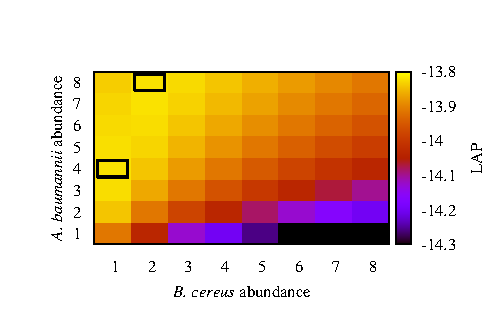
\includegraphics[width=4in]{ref_abun_1} \label{fig:ref_abun_1}}
\hfil
\subfigure[\emph{B. cereus} (4 copies, 5.2MB) and \emph{A. odontolyticus} (7 copies, 2.4MB)]{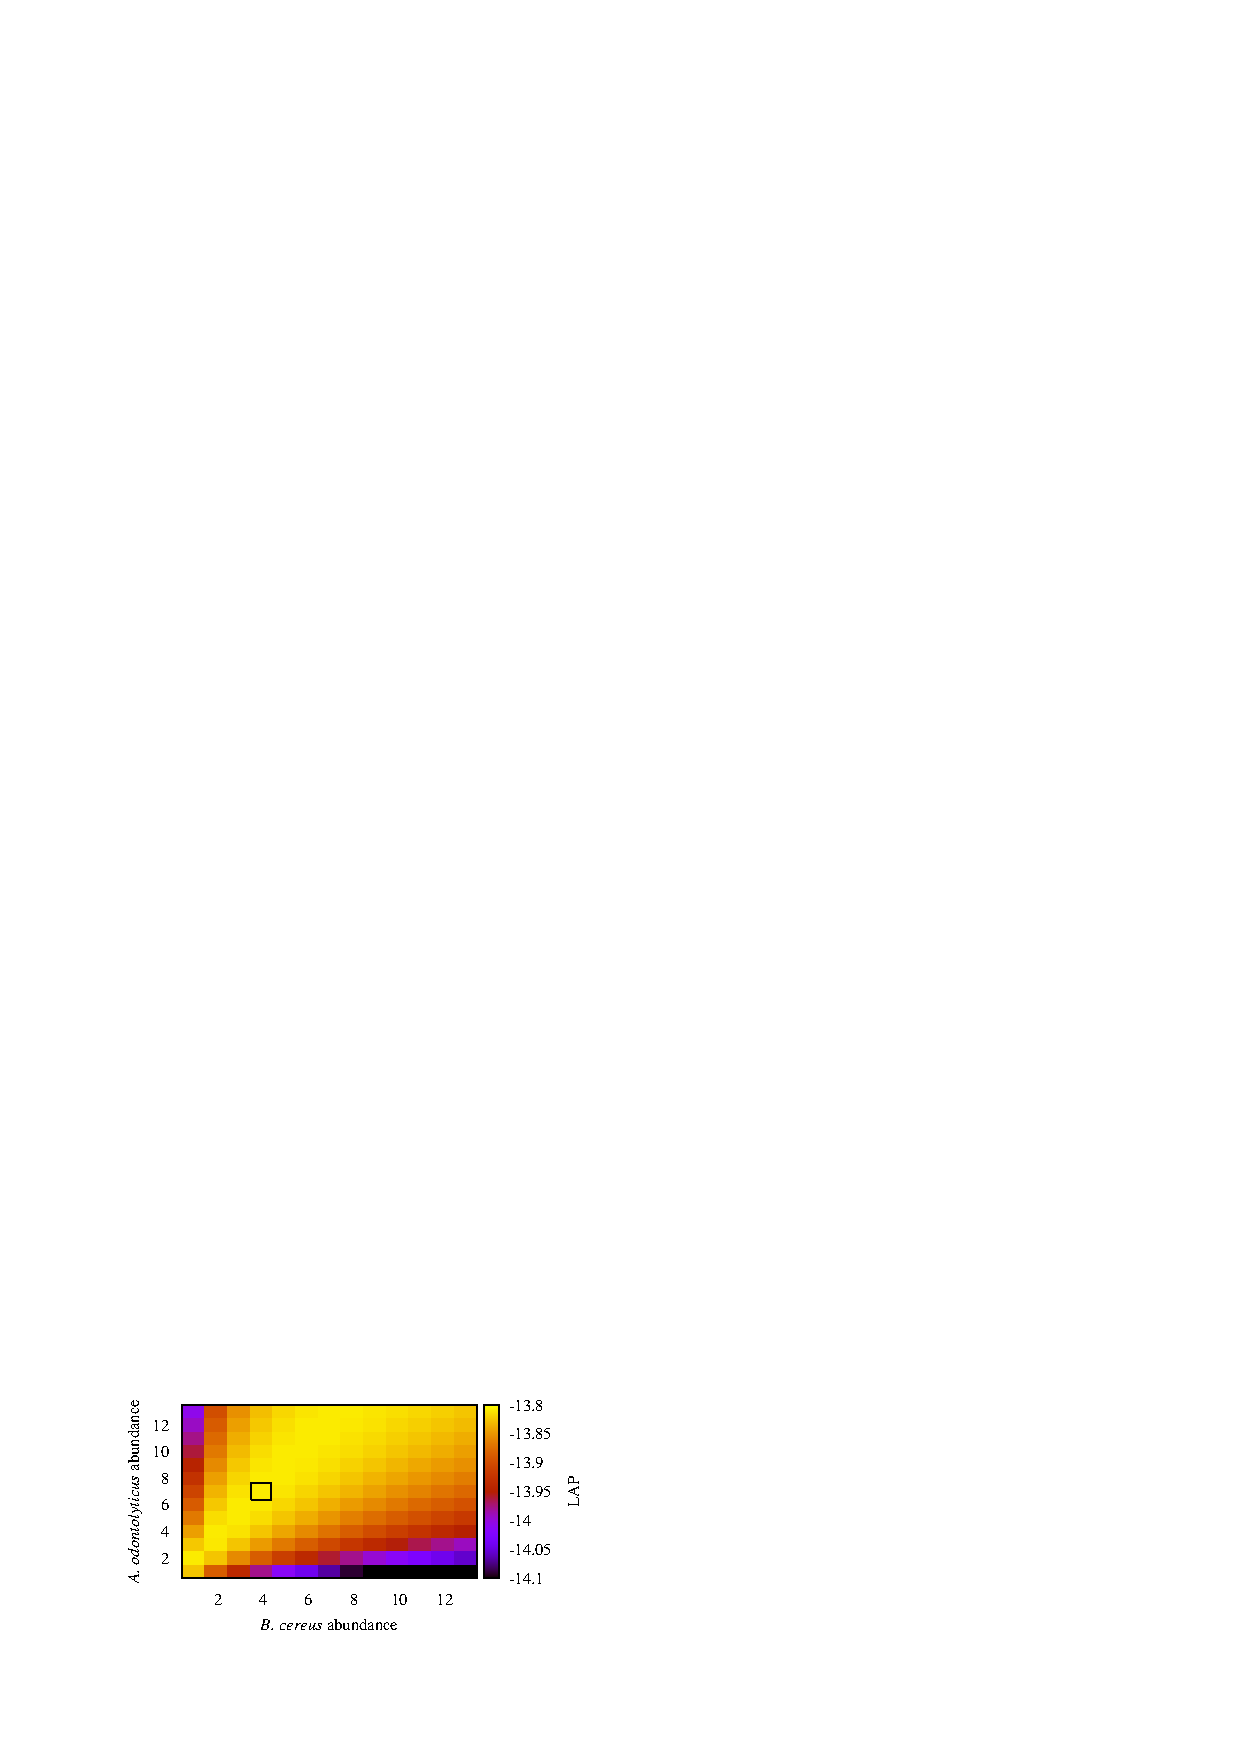
\includegraphics[width=4in]{ref_abun_2} \label{fig:ref_abun_2}}
\end{center}
\renewcommand{\baselinestretch}{1}
\small\normalsize
\begin{quote}
\caption[LAP scores for simulated metagenomic communities.] {LAP scores for simulated metagenomic communities. Each cell (x,y) represents the LAP score for a mixture of \emph{x} copies of the x-label bacteria and \emph{y} copies of the y-label bacteria.  In both groups, the true abundance ratios maximize the LAP score (indicated by a black rectangle in respective plots). \label{fig:ref_abun}}
\end{quote}
\end{figure}
\renewcommand{\baselinestretch}{2}
\small\normalsize
\newpage

\subsection{Extending LAP to metagenomic assemblies}

An important simplifying assumption of our framework is that the sequencing process is uniform in coverage.
In metagenomics, however, the relative abundances of organisms are rarely uniform~\cite{carrigg2007dna,krsek1999comparison,morgan2010metagenomic,temperton2009bias}, reflecting the difference in abundance between the different organisms within a community.
Here we show that taking this abundance information into account allows us to extend the LAP framework to metagenomic data.
%This feature makes using the LAP score incorrect out of the box.
%Later steps in the pipelines often deal with abundance estimation and phylogenetic classification.
We now assume that while the abundances of each organism may vary dramatically, the sequencing process still has uniform coverage across the \emph{entire} community.
%It is important to note while the abundances of each organism may vary dramatically, the sequencing process still produces a uniform coverage of the complete environment.
For example, consider a simple community containing two organisms (A and B), one which is twice as abundant as the other.
This community, thus, comprises twice as much of A's DNA than that of B.
Assume, for simplicity, that the community contains exactly three chromosomes (two of A and one of B).
A random sequencing process would sample each of these equally, and an ideal metagenomic assembler would produce two contigs, one covered twice as deep as the other.
%the case where we have three bacteria in an environment (1 copy of strain \emph{A}, 2 copies of strain \emph{B}).
%Now, lets assume we performed enough sequencing to produce a 1x coverage of each individual bacterium.
%An assembler would only output both bacteria strains, despite the difference in coverage.



In essence, we view the collection of individual genomes and their relative abundances as a single \emph{metagenome} where each genome is duplicated based on their abundance (\figurename~\ref{fig:metagenome}).
%Thus, we now assume we have uniform coverage across the entire metagenome.
This setting is similar to that of repeats in single genome assembly, where a repetitive element can now include an entire genome.
Like in the case of single genomes, the assembler that correctly estimates these repeat counts maximizes the LAP score.
In other words, in order to accurately evaluate the metagenomic assemblies using our LAP framework, the abundance (or copy number) of each contig is needed.
%The assembler that figures out the correct copy number of repeats (in this case, contigs) will have the highest LAP score.
As most metagenomic assemblers do not report this information,
here we use the average coverage of the contig (provided by the MetAMOS pipeline) to represent the copy number.

%In order to accurately calculate the LAP of a metagenomic assembly, in addition to the actual assemblies, we need the abundances.
In the error-free model, we compute the probability of a read, $p_r$, given the assembled sequence and abundance as:
%
\begin{equation}
  \label{meta_read_probability}
  p_r = \frac{\sum_{c \in \text{Contigs}}\text{abun}(c)*n_{rc}}{2\hat{L}}
\end{equation}
%
\begin{equation}
  \label{meta_read_length}
  \hat{L} = \sum_{c \in \text{Contigs}}\text{abun}(c)*L_{c}
\end{equation}
%
where $\text{abun}(c)$ is the abundance of contig c, $n_{rc}$ is the number of times read $r$ occurs in contig $c$, and $\hat{L}$ is the adjusted total assembly length.  In the case where the abundance of each contig is 1, calculating $p_r$ is identical to the original LAP (single genome) formulation.  A similar modification can be done to handle sequencing errors outlined in \cite{LAP}.

Our prior work has shown we can approximate the probabilities using fast and memory efficient search alignment programs (e.g., Bowtie2~\cite{langmead2012fast}) when it is impractical to calculate the exact probabilities for large read sets.
We can apply the metagenomics modification above to the alignment tool-based method:
%
\begin{equation}
\label{}
p_{r} = \frac{\sum_{j \in S_r} \text{abun}(j_{\text{contig}})*p_{r,j_{\text{subs}}}}{2\hat{L}}
\end{equation}
where $S_r$ is the set of alignments in the SAM file for the read $r$ and the probability of alignment, $p_{r,j_{\text{subs}}}$, is approximated by $\epsilon^{subs}(1 - \epsilon)^{l - subs}$ where $\epsilon$ is the probability of an error (a mismatch, an insertion, or a deletion).



%allow the assembler to tell us what copy number it expects for each contig - that is the average coverage for the contig (provided in our analysis by the MetAMOS pipeline).
%Our LAP framework uses the average per basepair coverage of assembled contigs provided by MetAMOS.

An important factor in any likelihood-based assembly evaluation framework is the handling of reads that do not align well to the given assembly.
In practice, unalignable reads are often the result of sequencing errors and contaminants.
If these reads are given a probability close to 0, then the best assembler would be the one that incorporates the most reads.
In our original LAP framework, a read that does not align well does not decrease the overall assembly probability more than the probability of an assembly that contains the appended read as an independent contig.
This does not change when we handle metagenomic data, since the average coverage of the ``new'' contig is one.

%However, commonly used metagenomic abundance tools are often targeted at taxonomic classification~\cite{segata2012metagenomic,brady2009phymm,liu2010metaphyler,huson2007megan}.
%One strategy to estimate contig abundances is to first perform taxonomic classification on the reads and then align the contigs with the taxonomic database, transitively applying the taxonomic abundances to the contigs.
%In lieu of taxonomic abundances, our LAP framework uses the average per basepair coverage of assembled contigs provided by MetAMOS.
%We use modified version of Sailfish\cite{sailfish}, a tool to quickly calculate transcript abundances using RNA-seq data, to estimate contig abundances.
%One of the underlying assumptions of Sailfish is that the coverage


% \begin{landscape}
% \renewcommand{\baselinestretch}{1}
% \small\normalsize
%
% \renewcommand{\baselinestretch}{2}
% \small\normalsize
% \end{landscape}



\subsection{Integration into MetAMOS}

In addition to being a standalone framework, the software implementing our metagenomic LAP approach comes packaged with the MetAMOS pipeline~\cite{koren2014automated}.
This allows users the option to run MetAMOS with different assemblers and have our framework automatically select the assembly with the highest LAP score without any prior knowledge from the user.
The first step of the MetAMOS pipeline is to \verb!Preprocess! the reads, optionally filtering out low quality reads.
Those reads are used by the next step \verb!Assemble!.
Users specify the desired assembler using the \verb!-a! parameter of \verb!runPipeline!.
We modified MetAMOS so users can now specify multiple assemblers (comma-separated) after the \verb!-a! parameter, and \verb!runPipeline! will run all assemblers and select the assembly yielding the highest LAP score to be used in downstream analyses.
%The software implementing our approach is made available, open-source and free of charge, at: \url{http://assembly-eval.sourceforge.net/} and with the MetAMOS package: \url{https://github.com/treangen/MetAMOS}.


\section{Results}
\subsection{Likelihood score maximized using correct abundances}
A key property of our framework is that the correct copy numbers (abundances) and assemblies maximizes our LAP score.
To illustrate this property, we simulated two metagenomic communities and calculated the LAP of the reference genomes with a combination of abundances.
The first simulated community consisted of \emph{Bacillus cereus} and \emph{Acinetobacter baumannii} at a ratio of 1:4.
We generated 200bp reads at 20x coverage of the metagenome (20x of \emph{B. cereus} and 80x of \emph{A baumannii}).
We calculated the LAP scores of the error-free reference genomes for all combinations of abundances (ranging from 1 copy to 8 copies) for each bacteria.
%We calculated the LAP score on error-free reference assemblies with all combinations of abundances from 1 copy to 8 copies for each bacteria.
The second simulated community consisted of \emph{Bacillus cereus} and \emph{Actinomyces odontolyticus} at a ratio of 4:7.
We generated 200bp reads at 20x coverage of the metagenome (80x of \emph{B. cereus} and 140x of \emph{A odontolyticus}).
We calculated the LAP scores of the error-free reference genomes for all combinations of abundances (ranging from 1 copy to 13 copies) for each bacteria.


%\begin{figure}[!t]
%\centering
%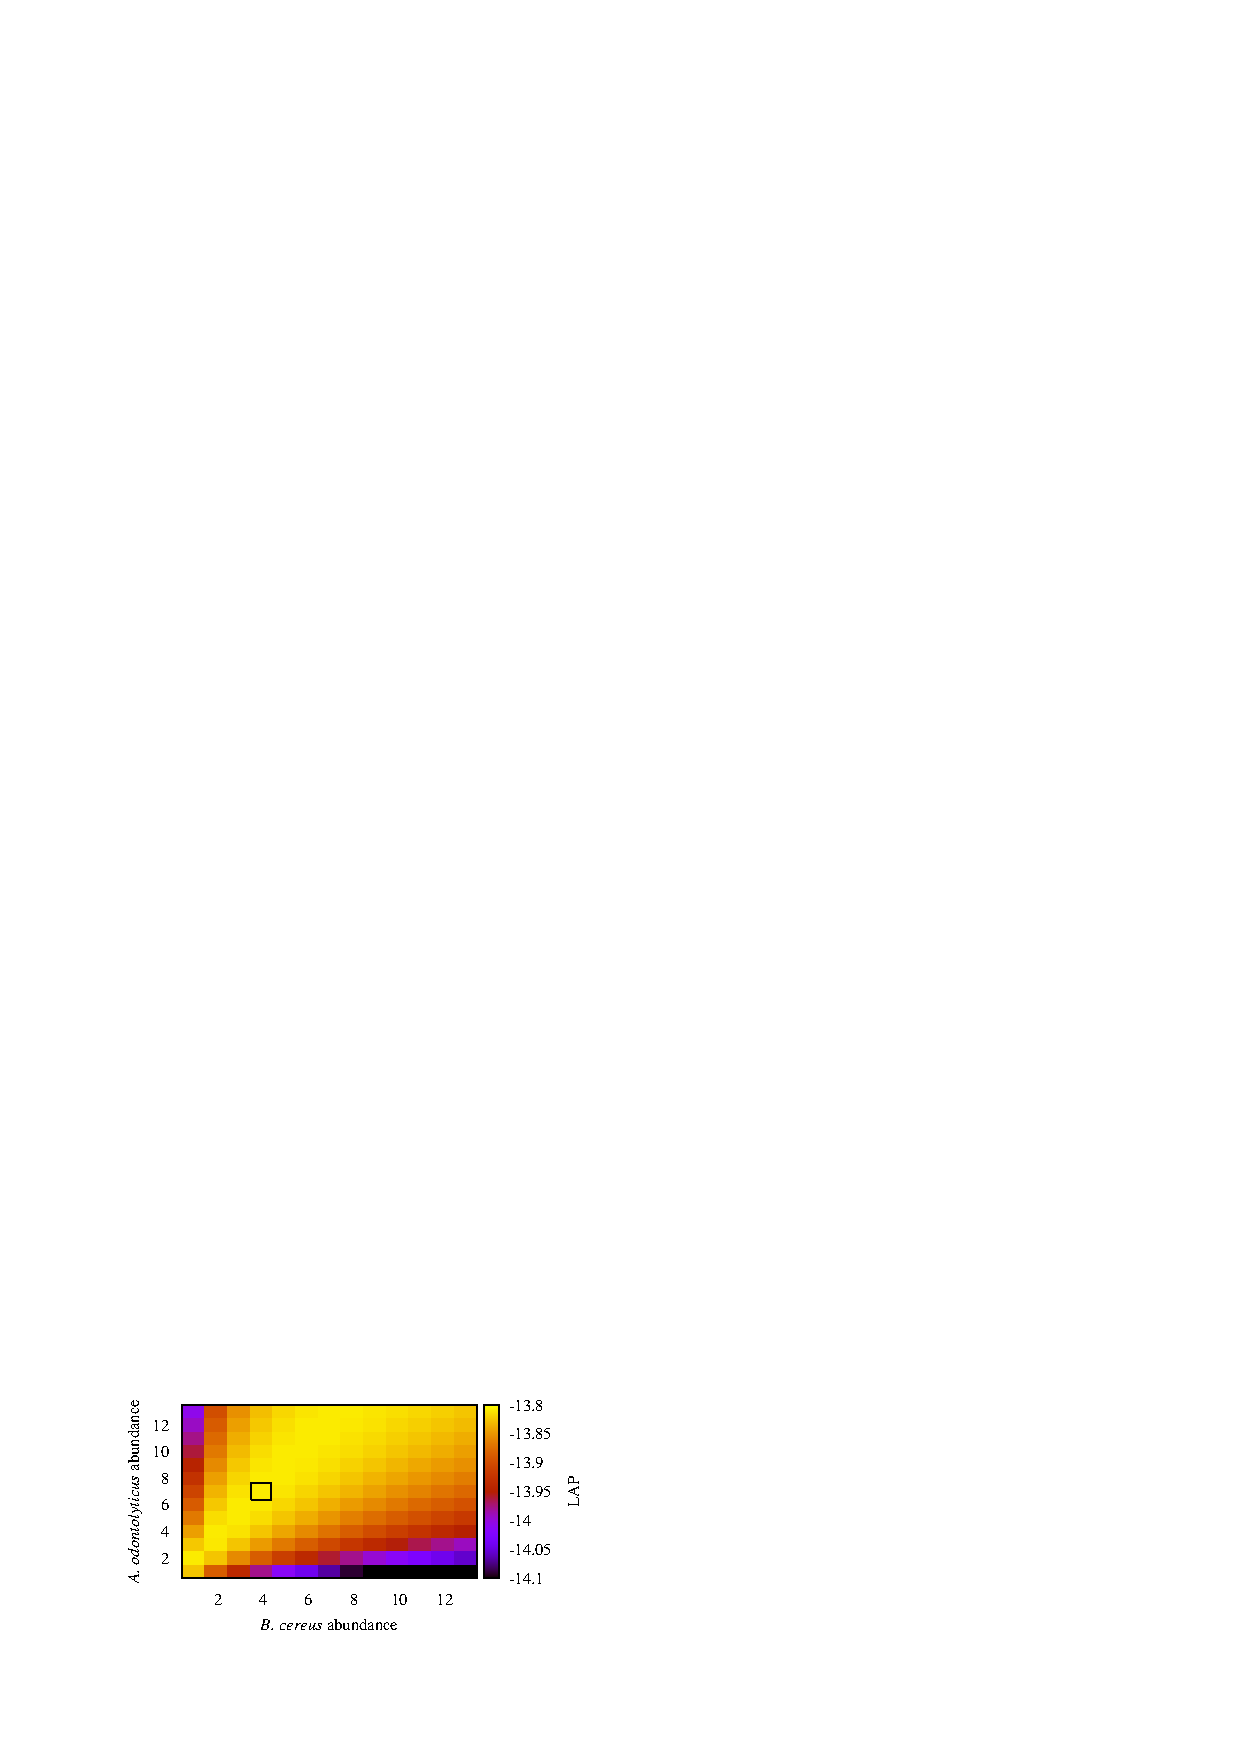
\includegraphics[width=3in]{ref_abun_2}
% where an .eps filename suffix will be assumed under latex,
% and a .pdf suffix will be assumed for pdflatex; or what has been declared
% via \DeclareGraphicsExtensions.
%\caption{LAP scores for simulated B. cereus (4x, 5.2MB) and A. odontolyticus (7x, 2.4MB)}
%\label{fig:ref_abun_2}
%\end{figure}

We expect the highest LAP scores for the assemblies that contain the correct abundance ratios (1:4 or 2:8 in the first community, and 4:7 in the second community).
%1:4 , 2:8 boxes to be highest in figure A, and 4:7, 8:14, etc. in panel 2.  Y
As seen in Figs. \ref{fig:ref_abun_1} and \ref{fig:ref_abun_2}, our LAP score is able to accurately reflect the varying organism abundance ratios present in the sample.
The LAP score increases as the estimates approach the true abundance ratios, with the true ratio yielding the highest LAP scores in both communities.

\begin{figure}[htb!]
\begin{center}
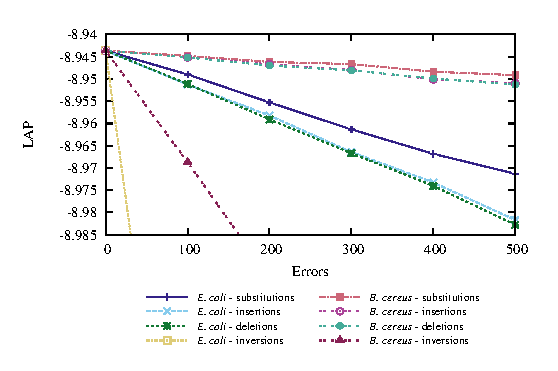
\includegraphics[width=.8\textwidth]{errors}
\end{center}
\renewcommand{\baselinestretch}{1}
\small\normalsize
\begin{quote}
\caption[Synthetic errors in simulated \emph{E. coli} and \emph{B. cereus} (1 copy, 5.2Mbp) community]{Synthetic errors in simulated \emph{E. coli} (5 copies, 4.9Mbp) \emph{B. cereus} (1 copy, 5.2Mbp) community.}
\label{fig:errors}
\end{quote}
\end{figure}
\renewcommand{\baselinestretch}{2}
\small\normalsize

\subsection{Impact of errors on synthetic metagenomes}

One of the often overlooked aspects of metagenomic assembly evaluation is the weighing of errors that occur in contigs with different abundances.
%In single genome assembly, errors are often not weighted since the genome has uniform coverage.
%When detecting errors with the aid of a reference, all substitution errors occurring within a genome are weighted the same (ignoring additional information, such as whether it occurs in a genic or regulatory element).
%When organism abundances are uniform, the weight of an assembly error is also uniform.
In metagenomic samples the relative organism abundances can vary by orders of magnitudes.
A typical reference-based evaluation would equally weight the errors irrespective of the abundance of the erroneous contigs.
The proposed metagenomic LAP score, however, automatically handles this situation and appropriately weighs errors according to genome abundance.
%Thus, errors in highly abundant organisms will have more of an impact on the LAP score than errors in organism of lower abundance.
To illustrate this, we simulated a small metagenomic community consisting of \emph{Escherichia coli} and \emph{Bacillus cereus} at a 5:1 ratio.
We introduced an increasing number of common assembly errors (single-base substitutions, insertions, deletions, and inversions) into the two organisms assemblies and observed the resulting LAP score.

As shown in \figurename~\ref{fig:errors}, the higher the number of synthetic errors, the lower the LAP score.
Insertions/deletions were more deleterious to the LAP score than substitutions, since in addition to causing a mismatch, an insertion/deletion changes the overall genome size.
Although inversions did not change the overall genome size (and would therefore not be detected by simplistic measures such as N50), these errors had the greatest impact on the LAP score because they prevented the alignment of reads across the boundaries of the inversions.
%With substitutions and indels, reads were still able to align across the error and only incurred the additional mismatch penalty.
%Conversely, read alignment tools will fail to detect read alignments that span the borders of the inversions.

%Whereas substitutions, insertions, and deletions still allowed reads to align albeit with a lower probability, reads that inversions are essentially treated as complete

As expected, errors introduced into the more abundant organism, \emph{E. coli}, had a greater affect on the LAP score than those inserted into \emph{B. cereus}.
Our LAP score was able to accurately weigh the errors by the abundance of each organism.


\subsection{Likelihood scores correlate with reference-based metrics}
%c|c|c|c|c|c


With real metagenomic samples, it is difficult to make evaluations given the lack of high quality references.
Using purely simulated data has the issue of not accurately capturing the error and bias introduced by sequencing technology.
Thus, to evaluate our LAP score, we use two `mock' communities (Even and Staggered) provided by the Human Microbiome Project (HMP) consortium\cite{mitreva2012structure,methe2012framework}.
These communities were created using specific DNA sequences from organisms with known reference genomes (consisting of over 20 bacterial genomes and a few eukaryotes) and abundances.
The mock Even community consisted of 100,000 16S copies per organism per aliquot, while the mock Staggered community consisted of 1,000 to 1,000,000 16S copies per organism per aliquot.
Data used from the HMP mock communities are available at \url{http://www.ncbi.nlm.nih.gov/bioproject/48475}.
We calculated the LAP score on assemblies produced by MetAMOS~\cite{treangen2013metamos} using several assemblers: SOAPdenovo~\cite{SOAPdenovo}, Metavelvet~\cite{namiki2012metavelvet}, Velvet~\cite{Velvet}, and Meta-IDBA~\cite{peng2011meta}.
The additional \emph{de novo} and reference-based metrics for the assemblies were taken from MetAMOS~\cite{treangen2013metamos}.  These metrics include:
   \begin{itemize}
   \item number contigs (\# ctgs) -- total number of contigs/scaffolds in the assembly
   \item good contigs (Good Ctgs) -- fraction of contigs that mapped without errors to reference genomes
   \item total aligned (Total aln) -- total amount of sequence (in Mbp) that can be aligned to the reference genomes
   \item slight mis-assemblies (Slt) -- alignments that cover 80\% or more of the aligned contig in a single match (Slt)
   \item heavy misassemblies (Hvy) -- alignments that cover less than 80\% of the aligned contig in a single match or have two or more matches to a single reference
   \item chimeras (Ch) -- contigs with matches to two distinct reference genomes
   \item size at 10 megabases (Size @ 10 Mbp) - the size of the largest contig $c$ such that the sum of all contigs larger than $c$ is more than 10 Mbp (similar to the commonly used N50 size)
   \item max contig size (Max ctg size) -- size of the largest contig in the assembly
   \item errors per megabase (Err per Mbp) -- average number of errors per Mbp in the assembly
   \end{itemize}

Generally, the \emph{de novo} LAP scores agree with the referenced-based metrics (Table \ref{tab:hmp}).
In the mock Even dataset, SOAPdenovo has the greatest LAP score, the highest fraction of contigs that can align to a reference genome without error, total amount of sequence that can be aligned to a reference genome, while also having the lowest amount of misassemblies (including chimeric) and errors per Mbp.
It is important to note that if user selected an assembly based on the best contiguity at 10Mbp, they would select the MetaVelvet assembly, which contains double the error rate per Mbp as the SOAPdenovo assembly while aligning 2Mbp less to the references.

\begin{figure}[tb!]
\begin{center}
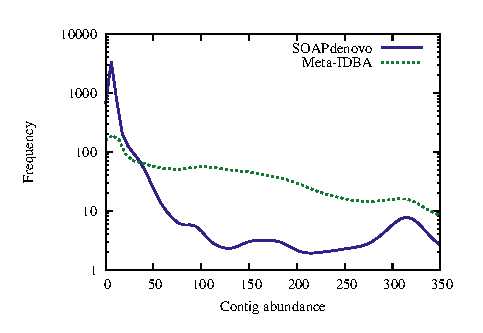
\includegraphics[width=.8\textwidth]{coverage}
\end{center}
\renewcommand{\baselinestretch}{1}
\small\normalsize
\begin{quote}
\caption[Frequency of contig abundances for assemblies of the HMP mock Staggered dataset]{Frequency of contig abundances for assemblies of the HMP mock Staggered dataset.}
\label{fig:coverage}
\end{quote}
\end{figure}
\renewcommand{\baselinestretch}{2}
\small\normalsize


\begin{landscape}
\renewcommand{\baselinestretch}{1}
\small\normalsize

\begin{table}[tbp]
\renewcommand{\arraystretch}{1.2}
\centering
\scriptsize
\begin{tabular}{{l}{l}{c}{c}{c}{c}{c}{c}{c}{c}{c}{c}{c}}
\hline
\bfseries Dataset & \bfseries Assembler & \bfseries LAP & \bfseries \#ctgs &  \bfseries Good ctgs & \bfseries Total aln & \bfseries Slt & \bfseries Hvy & \bfseries Ch & \bfseries Size @ 10 Mbp &\bfseries Max ctg size & \bfseries Err per Mbp & \bfseries Aligned reads \\
\hline\hline

mockE & SOAPdenovo & \textbf{-27.031} & 63107 & \textbf{99.3\%} & \textbf{51} & \textbf{166} & 131          & \textbf{1} & 28,208          & 249,819          & \textbf{5.8}  & \textbf{85.75\%} \\
mockE & Velvet     & -28.537          & 12,830 & 96.2\%          & 41          & 256          & \textbf{100} & 2          & 42,269          & 179,673          & 8.7  & 83.30\%        \\
mockE & MetaVelvet & -27.102          & 22,772 & 96.8\%          & 49          & 462          & 156          & 4          & \textbf{62,138} & \textbf{367,458} & 12.7    & 85.65\%      \\
mockE & Meta-IDBA  & -31.166          & 22,032 & 95.4\%          & 47          & 362          & 151          & 3          & 26,141          & 249,069          & 11  & 81.81\%\\
\\
mockS & SOAPdenovo & -60.161          & 44,928 & \textbf{98.8\%} & \textbf{28} & 135          & 98           & \textbf{0} & 5,672           & 186,064          & \textbf{8.3} & 69.78\%  \\
mockS & Velvet     & -60.711          & 21,050 & 95.8\%          & \textbf{28} & 485          & 115          & 1          & 6,060           & 119,120          & 21.5          & 67.26\% \\
mockS & MetaVelvet & -60.442          & 20,551 & 95.3\%          & \textbf{28} & 517          & 143          & 3          & 6,685           & \textbf{217,330} & 20.1         & 67.72\% \\
mockS & Meta-IDBA  & \textbf{-58.851} & 4,559  & 92.5\%          & 18          & \textbf{101} & \textbf{83}  & \textbf{0} & \textbf{13,150} & 119,604          & 10.2  & \textbf{70.67\%}\\
\\
Tongue  & SOAPdenovo & \textbf{-13.844} & 35,230 & \textbf{89.10\%} & \textbf{11} & 1,138 & 2,618 & \textbf{0} & 11,359 & \textbf{238,051} & \textbf{341.5} & \textbf{88.14\%}\\
Tongue  & Meta-IDBA & -21.368 & 25,698 & 88.70\% & 7 & \textbf{710} & \textbf{2,087} & \textbf{0} & 4,215 & 59,188 & 399.6 & 58.89\% \\

\hline
\end{tabular}
\caption[Comparison of assembly statistics for HMP mock Even and mock Staggered datasets]{Comparison of assembly statistics for HMP mock Even and mock Staggered datasets.Numbers in bold represent the best value for the specific dataset.}
\label{tab:hmp}
\end{table}

\renewcommand{\baselinestretch}{2}
\small\normalsize
\end{landscape}


Since the abundances of each organism in the mock Even dataset are fairly similar, the mock Staggered abundance distribution creates a more realistic scenario encountered in metagenomic environments.
Here, the Meta-IDBA assembly has the greatest LAP score, but aligns roughly a third less sequences to the reference genomes than SOAPdenovo.
The Meta-IDBA assembly contains approximately a tenth of the amount of contigs (4,559 vs. 44,928) as SOAPdenovo.
The SOAPdenovo assembly contains a greater number of contigs at a very low abundance (\figurename~\ref{fig:coverage}).
On large contigs Meta-IDBA performs better than SOAPdenovo and has a lower error rate (see \figurename~4 in \cite{treangen2013metamos}).
However, Meta-IDBA assembles a smaller fraction of the low-abundance genomes than SOAPdenovo, leading fewer sequences to align.
The LAP score penalizes misassemblies within abundant contigs in the SOAPdenovo results.


%Given how the mock Staggered community was constructed (each ratio of 16S copies per aliquot occurred roughly the same number of times), the frequency of contig abundances should be approximately uniform for the community.
%The SOAPdenovo assembly was able to align more reads, but the reads were localized in these low coverage regions.
%The distribution of contig abundances in the Meta-IDBA assembly was closer to the expected distribution than the SOAPdenovo assembly.

%The Meta-IDBA assembly a far more uniform frequency of contig abundances compared to the SOAPdenovo assembly.

Next, we applied our framework on real data where we did not know the actual genomes comprising the sample (HMP tongue dorsum female sample, SRS077736) (Table \ref{tab:hmp}).
Although we do not know for certain which organisms are present in the sample, the HMP identified a reference genome set with high similarity to the sequences within the sample (HMP Shotgun Community profiling SRS077736).
The reference-based error metrics only consider chimeric errors due to the possibility of structural difference between an organism and its version in the reference database.
We calculated the LAP of the assemblies using a single library consisting of 42,013,917 reads.
The SOAPdenovo assembly had a far greater LAP score than the Meta-IDBA assembly.
The higher score is due to the SOAPdenovo assembly recruiting more reads (88.14\% to 58.89\%) in relation to its genome size (46Mbp to 37Mbp) than the Meta-IDBA assembly.
Furthermore, the MetAMOS metrics show that the SOAPdenovo assembly contained approximately 60 less errors per Mbp than the Meta-IDBA assembly.

%These datasets have the advantage over simulated data because it captures the error and bias introduced from the sequence technology.


\renewcommand{\baselinestretch}{1}
\small\normalsize

\begin{table}[tb!]
\label{tab:metamos_lap}
\centering
\begin{tabular}{{l}{c}{c}{c}{c}}
\hline
\bfseries Assembler & \bfseries Contigs & \bfseries LAP & \bfseries N50 (Kbp) & \bfseries  Errors \\
\hline \hline
newbler  & \bf{1} & \bf{-13.064} & \bf{156} & 1 \\
SOAPdenovo & 23 & -14.238 & 9 & \bf{3} \\
Velvet & 3 & -13.157 & 92 & \bf{0} \\
MetaVelvet & 3 & -13.157 & 92 & \bf{0} \\
\hline
\end{tabular}
\caption[Self-tuning MetAMOS using \emph{C. ruddii} test dataset]{Self-tuning MetAMOS using \emph{C. ruddii} test dataset.}
\end{table}

\renewcommand{\baselinestretch}{2}
\small\normalsize

\subsection{Tuning assembly parameters for MetAMOS}
Assemblathon1~\cite{earl2011assemblathon} has shown that assembly experts can often get drastically different assemblies using the same assemblers, highlighting the difficulty of choosing the \emph{right} parameters for a given assembler.
Our metagenomic LAP framework comes packaged with the MetAMOS pipeline, allowing users the option to run MetAMOS with different assemblers and automatically select the assembly with the highest LAP score.
This step occurs without any prior knowledge from the user.

We showcase the ease of use of the automated assembler selection within MetAMOS using the \emph{Carsonella ruddii} (156Kbp) dataset packaged with MetAMOS (Table ~\ref{tab:metamos_lap}).
Errors were found using DNADIFF~\cite{phillippy2008genome} and MUMmer~\cite{delcher2003using}.
The newbler assembly produced one contig containing the complete \emph{C. ruddii} genome.
The SOAPdenovo assembly produced a severely fragmented assembly with the most number of errors.
The MetaVelvet and Velvet produced identical assemblies, containing 3 contigs of sizes 92Kbp, 65Kbp, and 1.7Kbp, but contained an additional 158bp compared to the \emph{C. ruddii} genome.
Upon closer inspection, there were overlaps between the contigs ranging from 38bp to 73bp.
This is not surprising given MetaVelvet's and Velvet's de bruijn graph-based approach could not resolve repetitive regions between the contigs.
Newbler, on the other hand, contained only a single insertion error.
The LAP score of the Newbler assembly was greater due to more reads being able to align across the regions that were broken apart in the MetaVelvet and Velvet assemblies.
Additionally, the Newbler assembly did not contain the duplicated sequence found in the other assemblies.
MetAMOS was able to select the most likely assembly without requiring any additional input from the user.

\section{Discussion}

In this chapter, we have proposed an extension to our LAP framework to perform \emph{de novo} comparisons of metagenomic assemblies.
Unlike traditional \emph{de novo} metrics used for measuring assembly quality, our extended LAP score correlates well with reference-based measures of metagenomic assembly quality.
However, in this study, we have realized that there is a lack of reference-based metrics when evaluating metagenomic assemblies.
Misjoins betweens organisms may be more deleterious than misjoins within a single genome.
Furthermore, current reference-based metrics do not take into account the relative abundances of the organisms when evaluating metagenomic assemblies.
The metrics provided by MetAMOS do not factor in the contig abundances when examining assembly errors.
This made it difficult to compare our LAP score to their reference-based metrics because, intuitively, an error in a highly abundant organism should be \emph{worse} than an error in a rare, low coverage organism.
Our LAP score implicitly weighs the errors in abundant contigs more than those in lesser abundant contigs.
In our results, we have proposed one such reference-based metric that scales the errors by the relative abundance of the contig it occurs within.

It is important to note that we have only focused on the complete reconstruction of the metagenome from the set of reads.
Assembly algorithms are designed with specific biological applications in mind, such as, the conservative reconstruction of the genic regions.
Studies focusing on the genic regions may tolerate large-scale rearrangements as long as the genic regions were correctly assembled.
Conversely, other studies may want to focus on the reconstruction and detection of rare pathogenic bacteria in an environment.
These application specific assembly algorithms all attempt to optimize their formulation of the assembly problem.

Our metagenomic LAP extension relies heavily on the idea that the sequencing process of the metagenome is roughly uniform, and that the reads are independently sampled from the genome.
Biases exist in all steps of the sequencing process, from the extraction of DNA from organisms with different cell membranes/walls~\cite{carrigg2007dna,krsek1999comparison} to the sequencing protocol used~\cite{morgan2010metagenomic,temperton2009bias}.
In the future, we would like to implement a more specific model that better captures the sequencing process.

%De novo metric, more misleading in assemblies -> chimera

%We would like to stress that \emph{de novo} measures of assembly quality, such as ours, are critically needed by researchers attempting to assemble of yet unknown genomes.

Results from GAGE~\cite{salzberg2011gage} and Assemblathon~\cite{earl2011assemblathon,bradnam2013assemblathon} have shown that the specific characteristics of the data being assembled has a great impact on the performance of the assembler.
This problem is magnified in metagenomic assembly.
By integrating our LAP framework in MetAMOS, we have allowed researchers to accurately and effortlessly run and evaluate assemblies without any prior knowledge on evaluating assembly quality.

In our framework, we use the average coverage of the contig (provided by MetAMOS) to estimate abundance.
There are issues with this measure as it is possible that mis-assembled repeats within a contig will affect our estimate of depth of coverage and could impact our underlying statistics.
A better approach is to use something more robust than the mean coverage, such as the median coverage, to avoid being influenced by such regions.
While the user can supply the median coverage to our standalone framework, future work includes building this feature into MetAMOS.
Another approach involves breaking contigs at regions of differing coverage (using tools such as AMOSvalidate\cite{phillippy2008genome}), so there will be less deviation in the average coverage within the contig.

It should be noted that in some cases it may not be tractable to run the complete collection of assemblers with MetAMOS.
In such cases, we should first employ heuristics (such as \cite{chikhi2013informed}) to aid in selecting potential assemblers (and parameters) to run.
For the assembler selection process, we can use the LAP framework's sampling procedure in combination with calculating read probabilities in parallel to reduce runtime.

Our goal was to provide a global measure of how good a metagenomic assembly may be, not to detect assembly errors.
Other likelihood-based frameworks, such as ALE, use frequencies of certain sequences to aid in detection of possible chimeric contigs.
We are able to apply similar modifications to our LAP framework to find regions of possible misassembly.
Finally, we plan to extend our framework to give a more detailed breakdown of the LAP scores of segments assembled using the same subset of reads across different assemblies.
The goal would be to take high-scoring assembled segments from individual assemblies to recreate an assembly with overall greater likelihood.
This approach will be of great benefit to the field of metagenomic assembly since assemblers are often designed with different constraints and goals in mind, e.g., low memory footprint, assembling high/low coverage organisms, or tolerating population polymorphisms.
For example, on the mock Staggered dataset, Meta-IDBA best assembled the most abundant genomes while SOAPdenovo had a better representation of the low abundance organisms.
Providing a systematic way of combining assembler approaches using our LAP score will produce better assemblies for downstream analyses.


% An example of a floating figure using the graphicx package.
% Note that \label must occur AFTER (or within) \caption.
% For figures, \caption should occur after the \includegraphics.
% Note that IEEEtran v1.7 and later has special internal code that
% is designed to preserve the operation of \label within \caption
% even when the captionsoff option is in effect. However, because
% of issues like this, it may be the safest practice to put all your
% \label just after \caption rather than within \caption{}.
%
% Reminder: the "draftcls" or "draftclsnofoot", not "draft", class
% option should be used if it is desired that the figures are to be
% displayed while in draft mode.
%
%\begin{figure}[!t]
%\centering
%\includegraphics[width=2.5in]{myfigure}
% where an .eps filename suffix will be assumed under latex,
% and a .pdf suffix will be assumed for pdflatex; or what has been declared
% via \DeclareGraphicsExtensions.
%\caption{Simulation Results}
%\label{fig_sim}
%\end{figure}

% Note that IEEE typically puts floats only at the top, even when this
% results in a large percentage of a column being occupied by floats.


% An example of a double column floating figure using two subfigures.
% (The subfig.sty package must be loaded for this to work.)
% The subfigure \label commands are set within each subfloat command, the
% \label for the overall figure must come after \caption.
% \hfil must be used as a separator to get equal spacing.
% The subfigure.sty package works much the same way, except \subfigure is
% used instead of \subfloat.
%
%\begin{figure*}[!t]
%\centerline{\subfloat[Case I]\includegraphics[width=2.5in]{subfigcase1}%
%\label{fig_first_case}}
%\hfil
%\subfloat[Case II]{\includegraphics[width=2.5in]{subfigcase2}%
%\label{fig_second_case}}}
%\caption{Simulation results}
%\label{fig_sim}
%\end{figure*}
%
% Note that often IEEE papers with subfigures do not employ subfigure
% captions (using the optional argument to \subfloat), but instead will
% reference/describe all of them (a), (b), etc., within the main caption.


% An example of a floating table. Note that, for IEEE style tables, the
% \caption command should come BEFORE the table. Table text will default to
% \footnotesize as IEEE normally uses this smaller font for tables.
% The \label must come after \caption as always.
%
%\begin{table}[!t]
%% increase table row spacing, adjust to taste
%\renewcommand{\arraystretch}{1.3}
% if using array.sty, it might be a good idea to tweak the value of
% \extrarowheight as needed to properly center the text within the cells
%\caption{An Example of a Table}
%\label{table_example}
%\centering
%% Some packages, such as MDW tools, offer better commands for making tables
%% than the plain LaTeX2e tabular which is used here.
%\begin{tabular}{|c||c|}
%\hline
%One & Two\\
%\hline
%Three & Four\\
%\hline
%\end{tabular}
%\end{table}


% Note that IEEE does not put floats in the very first column - or typically
% anywhere on the first page for that matter. Also, in-text middle ("here")
% positioning is not used. Most IEEE journals/conferences use top floats
% exclusively. Note that, LaTeX2e, unlike IEEE journals/conferences, places
% footnotes above bottom floats. This can be corrected via the \fnbelowfloat
% command of the stfloats package.



\section{Conclusion}
In this chapter we have described an extension to our \emph{de novo} assembly evaluation framework (LAP) for comparing metagenomic assemblies.
We showed that the true metagenome and correct relative abundances maximizes our extended LAP score.
Furthermore, we have integrated our framework into the metagenomic assembly pipeline MetAMOS, showing that any user is able to reproduce quality evaluations of metagenomic assemblies with relative ease.

\renewcommand{\thechapter}{4}
\chapter{Regression Testing of Genome Assemblers}
\section{Introduction}

The issues with testing ``non-testable programs'' were first raised by Davis
and Weyuker in a 1981 paper \cite{Davis:1981:PNP:800175.809889}. An important
characteristic of such programs is the absence of a {\it test oracle}, the
mechanism that determines whether a software under test (SUT) executed
correctly for a test case.  Without a test oracle, a test case has no way to
{\it pass} or {\it fail}. This calls into question the overall purpose and
value of software testing.

Although there has been work in the area of testing such non-testable programs
\cite{McMinn:2009:SFD:1569901.1570127,Murphy:2010:MTT:1970820,Murphy:2009:AST:1572272.1572295,Yoo:2010:MTS:1799526.1799581,Chan:2010:FFP:1815297.1815298,Chen:2002:SIM:566172.566202,Lazic:2005:AMS:1983314.1983364,Just:2010:AST:1808266.1808280,Just:2011:AUI:2036458.2036488},
in practice this problem continues to be a significant hurdle for test
automation in many scientific domains, where it is either very expensive or
impossible to determine the correct answer for a scientific problem
\cite{Hook:2009:TTS:1556904.1556936} (e.g., validating machine learning
classifiers \cite{Xie:2011:TVM:1942318.1942371}, analyses of feature models
\cite{Segura:2011:AMT:1937186.1937327}) or computation (e.g., processing large
XML files \cite{Kim-Park:2010:ATO:1868048.1868050}.  image segmentation
\cite{Frounchi:2011:AIS:2038078.2038454}, mesh simplification
\cite{chan2009pat}).  This is especially problematic for the
domain of bioinformatics, a largely software-intensive field. Bugs in
bioinformatics software have the potential to lead to incorrect scientific
conclusions.  As observed by Chen et al.  \cite{BMC}, ``{\it incorrectly
computed results may lead to wrong biological conclusion, and ...
misguide downstream experiments}.''

Consider the classic problem in bioinformatics -- {\it de novo genome sequence assembly}.  The
{\it genome sequence} of an organism is important for understanding its life
cycle and evolution.  Current sequencing technology is only able to produce
{\it reads} (sequenced fragments) that are drastically shorter than the genome.
Therefore, in order to carry out meaningful biological analyses, one must first
{\it assemble} the original genome using {\it assemblers}.  The result of the
assembly is one or more {\it contigs} (contiguous sequence fragments) that can
be ordered and oriented into {\it scaffolds} with {\it gaps} (unknown parts in
the sequence).  Current formulations of the genome assembly problem are
optimization problems on graphs, which are known to be NP-hard
\cite{medvedev2007computability}.  In practice, assemblers are only able to
return an approximate solution.

Because of the nature of the domain, it is very difficult to validate the
correctness ({\it quality} \cite{monya2012}) of an assembly -- the
correct/expected solution is not known.  In software testing terms, the {\it
test oracle} is unavailable.
Moreover, when researchers develop a new
assembler, they often run it on a new dataset, making comparisons difficult.
Monya \cite{monya2012} notes that the bioinformatics community needs to find
``{\it ways to assess and improve assemblers in general.}''

Hence, the community faces the following scenario: {\it iteratively improve
the assember}, ensuring at each step that the assembly did indeed improve, and
that no new bugs that might degrade the assembler's output were introduced.
This puts us in the realm of {\it regression testing}.  One way to determine
whether bugs have not degraded a software's output is by using what we call a
{\it diff}-based approach, i.e., running test cases on the old and new versions
of the code and identifying differences in the tests' outcome
\cite{Orso:2008:BBR:1401827.1401835}.  Thus, regression testing employed by
assemblers may compare the text output of an assembler on test datasets with
previously computed assemblies to determine if the code changes produced a
different assembly.  Comparing the raw text outputs of an assembler is not
robust enough to capture whether there were actual differences in the quality
of assembly. Multiple assemblies of the same set of \emph{reads} are acceptable as correct. Reordering the reads may produce different
assemblies that have the same overall quality, but contain trivial differences,
such as the assembly starting a different position in circular bacteria genome (Fig. \ref{fig:circular_genome}).
%Reads and assemblies are stored in the FASTA format, where each entry consists of a single line descriptor starting with \verb|>| symbol, followed by the biological sequence.


\begin{figure}[!htb]%figure2
\begin{center}
%\includegraphics[width=4in]{preprocessing_results.pdf}
\begin{verbatim}
>sample circular sequence
AGCATCTTTATTGGAGATGTGCCACAGCACATTG
\end{verbatim}
  %\end{minipage} GCTTTGGTGGGTTTACATTTAAAAGAACAAGCGGGT
  %\begin{minipage}{.2\linewidth}
\begin{center}
\line(1,0){200}
\end{center}
\begin{verbatim}
>sample circular sequence rotated 1 char
GAGCATCTTTATTGGAGATGTGCCACAGCACATT
\end{verbatim}
\end{center}
\renewcommand{\baselinestretch}{1}
\small\normalsize
\begin{quote}
\caption[FASTA file containing two entries that represent the same circular sequence.]{FASTA file containing two entries that represent the same circular sequence. Each entry consists of a single line descriptor starting with the $>$ symbol, followed by the biological sequence. Text comparison tools would detect that these two sequences are different.}
\label{fig:circular_genome}
\end{quote}
\end{figure}
\renewcommand{\baselinestretch}{2}
\small\normalsize

\iffalse
To illustrate the inadequacy of previous assembly regression testing, we use two assemblers, SOAPdenovo \cite{li2010novo} and Minimus of the AMOS package \cite{sommer2007minimus}.
We run SOAPdenovo and Minimus on the \emph{Rhodobacter sphaeroides} fragment library (1,408,188 reads of length 101 bp) using the original reads, along with a shuffled version of the original reads and perform the unix command \textbf{diff} on the output.
Since SOAPdenovo allows the use of multiple threads, we run the assembler using one and eight threads.
Both assemblers produce different assemblies depending on whether they use the original or shuffled reads (Table \ref{Tab:01}).
By doing a \textbf{diff} of the text outputs we are unable to determine if there is a non-trivial change in assembly quality.


%AMOS is a set of open-source whole genome assembly tools \cite{sommer2007minimus}.  Developers at different institutions are involved in the development of AMOS.  Whenever a developer makes a change to the code, it is tested on the developer’s local hardware, ensuring that the code changes do not produce different assemblies.


\renewcommand{\baselinestretch}{1}
\small\normalsize

% \renewcommand{\baselinestretch}{2}
% \small\normalsize

\begin{table}[h]
%\processtable{Using rhodobacter ALLPATHS-LG corrected fragment library.}
%{\tiny
\caption{For Minimus and SOAPdenovo, we check if assemblies produced from the original and shuffled reads are the same by doing a \textbf{diff} of the resulting assembly text files.  In addition, we also find that the assemblies produced using different number of threads differ in SOAPdenovo.  Assemblers used rhodobacter ALLPATHS-LG corrected fragment library. 1408188 reads.}
\label{Tab:01}
\begin{tabular}{r|cc}
& Minimus & SOAPdenovo \\ \hline
Original vs. shuffled reads & Not equal & Not equal \\
1 vs. 8 threads & NA & Not equal \\ \hline
\end{tabular}
%{\tiny {Table 1. Using rhodobacter ALLPATHS-LG corrected fragment library. 1408188 reads.  For Minimus and SOAPdenovo, we check if assemblies produced from the original and shuffled reads are the same by doing a diff of the resulting assembly text files.  In addition, we also find that the assemblies produced using different number of threads differ in SOAPdenovo.}}
%}
\end{table}
\fi
\renewcommand{\baselinestretch}{2}
\small\normalsize


In this chapter, we present a novel assembler-specific regression testing
framework that uses two assembly evaluation mechanisms: \emph{assembly likelihood}, calculated using LAP\cite{LAP}, and \emph{read-pair coverage}, calculated using REAPR\cite{hunt2013reapr}, to determine if code modifications result in non-trivial
changes in assembly quality. The log average probability, LAP, is
the log of the geometric mean of the probability that the observed reads are generated from the given assembly.
By modeling the sequencing process, we are able to accurately calculate this probability. REAPR is
tool for detecting misassemblies using the coverage of read-pairs.

We evaluate our framework using SOAPdenovo \cite{li2010novo} and Minimus \cite{sommer2007minimus}.
SOAPdenovo is a widely popular \emph{de novo} assembler designed for short reads that has been used in many high profile genome assemblies, including the giant panda \cite{li2009sequence}.
Minimus is one of the several assembly pipelines in the AMOS software package.
Minimus provides a good case study for software engineering in bioinformatics due to its open-source nature, modular design, and active developer community.

We study assembler evolution in two contexts. First,
we examine how assembly quality changes
throughout the version history of SOAPdenovo. Second,
we show that our framework can correctly evaluate decrease in assembly quality
using fault-seeded versions of Minimus.
Our results show that our framework accurately detects trivial
changes in assembly quality produced from permuted input reads and using
multi-core systems, which fail to be detected using traditional regression
testing methods.

Here we make the following contributions:

\begin{itemize}

\item
%{\bf Chris: say something about a fundamental contribution for bioinformatics.}
Provides a regression testing framework novel to the domain of \emph{de novo} genome assembly.
%, saving developer resources.

\item
%{\bf Chris: say something about a fundamental contribution for software
%testing. For example, we develop a mechanism that can be used in other software
%testing situations?}
Illustrates the benefits of developing a regression testing framework for untestable software leveraging existing third party tools.
%Shows that is still useful to leverage existing

\item
%{\bf Chris: say something about our experiments. For example, others can
%use the subjects, versions, etc.}
\emph{All} of the software from our regression testing framework, experimental sequence data, assemblers, and results are available online.

\end{itemize}

We believe that this research is both timely and relevant.  As sequencing
technology becomes cheaper, assemblers will operate on increasingly larger data
sets, \emph{requiring} large multi-core machines in order to assemble these
datasets in a reasonable time frame.  Developers need to design test cases
that match the complexity and size of practical datasets to adequately test
their assembler.  Depending on the underlying algorithms, concurrent programs
may produce different outputs.  Assemblers may produce slightly different
assemblies than their single-threaded version, making it difficult to compare
the raw text outputs.

% \noindent{\bf Structure of the paper:}
In the next section,
we describe how the problem of testing without an oracle is not limited to bioinformatics, and the different strategies typically used and their limitations.
In Section~\ref{methods}, we describe our regression testing approach, briefly outlining the theory behind assembly likelihood and read-pair coverage and why they are our main measure of assembly quality.
% we provide an overview of our approach via an example, showing how {\it diff} is not a correct means of assessing differences in assembly quality.
%In Section~\ref{methods}, we briefly describe the theory behind why the LAP is the main measure of assembly quality in our regression testing framework, along with the purpose of including amosValidate.
In Section~\ref{results}, we show how our framework is able to accurately evaluate the trivial changes in assembly quality using real sequencing data.  Then, we examine how assembly quality changes throughout the release history of SOAPdenovo.  We wrap up our results showing the fault detection power of our framework using manually seeded faults within Minimus.
In Section~\ref{discussion}, we discuss the significance and limitations of our framework, and the lack of adequate testing within the assembler community.
Finally, in Section~\ref{conclusion}, we conclude with a discussion of future research directions.

\section{Related work}
\label{related_works}
The difficulty in software testing without an oracle is not limited to genome assembly,
 but has been encountered in many other fields such as bioinformatics, weather prediction, and image and speech processing. In bioinformatics, for example, a common task is to
find all potential mappings of a sequence to another reference sequence which contains at most a certain number of mismatches.
Without an oracle, it is hard to check whether a sequence has been mapped to \emph{all} positions in the reference sequence \cite{chen2009innovative}. In weather prediction, software has no oracle to verify if it is functioning correctly. Discrepancies between the predicted and actual result can be attributed to an error in the model employed by the weather prediction program rather than an error in the software. However, this prediction model involves very complex computation, which makes it very hard to verify its output. Testing done on weather prediction is frequently used to test performance and scalability of the framework instead of the accuracy of the predictions \cite{delgado2010performance}, \cite{michalakes2004weather}.

Literature has witnessed several techniques developed to address the lack of oracle in software testing. The first technique is \emph{dual coding}
or ``pseudo-oracle'' \cite{weyuker1982testing}, where developers independently create a program with the same specification as
the original. Identical input datasets are used and outputs from both programs are, then, compared.
The extra overhead involved in creating a duplicate program as complex as genome assembler often makes this technique impractical.
In order to reduce this overhead in some instances,
McMinn \cite{McMinn:2009:SFD:1569901.1570127} proposed program transformation which automatically creates pseudo-oracles
by transforming aspects of the SUT into alternative versions. He also proposed using search-based
testing techniques to generate two types of inputs that have the potential to produce different outputs from the pseudo-oracles and the original program. The first type of input targets programs with numerical computations while the second one focuses on multi-threaded code with the presence of race conditions.

Metamorphic testing \cite{chen1998metamorphic} proposed by Chen et al. is another common technique to deal with testing applications without oracle. It identifies expected relation properties among inputs and their corresponding outputs,
which can detect incorrect output but cannot validate the correct one. Metamorphic testing is widely-applied in many specific domains such as mesh simplification programs, stochastic optimization algorithms, machine learning classifiers and feature models.
Chan et al. applied metamorphic testing to mesh simplification programs which create 3-D polygonal models similar to an original polygonal model, yet with fewer polygons\cite{Chan:2010:FFP:1815297.1815298, chan2009pat}. The test oracle problem in this domain is that the programs produce different graphic despite the same original polygonal model being used. The proposed iterative solution uses a reference model of the SUT as the pseudo-oracle to train a classifier which categorizes a test case into ``failed'' or ``passed''. However, since the passed test cases may be misclassified, they are then inputted into a metamorphic testing model as initial test cases to generate follow-up test cases which in turn are classified by the classifier.
Yoo \cite{Yoo:2010:MTS:1799526.1799581} focused on solving the same oracle problem in stochastic optimization algorithms whose performance depends not only on the correctness of implementations but also on the problem instances they are used to solve. The paper provides a comparison and evaluation of the impact of different problem instances on the effectiveness of metamorphic testing of stochastic optimization.
Xie et al. \cite{Xie:2011:TVM:1942318.1942371} used metaphoric testing to test machine learning classifiers. Their solution first identifies all the necessary metamorphic relations that classifiers would be expected to demonstrate, then checks if the corresponding classifier algorithm satisfies these relations. A failure to exhibit the relation indicates a fault.
In feature model analysis tools, output is very difficult to evaluate due to the combinatorial complexity and numerous operations of the analyses. The current testing method is very time-consuming and error-prone; thus, metamorphic testing is used to automatically generate test data for the tools.

There are, however, some limitations in metamorphic testing such as manually intensive, insufficient number of metamorphic properties and ineffective fault detection in individual functions. In order to reduce these limitations, Christian proposed metamorphic runtime checking \cite{Murphy:2010:MTT:1970820}, which specifies the metamorphic properties at the function level rather than at the application level, and automated metamorphic system testing, \cite{Murphy:2009:AST:1572272.1572295} which requires little manual intervention.

\section{Methods}
\label{methods}

Here we present an assembler regression testing framework that utilizes a non-traditional test oracle, one that need not assess whether a test case passed or failed; rather, it computes ``goodness of output'' measure or quality for assemblers.
Our framework uses two mechanisms to accurately assess assembly quality: \emph{assembly likelihood} and \emph{read-pair coverage}.
These mechanisms serve as our testing oracle in the sense that we will be modeling a process (sequencing) that the software (assembler) is trying to reverse.
We will outline the importance of each mechanism and the software used in our framework.

%assembly evaluation tools, the log average probability (LAP) \cite{LAP} and REAPR\cite{hunt2013reapr}, to determine if code modifications result in non-trivial changes in assembly quality.
%We use two assembly evaluation tools: assembly probability\cite{LAP} and amosValidate\cite{phillippy2008genome}, to determine if code modifications result in non-trivial changes in assembly quality.

%In order to determine if code modifications result in non-trivial changes in assembly quality, our regression testing framework makes use of two assembly evaluation tools: assembly probability \cite{LAP} and amosValidate \cite{phillippy2008genome}.
\subsection{Regression testing framework}
\subsubsection{Assembly likelihood}

The correct assembly of a set of sequences should be consistent with the statistical characteristics of the data generation process\cite{myers1995toward}.
In other words, we can evaluate an assembly based on the likelihood that the reads could have been generated from it.
An important property of this mechanism is that the true genome maximizes this likelihood\cite{LAP}.
Recent tools have utilized this theory: ALE\cite{clark2013ale}, CGAL\cite{rahman2013cgal}, and LAP\cite{LAP}.

For our testing framework, we have selected LAP as our tool to evaluate assembly likelihood.
The LAP framework defines the quality of an assembly as the probability that the observed reads, $R$, are generated from the given assembly, $A$: $\Pr[R|A]]$.
This conditional probability is the product of the individual read probabilities, $p_r$ (assuming that the event of observing each read is independent).  That is,
\begin{equation}
  \label{probability_reads_given_assembly}
  \Pr[R \vert A]=\prod_{r \in R} p_r
\end{equation}

The probability of each read, $p_r$, is calculated by modeling the data generation process, which varies depending on the sequencing technology used.
%By modeling the data generation process, we can calculate the probability of each read, $p_r$.
If we assume the reads are generated error-free and uniformly at random from the given genome, then a read may be sequenced starting from any position of the genome with equal probability.
%For example, if a read matches to only one position in the assembly then $p_r=\frac{1}{2L}$, where $L$ is the length of the assembly, which is doubled due to the double-stranded nature of DNA molecules.
%The length of the assembly is doubled due to the double-stranded molecules of DNA that make up the genome.
Thus, if a read
%and its reverse-complement
matches at $n_r$ positions on the assembly of length $L$, then
% and its reverse-complement
\begin{equation}
  \label{error_free_probability}
  p_r = \frac{n_r}{2L}
\end{equation}
The assembly length is doubled due to the double-stranded nature of DNA molecules.

Modifying the calculation of $p_r$ to handle practical contraints such as sequencing errors, paired-reads, and large datasets are detailed in \cite{LAP}.
%Ghodsi et al. details how to modify the calculation of $p_r$ to handle practical constraints, e.g., sequencing errors and mate pairs (reads that are experimentally known to be separated by a given length).


%Assuming the reads are sampled independently,
%%The likelihood of the assembly is proportional to the product of the individual read probabilities \cite{medvedev2009maximum}.
%By modeling the sequence data generation process, the probability of each read being generated from the assembly can be calculated.

%The metric used in accessing the assembly probability is the logarithm of the geometric mean of the read probabilities, referred to as the log average probability (LAP).
%We can calculate a sample of the read probabilities in cases where the amount of reads is too large.
%If the amount of reads is too large, we can use a random sample of the reads to estimate the probability of the reads, given the assembly.
%We then take the log geometric mean of the read probabilities to counteract the effect of sample size on the probability, using the LAP framework provided by Ghodsi et al.
%to calculate the logarithm of the geometric mean of the read probabilities, referred to as the log average probability (LAP).
%Being able to sample the reads and get an accurate estimate of assembly quality is the reason we use LAP as the basis of our assembly regression testing framework.

%To counteract the effect of sample size on the probability, we take the geometric mean of the read probabilities.
%The mean of the read probabilities over the sample is expected to be equal to the mean over all reads, but if the sample size is too small, then the accuracy of the estimation will be poor.


%We use the tool provided by Ghodsi et al. to calculate the logarithm of the geometric mean of the read probabilities, referred to as the log average probability (LAP).
%Being able to sample the reads and get an accurate estimate of assembly quality is the reason we use LAP as the basis of our assembly regression testing framework.

We can provide a brief demonstration of the effectiveness of the LAP in detecting trivial differences in assembly quality using the sample circular sequence from Fig. \ref{fig:circular_genome}.
The length of the circular sequence is 35 characters, known as base pairs (bps).
Due to the inability to represent the circular nature of the sequence in the file format used for storing sequences (FASTA), we must arbitrarily break the circular sequence into a linear fragment.
Let's assume we are able to generate error-free reads of length 5 from each position in the circular sequence, resulting in 35 reads:
\begin{verbatim}>sample circular sequence
AGCATCTTTATTGGAGATGTGCCACAGCACATTG

Reads:
    AGCAT, GCATC, ..., CATTG (31 total)
Reads that wrap around:
    ATTGA, TTGAG, TGAGC, GAGCA (4 total)
\end{verbatim}


Assuming that each read aligns exactly at most one location, then 31 reads will align exactly 1 time, while the 4 reads that span the end of the sequence will be unable to align.
If we align the reads to the sample circular sequence \emph{rotated} 1 base pair, then it should be apparent that we get the same number of reads that match exactly 1 time (albeit different reads), and the same number of reads that do not match.
Therefore, $\Pr[R \vert A]$ = $\Pr[R \vert A_{rotated}]$ and the LAP of each assembly will be equal.
We are able to determine that these assemblies are of equivalent quality, unlike the \textbf{diff}-based method.

%Ghodsi defines the quality of an assembly as the likelihood that the observed reads are generated from the given assembly.  By modeling the data generation process, we can calculate the probability of each read.  The logarithm of the geometric mean of the read probabilities (Log Average Probability - LAP) is the metric provided by Ghodsi’s framework.  The framework is able to handle the addition of mate pairs.  Ghodsi shows that the true genome maximizes their likelihood metric.

We use LAP in our framework over CGAL and ALE because the LAP score can be calculated accurately and efficiently using a sample of the reads, making it practical for large datasets.


\subsubsection{Read-pair coverage}

%We use the LAP to detect a non-trivial difference in assembly quality, but it is also beneficial to report a collection of other commonly used assembly metrics.
%These metrics include contig sizes, depth of coverage, repeat content, and breakpoints in read alignments to identify possible areas of misassembly in the assembly.

Many current sequencing technologies produce read-pairs, where reads are sequenced from opposing ends of the same fragment.
These read-pairs are used to resolve genomic repeats as well as orient contigs into scaffolds (contigs with gaps that are connected by a known distance).
Since we know what the distribution of fragment sizes should be, we can use this as a constraint when evaluating the quality of our assembly.
REAPR\cite{hunt2013reapr} is a tool that leverages this constraint and evaluates the accuracy of the assembly using read-pair coverage.
REAPR determines the fragment coverage by first independently aligning the read-pairs to the assembly.
A fragment is defined as the distance from the end points of proper read-pairs (those that are determined to have correct orientation and separated by the correct distance).
REAPR is able to find base-level errors by comparing the fragment coverage of a given base with the theoretical coverage.

Although the LAP score implicitly captures the quality of alignable read-pairs, REAPR provides assembler developers with a detailed breakdown of the specific errors in their assembly, giving the user the option to automatically break assemblies at locations of error.
We use the specific error locations to calculate the percentage of error-free bases of the assembly.

%amosValidate is a pipeline for detecting misassemblies using a statistical analysis of the above metrics.
%In contrast to the LAP, amosValidate provides multiple sources of assembly quality.
%The LAP implicitly captures the quality of alignable paired end reads, but REAPR provides developers with a detailed breakdown of the specific changes in assembly quality.



%there are many conflicting metrics and it is non-trivial how to combine and weight them(Vezzi et al. 2012).

%AmosValidate is a pipeline to detect misassemblies using a collection of assembly quality metrics.
%In contrast to the single value produced from LAP, amosvalidate provides multiple sources of assembly quality.



\subsection{Evaluating changes in assembly quality}
Since the LAP is computed over a sample of the reads, for our experiments, we consider assemblies of equal quality if they are within one standard deviation of each other (see Section \emph{Estimating the average read likelihood by sampling} in \cite{LAP}).
Users are free to select how large of a deviation they want to allow between assemblies.
We also provide the user with the percentage of error-free bases in the assembly using results generated by REAPR.
Both of these analyses are performed on the assemblies during the validation step of the assembly pipeline iMetAMOS\cite{koren2014automated, treangen2011metamos}.
MetAMOS generates a summary HTML page for the assembly quality results.

\section{Results}
\label{results}



To illustrate the inadequacy of the \emph{diff}-based approach, %we use two assemblers, SOAPdenovo and minimus.
we first generate assemblies with SOAPdenovo and Minimus using bacterial sequences from a recent high-profile assembly competition, GAGE \cite{salzberg2012gage}.
The \emph{Rhodobacter sphaeroides} dataset contains 1,408,188 reads of length 101 bps.
%, known as base-pairs (bp).
Assemblies are created using the original reads, along with a shuffled version of the original reads and compared using unix command \textbf{diff}.
Since SOAPdenovo allows the use of multiple threads, we run the assembler using one and eight (the default in SOAPdenovo) threads.
Both assemblers produce different assemblies depending on whether they use the original or shuffled reads.
By doing a \textbf{diff} of the text outputs, we are unable to determine if there is a non-trivial change in assembly quality.
%Thus, there is a need for regression testing that is designed specifically for assemblers, that can properly evaluate changes in assembly quality.

%We evaluate our assembly regression testing framework using sequencing data from the GAGE assembly competition \cite{salzberg2012gage}.  We run SOAPdenovo and minimus on the \emph{Rhodobacter sphaeroides} fragment library (1,408,188 reads of length 101 bp) using the original reads, along with a shuffled version of the reads.  Since SOAPdenovo allows the use of multiple threads, we run the assembler using one and eight threads.


\begin{figure}[!tb]%figure2
\begin{center}
  \includegraphics[width=\linewidth]{figures/modified_read_asm_param.eps}
\end{center}
\renewcommand{\baselinestretch}{1}
\small\normalsize
\begin{quote}
\caption[LAP scores for original and shuffled \emph{R. sphaeroides} dataset.]{SOAPdenovo assemblies of the 1,408,188 \emph{R. sphaeroides} error-corrected reads.  The LAP was determined using a sample of 100,000 reads.  The assemblies produced from the original reads and shuffled reads are within the acceptable standard deviation.}
\label{fig:modified_read_asm_param}
\end{quote}
\end{figure}
\renewcommand{\baselinestretch}{2}
\small\normalsize

Next, we evaluate the \emph{Rhodobacter sphaeroides} assemblies using our proposed regression testing framework.
The LAP is able to accurately detect trivial changes in assembly quality that raw text comparisons cannot (Fig. \ref{fig:modified_read_asm_param}).
For SOAPdenovo, the LAP of the assemblies generated from the original and shuffled reads are within the acceptable standard deviation.  Furthermore, assemblies produced using 1 and 8 threads contain nearly identical LAPs.

\begin{figure}[!tb]%figure2
\begin{center}
  \includegraphics[width=\linewidth]{figures/soapdenovo_versions.pdf}
\end{center}
\renewcommand{\baselinestretch}{1}
\small\normalsize
\begin{quote}
  \caption[LAP scores for SOAPdenovo assemblies across various versions]{LAP scores for SOAPdenovo assemblies produced from different versions, using \emph{R. sphaeroides}, \emph{S. aureus}, and \emph{C. Rudii} datasets.
  %416,798,  704,094 error-corrected mate pairs with insert size of 180bp).
  The LAP was determined using all reads.  LAPs approaching zero represent more probable assemblies.
  %SOAPdenovo assemblies produced using versions 1-1.03 are equivalent.  Assembly quality improves in version 1.04, but drops back down in 1.05.
  }
  \label{fig:soapdenovo_versions}
\end{quote}
\end{figure}
\renewcommand{\baselinestretch}{2}
\small\normalsize


The purpose of regression testing is to ensure that a code change does not introduce new faults, but our framework has the added benefit of detecting positive changes in assembly quality.
Ideally, we want to use our framework alongside the development of an assembler to evaluate how code changes affect assembly quality.
Fortunately, SOAPdenovo's source code and previous versions are available for download.
We have created custom assembler specification files for each of the 11 assembler versions so that they can be run by MetAMOS\cite{treangen2011metamos}.
We evaluate the different versions of SOAPdenovo using LAP and REAPR on the \emph{Rhodobacter sphaeroides}, \emph{Staphylococcus aureus}, and \emph{Carsonella ruddii} datasets (Fig. \ref{fig:soapdenovo_versions}).
The \emph{R. sphaeroides} dataset contains 762,266 Quake-corrected \cite{kelley2010quake} read-pairs with insert sizes of 180bps.
The \emph{S. aureus} dataset contains 408,285 Quake-corrected read-pairs with insert sizes of 180bps.
%For the \emph{R. sphaeroides} and \emph{S. aureus} datasets, we use Quake-corrected \cite{kelley2010quake} reads.
The \emph{Carsonella ruddii} dataset contains 50,000 read-pairs with insert sizes ranging from 500bps to 3,500bps and comes packaged as test data for MetAMOS.
We assemble the data using MetAMOS with our custom SOAPdenovo assemblers, then run the LAP and REAPR tools on the resulting assemblies at the contig-level.
%MetAMOS provides a summary file of the LAP and REAPR scores
SOAPdenovo is a de Bruijn assembler and requires the user to specify a parameter, k-mer, to construct the de Bruijn graph.
For each dataset we construct assemblies using two different k-mer sizes: 31 and 55.
The default binaries for SOAPdenovo versions 1.00 - 1.05 were only able to build assemblies using k-mer sizes <=31.
Versions 2.00 and higher were used to process up to 127-mers.
%The read-pair datasets for these organisms will aid us in testing how their
%We use the mate pair datasets for these organisms in order to test the scaffolding updates of SOAPdenovo.
%The \emph{S. aureus} and \emph{R. sphaeroides} dataset contains 416,798 and  mate pairs.

The respective assemblies of each dataset using 31-mers are identical across SOAPdenovo versions 1 to 1.03.
%Assemblies produced from SOAPdenovo versions 1 through 1.03 are identical in both test cases.
The changelists for versions 1.01 through 1.03 state that only bugs were fixed.
The bug fixes in these versions are not covered by our test cases.
The changelist for version 1.04 mentions an improved gap filling module, which is used during the scaffolding step of assembly.
Our framework detects an increase in assembly quality between version 1.04 and the previous versions across the \emph{S. aureus}, \emph{R. sphaeroides}, and \emph{C. Rudii} datasets.
The LAP indicates a more probable assembly was produced in 1.04.
This positive change in assembly quality is supported by our REAPR results.
The percentage of error-free bases increased from 78.34\% to 81.93\% and 65.28\% to 72.75\% in the \emph{S. aureus} and \emph{R. sphaeroides} datasets, respectively.
A breakdown of the \emph{S. Aureus} (31-mer) assemblies are given in Table \ref{table:soapdenovo_crudii}.
REAPR agrees with the LAP scores, showing a correlation with the percentage of error-free bases across the different versions of SOAPdenovo.
%The sharp decline in assembly quality at version 2.00 is detected by both LAP and REAPR.

Interestingly, SOAPdenovo version 2.00 produces a less likely assembly for the \emph{S. aureus} and \emph{R. sphaeroides} datasets (using 31-mers) than the earlier versions.
Our framework detects that this code change produced a lower quality assembly in terms of LAP and percentage of error-free bases, signaling that developers need to investigate further.
SOAPdenovo versions beyond 2.00 appear to have fixed the issue resulting in the lower quality assemblies.




\renewcommand{\baselinestretch}{1}
\small\normalsize

% \renewcommand{\baselinestretch}{2}
% \small\normalsize

\begin{table}[tb!]
\begin{center}
\caption{Regression testing results for different SOAPdenovo versions using \emph{S. Aureus} (31-mer) dataset.  The percentage of error-free basepairs are calculated using REAPR. N50 is a commonly-used metric to measure contiguity.}
\begin{tabular}{l|ccc}
Assembler & LAP        & Error-free bps (\%) & N50 (bps)    \\
\hline
V1.00   & -11.961 & 78.34 & 8,751  \\
V1.01   & -11.961 & 78.34 & 8,751  \\
V1.02   & -11.961 & 78.34 & 8,751  \\
V1.03   & -11.961 & 78.34 & 8,751  \\
V1.04   & -11.816 & 81.93 & 12,568 \\
V1.05   & -11.816 & 81.94 & 12,568 \\
V2.00   & -14.474 & 49.04 & 2,428  \\
V2 r223 & -11.816 & 81.62 & 12,568 \\
V2 r238 & -11.816 & 81.62 & 12,568 \\
V2 r239 & -11.816 & 81.62 & 12,568 \\
V2 r240 & -11.816 & 81.62 & 12,568 \\
\hline
\end{tabular}
\end{center}
\label{table:soapdenovo_crudii}
\end{table}
\renewcommand{\baselinestretch}{2}
\small\normalsize



The quality of assemblies using 55-mers remain largely unchanged across the version history.
There was a slight increase in LAP of the \emph{S. Aureus} assembly from versions 2.00 to 2r223, but there was only an increase of 0.01\% in error-free bases.



% Fault seeding
%To illustrate our framework's ability for detecting code changes that result in a decrease in assembly quality, we introduce faults into core modules of the minimus assembler.
Finally, we introduce faults into the core modules of the Minimus source code to evaluate how well our framework detects the resulting change in assembly quality (Fig. \ref{fig:minimus_fault_seeded}).
Minimus consists of three core modules: \texttt{hash-overlap}, \texttt{tigger}, and \texttt{make-consensus}.
\texttt{Hash-overlap} computes the overlaps between reads using a special type of hash seed called a \emph{minimizer}\cite{roberts2004reducing}.
The \texttt{tigger} uses the computed overlaps to assemble reads into individual contigs.
The \texttt{make-consensus} module then improves the layout of the contigs using alignment data from the reads.
For our tests, we seed faults into the \texttt{hash-overlap} and \texttt{tigger} modules and produce assemblies using the Influenza-A and zebrafish gene datasets packaged with Minimus.
In order to find the shared regions of code executed between both datasets, we first obtain the code coverage (summarized in Table \ref{Tab:codecoverage}).



\renewcommand{\baselinestretch}{1}
\small\normalsize

% \renewcommand{\baselinestretch}{2}
% \small\normalsize

\begin{table*}[htbp]
\caption{Code coverage for Influenza-A and zebrafish gene test cases.}
\label{Tab:codecoverage}
\begin{center}
\begin{tabular}{r|cccc}
Testcase & Lines(Hit / Total) & Functions(Hit / Total) & Branches(Hit / Total)\\ \hline
Influenza-A & 5724 / 46333 = 12.4\% & 3170 / 19019 = 16.7\% & 4333 / 21029 = 20.6\% \\
Zebrafish & 5606 / 46333 = 12.1\%  & 3108 / 19019 = 16.3\% & 4247 / 21029 = 20.2\% \\
\hline
\end{tabular}
\end{center}
\end{table*}

\renewcommand{\baselinestretch}{2}
\small\normalsize

\begin{figure}[!htb]%figure2
\begin{center}
  \includegraphics[width=\linewidth]{figures/minimus_fault_seeded.eps}
\end{center}
\renewcommand{\baselinestretch}{1}
\small\normalsize
\begin{quote}
\caption[LAP scores for fault-seeded versions of Minimus]{The LAP of fault-seeded versions of Minimus using the Influenza-A and zebrafish gene datasets.  Faults 1, 2, and 3 were inserted into the \textbf{hash-overlapper} module and Faults 4, and 5 were inserted into the \textbf{tigger} module. All faults were detected in the zebrafish gene dataset; however, faults 1 and 3 were not detected in the Influenza-A dataset.}
\label{fig:minimus_fault_seeded}
\end{quote}
\end{figure}
\renewcommand{\baselinestretch}{2}
\small\normalsize

We insert three faults into the \texttt{hash-overlap} module.
The first fault allows all errors to be accepted between overlaps that contain a minimizer.
Accepting all overlaps, regardless of quality, will increase the number of reads that can be combined.
This fault produces an identical assembly as the fault-free version of the code in the Influenza-A dataset, thus is not detected by our framework.
A noticeable drop in assembly quality is detected in the zebrafish gene dataset.

The next two faults modify the functionality of the minimizers.
Minimizers need to be sorted so a more computationally expensive dynamic programming algorithm can be used to connect them across mismatching sequence.
Both faults attempt to break the initialization and sorting of the minimizers.
The faults produced assemblies of lower quality in the zebrafish gene dataset; however, only one fault produced a lower quality assembly of the Influenza-A dataset.

We insert two faults into the \texttt{tigger} module.
The first fault disrupts a method that hides transitive edges within the assembly graph.
An edge between nodes \emph{A} and \emph{C} is transitive if there exists an edge between nodes \emph{A} and \emph{B} and an edge between nodes \emph{B} and \emph{C}.
Without the ability to hide transitive edges, Minimus will encounter more nodes that have multiple outgoing edges.
Minimus will be unable to compress these paths into unitigs, resulting in additional contigs.
Our framework correctly detects the drop in assembly quality in both the zebrafish gene and Influenza-A datasets.

The second fault is related to the first, but breaks Minimus's ability to remove nodes from the graph that are contained by an overlap between two other nodes.
%While this fault still allows minimus to remove transitive edges, unitigs created can erroneously contain duplicate sequence.
Our framework correctly detects the resulting drop in assembly quality across both test datasets.
The Influenza-A assembly produced using this faulted version has the same N50 size as the fault-free version of Minimus.
The N50 size is the weighted median
contig size, i.e., the length of largest contig c such that
the total size of the contigs larger than c exceeds half of
the genome size.
Including this commonly-used metric serves as an example of the importance of using the LAP as the main criteria for accessing changes in assembly quality.
The N50 metric would mislead developers into believing that the assemblers were of equal quality due to their nearly equal size.


\section{Discussion}
\label{discussion}

Regression testing without an oracle can potentially delay the release of software as developers attempt to track down a non-existent error due to differing results.
In the worst case, developers may modify a correct program in order to reproduce incorrect results.
Utilizing \emph{assembly likelihood} (via LAP) and \emph{read-pair coverage} (via REAPR), assembler developers will spend less time deciphering changes in assembly quality, allowing them to focus on algorithm improvements and other bug fixes.
If a significant change in assembly quality is detected, the inclusion of REAPR provides developers with an additional breakdown of potential error locations in the assembly.
Comparing the error locations between version histories may aid in tracking down sources of potential error within the code.

MetAMOS greatly simplifies the assembler regression testing process.
Although all \emph{de novo} assemblers require a set of reads as input, it is difficult to automate the assembly process utilizing multiple assemblers, since different parameters are used by different assemblers.
Assembler parameters can change across software versions.
It is common in large-scale assembly projects to combine the results of multiple assemblers in order to achieve what they believe is the best assembly.
MetAMOS provides a standard generic assembler format for developers where they can specify how an assembler should run given a set of predefined keywords, such as \emph{k-mer} length.
This gives users the ability to specify a single parameter in MetAMOS, which is then automatically translated to the appropriate runtime parameter for the corresponding assemblers.


A frequently used strategy to test software without an oracle is to run the program on a simplified dataset for which the correctness of the result can be accurately determined \cite{weyuker1982testing}.
In general, software is often tested this way, since exhausting testing is not practical.
A simplified dataset may uncover some easy to find faults, but the complex cases are usually more error-prone.
The Minimus test cases, Influenza-A and zebrafish gene, contain only 151 and 153 reads, respectively.
However, typical assembly datasets consist of millions of reads, such as the \emph{S. aureus} and \emph{R. shpaeroides} datasets presented in Section \ref{results}.
Two of the faults we seeded do not affect the assembly quality of Influenza-A dataset, but do affect the zebrafish gene assembly quality.
The zebrafish gene dataset executes 0.8\% and 0.2\% and more code in the \texttt{hash-overlap} and \texttt{tigger} modules, respectively.
Although the faults are inserted into shared sections of code, it is difficult to determine how much more complex the state of the assembler becomes due to the increase code execution.

Ideally, once a fault is discovered, a test case is added that exercises the code path containing the fault.
Unit tests are one of way testing the method containing the fault, but the state of an assembler is often very large with many complex interactions.
Thus, assemblers heavily rely upon end-to-end testing.
However, it is difficult to modify existing test cases to exercise the fixed fault.
Modifying the reads %in order to exercise the fixed fault
could have unforeseen side effects.
Altered reads could produce new overlaps, changing the execution path of the code and potentially skipping the fixed fault.

Unlike Minimus, SOAPdenovo does not come packaged with a test set of sequences and assemblies.
The changelist for the three versions following the initial release of SOAPdenovo only states that they, ``\emph{fixed some bugs}.''
The details of these bugs are not given, nor their affect on assembly quality using their in-house test data.
In addition, users may employ different software/hardware configurations than those tested by the developers.
It is crucial for the user to have the means to verify that they have correctly installed said software and are able to verify that the software is operating as the developers intended.
Otherwise, results published from these users could lead to incorrect biological conclusions and misguided future studies.


%Unit tests are one of way testing the method containing the fault, but the state of an assembler is often very large with complex interactions.
%Thus, assemblers heavily rely upon end-to-end testing.

% possibly resulting in different contigs.
%In the which could bypass the desired section of code to be tested.
%The fault-seeding experiment shows that some faults do not affect the assembly quality of the Influenza-A dataset,



%The developers will still have to investigate the cause of the error, but learning that a recent assembly contains a majority of mate-pairs with a smaller insert size

\section{Conclusion}
\label{conclusion}
Assembler developers face a difficult task: iteratively improving their assemblers to handle the exponential increases in biological data, while ensuring that changes at each step do not introduce any bugs.
%As assemblers develop, it is difficult to determine if code changes affect the quality of the assembly.
Traditional methods of comparing the text outputs of assemblers are unable to detect trivial differences in assemblies that are the result of using multi-core systems (a \emph{requirement} to process increasingly large datasets) or the circular nature of bacterial genomes.
We have developed a regression testing framework for genome assembly software that leverages existing assembly tools to accurately evaluate changes in assembly quality that traditional regression testing methods do not.
We have examined the change in assembly quality over the version history of the popular assembler, SOAPdenovo.
Lastly, our regression testing framework was able to detect manually inserted faults into the Minimus assembler.

Future work includes the addition of interactive visual analytics tools for genome assembly to our regression testing framework.
In cases where our framework detects non-trivial changes in assembly quality, it could be easier for the user to understand the differences if the assemblies were displayed visually.
%We accurately detect changes in assembly quality by leveraging existing assembly tools.
%Our framework detects changes in assembly quality that traditional regression testing methods do not.

% \section{Acknowledgment}
%
%
% The authors would like to thank members of the Memon and Pop labs for their support and valuable discussions.
% This work was supported by NIH grant R01-AI-100947 to MP.
%
% The contributions of SK were funded under Agreement No. HSHQDC-07-C-00020 awarded by the Department of Homeland Security Science and Technology Directorate (DHS/S\&T) for the management and operation of the National Biodefense Analysis and Countermeasures Center (NBACC), a Federally Funded Research and Development Center. The views and conclusions contained in this document are those of the authors and should not be interpreted as necessarily representing the official policies, either expressed or implied, of the U.S. Department of Homeland Security. In no event shall the DHS, NBACC, or Battelle National Biodefense Institute (BNBI) have any responsibility or liability for any use, misuse, inability to use, or reliance upon the information contained herein. The Department of Homeland Security does not endorse any products or commercial services mentioned in this publication.

\section{Availability}
Software to calculate the LAP is available for download at \url{assembly-eval.sourceforge.net}.
REAPR is available for download at \url{http://www.sanger.ac.uk/resources/software/reapr/}.
Both tools are available for automatic installation with MetAMOS (\url{https://github.com/treangen/metAMOS}).
Sequence libraries are available GAGE assembler competition at \url{http://gage.cbcb.umd.edu/data/index.html}.

\renewcommand{\thechapter}{5}

\chapter{Finding Metagenomic Mis-Assemblies}

\section{Introduction}
%Metagenomics is characterizing the environment around us.

Genome assembly of single organisms is made difficult due to the presence of sequencing errors and repeats.
This difficulty is compounded in metagenomic samples due to the addition of varying organism abundances, intrapopulational variations, and conserved genomic regions between closely-related species.
Since many downstream applications rely on these assembled genomes, it is critical that the assembly is error-free.
Existing methods for finding mis-assemblies have primarily focused on single genome assembly and fall into two categories: reference-based and \emph{de novo} evaluation.

Reference-based methods rely on having a collection of, often manually curated, reference genomes, while \emph{de novo} methods look for inconsistencies between characteristics of the data generation process and the resulting assembly.
QUAST~\cite{gurevich2013quast} is a tool that can identify mis-assemblies and structural variants when provided with a reference genome.
QUAST leverages existing methods (Plantagora~\cite{barthelson2011plantagora},
GeneMark.hmm~\cite{lukashin1998genemark}, GlimmerHMM~\cite{majoros2004tigrscan}) and quality metrics (GAGE~\cite{salzberg2011gage}).
QUAST uses Plantagora’s definition of a mis-assembly,
i.e., a mis-assembly breakpoint is defined as a position in the assembled contigs where (1) the left flanking
sequence aligns over 1kb away from right flanking sequence on the reference, or (2) the sequences overlap by
over 1kb, or (3) the right flanking sequence aligns on opposite strands or different chromosomes.

\emph{De novo} techniques for detecting mis-assemblies in single genomes rely on looking for inconsistencies between the sequence generation process and the resulting assembly.
In other words, given a model of the sequencing process, could the sequences have been generated if the assembly was the truth (inserted into the sequencing machine)?
Regions of the assembly that break these assumptions are signatures of potential mis-assemblies.
One assumption is that the sequence generation process is roughly uniform, i.e., sequences starting at any position have equal probability.
Any regions of the assembly that have a large deviation in coverage may be a potential mis-assembly.
If the sequences are paired-end or mate-pair then additional constraints based on insert size can be used.

Amosvalidate~\cite{amosvalidate2008} is a \emph{de novo} pipeline for detecting mis-assemblies that incorporates the above constraints.
As mentioned in the previous chapter, REAPR~\cite{hunt2013reapr} is a tool that leverages insert size constraints and evaluates the accuracy of the assembly using read-pair coverage.
REAPR determines the fragment coverage by first independently aligning the read-pairs to the assembly.
A fragment is defined as the distance from the end points of proper read-pairs (those that are determined to have correct orientation and separated by the correct distance).
REAPR is able to find base-level errors by comparing the fragment coverage of a given base with the theoretical coverage.

Since all the above tools to detect mis-assemblies were designed to work on single genomes, they do not function correctly on metagenomic assemblies.
QUAST relies on the existence of reference genomes, which is not a given since the majority of typical metagenomic communities have no annotation available.
Furthermore, if the \emph{correct} reference strain is not available, then QUAST maybe harmful and erroneously flag correct and biologically novel sequence as mis-assembled.
The \emph{de novo} tools REAPR and amosvalidate rely on global uniform sequence coverage to flag regions.
In previous chapters, we have shown that contigs within the metagenomic assemblers vary widely in abundances.
Assuming uniform coverage will cause these tools to erroneously flag regions as mis-assembled.
In this chapter, we detail how to modify the constraints of existing tools to allow them to work with metagenomic assemblies.
The result is VALET, the first \emph{de novo} pipeline for detecting mis-assemblies in metagenomic assemblies.

\section{Methods}
VALET flags regions of the assembly based on (1) sampling depth, (2) alignability of the sequences, and (3) insert size constraints.

\subsection{Estimating contig abundances using $k$-mers}

An important part of most metagenomic pipelines is determining the relative abundance of each contig.
The presence of repeats between organisms of different phylogeny poses a serious problem for estimating abundances.
Short-read alignment tools such as Bowtie2 often randomly assign sequences that align equally well to multiple positions ignoring the relative abundances of the underlying contigs.
This poses a \emph{chicken or the egg} type problem, since the sequence alignments are used to determine the contig abundances.
Here we solve this problem by using the uniquely alignable sequences to establish an initial contig abundance.
Then when we encounter a sequence that can align multiple locations, we randomly assign it based on the relative abundance of the corresponding contigs.
We update the contig abundances and repeat the above step for a given number of iterations (30 by default).
This approach is similar in spirit to that of Sailfish~\cite{patro2014sailfish} which performs alignment-free abundance estimation of RNA-seq reads.
It is alignment-free since it relies on the exact matches of small $k$ length substrings ($k$-mers).
%We solve the problem of ambiguous sequence alignment by using the uniquely alignable sequences to estimate a starting contig abundance.
%In VALET we use the unique $k$-

\subsection{Depth of coverage analysis}
The sequencing process of randomly-sheared fragments follows a Poisson distribution~\cite{lander1988genomic}.  Regions within assembled contigs that show high variance in coverage may be potential mis-assemblies.  Areas of high and low depths of coverage could be compressed/expanded repeats, chimeric contigs, and other types of contamination.

In order to find these regions of high/low coverage, we first learn the distribution of per-base coverages across a given contig.  Using this distribution, bases are marked if their coverage falls below or above a certain threshold.  We set the lower cutoff as the first quartile minus 1.5 * the interquartile range (IQR), which is the difference between the first and third quartile. 1.5 * IQR is the value used by Tukey’s box plot~\cite{mcgill1978variations}.  Regions whose coverage is greater than the third quartile plus 1.5 * IQR are marked as high coverage.
%The main benefit of this approach is that it is completely data-dependent. No prior assumptions of the distribution of the quality values need to be made.

Using the per-base coverages may result in a large number of regions erroneously marked as mis-assemblies due to the inherent noisiness of the data, so we also provide a sliding window approach to smooth out the per-base coverages. The larger the window, the less regions will be marked as mis-assemblies.
VALET uses a window size of 300 bp by default.

\subsection{Insert size consistency}
Certain sequencing technology allows researchers to sequence from the ends of a DNA fragment of a known insert size.  Although the sequence technology can only give the raw sequence of the first couple hundred basepairs from the ends of the fragment, the distance between the ends of the sequences can be used to aid in resolving repeats, and orienting and scaffolding contigs.  Regions of an assembly containing a disproportionate number of mate-pairs (reads from the same fragment) with incorrect insert sizes may be a potential mis-assembly.

VALET relies on the REAPR~\cite{hunt2013reapr} pipeline to identify mate-pair insert size inconsistencies.  REAPR works by first sampling the fragment coverage across the genome to get average fragment length and depth of coverage.  Using this information, REAPR scans the assembly for observed regions that differ from the expected fragment length distribution and orientations.

REAPR is designed to work with single genome assemblies, more specifically, assemblies with a global uniform coverage.  Since the contig abundances can vary drastically in metagenomic assemblies, VALET first bins contigs by similar abundances and then executes the REAPR pipeline on the binned contigs.

\subsection{Identifying assembly breakpoints}
When a read is unable to align to an assembly, there must be some explanation.
In metagenomic samples, an unaligned read can be from a rare, low coverage organism, and was never assembled with any other reads.
A read with a large amount of errors will be unable to align within a specified similarity to the assembly.
A read can come from a unfiltered contaminant or primer.
If a read does not fall into one of the above categories, then it may be a sign of a potential mis-assembly.

Possible breakpoints in the assembly are found by examining regions where a large number of partial reads are able to align.
We evenly split each unaligned read into \emph{sister} reads.
The \emph{sister} reads are then aligned independently back to the reference genome.
We partition the provided assembly into bins (100 bp by default) and record what bins correspond to the sister reads.
If we find a pair of bins that contain at least two different pairs of \textit{sister} reads, then we mark it as a breakpoint location.

\subsection{Comparing multiple assemblies}

We visualize the quality of an assembly by recording the number of errors accumulated as we add contigs in decreasing order of length.
This allows us to visually compare a set of metagenomic assemblies.

\subsection{VALET pipeline}

VALET takes as input a metagenomic assembly \textsc{FASTA} file and a collection of paired and un-paired reads (Figure~\ref{fig:valet_pipeline}).
Assembled contigs are first filtered out based on size (2x the average read length by default).
Next the abundance of contigs are calculated using our k-mer-based approach described above.
Contigs undergo an additional filtering step based on abundance (10x by default).
Higher coverage and longer sequence provide a better baseline for detecting mis-assemblies.

Once filtering has finished, regions of the assembly are flagged based on the inconsistencies described above.
Regions that share multiple mis-assembly signatures may be more likely an \textit{actual} mis-assembly.
Therefore, any window of the assembly (2000 in length by default) that contains multiple mis-assembly signatures are marked as \textbf{suspicious}.
The flagged and suspicious regions are stored in a \textsc{GFF} file, which allows users to visualize the mis-assemblies using any genomic viewers, such as \text{IGV}~\cite{thorvaldsdottir2012integrative}.

\begin{figure}[tb!]
\begin{center}
\includegraphics[width=4.86in]{figures/valet_pipeline}
\end{center}
\renewcommand{\baselinestretch}{1}
\small\normalsize
\begin{quote}
\caption[Overview of the VALET pipeline]{Overview of the VALET pipeline.}
\label{fig:valet_pipeline}
\end{quote}
\end{figure}
\renewcommand{\baselinestretch}{2}
\small\normalsize


\section{Results}

\subsection{VALET achieves high sensitivity on a simulated metagenomic community}
%Evaluating correctness – mock even/staggered/mixture of known communities.
%Examining error composition of all HMP data sets.
%Grab a handful to compare with new assemblies.
%Show that window length doesn’t matter when comparing.
%Does window length matter when comparing assemblies.

We examine the sensitivity of VALET on a toy simulated metagenomic community consisting of four bacteria at varying abundances: \emph{Bacteroides vulgatus} (80x), \emph{Bacillus cereus} (60x), \emph{Actinomyces odontolyticus} (40x), and \emph{Acinetobacter baumannii} (20x).
Approximately four million reads are sequenced using \textsc{wgsim}~\cite{li2013wgsim}.
The dataset is assembled using IDBA-UD~\cite{peng2012idba}, MetaVelvet~\cite{namiki2012metavelvet}, SPAdes~\cite{bankevich2012spades}, and SOAPdenovo2~\cite{luo2012soapdenovo2}.
We run VALET on the assemblies and compare the errors found with those reference-based mis-assemblies detected by QUAST (Table~\ref{simulated_community} and Figure~\ref{fig:mock_frc}).
If any part of a region flagged by VALET overlaps with a mis-assembled region reported by QUAST, we consider it successly identified.

Across all assemblers, VALET is able to detect greater than 80\% of mis-assemblies detected by QUAST with all mis-assemblies being found in the IDBA-UD and SOAPdenovo2 assemblies.
IDBA-UD, MetaVelvet, and SPAdes assemblies contain roughly the same amount of sequence (16.3-16.5 Mbp), while SOAPdenovo2 contains roughly 4 Mbp less.
IDBA-UD has the greatest corrected N50 (206.7 Kbp), followed by SPAdes (128.1 Kbp), MetaVelvet (29.5 Kbp), and SOAPdenovo2 (10.8 Kbp).
%IDBA-UD has the greatest NA50 (208.8 Kbp), followed by SPAdes (130.9 Kbp), MetaVelvet (29.5 Kbp), and SOAPdenovo2 (10.8 Kbp)
These rankings match those provided by VALET (Figure~\ref{fig:mock_frc}).



\begin{figure}[tb!]
\begin{center}
\includegraphics[width=3.86in]{figures/mock_frc}
\end{center}
\renewcommand{\baselinestretch}{1}
\small\normalsize
\begin{quote}
\caption[RC plot of a simulated mock community]{FRC plot provided by VALET of a simulated mock community.}
\label{fig:mock_frc}
\end{quote}
\end{figure}
\renewcommand{\baselinestretch}{2}
\small\normalsize


%
% \subsection{Mis-Assemblies in the Human Microbiome Pilot Project}
% Text for this sub-section…
% \subsection{Mis-Assemblies in the Human Microbiome Project}
% Text for this sub-section…
% Plot of aggregate mis-assemblies across all samples.
% Coverage vs. \# of assemblies (or slope of line).
% Grab a few samples to re-run and plot improved assemblies (show plots).
\subsection{VALET accurately evaluates assemblies of a synthetic metagenomic community}

A major challenge of evaluating assemblies of environmental datasets is that a sizeable portion of the organsisms are unknown or lack a draft genome to compare against.
In silico simulations often lack the complexity and sequencing biases present in real environmental samples.
Fortunately, Shakya et al. provide a \emph{gold standard} synthetic metagenomic dataset containing a mixture of 64 organisms (16 members of Archaea and 48 organisms from 18 Bacteria phyla) with complete or high-quality draft genomes and 200-fold differences in abundances~\cite{shakya2013comparative}.
We assemble these 53.4 million reads (101 bp in length) using two recent metagenomic assemblers: Omega~\cite{haider2014omega} and MEGAHIT\cite{li2015megahit}.
We run VALET on the assemblies and compare the errors found with those reference-based mis-assemblies detected by QUAST (Table~\ref{synthetic_valet}).


While the MEGAHIT and Omega assemblies are close in total size (192.3 Mbp vs. 194 Mbp, respectively), MEGAHIT has nearly twice as many contigs as Omega (19,145 vs. 10,284).
QUAST detects far more mis-assemblies in the Omega assembly compared to MEGAHIT (56,917 vs. 770, respectively).
VALET detects 34.80\% and 96.10\% of these mis-assemblies found by QUAST in the MEGAHIT and Omega assemblies, respectively.
While Omega has a higher N50 than MEGAHIT (44.1 Kbp vs. 38.9 Kbp), after breaking at mis-assemblies, the N50 drops well below MEGAHIT's (11.9 Kbp vs. 33.5 Kbp), illustrating why the N50 metric is not always a good indicator of assembly quality.
Fortunately, VALET is able to accurately assess the quality of the two assemblies without using the reference genomes.


\begin{landscape}
\renewcommand{\baselinestretch}{1}
\small\normalsize
\begin{table}[tb!]
\centering
\small
\begin{tabular}{|l|c|c|c|c|c|c|c|c|c|c|c|c|}
  \hline
  \multicolumn{6}{|c}{} & \multicolumn{3}{|c|}{Mis-assembly signatures} & \multicolumn{3}{c|}{Suspicious regions}   &  \\
  \hline
  Assembler   & Len (Mbp) & Ctgs  & N50 (Kbp) & NA50  & Errs & Num   & Valid & Sens     & Num & Valid & Sens    & Mismatches per Kbp \\
  \hline
  IDBA-UD     & 16.5      & 200   & 208.8     & 206.7 & 36   & 804   & 36    & 100.00\% & 25  & 8     & 22.20\% & 23.95              \\
  MetaVelvet  & 16.3      & 1,117 & 29.5      & 29.5  & 21   & 2,802 & 19    & 90.50\%  & 4   & 2     & 9.50\%  & 35.52              \\
  SPAdes      & 16.4      & 330   & 130.9     & 128.1 & 37   & 1,117 & 31    & 83.80\%  & 17  & 4     & 10.80\% & 22.43              \\
  Soapdenovo2 & 12.3      & 2,161 & 10.8      & 10.8  & 1    & 4,983 & 1     & 100.00\% & 2   & 0     & 0\%     & 13.37 \\
  \hline
\end{tabular}
\caption[VALET results for simulated mock community]{VALET results for simulated mock community consisting of four bacteria at varying abundances: \emph{Bacteroides vulgatus} (80x), \emph{Bacillus cereus} (60x), \emph{Actinomyces odontolyticus} (40x), and \emph{Acinetobacter baumannii} (20x). Reads were assembled using the four provided assemblers. General assembly statistics include length in Mbp (Len), number of contigs (Ctgs), N50 contig size (N50), N50 of contigs after broken at mis-assemblies (NA50), number of errors detected by QUAST (Errs), number of flagged regions by VALET (Num), number of flagged regions that overlap an error found by QUAST (Valid), sensitivity (Sens), and mismatches per Kbp.}
\label{simulated_community}
\end{table}
\renewcommand{\baselinestretch}{2}
\small\normalsize
\end{landscape}


\begin{landscape}
\renewcommand{\baselinestretch}{1}
\small\normalsize
\begin{table*}[tb!]
\centering
\footnotesize
\label{synthetic_valet}
\begin{tabular}{|l|c|c|c|c|c|c|c|c|c|c|c|c|}
  \hline
  \multicolumn{6}{|c}{} & \multicolumn{3}{|c|}{Mis-assembly signatures} & \multicolumn{3}{c|}{Suspicious regions}   &  \\
  \hline
  Assembler & Len (Mbp) & Ctgs   & N50 (Kbp) & NA50 (Kbp) & Errs   & Num       & Valid  & Sens    & Num    & Valid  & Sens    & Mismatches per Kbp \\
  \hline
  MEGAHIT   & 192.3     & 19,145 & 38.9      & 33.5       & 770    & 30,377    & 268    & 34.80\% & 2,239  & 100    & 13.00\% & 92.24              \\
  Omega     & 194       & 10,284 & 44.1      & 11.9       & 56,917 & 1,425,127 & 55,108 & 96.10\% & 17,758 & 13,935 & 96.80\% & 98.55 \\
  \hline
\end{tabular}
\caption[VALET results for assemblies of the Shakya et al.~\cite{shakya2013comparative} dataset]{VALET results for assemblies of the Shakya et al.~\cite{shakya2013comparative} dataset. General assembly statistics include length in Mbp (Len), number of contigs (Ctgs), N50 contig size (N50), N50 of contigs after broken at mis-assemblies (NA50), number of errors detected by QUAST (Errs), number of flagged regions by VALET (Num), number of flagged regions that overlap an error found by QUAST (Valid), sensitivity (Sens), and mismatches per Kbp.}
\end{table*}
\renewcommand{\baselinestretch}{2}
\small\normalsize
\end{landscape}


\section{Discussion}

%\subsection{What is a mis-assembly?}

In practice, VALET has high sensitivity for mis-assembly detection, but also a high false positive rate.
While we can tune parameters, such as window size, to trade-off between the measures, the high false positive rate still remains fairly prevalent.
We investigated a small number of these regions flagged by VALET, but not marked by QUAST.
One contig, roughly 25 Kbp in size, had a 5 Kbp region at the start of the contig marked as high coverage (Figure~\ref{fig:rrna_misassembly}).
This region was roughly 4x the median coverage of the remaining contig.
Using NCBI's BLAST~\cite{blast} and reference database, the region aligned to the organism \emph{Nostoc} sp. PCC 7120.
Upon closer inspection, this region contained 16S, 23S, and 5S rRNA genes and was found at \emph{four} locations in  \emph{Nostoc} sp. PCC 7120.
This region was only found once in the assembly, so all the sequences from the repeats aligned to this region, inflating the coverage.
This noticeable and consistent increase in coverage caused VALET to mark it as mis-assembled.
Unsurprisingly, QUAST did not mark this as a mis-assembly because the actual sequence within this region matched the reference.

This highlights an important issue prevalent in metagenomic assemblers.
A more \emph{correct} assembly would include an additional contig consisting solely of the ribosomal genes.
Then during the abundance estimation step of VALET, a quarter of the sequences would align to the original contig due to the flanking unique region and the remaining three quarters would align solely to the new contig containing the ribosomal genes.
VALET would no longer mark this region in the original contig.

\begin{figure}[tb!]
\begin{center}
\includegraphics[width=4.86in]{figures/rrna_coverages}
\end{center}
\renewcommand{\baselinestretch}{1}
\small\normalsize
\begin{quote}
\caption[Ribosomal genes found in region marked by VALET]{A closer examination of a region flagged by VALET, but no mis-assembly reported by QUAST. This region contained 16S, 23S, and 5S rRNA genes and was found at \emph{four} locations in the \emph{Nostoc} sp. PCC 7120 genome.}
\label{fig:rrna_misassembly}
\end{quote}
\end{figure}
\renewcommand{\baselinestretch}{2}
\small\normalsize

Assemblathon1~\cite{earl2011assemblathon} has stated that assemblers have trouble with polymorphism and heterozygosity.
This problem is compounded in metagenomic assemblies due to closely-related strains having uneven abundances.
MetaCompass~\cite{metacompass}, a reference-based metagenomic assembler, was used to assemble the HMP Sample SRS024655 (retroauricular crease of a male).
A ~25 Kbp region was flagged as having low coverage by VALET, but not reported by QUAST (Figure~\ref{fig:p_acnes}).
After further investigation, the ~25 Kbp region belonged exclusively to the one of the reference genomes chosen by MetaCompass: \emph{Propionibacterium acnes} KPA171202.
The higher coverage flanking regions aligned to both \emph{Propionibacterium acnes} KPA171202 and \emph{Propionibacterium acnes} ATCC 11828.
\emph{Propionibacterium acnes} KPA171202 contains nearly 70 Kbp of insertions.
Despite being found at a lower abundance, the KPA171202 strain of \emph{Propionibacterium acnes} was chosen for the reference-guided assembly because all reads that were align to the ATCC 11828 strain also aligned to the KPA171202 strain.
Since the KPA171202 strain was actually found in the dataset, QUAST detected no structural errors.
A more \emph{correct} assembly would include both complete genomes.


\section{Conclusion}

VALET is the first \emph{de novo} pipeline for detecting mis-assemblies in metagenomic datasets.
VALET searches for regions of the assembly that are statistically inconsistent with characteristics of the data generation process.
VALET finds mis-assemblies on a simulated and synthetic metagenomic mock community.

\begin{landscape}
\renewcommand{\baselinestretch}{1}
\small\normalsize
\begin{figure}[tb!]
\begin{center}
\includegraphics[width=1.4\textheight]{figures/p_acne_1}
\end{center}
\renewcommand{\baselinestretch}{1}
\small\normalsize
\begin{quote}
\caption[Examining a 25 Kbp region flagged by VALET]{A 25 Kbp low coverage region flagged by VALET, but no mis-assembly reported by QUAST. The low coverage region was due to MetaCompass erroneously collapsing two strains of \emph{Propionibacterium acnes}.}
\label{fig:p_acnes}
\end{quote}
\end{figure}
\renewcommand{\baselinestretch}{2}
\small\normalsize
\end{landscape}

%Chapter 3

\renewcommand{\thechapter}{6}

\chapter{Additional Contributions}

\section{Lossy Compression of DNA Sequence Quality Values}

\subsection{Abstract}


The \textsc{fastq} file format has become the \emph{de facto} standard
for storing next-generation sequencing data, containing nucleotide
information along with a quantitative measure of the reliability of
individual base calls. As the cost of sequencing continues to
decrease, the rate of sequencing data production is increasing,
requiring efficient ways of storing and transferring this vast amount
of data. Most methods on sequencing data compression focus on
compressing nucleotide information without any loss of information.
Quality data, however, have different properties than nucleotide data,
and methods compressing nucleotide sequences efficiently do not
perform as well on quality sequences. Furthermore, while lossless
representation is necessary for nucleotide sequences, it is not an
essential requirement for quality values.

Existing methods for compressing quality sequences mostly focused on
minimizing the loss of information with less emphasis on effects on
subsequent analyses. In this paper, we evaluate several different
compression methods for quality values that compromise accuracy for
better storage efficiency, and their resulting impact on common
bioinformatic analyses using sequence read data.

Lossy compression of quality information can greatly decrease storage
and memory requirements with little discernible effects on subsequent
analysis results. The three compression strategies in this study were
able to produce similar results to those obtained with uncompressed
quality sequences in terms of quality control, genome assembly, and
alignment of short read to a reference sequence.

\subsection{Introduction}

Read data from high-throughput sequencing constitutes the largest
category of data in genomics research because of great redundancy,
inclusion of quality values, and read-level naming and
metadata. Because of this abundance effective compression of read data
has the potential for substantial improvement in data storage and
transfer efficiency.

Quality values comprise a standard component of \textsc{fastq}
files~\cite{Cock:2010ve}, a very common format for sequence read
data. At the level of sequence read the probability of error for each
base-call is typically represented by \textsc{phred} quality value,
which is defined as $Q =
-10\,log_{10}P$~\cite{Ewing:1998ly}. Depending on the sequencing
technology these quality values can range from 0 to 93, and are
represented with the \textsc{ascii} characters 33 to 126 (with some
offset). There is a single quality value per base-call for Illumina
sequence reads.

Quality values can be used throughout bioinformatics pipelines. Among
the most fundamental uses of sequence quality values is as part of the
quality assessment and quality control (\textsc{qa/qc}) processes
prior to subsequent analysis steps. Quality control based on quality
values generally includes two operations: \textit{i}.~filtering, the
elimination of reads that on the whole do not meet arbitrary quality
standards, which reduces the total number of reads; and
\textit{ii}.~trimming of low quality base-calls from reads, which
reduces the number total number of bases. Quality values can be used
by genome assembly software to produce better
assemblies~\cite[e.g.,][]{Bryant:2009uq,Gnerre:2011kx}. Short-read
alignment software, such as Bowtie2~\cite{Langmead:2012rw}, use
quality values to weight mismatches between read and reference
sequences. Software for detecting single nucleotide polymorphisms
(\textsc{snp}s) can use quality values~\cite[e.g.,][]{McKenna:2010bh},
and identified \textsc{snp}s with high-quality calls are deemed more
reliable than those with low-quality calls, particularly in low
coverage regions.

Previous literature on sequence data compression has largely focused
on lossless compression of base calls~\cite[reviewed
  in][]{Deorowicz:2013hq,Giancarlo:2014rw,Giancarlo:2009fk,
  Nalbantoglu:2010uq,Zhu:2013qr}, although some recent work has
addressed compression of quality
values~\cite[e.g.,][]{asnani2012lossy,Canovas:2014fr,Hach:2012ys,
  janin2013adaptive,Kozanitis:2011kl,Ochoa:2013rt,Tembe:2010ys,
  Wan:2012kq,DBLP:conf/recomb/YuYB14,zhou2014compression}. Among the
several challenges for compression of read data is dealing with
different error profiles resulting from differences in underlying
chemistries, signal detection and processing mechanisms, inherent
biases, and other idiosyncratic properties of distinct high-throughput
sequencing technologies. Sequence reads generated by instruments such
as an Illumina HiSeq, the focus of this research, are characterized by
having relatively few insertion and deletion errors, but substitution
(miscall) errors are much more frequent and have context-specific
patterns. These errors are non-uniformly distributed over the read
length (e.g., error rates increase up to $\sim$16$\times$ at the
3$^{\prime}$ end, and 32.8 -- 67.9\% of reads have low quality tails
at the 3$^{\prime}$ end~\cite{Minoche:2011km}).

Although we recognize the need for lossless compression for some
purposes and contexts (e.g., archiving, provenance), our perspective
is largely pragmatic with a focus on the use of quality values in
subsequent analyses. From this perspective some loss of information is
deemed acceptable if the inferences from analyses are relatively
unaffected. Here we describe our research investigating lossy
compression of sequence read quality values, specifically those
associated with Illumina instruments, with the objective to provide
some perspective on several strategies rather than to develop a robust
high-quality software for use. Recognizing these properties of
Illumina sequence reads motivates our exploration of three general
classes of lossy compression methods -- binning, modeling, and
profiling -- and consider an exemplar of each class.~\cite{Canovas:2014fr} and~\cite{janin2013adaptive} evaluated the effects of lossy compression on identifying variants within a dataset. We build on these prior works and access the effects of
% quantifying compression efficiency, we also assess the effects of
quality value information loss resulting from compression on additional
subsequent genomic analyses including read preprocessing (filtering
and trimming), genome assembly, and read mapping.

\subsection{Methods}

\subsubsection{Compression Strategy: Binning}

Quality values can be binned, and the minimum number of bins that
allows for a any distinction among quality values is two, i.e., two
categories ``good'' and ``bad'' quality. We implement 2-bin encoding
by setting a quality value threshold empirically determined by the
distribution of quality values across reads. Base-calls are marked
``bad'' if their quality value falls below the first quartile minus
1.5 $\times$ the interquartile range (IQR), which is the difference
between the first and third quartile. 1.5 $\times$ IQR is the value
used by Tukey's box plot~\cite{mcgill1978variations}. The main
benefit of this approach is that it is completely data-dependent, and
no assumptions regarding the distribution of the quality values need
to be made.

With 2-bin encoding binary encoding is possible, allowing us to use a
single bit to represent the quality of a base instead of the standard
8 bits used to store quality values in \textsc{ascii}. An additional
benefit of 2-bin encoding is the potential for increased adjacency of
identical values and repeating patterns, properties that may increase
effectiveness of subsequent compression using established
algorithms~\cite{HUFFMAN:1952nr,Ziv77auniversal,
  DBLP:journals/tit/ZivL78}.

The economic costs of memory use for binning, in general terms,
include no fixed costs, and marginal costs that are a function of the
number of base-call quality values times the cost of the encoding.

\cite{Wan:2012kq} provide three similar lossy compression strategies based on binning the base error probability distribution: UniBinning, Truncating, and LogBinning.
UniBinning evenly splits the error probability distribution into a user-defined number of partitions.
Truncating treats a user-defined number of highest quality values as a single bin.
LogBinning works similar to UniBinning, except with the \emph{log} of the error probability distribution, which effectively bins the \textsc{ascii} quality values evenly.
Our 2-bin encoding is a combination of LogBinning and Truncating in that we are placing the highest quality values (as defined above) of the log of the error probability distribution into a single bin.


\begin{figure}[!tpb]%figure2
\begin{center}

\includegraphics[width=.8\textwidth]{profiles_128.png}
\end{center}
\renewcommand{\baselinestretch}{1}
\small\normalsize
\begin{quote}
\caption[Quality profiles obtained by $k$-means clustering on the
  fragment library from \textit{Rhodobacter sphaeroides} 2.4.1 data
  set]{Quality profiles obtained by $k$-means clustering on the
  fragment library from \textit{Rhodobacter sphaeroides} 2.4.1 data
  set using $k$ = 128, with each row corresponding to a quality
  profile. Dark to light colors represent low to high quality
  values. It is readily visible that the two most distinctive features
  of quality profiles is their drop-off position and average overall
  quality. One can also see sporadic low-position values in a handful
  of profiles, likely capturing intermittent problems in the
  sequencing process affecting thousands of reads at a
  time.}
  \label{fig:profiles_128}
\end{quote}
\end{figure}
\renewcommand{\baselinestretch}{2}
\small\normalsize

\subsubsection{Compression Strategy: Modeling}

If quality values are modeled, compression is conceivably possible by
replacing the original quality values by a representation of the
model. For example, quality values can be conceptualized as bivariate
data with the ordered nucleotides (1 to read length) representing the
abscissa, and quality values representing the ordinate. In this
research we model read quality values as polynomial functions obtained
with least-squares fitting, as one approach to compression read
quality values by modeling.

Despite the fact that polynomial functions have significantly lower
number of parameters (i.e. one to six coefficients) than a read-length
string of raw quality values, the necessity of using floating point
numbers to store coefficients greatly limits the compression potential
of the method. In order to get meaningful compression on
single-precision four-byte floating point numbers, one would have to
relax on the least-squares approximation constraint to obtain
compressible values on the byte level which is outside the scope of
this study.

The economic costs of memory use for model-based compression, in
general terms, include no fixed costs, and marginal costs that are a
function of the number of reads times the cost representing the model
parameters.

\textsc{QualComp} is a lossy compression tool that models quality values as a multivariate Gaussian distribution, computing the mean and covariance for each position in the read\cite{Ochoa:2013rt}.
Once the model parameters are calculated, they are stored by the decoder to later reconstruct a \emph{representative} quality value.
\textsc{QualComp} takes as input a user-specified rate (bits per read) and then poses an optimization problem of how to allot these bits for a given position while minimizing the \textsc{mse}.
The quality values can be clustered before hand to produce more accurate models.

\subsubsection{Compression Strategy: Profiling}

As large sets of quality strings show similar trends of quality over
their length, it makes sense to identify such common patterns in the
data and use them as reference profiles to approximate individual
sequences of quality values. Such patterns can be readily determined by
clustering data points (i.e. quality vectors) and using the resulting
cluster centers as representative profiles.

$k$-means clustering is a vector quantization method, partitioning a
set of samples into $k$ sets that minimize within-cluster sum of
squares~\cite{macqueen1967some}. Using a random subset of read
quality values, a compression method can use the computed cluster
centers as read quality profiles. As the problem is NP-hard, we use a
heuristic iterative refinement approach by quickly converging to a
locally optimal minimum provided by R~\cite{hartigan1979algorithm}.

First, the method samples an adjustable number of reads
randomly from the file to be used as a training set. Quality values
are represented by vectors containing their \textsc{phred} scores
corresponding to each position along the read. Subsequently, $k$-means
clustering is performed on the training set until convergence. The
obtained cluster centers will be the quality profile prototypes for
the dataset.

Once the $k$ quality profiles are determined, all reads
are passed through the trained $k$-means predictor, with the nearest
quality profile in Euclidean space being assigned to every read
as their compressed representation.

The compressed quality file therefore consists of an index enumerating
the $k$ quality profiles, and a binary part containing the assigned
quality profile index for each read.

Although this approach is not able to capture randomly occurring
outlier quality values, it ensures that the overall trends in quality
value patterns are retained. Quality profiles capture different overall
qualities and different drop-off positions and gradients. An example
of 128 quality profiles are shown on Figure \ref{fig:profiles_128}.

The economic costs of memory use for profile-based compression, in
general terms, include fixed costs associated with representing the
profiles, which is a function of the number of profiles times the cost
of encoding them, and these fixed costs are amortized over the entire
set of reads to which they apply. Additionally there are marginal
costs that are a function of the number of reads encoded.

\subsubsection{Data sets}

We used several Illumina sequence read datasets in this research,
which are taken from data from the \textsc{gage} (Genome Assembly
Gold-Standard Evaluations)~\cite{Salzberg:2012rc} except as
noted. These datasets are as follows.

\textit{Rhodobacter sphaeroides} 2.4.1, which are generated from a
fragment library (insert size of 180 nt; 2,050,868 paired-end reads)
and short-jump library (insert size of 3,500 nt; 2,050,868 reads). The
corresponding reference sequence was obtained from the NCBI RefSeq
database (NC\_007488.1, NC\_007489.1, NC\_007490.1, NC\_007493.1,
NC\_007494.1, NC\_009007.1, NC\_009008.1).

% Will be moved to supplemental.
%\textit{Stapylococcus aureus} USA300, which are generated from a
%fragment library (insert size of 180 nt; 1,294,104 paired-end reads)
%and short-jump library (insert size of 3,500 nt; 3,494,070 reads).
%The corresponding reference sequence was obtained from the NCBI RefSeq
%database (NC\_010063.1, NC\_010079.1, NC\_012417.1).

\textit{Homo sapiens} chromosome 14 data, which are generated from a
fragment library (insert size of 155 nt; 36,504,800 paired-end reads)
and short-jump library (insert sizes ranging from 2283-2803 nt;
22,669,408 reads). The corresponding reference sequence was obtained
from the NCBI RefSeq database (NC\_000014.8).

\textit{Escherichia coli} str. K-12 MG1655 MiSeq data was downloaded
from \url{http://www.illumina.com/systems/miseq/scientific_data.html},
which are generated from a fragment library (insert size of 180bp nt;
1,145,8940 paired-end reads). The corresponding reference sequence
was obtained from the NCBI RefSeq database (NC\_000913.2).

\textit{Mus musculus} data was downloaded from
\url{http://trace.ddbj.nig.ac.jp/DRASearch/run?acc=SRR032209}, which
consisted of 18,828,274 reads of length 36.


% \begin{landscape}
% \renewcommand{\baselinestretch}{1}
% \small\normalsize
% \begin{quote}
% \begin{figure}
% \begin{center}
% 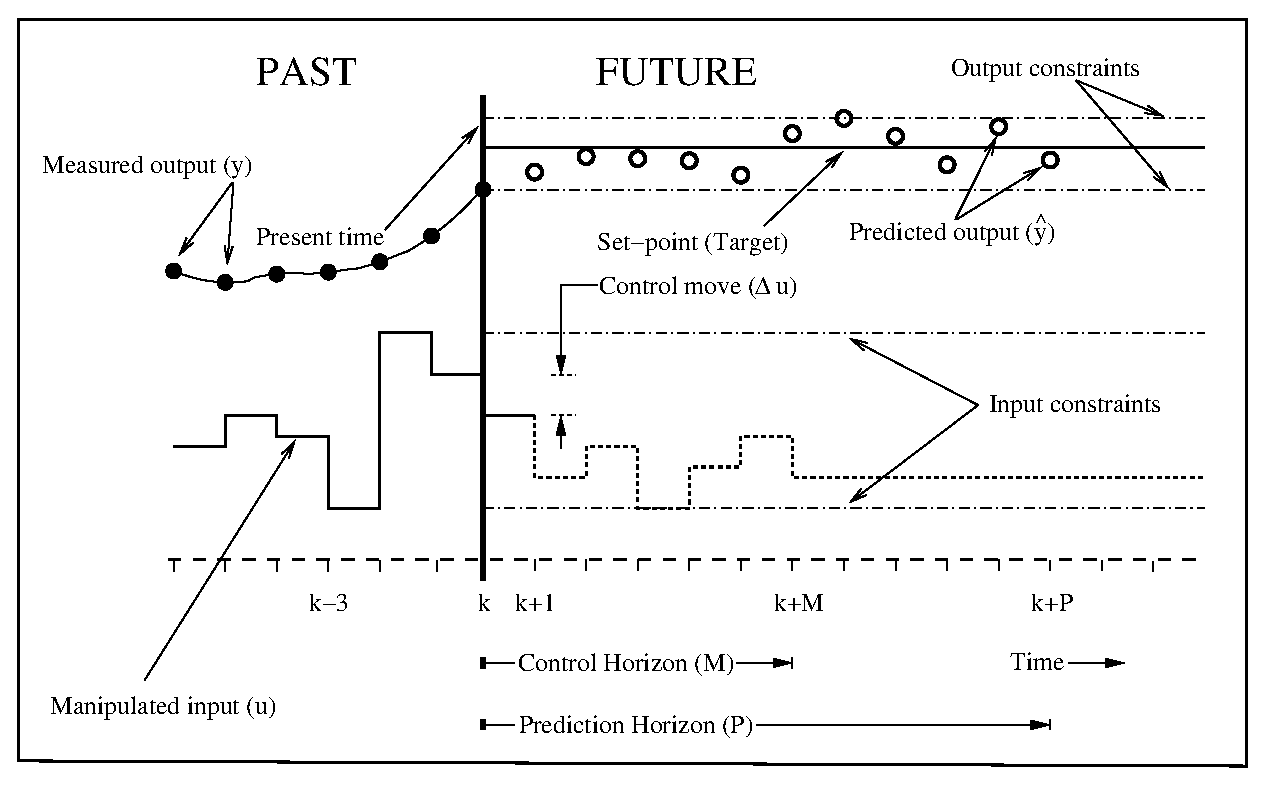
\includegraphics[width=8.2in]{mpc.eps}
% \end{center}
% \caption{Schematic illustrating receding horizon control.
% \label{fig:mpc} }
% \end{figure}
% \end{quote}
% \renewcommand{\baselinestretch}{2}
% \small\normalsize
% \end{landscape}

\begin{landscape}
\renewcommand{\baselinestretch}{1}
\small\normalsize
\begin{quote}
\begin{figure}[!tpb]%figure2
\begin{center}
\includegraphics[width=1.4\textheight]{compression_results.pdf}
\end{center}
\renewcommand{\baselinestretch}{1}
\small\normalsize
%\begin{quote}
\caption[Mean squared error versus bits/base-call for different
  compression methods applied to the \textit{Rhodobacter sphaeroides}
  2.4.1, and \textit{Homo sapiens} chromosome 14 fragment libraries,
  and \textit{Escherichia coli} str. K-12 MG1655, and \textit{Mus
    musculus} datasets]{Mean squared error versus bits/base-call for different
  compression methods applied to the \textit{Rhodobacter sphaeroides}
  2.4.1, and \textit{Homo sapiens} chromosome 14 fragment libraries,
  and \textit{Escherichia coli} str. K-12 MG1655, and \textit{Mus
    musculus} datasets. 2B --- 2-bin encoding; P$n$ --- profiling
  with $n$ profiles; R$n$ --- modeling with polynomial regression
  models of degree $n$; Q$n$ --- \textsc{q}ual\textsc{c}omp with rate parameter of
  $n$. Asterisks denote the corresponding lossless compression using
  \textsc{bz}ip2, with the black asterisk corresponds to original uncompressed
  data.}
  \label{fig:mse_vs_bpbp}
\end{figure}
\end{quote}
\renewcommand{\baselinestretch}{2}
\small\normalsize
\end{landscape}

\subsubsection{Performance evaluation}

As a measure of compression effectiveness we use bits/base-call, and
define it as the size of the compressed representation of quality
values (in bits) divided by the number of quality values represented.
As a measure of information loss we use mean squared error
(\textsc{mse}) as a loss function, and define it as
$\frac{1}{n}\sum_{i=1}^{n}{(Q_i'-Q_i)^2}$, where $n$ is the number of
sequences, $Q_i'$ is the compressed/decompressed quality value, and
$Q_i$ is the original quality value associated with sequence position
$i$.

We evaluate effects of information loss from quality value compression
on quality control steps of read filtering and trimming, which were
performed using Sickle~\cite{sickle}, and make comparison to
uncompressed data.

We evaluate effects of information loss from quality value compression
on \emph{de novo} genome assembly performance using contiguity
statistics, log average read probability
(\textsc{lap})~\cite{Ghodsi:2013hb}, and a collection of
reference-based metrics. The contiguity statistics include N50, which is defined as the median contig
size (the length of largest contig $c$ such that the total size of the
contigs larger than $c$ exceeds half of the assembly size) and corrected N50, which is the recalculated N50 size after the contigs are broken apart at locations of errors. The
\textsc{lap} score can be viewed as a log likelihood score, where a
value closer to 0 is better. We use a script provided by \textsc{gage}
reference-based evaluation to count single nucleotide polymorphisms
(\textsc{snp}s), relocations, translations, and inversions. The
reference-based metrics are normalized by the length of the assembly
to facilitate comparison. For the genome assembly we used software
that makes use quality values in the assembly process:
\textsc{allpaths-lg}~\cite{Gnerre:2011kx} version r50191 with default
settings and 32 threads.

\subsection{Results}

\subsubsection{Compression effectiveness versus information loss}

We compare the \textsc{mse} versus bits/base-call of the
\textit{Rhodobacter sphaeroides} 2.4.1, \textit{Homo sapiens}
chromosome 14, \textit{Escherichia coli} str. K-12 MG1655, and
\textit{Mus musculus} datasets (Figure \ref{fig:mse_vs_bpbp}). We
only include the fragment libraries for the \textit{Rhodobacter
  sphaeroides} 2.4.1, and \textit{Homo sapiens} chromosome 14 data
sets, but the additional short-jump library results are available in
the Supplementary of the submitted manuscript. Storing the uncompressed quality
values requires 1 byte per base-call because they are stored in
\textsc{ascii} format and is denoted by the dotted black asterisk in
the figure. The lossless compression of each dataset using \textsc{bz}ip2
ranges from 2.19 - 3.10 bits/base-call and is denoted by the colored
asterisks on the abscissa. The compression methods tend to cluster
together across the different datasets. Across all datasets, the
0-degree polynomial regression, profile encodings, and \textsc{q}ual\textsc{c}omp have
the lowest bits/base-call.

\textsc{q}ual\textsc{c}omp with the rate parameter set to 100 bits/read has the lowest
\textsc{mse}, but requires 10-15x more storage than the profile
encoding methods for only a 2-3x reduction in \textsc{mse}. When
\textsc{q}ual\textsc{c}omp's rate parameter is set to match the profile encoding
methods, \textsc{q}ual\textsc{c}omp performs slightly worse in terms of \textsc{mse}.
In the \textit{Rhodobacter sphaeroides} 2.4.1 fragment library,
\textsc{q}ual\textsc{c}omp with rate 10 bits/read (0.099 bits/bp) has a \textsc{mse} of
17.29. Using 256-profile encoding requires less storage (0.079
bits/bp) and has a lower \textsc{mse} (11.85).

As the order of the polynomial increases, the bits/base-call increase
and the \textsc{mse} decreases at an exponential rate. The 7th-degree
polynomial regression has the highest bits/base-call and in the
\textit{Mus musculus} dataset, and requires more storage than the
\textsc{ascii} original quality values. A 7th-degree polynomial
requires storing eight floating point values, resulting in 32 bytes
per sequence of quality values. The read length of the \textit{Mus musculus}
dataset is only 26, so the 7th-degree polynomial regression is storing
six more bytes than necessary for lossless encoding the quality data.

\begin{figure}[!htb]%figure2
\begin{center}
\includegraphics[width=4in]{preprocessing_results.pdf}
\end{center}
\renewcommand{\baselinestretch}{1}
\small\normalsize
\begin{quote}
\caption[Preprocessing results of \textit{Rhodobacter sphaeroides}
  2.4.1, and \textit{Homo sapiens} chromosome 14 fragment libraries,
  and \textit{Escherichia coli} str. K-12 MG1655, and \textit{Mus
    musculus} datasets]{Preprocessing results of \textit{Rhodobacter sphaeroides}
  2.4.1, and \textit{Homo sapiens} chromosome 14 fragment libraries,
  and \textit{Escherichia coli} str. K-12 MG1655, and \textit{Mus
    musculus} datasets. Sequences were trimmed using Sickle. The
  total amount of bases filtered by each compression method is
  compared with the amount of bases filtered using the uncompressed
  sequences.}
  \label{fig:preprocessing}
\end{quote}
\end{figure}
\renewcommand{\baselinestretch}{2}
\small\normalsize

\subsubsection{Effects on sequence read preprocessing}

The majority of compression methods retain more base-pairs after
preprocessing than the uncompressed sequences (Figure
\ref{fig:preprocessing}). In general, as a given compression model
increases in complexity, i.e., as the number of profiles, polynomial
degrees, or rate increases, the amount of base-pairs kept approaches
the number base-pairs kept using the uncompressed sequences. The
compression methods on the \textit{Mus musculus} dataset have the
greatest proportion of retained base-pairs compared to the
uncompressed sequences. The \textit{Escherichia coli} str. K-12
MG1655 MiSeq dataset has the smallest range.

The 2-bin approach is the only compression method that results in a
higher number of filtered base-pairs across all datasets. Sickle
uses a sliding window approach to smooth the read quality values before
it trims the sequence based on a specific quality threshold. In the
2-bin approach, there is not an even distribution of values per bin.
In other words, \emph{bad} quality values may range from 0-33, whereas
\emph{good} values may only range from 34-40. Thus, mid-range quality
values that are above the threshold (20 by default) are set below the
quality threshold when compressed, resulting in an increased number of
filtered bases.

The 0-degree polynomial regression results in the highest proportion
of bases kept. If the mean quality value of the read is above
the filtering threshold, then no base-pairs are trimmed. Only
reads that are comprised of mainly low quality values will be
filtered.

It is important to highlight that the even though a compression method
may result in the same number of filtered base-pairs as the
uncompressed sequences, it does not mean the \emph{same} base-pairs
were filtered. The 1st-degree and 5th-degree polynomial regression of
the \textit{Rhodobacter sphaeroides} fragment library filters nearly
as many bases as each other. However, if we examine the specific
reads filtered, the 5th-degree polynomial regression discards
approximately two thirds less reads than the 1st-degree polynomial
regression that are kept by the uncompressed reads (4,640 and
12,066 reads, respectively).

\subsubsection{Effects on genome assembly}

No assembly of the \textit{Rhodobacter sphaeroides} 2.4.1 dataset
outperforms all others in all metrics (Table
\ref{fig:assembly_ranks}).
%The assembly of the \textit{Rhodobacter sphaeroides} 2.4.1 dataset
%using the uncompressed reads outperforms all compression methods in
%terms of \textsc{lap}, NG50, relocations, translations, and
%inversions.
Among the compression methods, the 256-, 64-, 128-profile encoding had
the highest ranks, followed by \textsc{q}ual\textsc{c}omp with rates 10 bits/read, 30
bits/read, 100 bits/read, then 7th-degree polynomial regression,
followed by the \textsc{q}ual\textsc{c}omp with rate 6 bits/read, the 2-bin encoding,
and lastly, the 3rd-degree, 5th-degree, and 0-degree polynomials.

The lossy compression methods largely preserve the contiguity found in
the assembly produced using the reads with unmodified quality
values. All compression methods other than 0-degree polynomial
regression produce an N50 ranging from 3.17--3.22 Mbps (see
Supplementary of manuscript). Despite the similar contiguity statistics,
the different compression methods vary noticeably in the amount of
\textsc{snp}s. The order of polynomial has an inverse relationship
with the amount of \textsc{snp}s detected. The 2-bin and profile
methods detected the least amount of \textsc{snp}s compared to the
reference genome, outperforming the assembly using the original
quality values. A more in-depth evaluation is needed to determine
whether these compression methods are missing actual \textsc{snp}s.

It is important to highlight that using uncompressed reads does not
produce the best assembly in terms of any of the metrics. The
uncompressed reads scores worse than the top overall assembly
(256-profile encoding) in terms of assembled bases, missing reference
bases, N50, \textsc{snp}s, indels $>$5bp, and relocations. The
assembly using uncompressed reads has an error rate of roughly 8.75
errors per 100 kb of assembled sequence, while the 256-profile
encoding has an error rate of 8.02 errors per 100 kb.

In general, the greater the polynomial order, the better overall
assembly; however, the 5th-degree polynomial regression performs
slightly worse than the 3rd-degree polynomial. The respective ranks in
terms of N50 and relocations are fairly distant, which lowers the
overall ranking of the 5th-degree polynomial slightly below that for
3rd-degree polynomial model. The 1st- and 0-degree polynomial
regression methods perform poor in all metrics except assembled bases.
One explanation is that the high error portions of reads are being
marked as high quality, so \textsc{allpaths-lg} is unable to trim or
error correct the sequences. Assembled sequences that overlap maybe
unable to align across the errors at the end of the reads, artificially
inflating the assembled genome size.

Among the different \textsc{q}ual\textsc{c}omp rate parameters, the 10 bits/read rate
ranked highest overall, outperforming the other rate parameters in
terms of corrected N50, least missing reference bases, \textsc{snp}s,
and indels $>$5bp. With the exception of the 6 bits/read rate, the
assemblies decrease in rank with the increase in the rate parameter in
terms of corrected N50, and least missing reference bases. This trend
runs counter to the the decrease in \textsc{mse} of the different
rates.


\begin{figure}[!htb]%figure2
\begin{center}
\includegraphics[width=.8\textwidth]{rhodo_assembly_results.pdf}
\end{center}
\renewcommand{\baselinestretch}{1}
\small\normalsize
\begin{quote}
\caption[Rankings of compression methods based on \textit{Rhodobacter
    sphaeroides} assembly attributes]{Rankings of compression methods based on \textit{Rhodobacter
    sphaeroides} assembly attributes sorted by overall
  rank. Assemblies were constructed using \textsc{allpaths-lg}.
  Rankings above the median value are in cyan, those below the median
  value in magenta.}
  \label{fig:assembly_ranks}
\end{quote}
\end{figure}
\renewcommand{\baselinestretch}{2}
\small\normalsize


\subsubsection{Effects on read mapping}

Certain short read alignment tools use the quality value
information when finding potential alignments. Bowtie2 (version 2.2.3)
was used to evaluate the different decompressed \textsc{fastq}
files. Bowtie2 uses quality values written in the \textsc{fastq} files
when mapping reads against a reference genome. The original
uncompressed and decompressed \textsc{fastq} files were mapped with
Bowtie2 against \textit{Rhodobacter sphaeroides} reference genome. The
generated \textsc{sam} file for each compressing approach were
compared with the uncompressed \textsc{sam} file. The total, shared
and unique proportional numbers of mapped reads are calculated with
respect to the uncompressed \textsc{sam} matches as shown in table
\ref{tab:aligner}. Additionally, to monitor the effect of quality
values on mapping in general, Bowtie2 was adjusted so that the maximum
and minimum mismatch penalty were equivalent to maximum and minimum
quality scores (with parameters: --mp 6,6 and --mp 2,2 respectively).

We evaluate the compression methods using two approaches. In the
first approach, we order the compression methods based on how similar
the alignment results are using the original uncompressed quality values, i.e., the
amount of reads aligned by both the uncompressed and compressed
methods plus the amount of reads unaligned by both methods minus the
amount of reads uniquely aligned by the uncompressed and compression
method. In the second approach, we order the compression methods by
total proportion of aligned reads.

The best compression method in terms of similarity with the
uncompressed reads is \textsc{q}ual\textsc{c}omp with rate 100 bits/read, followed by
\textsc{q}ual\textsc{c}omp with rate 30 bits/read, 256-, and 128-profile encoding, then
2-bin encoding, 64-profile encoding, \textsc{q}ual\textsc{c}omp with rate 10 bits/read,
7th-degree polynomial regression, \textsc{q}ual\textsc{c}omp with rate 6 bits/read, and
finally, 5th-degree through 0-degree polynomial regression.

Ranking the compression methods by overall alignment rate produces an
identical ordering as above. Aside from 0-degree polynomial
regression (83.1\%), all other compression methods have an alignment
rate between 87\% and 86.1\%. The alignment rate of the uncompressed
reads is 87\%.

Most of the compression methods did not vary greatly in terms of the
number of reads that were mapped \emph{only} by the compression
method; however, there is a sizable difference in the amount of reads
that are originally mapped, but unmapped by the compressed methods.
\textsc{q}ual\textsc{c}omp with rate 100 bits/read results in the fewest missing
original read alignments (159). Increasing the regression model
polynomial degree results in a decreasing amount of reads that are
originally mapped, but unmapped by the regression model (40,931 to
1,134 reads for 0-degree and 7th-degree, respectively). There is no
such trend for reads that are mapped only by the regression model.

Setting all bases as minimum quality results in the highest proportion
of mapped reads 88.1\%. Conversely, setting all bases as maximum
quality results in the lowest proportion of mapped reads 72.8\%.


% \begin{table*}[!tbhp]
% \centering
% \caption[]{Quality filtering/trimming for the uncompressed and
%   decompressed \textsc{fastq} files. Numbers correspond to the number
%   of reads that are kept or discarded after applying compression with
%   respect to the original, uncompressed values.}
% \label{tab:quality_control}
% \begin{tabular}{lr|cc|cc|cc|cc|cc}
%  & & \multicolumn{2}{c|}{MaxQual} & \multicolumn{2}{c|}{MinQual} & \multicolumn{2}{c|}{2-bin} & \multicolumn{2}{c|}{Degree 0} & \multicolumn{2}{c}{Degree 1} \\
%  & & kept & discarded & kept & discarded & kept & discarded & kept & discarded & kept & discarded \\
%   \cline{2-12}
% & kept & 883576 &   0 &   0 & 883576 & 871035 & 12541 & 728349 & 155227 & 871510 & 12066 \\
% {\em original} & discarded & 141858 &   0 &   0 & 141858 & 1882 & 139976 & 1475 & 140383 & 9214 & 132644 \\
% \cline{2-12}
%  & proportion & 1.000 & 0.000 & 0.000 & 1.000 & 0.851 & 0.149 & 0.712 & 0.288 & 0.859 & 0.141 \\
% \end{tabular}

% \bigskip

% \begin{tabular}{lr|cc|cc|cc|cc|cc}
%  & & \multicolumn{2}{c|}{Degree 3} & \multicolumn{2}{c|}{Degree 5} & \multicolumn{2}{c|}{Degree 7} & \multicolumn{2}{c|}{Profile (64)} & \multicolumn{2}{c}{Profile (128)} \\
%  & & kept & discarded & kept & discarded & kept & discarded & kept & discarded & kept & discarded \\
% \cline{2-12}
% & kept & 872006 & 11570 & 878936 & 4640 & 877802 & 5774 & 876149 & 7427 & 877513 & 6063 \\
% {\em original}  &  discarded & 10369 & 131489 & 10004 & 131854 & 8821 & 133037 & 15795 & 126063 & 17453 & 124405 \\
% \cline{2-12}
% & proportion & 0.860 & 0.140 & 0.867 & 0.133 & 0.865 & 0.135 & 0.870 & 0.130 & 0.873 & 0.127 \\
% \end{tabular}

% \bigskip

% \begin{tabular}{lr|cc|cc|cc|cc|cc}
% &  & \multicolumn{2}{c|}{Profile (256)} & \multicolumn{2}{c|}{\textsc{q}ual\textsc{c}omp (6)} & \multicolumn{2}{c|}{\textsc{q}ual\textsc{c}omp (10)} & \multicolumn{2}{c|}{\textsc{q}ual\textsc{c}omp (30)} & \multicolumn{2}{c}{\textsc{q}ual\textsc{c}omp (100)} \\
%  & &  kept & discarded & kept & discarded & kept & discarded & kept & discarded & kept & discarded \\
% \cline{2-12}
% & kept & 881215 & 2361 & 878702 & 4874 & 879682 & 3894 & 881948 & 1628 & 881939 & 1637 \\
% {\em original}  & discarded & 15985 & 125873 & 13434 & 128424 & 12855 & 129003 & 10872 & 130986 & 7179 & 134679 \\
% \cline{2-12}
% & proportion & 0.875 & 0.125 & 0.870 & 0.130 & 0.870 & 0.130 & 0.871 & 0.129 & 0.867 & 0.133 \\
% \end{tabular}
% \end{table*}

% \begin{landscape}
% \renewcommand{\baselinestretch}{1}
% \small\normalsize
%
% \renewcommand{\baselinestretch}{2}
% \small\normalsize
% \end{landscape}



\begin{landscape}
\renewcommand{\baselinestretch}{1}
\small\normalsize

\begin{table}[!tbhp]
\centering
\begin{tabular}{lr|cc|cc|cc|cc|cc}
 & & \multicolumn{2}{c|}{MaxQual} & \multicolumn{2}{c|}{MinQual} & \multicolumn{2}{c|}{2-bin} & \multicolumn{2}{c|}{Degree 0} & \multicolumn{2}{c}{Degree 1} \\
& & mapped & unmapped & mapped & unmapped & mapped & unmapped & mapped & unmapped & mapped & unmapped \\
\cline{2-12}
& mapped & 746716 & 145897 & 892613 &   0 & 891864 & 749 & 851682 & 40931 & 883390 & 9223 \\
{\em original} & unmapped &   0 & 132821 & 10821 & 122000 & 186 & 132635 &  67 & 132754 &  55 & 132766 \\
\cline{2-12}
%& sum & 746716 & 278718 & 903434 & 122000 & 892050 & 133384 & 851749 & 173685 & 883445 & 141989 \\
& proportion & 0.728 & 0.272 & 0.881 & 0.119 & 0.870 & 0.130 & 0.831 & 0.169 & 0.862 & 0.138 \\
\end{tabular}

\bigskip

\begin{tabular}{lr|cc|cc|cc|cc|cc}
 & & \multicolumn{2}{c|}{Degree 3} & \multicolumn{2}{c|}{Degree 5} & \multicolumn{2}{c|}{Degree 7} & \multicolumn{2}{c|}{Profile (64)} & \multicolumn{2}{c}{Profile (128)} \\
& & mapped & unmapped & mapped & unmapped & mapped & unmapped & mapped & unmapped & mapped & unmapped \\
\cline{2-12}
& mapped & 889537 & 3076 & 891019 & 1594 & 891479 & 1134 & 891753 & 860 & 891952 & 661 \\
{\em original} & unmapped & 117 & 132704 & 155 & 132666 & 154 & 132667 & 144 & 132677 & 143 & 132678 \\
\cline{2-12}
%& sum & 889654 & 135780 & 891174 & 134260 & 891633 & 133801 & 891897 & 133537 & 892095 & 133339 \\
& proportion & 0.868 & 0.132 & 0.869 & 0.131 & 0.870 & 0.130 & 0.870 & 0.130 & 0.870 & 0.130 \\
\end{tabular}

\bigskip

\begin{tabular}{lr|cc|cc|cc|cc|cc}
&  & \multicolumn{2}{c|}{Profile (256)} & \multicolumn{2}{c|}{\textsc{q}ual\textsc{c}omp (6)} & \multicolumn{2}{c|}{\textsc{q}ual\textsc{c}omp (10)} & \multicolumn{2}{c|}{\textsc{q}ual\textsc{c}omp (30)} & \multicolumn{2}{c}{\textsc{q}ual\textsc{c}omp (100)} \\
& &  mapped & unmapped & mapped & unmapped & mapped & unmapped & mapped & unmapped & mapped & unmapped \\
\cline{2-12}
& mapped & 892051 & 562 & 891375 & 1238 & 891777 & 836 & 892233 & 380 & 892454 & 159 \\
{\em original}  & unmapped & 119 & 132702 & 304 & 132517 & 265 & 132556 & 220 & 132601 & 172 & 132649 \\
\cline{2-12}
%& sum & 892170 & 133264 & 891679 & 133755 & 892042 & 133392 & 892453 & 132981 & 892626 & 132808 \\
& proportion & 0.870 & 0.130 & 0.870 & 0.130 & 0.870 & 0.130 & 0.870 & 0.130 & 0.870 & 0.130 \\

\end{tabular}

\caption[Mapping results of decompressed \textsc{fastq} files
  against \textit{Rhodobacter sphaeroides} reference genome]{Mapping results of decompressed \textsc{fastq} files
  against \textit{Rhodobacter sphaeroides} reference genome using
  Bowtie2. Numbers corresponds to the proportion of mapped reads with
  respect to the uncompressed \textsc{fastq}. ``Shared'' denotes the
  percentage of mapped reads by both the uncompressed and decompressed
  data. ``Uncompressed only'' denotes the percentage of reads mapped
  from the uncompressed data that are not mapped after
  decompression. ``Compressed only'' denotes the percentage of reads
  mapped from the decompressed data that were not mapped before
  compression.}

\label{tab:aligner}
\end{table}

\renewcommand{\baselinestretch}{2}
\small\normalsize
\end{landscape}


\subsection{Discussion}

\subsubsection{Lossy compression acceptable for subsequent biological analyses}

The primary concern of using lossy compression methods is naturally
the extent of information loss, that we quantified by \textsc{mse} in
this study. \textsc{mse} and compressibility provide information in
the theoretical context to the methods, but they are not the end-all
of evaluation criteria. The performance of compressed datasets in
different subsequent analyses and applications are just as
important. Our benchmarks showed that some of the compression methods
with high error rates are still practical for certain kinds of
applications. Many subsequent tools proved to have enough additional
redundancy built-in to handle such loss in information. Passing the
decompressed quality values through quality control software shows
that most methods filter nearly as many bases as using original
quality sequences. Assemblers performing sequence alignment use
percent similarity scores that are typically robust to standard
sequencing errors.

\subsubsection{Extension of 2-bin encoding}

2-bin encoding has the nice property of being simple to compute and
has good bits/base-call values. The 2-bin encoding suffers from having
a high \textsc{mse}, but fortunately, we have shown that in the case
of genome assembly, 2-bin encoding outperforms all polynomial
regressions encodings with degree less than 3. 2-bin encoding of the
fragment and short-jump libraries of \textit{Rhodobacter sphaeroides}
have \textsc{mse}s of $2.42\times$ and $10.76\times$ the 3rd-degree
polynomial regression encodings, respectively. This further highlights
the importance of using additional contextual information of the
subsequent analyses when evaluating compressed quality values.

A potential extension to 2-bin encoding is to incorporate an
additional bin (\emph{okay}). The \emph{okay} value can be used where
the base qualities fall within a 2-bin range. Because the distribution
of quality values is skewed towards higher quality, we need to
experiment with different cutoffs for the \emph{okay} value and
determine if the additional storage is noticeable in subsequent
analyses.

\subsubsection{Extension of polynomial regression}

The downside of modeling quality sequences using polynomial regression is that the model often requires a high number of degrees to achieve the same \textsc{mse} as the profile and \textsc{QualComp} methods.
However, storing a high number of coefficients requires more storage than losslessly compressing the original data.
In order to increase the compressibility of modeling, we can attempt to store the \emph{profiles} of certain polynomial functions.
In other words, we can use a spline (a function that is piecewise-defined by polynomial functions) to represent a given quality sequence.
Similar to our profile-encoding method, the user can specify how many polynomial functions they wish to store.
Then a quality sequence can be divided evenly into a given number of segments, and each segment can be annotated with a polynomial function profile that closely matches its quality sequence.

\subsubsection{Potential for operations on compressed data}

Perhaps one of the greatest potential benefits of compressing quality
values is the potential to perform quality control and possibly other
operations directly on the compressed representations of the
data. This is easiest to to consider for profile-based
compression. The $k$ profiles can be evaluated for (pre-)processing
operations such as filtering and trimming, and the operations
transitively applied to the entire set of reads, thus saving
substantial computation associated with evaluating the full set of
reads.

\subsubsection{Future of lossy compression in bioinformatics analyses}

We have simply provided here the initial steps in analyzing the effect
of lossy compression on quality values using a single,
high-coverage bacterial dataset. More work needs to be done using
additional biological datasets, such as human and mouse, along with
different sequencing technologies. A more direct comparison against
related lossy compression tools, such as
\textsc{SlimGene}~\cite{Kozanitis:2011kl} and
\textsc{\textsc{q}ual\textsc{c}omp}~\cite{Ochoa:2013rt}, needs to be
performed. Additionally, other types of sequencing data can be
analyzed apart from the Illumina data examined here. For example, the
PacBio sequencing instruments produce very long reads (with average
read lengths on the order of 10 kbp), but with the trade-off of having
a high error-rate ($\sim$15\%). Unlike the class of quality values we
have examined here, the distribution of erroneous bases is relatively
uniform~\cite{Ferrarini:2013vf}. The assembly complexity of bacterial
genomes can be greatly simplified, producing near complete genome
assemblies, by utilizing a single run of these long
reads~\cite{Koren:2013ye}. If long read sequencing technologies such
as PacBio become more widely adopted, it would be of huge benefit to
examine the potential of lossy compression algorithms on not only the
quality values, but the biological sequencing data themselves.


%%%%%%%%%%%%%%%%%%%%%%%%%%%%%%%%%%%%%%%%%%%%%%%%%%%%%%%%%%%%%%%%%%%%%%%%%%%%%%%%%%%%%
%
%     please remove the " % " symbol from \centerline{\includegraphics{fig01.eps}}
%     as it may ignore the figures.
%
%%%%%%%%%%%%%%%%%%%%%%%%%%%%%%%%%%%%%%%%%%%%%%%%%%%%%%%%%%%%%%%%%%%%%%%%%%%%%%%%%%%%%%

\subsection{Conclusion}

In this paper we have examined lossy compression on sequence quality
values and their effect on subsequent analyses. Although most previous
examinations on lossy compression primarily focused on information
loss, we have shown that typically used bioinformatics software today
have additional built-in sensitivity to handle significant loss of
information in the compressed quality values.
%
% \section*{Acknowledgement}
% We thank the 2014 Bioinformatics
% Exchange for Students and Teachers (\textsc{best}) Summer School,
% funded by the offices of the Dean of The Graduate School at University
% of Maryland and the Rektor of University of T\"{u}bingen, where this
% research was initiated.

\section{K-mulus: Strategies for BLAST in the Cloud}
\subsection{Abstract}
With the increased availability of next-generation sequencing technologies, researchers are gathering more data than they are able to process and analyze. One of the most widely performed analysis is identifying regions of similarity between DNA or protein sequences using the Basic Local Alignment Search Tool, or BLAST. Due to the large amount of sequencing data produced, parallel implementations of BLAST are needed to process the data in a timely manner.  While these implementations have been designed for those researchers with access to computing grids, recent web-based services, such as Amazon's Elastic Compute Cloud, now offer scalable, pay-as-you-go computing.  In this paper, we present K-mulus, an application that performs distributed BLAST queries via Hadoop MapReduce using a collection of established parallelization strategies. In addition, we provide a method to speedup BLAST by clustering the sequence database to reduce the search space for a given query.  Our results show that users must take into account the size of the BLAST database and memory of the underlying hardware to efficiently carry out the BLAST queries in parallel.  Finally, we show that while our database clustering and indexing approach offers a significant theoretical speedup, in practice the distribution of protein sequences prevents this potential from being realized.

%
%\input{subsection_introduction.tex}
\subsection{Introduction}
Identifying regions of similarity between DNA or protein sequences is one of the most widely studied problems in bioinformatics. These similarities can be the result of functional, structural, or evolutionary relationships between the sequences. As a result, many tools have been developed with the intention of efficiently searching for these similarities \cite{altschul1990basic,eddy2009new,kent2002blat}. The most widely used application is the Basic Local Alignment Search Tool, or BLAST\cite{altschul1990basic}.

With the increased availability of next-generation sequencing technologies, researchers are gathering more data than ever before. This large influx of data has become a major issue as researchers have a difficult time processing and analyzing it. For this reason, optimizing the performance of BLAST and developing new alignment tools has been a well researched topic over the past few years. Take the example of environmental sequencing projects, in which the biodiversity of various environments, including the human microbiome, is analyzed and characterized to generate on the order of several terabytes of data\cite{peterson2009nih}. One common way in which biologists use these massive quantities of data is by running BLAST on large sets of unprocessed, repetitive reads to identify putative genes\cite{li2010est,murray2002identification}. Unfortunately, performing this task in a timely manner while dealing with terabytes of data far exceeds the capabilities of most existing BLAST implementations.

As a result of this trend, large sequencing projects require the utilization of high-performance and distributed systems.
BLAST implementations have been created for popular distributed platforms such as Condor\cite{condor-hunter} and MPI\cite{darling2003design,dongarra1993proposal}.
%\emph{mpiBLAST}\cite{darling2003design} is a widely-used distributed version of BLAST, which can yield super-linear speed-up over running BLAST on a single node. \emph{mpiBLAST} works by segmenting the database into equal-sized chunks and distributing these chunks among the available nodes. All nodes then proceed to search the entirety of the query set against all chunks of the database. The results from individual nodes are later aggregated.
Recently, MapReduce\cite{dean2008mapreduce} has become one of the de-facto standards for distributed processing.
There are a few advantages of using the MapReduce framework over other existing parallel processing frameworks. The entirety of the framework rests in two simple methods: a \emph{map} and a \emph{reduce} function.
The underlying framework takes care of the communication between nodes in the cluster.
By abstracting the communication between nodes, it allows software developers to quickly design software that can run in parallel over potentially thousands of processors.
Although this makes it simple to program, without direct control of the communication, it may be more inefficient compared to other distributed platforms.
%For instance, if a developer wanted to count the number of occurrences of each of the words in a body of text, they could design a MapReduce application that would do this in parallel with little to no effort. Initially, they would feed the body of text as the input. Individual words from the file would be distributed evenly among all available nodes. The mappers would output key-value pairs of the form (word, 1). Finally, when all mappers have finished, the reducers will each get a key, and a list of values. In this case, the list of values is exclusively composed of 1s. The reducer would then aggregate all the entries in the list, and output the final key-value pair, which corresponds to (word, count).

%//MOVE to methods/ADD other hadoop Blast implementations.

%CloudBLAST\cite{matsunaga2008cloudblast} is a parallel implementation of BLAST which uses the MapReduce paradigm in conjunction with the Hadoop Distributed File System (HDFS) \cite{borthakur2007hadoop}. Unlike \emph{mpiBLAST}, which speedups up BLAST by segmenting the database, CloudBLAST’s parallelization approach solely involves segmenting the queries.

While these parallel implementations of BLAST were designed to work on large computing grids, most researchers do not have access to these types of clusters, due to their high cost and maintenance requirements.
Fortunately, cloud computing offers a solution to this problem, allowing researchers to run their jobs on demand without the need of owning or managing any large infrastructure.
%//REMOVE: The speedup offered by running large jobs in parallel, as well as the opportunities for novel reduction of the BLAST protein search space\cite{morgulis2008database,williams1996indexing}, are the motivating factors that led us to devote this paper to effectively parallelizing protein BLAST (blastx and blastp).
Web-based services, such as Amazon’s Elastic Compute Cloud (EC2)\cite{inc_amazon_2008}, have risen in recent years to address the need for scalable, pay-as-you-go computing.
These services allow users to select from a collection of pre-configured disk images and services, and also allow more fine-grained customization down to the number of CPUs, speed, and amount of memory in their rented cluster.
%Arguably the most popular, Amazon’s Elastic Compute Cloud (EC2)\cite{inc_amazon_2008} allows users to select pre-configured disk images and services.

In this paper, we present K-mulus, a collection of Hadoop MapReduce tools for performing distributed BLAST queries.
We show that a limitation to previous cloud BLAST implementations is their ``one size fits all'' solution to parallelizing BLAST queries.
We provide several different strategies for parallelizing BLAST depending on the underlying cloud architecture and sequencing data, including: (1) parallelizing on the input queries, (2) parallelizing on the database, and then a (3) hybrid, query and database parallelization approach.
Finally, we describe a k-mer indexing heuristic to achieve speedups by generating database clusters which results in a reduction of the search space during query execution.

%After the database is partitioned by cluster, a lightweight k-mer index is generated for each partition. During a query, the k-mers of the query sequences can be quickly compared against these indices to determine if the cluster contains potential matches. In this way, a query sequence need only be compared against a subset of the original database, thereby reducing the search space.


%\input{subsection_methods.tex}
\subsection{Methods}

%\emph{mpiBLAST}\cite{darling2003design}  Although K-mulus and mpiBLAST’s both divide the database into smaller chunks, mpiBLAST chunks the data arbitrarily, while K-mulus does so according to similarity-based clustering.

\subsubsection{MapReduce}
The MapReduce framework was created by Google to support large-scale parallel execution of data intensive applications using commodity hardware\cite{dean2008mapreduce}.
Unlike other parallel programming framework where developers must explicitly handle inter-process communication, MapReduce developers only have to focus on two major functions, called \emph{map} and \emph{reduce}.

Prior to running a MapReduce program, the data must be first stored in the Hadoop Distributed File System (HDFS).
The user then specifies a \emph{map} function that will run on the chunks of the input data in parallel.
MapReduce is ``data aware,'' performing computation at the nodes containing the required data instead of transferring the data across the network.
The \emph{map} function processes the input in a particular way according to the developer’s specifications, and outputs a series of key-value pairs. Once all nodes have finished outputting their key-value pairs, all the values for a given key are aggregated into a list (via Hadoop's internal shuffle and sort mechanisms), and sent to the assigned reducer. During the reduce phase, the (key, list of values) pairs are processed. This list of values is used to compute the final result according to the application’s needs.
For more details and examples, please see \cite{dean2008mapreduce}.
%For instance, if a developer wanted to count the number of occurrences of each of the words in a body of text, they could design a MapReduce application that would do this in parallel with little to no effort. Initially, they would feed the body of text as the input. Blocks of text from the input file would be distributed evenly among all available nodes.
%During the mapping phase, a mapper would process the text line-by-line.
%Even though each mapper node is assigned a block of a text, the \emph{map} function is called separately on each line of the text.
%The \emph{map} function would split the line by whitespace and for each word, it would output key-value pairs of the form (\emph{word}, 1). Finally, when all mappers have finished, the reducers will each receive a key, and a list of values. In this case, the list of values is exclusively composed of 1's. The reducer would then sum all the entries in the list, and output the final key-value pair, which corresponds to (\emph{word}, count).

\subsubsection{Parallelization Strategies}

\begin{figure}[!htb]%figure2
\begin{center}
\includegraphics[width=0.8\textwidth]{CP112_fig1.pdf}
\end{center}
\renewcommand{\baselinestretch}{1}
\small\normalsize
\begin{quote}
\caption{Query segmentation approach for parallelizing BLAST.}
\label{fig:strategies}
\end{quote}
\end{figure}
\renewcommand{\baselinestretch}{2}
\small\normalsize


K-mulus uses three main strategies to perform distributed BLAST queries using Hadoop MapReduce.
As we will show, the efficacy of these strategies are all dependent on the underlying hardware and data being used.
\subsubsection{Query Segmentation.}
Arguably the simplest way to parallelize an application using MapReduce is to set the \emph{map} function to the given application and execute it on subsets of the input.
The individual results of the \emph{map} functions are then aggregated by a single \emph{reducer}.
This query segmentation is the default implementation of CloudBLAST\cite{matsunaga2008cloudblast}, a popular MapReduce implementation of BLAST.
Instead of writing custom \emph{map} and \emph{reduce} functions, CloudBLAST takes advantage of Hadoop's streaming extension that allows seamless, parallel execution of existing software on Hadoop without having to modify the underlying application.

The first step of the query segmentation approach is to partition the query file into a predetermined number of chunks (usually the number of computing nodes) and send them to random nodes (Fig. \ref{fig:strategies}).
This partitioning of the query sequences can be done automatically as the sequence files are uploaded to the HDFS.
The user must pay special attention to the size of their query sequence file because the block sizes for the HDFS are 128MB by default.
It is possible to underutilize the Hadoop cluster, since the \emph{map} functions are often assigned to blocks of the input data.
If a user uploads a 128MB sequence file to HDFS and uses Hadoop's streaming extension, then despite the number of nodes they request, BLAST will be performed only using the node containing the block of the data.
%K-mulus provides additional functionality to partition the input into the desired number of blocks to prevent this from happening.

During runtime, the \emph{map} function receives as input a block of FASTA-formatted sequences.
Each \emph{map} function simply executes the included BLAST binary against the included database sequences and outputs the results directly to disk.
Although there is no need to use a reducing step for this strategy, one reducer can be used to aggregate the results.
%By using Hadoop, we do not have to worry load balancing and communication between nodes.

\subsubsection{Database Segmentation.}

Instead of segmenting the query, we can segment the database into a predetermined number of chunks.
By segmenting the database, we can reduce the overhead of disk I/O for databases that do not fit completely into memory.
Otherwise, as soon as the database grows larger than the amount of main memory, the runtime increases by orders of magnitude\cite{darling2003design}.
Therefore, it is important to examine the underlying hardware limitations and database size before using the default query segmentation approach.

During runtime, the query sequences are uploaded to the HDFS and sent to all nodes using the DistributedCache feature of Hadoop.  The DistributedCache feature ensures that all nodes involved in the MapReduce have access to the same files.  The \emph{map} function is only responsible for passing the path of the database chunks to the reducer.  Each \emph{reduce} function executes BLAST on the complete set of input sequences.

Since BLAST takes into account the size of the database when computing alignment statistics, the individual BLAST results must have their scores adjusted for the database segmentation.
Fortunately, BLAST provides the user an option to specify the effective length of the complete database.
%In order to determine the k and $\lambda$ values (statistical parameters dependent upon the alignment scoring and the background amino acid frequencies), a test query of one sequence must be performed against against the entire non-segmented database.

\subsubsection{Hybrid Approach.}
One potential problem with the database segmentation approach is that if we evenly partition the database across all nodes in our cluster, then the database chunks may only fill up a small portion of the available memory.
In this case, we must use a hybrid approach, where we segment the database into the least number of chunks that can fit entirely into memory.
%When the database is too large to fit in memory, but segmenting the database results in very small chunks, then we must use a hybrid approach.
Afterwards, we replicate the database chunks across the remaining machines.
During runtime, the query sequences are split and sent to the different the databases chunks, but only sent once to each of the database chunk replicates.
This hybrid approach is also utilized by \emph{mpiBLAST}\cite{darling2003design}, a widely-used distributed version of BLAST using MPI, which can yield super-linear speed-up over running BLAST on a single node.

During runtime, each \emph{map} function receives a chunk of the query sequences and is responsible for sending out the chunk to each database partition.
For each database partition $i$, the \emph{map} function randomly selects a replicate to send the query chunk to in the form of a tuple ($db_{i,\text{replicate\_num}}$, query chunk).
The reducer receives a collection of query chunks for a given database partition and replicate and BLASTs the query chunk against the database partition.

\subsubsection{K-mer Indexing}
One of the original algorithms that BLAST uses is ``seed and extend'' alignment. This approach requires that there be at least one k-mer (sequence sub-string of length k) match between query and database sequence before running the expensive alignment algorithm between them\cite{altschul1990basic}. Using this rule, BLAST can bypass any database sequence which does not share any common k-mers with the query. Using this heuristic, we can design a distributed version of BLAST using the MapReduce model. One aspect of BLAST which we take advantage of is the database indexing of k-mers. While some versions of BLAST have adopted database k-mer indexing for DNA databases, it seems that this approach has not been feasibly scaled to protein databases\cite{morgulis2008database}. For this reason, BLAST iterates through nearly every database sequence to find k-mer hits. Here we describe an approach for K-mulus that attempts to optimize this process by using lightweight database indexing to allow query iteration to bypass certain partitions of the database.

In order to cluster the database, for each sequence, we first create a vector of bits in which the value at each position indicates the presence of a specific sequence k-mer. The index of each k-mer in the vector is trivial to compute.
We then cluster these bit vectors using a collection of clustering algorithms: k-means\cite{hartigan1979algorithm}, and k-medoid\cite{van2003new}.
Our algorithms perform clustering with respect to the presence vectors of each input sequence. For each cluster, a center presence vector is computed as the union of all sequence presence vectors in the cluster. The distance between clusters is taken as the Hamming distance, or number of bitwise differences, between these cluster centers. This design choice creates a tighter correspondence between the clustering algorithm and the metrics for success of the results, which depend entirely on the cluster presence vectors as computed above.
We also keep track of the centers for each cluster as they play the crucial role of identifying membership to a cluster.

After the database has been clustered, we compare the input query sequences to all centers. The key idea is that by comparing the input query sequence to the cluster centers, we can determine whether a potential match is present in a given cluster. If this is the case, we run the BLAST algorithm on the query sequence and the database clusters that we determined as relevant for the query.


%\input{subsection_results.tex}
\subsection{Results}

\subsubsection{Comparison of Parallelization Approaches on a Modest Size Cluster}

\begin{figure}[!htb]%figure2
\begin{center}
\includegraphics[width=0.8\textwidth]{CP112_fig2.pdf}
\end{center}
\renewcommand{\baselinestretch}{1}
\small\normalsize
\begin{quote}
\caption{Runtimes of different BLAST parallelization approaches.}
\label{fig:parallel_approaches}
\end{quote}
\end{figure}
\renewcommand{\baselinestretch}{2}
\small\normalsize


We evaluated the different parallelization approaches of protein BLAST on 30,000 translated protein sequences randomly chosen from the Human Microbiome Project\cite{peterson2009nih} (Fig. \ref{fig:parallel_approaches}).
The sequences were BLAST against NCBI's non-redundant (\emph{nr}) protein database (containing 3,429,135 sequences).
For our analyses we used a 46 node Hadoop (version 0.20.2) cluster.  Each node had 2 map/reduce tasks and 2GB of memory, reproducing a typical cloud cluster.

The \emph{nr} database used was 9GB in size and unable to completely fit into the memory of a single node in our cluster.
We segmented the database into 100 and 500 chunks to test our database segmentation approach.
With 100 database chunks, the database will be roughly split across each reduce task.
We included a partitioning of 500 database chunks to show the effects of over-partitioning the database.

Segmenting the database into 100 and 500 partitions resulted in a 26\% and 16\% decrease in runtime compared to the query segmentation approach, respectively.
Although using a smaller number of database partitions was faster, there are still advantages for using more database partitions.
Assuming an even distribution of query workload, if a node fails near the end of its BLAST execution, then that task must be restarted and the overall runtime is essentially doubled.
Over-partitioning the database allows for a failed task to restart and complete faster.

Our hybrid query and database segmentation approach resulted in a 44\% decrease in runtime compared to only query segmentation.
Considering that the memory of each node in our cluster was 2GB, and the \emph{nr} database was 9GB, we partitioned the database into 5 chunks, each roughly 2GB in size.
This allows the databases to fit completely into memory at each node.

\subsubsection{Analysis of Database k-mer Index}


\begin{figure}[!htb]%figure2
\begin{center}
\includegraphics[width=0.8\textwidth]{CP112_fig3.pdf}
\end{center}
\renewcommand{\baselinestretch}{1}
\small\normalsize
\begin{quote}
\caption{Runtimes of database segmentation with k-mer index approach.}
\label{fig:db_index}
\end{quote}
\end{figure}
\renewcommand{\baselinestretch}{2}
\small\normalsize


Using our clustering and k-mer index approach, we show noticeable speedups on well clustered data.
To demonstrate this we simulated an ideal dataset of 1,000 sequences, where the sequences were composed of one of two disjoint sets of 3-mers.
The database sequences were clustered into two even-size clusters.
The sample query was 10,000 sequences, also comprising one of two disjoint sets of 3-mers.
Figure \ref{fig:db_index} shows the result of running BLAST on the query using Hadoop's streaming extension with query segmentation (the method used by CloudBLAST to execute BLAST queries) and K-mulus.
K-mulus running on 2 cores with 2 databases yields a 56\% decrease in runtime over BLAST using Hadoop's streaming extension on 2 cores.
In practice, this degree of separability is nearly impossible to replicate, but this model allows us to set a practical upper bound for the speedup contributed by clustering and search space reduction.

For a more practical BLAST query using the \emph{nr} database, our database and k-mer indexing approach took 2.75x as long compared to the naive Hadoop streaming method using a realistic query of 30,000 sequences from the HMP project. The poor performance is due to the very high k-mer overlap between clusters and uneven cluster sizes.
Due to the high k-mer overlap, each query sequence is being replicated and compared against nearly all clusters.

K-mulus' database clustering and k-mer indexing approach shows poor performance due entirely to noisy, overlapping clusters. In the worst case, K-mulus will map every query to every cluster and devolve to a naive parallelized BLAST on database segments, while also including some overhead due to database indexing. This is close to the behavior we observed when running our clustering and k-mer index experiments on the \emph{nr} database. In order to describe the best possible clusters we could have generated from a database, we considered a lower limit on the exact k-mer overlap between single sequences in the \emph{nr} database (Fig. \ref{fig:kmer_intersubsection}). We generated this plot by taking 50 random samples of 3000 \emph{nr} sequences each, computing the pairwise k-mer intersubsection between them, and plotting a histogram of the magnitude of pairwise k-mer overlap. This shows that there are very few sequences in the \emph{nr} database which have no k-mer overlap which makes the generation of disjoint clusters impossible. Furthermore, this plot is optimistic in that it does not include BLAST’s neighboring words, nor does it illustrate comparisons against cluster centers which will have intersubsection greater than or equal to that of a single sequence.

One strategy to improve the separability of the clusters and reduce the k-mer intersubsection between clusters is to use repeat masking software.
In order to show the improvement offered by repeat masking, we ran SEG\cite{wootton1993statistics} on the sequences before computing the intersubsection (Fig. \ref{fig:kmer_intersubsection}). On average, SEG resulted in a 6\% reduction in the number of exact k-mer overlap between two given sequences. Repeat masking caused a significant, favorable shift in k-mer intersubsection and would clearly improve clustering results. However, the \emph{nr} database had so much existing k-mer overlap that using SEG preprocessing would have almost no effect on the speed of K-mulus' clustering and k-mer index approach.

\begin{figure}[!htb]%figure2
\begin{center}
\includegraphics[width=0.8\textwidth]{CP112_fig4.pdf}
\end{center}
\renewcommand{\baselinestretch}{1}
\small\normalsize
\begin{quote}
  \caption{Pair-wise k-mer intersubsection of 50 random samples of 3000 original and repeat-masked \emph{nr} sequences.}
  \label{fig:kmer_intersubsection}
\end{quote}
\end{figure}
\renewcommand{\baselinestretch}{2}
\small\normalsize



%\input{subsection_discussion.tex}
\subsection{Discussion}

With Amazon EC2 and other cloud platforms supporting Hadoop, developers should not make assumptions about the underlying hardware.
Here we have provided K-mulus, which gives users the versatility to handle the common ways to perform distributed BLAST queries in the cloud without making assumptions of the underlying hardware and data.
The default approach of most Hadoop implementations of BLAST is to segment the query sequences and run BLAST on the chunks in parallel.
This approach works best when the entire BLAST database can fit into memory of a single machine, but as sequencing becomes cheaper and faster, this will become less likely.
Computing clusters provided by services such as EC2 often contain commodity hardware with low memory, which we have shown makes the default query segmentation approach poor in practice.
The query segmentation approach works quite well on more powerful clusters that are able to load the entire database into memory.
By providing users with the different parallel strategies, they are free to choose the one that is most effective with their data and hardware.

We have also provided a way to speed up BLAST queries by clustering and indexing the database using MapReduce.
The speedup potential is largely dependent on the clusterability of the data.
Protein sequences lie in high-dimensional non-Euclidean space, so by comparing them, we encounter the curse of dimensionality, where almost all pairs of sequences are equally far away from one another.
This problem maybe slightly alleviated if we are trying to cluster multiple datasets of highly redundant sequences (multiple deep coverage whole genome sequencing projects with distinct, non-intersecting k-mer spectra).
Future work includes clustering and indexing the query sequences, which may have higher redundancy than the database sequences.
%Users of NCBI's BLAST web interface are given the option to BLAST their query sequences against non-redundant databases by default, suggesting that non-redundant databases are most often used.
%However, clustering these databases with a stringent enough criteria to get few k-mer intersubsections often results in clusters of very little size\cite{li2002tolerating}.
%When the size of the database clusters are a fraction of the available memory, we have shown that this is quite inefficient.
%One potential improvement is to use a hierarchical clustering algorithm that proceeds until we have enough sequences to fill up the available memory of a node in our cluster.

%Although we focused only on achieving speedups by clustering of the database, it may be worth exploring the potential speedups by clustering the query sequences.
%Unlike the database, which is clustered prior to runtime and used throughout different BLAST executions, the query would have to be clustered at runtime.
%Thus, the efficacy of this approach depends on the speed of the clustering algorithm and k-mer composition of the query sequences.
% to ensure speedups over the default query segmentation approach.

%Our work did not include analysis of any clustering or indexing methods which would have resulted in a loss of BLAST search sensitivity. For example, K-mulus clustering might benefit from the positive results shown for protein k-mer indexing of large k-mers over compressed alphabets\cite{shiryev2007improved}.
%Another possible improvement would be to map queries according to percent k-mer identity to a cluster, or to raise the threshold for required k-mer overlap with a cluster index.
%While these approaches would reduce BLAST sensitivity, the trade off with search speed may be favorable. The motivation for this work comes from our evidence that if protein clustering in K-mulus can be improved, large speedups can be achieved.

Although our clustering and indexing approach was used on protein sequences, the logical next step is to include nucleotide database indexing, which has historically had more success in speeding up sequence alignment\cite{kent2002blat}.
With a four character alphabet and simplified substitution rules, nucleotides are easier to work with than amino acids, and allow for much more efficient hashing by avoiding of the ambiguity inherent in amino acids.
%Furthermore, we expect a more random distribution of nucleotide k-mers than amino acids k-mers, which allows for better clustering.
%While we chose to pursue improvements to protein BLAST,
%In our analysis it has become clear that a K-mulus nucleotide BLAST not only has a promising outlook for a speedup, but could serve as a model for effectively executing the more complex task of protein clustering.

It should be noted that the parallelization strategies presented here would also benefit other commonly used bioinformatics tools.  Short read alignment tools (such as Bowtie2\cite{langmead2012fast}) can be parallelized by partitioning the reference index as well as the query sequences.  More work needs to be done to determine the best parallelization strategies for these tools running on commodity clusters.

% \subsubsubsection{Availability}
% Java source code for K-mulus are located at: \url{https://github.com/biocloud/k-mulus}
%
% \subsubsubsection{Acknowledgments}
% We would like to thank Mohammadreza Ghodsi for advice on clustering, Daniel Sommer for advice on Hadoop, Lee Mendelowitz for manuscript feedback, Katherine Fenstermacher for the name K-mulus, and the other members of the Pop lab for valuable discussions on all aspects of our work.
%
% This work is supported in part by grants from the National Science Foundation, grant IIS-0844494 to MP.

%%%
%% This is file `supertabular.sty',
%% generated with the docstrip utility.
%%
%% The original source files were:
%%
%% supertabular.dtx  (with options: `package')
%% Copyright (C) 1989-2004 Johannes Braams. All rights reserved.
%% 
%% This file was generated from file(s) of the supertabular package.
%% -----------------------------------------------------------------
%% 
%% It may be distributed and/or modified under the
%% conditions of the LaTeX Project Public License, either version 1.3
%% of this license or (at your option) any later version.
%% The latest version of this license is in
%%   http://www.latex-project.org/lppl.txt
%% and version 1.3 or later is part of all distributions of LaTeX
%% version 2003/12/01 or later.
%% 
%% This work has the LPPL maintenance status "maintained".
%% 
%% The Current Maintainer of this work is Johannes Braams.
%% 
%% This file may only be distributed together with a copy of the
%% supertabular package. You may however distribute the supertabular package
%% without such generated files.
%% 
%% The list of all files belonging to the supertabular package is
%% given in the file `manifest.txt.
%% 
%% The list of derived (unpacked) files belonging to the distribution
%% and covered by LPPL is defined by the unpacking scripts (with
%% extension .ins) which are part of the distribution.
%% Sourcefile `supertabular.dtx'.
%%
%% Copyright (C) 1988 by Theo Jurriens
%% Copyright (C) 1990-2004 by Johannes Braams texniek at braams.cistron.nl
%%                            Kersengaarde 33
%%                            2723 BP Zoetermeer NL
%%                       all rights reserved.
%%
%%
\NeedsTeXFormat{LaTeX2e}
\ProvidesPackage{supertabular}
              [2004/02/20 v4.1e the supertabular environment]
\newcount\c@tracingst
\DeclareOption{errorshow}{\c@tracingst\z@}
\DeclareOption{pageshow}{\c@tracingst\tw@}
\DeclareOption{debugshow}{\c@tracingst5\relax}
\ProcessOptions
\newif\if@topcaption \@topcaptiontrue
\def\topcaption{\@topcaptiontrue\tablecaption}
\def\bottomcaption{\@topcaptionfalse\tablecaption}
\long\def\tablecaption{%
  \refstepcounter{table}\@dblarg{\@xtablecaption}}
\long\def\@xtablecaption[#1]#2{%
  \long\gdef\@process@tablecaption{\ST@caption{table}[#1]{#2}}}
\global\let\@process@tablecaption\relax
\newif\ifST@star
\newif\ifST@mp
\newdimen\ST@wd
\newskip\ST@rightskip
\newskip\ST@leftskip
\newskip\ST@parfillskip
\long\def\ST@caption#1[#2]#3{\par%
  \addcontentsline{\csname ext@#1\endcsname}{#1}%
                  {\protect\numberline{%
                      \csname the#1\endcsname}{\ignorespaces #2}}
  \begingroup
    \@parboxrestore
    \normalsize
    \if@topcaption \vskip -10\p@ \fi
    \@makecaption{\csname fnum@#1\endcsname}{\ignorespaces #3}\par
    \if@topcaption \vskip 10\p@ \fi
  \endgroup}
\newcommand\tablehead[1]{%
  \gdef\@tablehead{%
  \noalign{%
      \global\let\@savcr=\\
      \global\let\\=\org@tabularcr}%
    #1%
    \noalign{\global\let\\=\@savcr}}}
\tablehead{}
\newcommand\tablefirsthead[1]{\gdef\@table@first@head{#1}}
\newcommand\tabletail[1]{%
  \gdef\@tabletail{%
    \noalign{%
      \global\let\@savcr=\\
      \global\let\\=\org@tabularcr}%
    #1%
    \noalign{\global\let\\=\@savcr}}}
\tabletail{}
\newcommand\tablelasttail[1]{\gdef\@table@last@tail{#1}}
\newcommand\sttraceon{\c@tracingst5\relax}
\newcommand\sttraceoff{\c@tracingst\z@}
\newcommand\ST@trace[2]{%
  \ifnum\c@tracingst>#1\relax
    \GenericWarning
      {(supertabular)\@spaces\@spaces}
      {Package supertabular: #2}%
  \fi
  }
\newdimen\ST@pageleft
\newcommand*\shrinkheight[1]{%
  \noalign{\global\advance\ST@pageleft-#1\relax}}
\newcommand*\setSTheight[1]{%
  \noalign{\global\ST@pageleft=#1\relax}}
\newdimen\ST@headht
\newdimen\ST@tailht
\newdimen\ST@pagesofar
\newdimen\ST@pboxht
\newdimen\ST@lineht
\newdimen\ST@stretchht
\newdimen\ST@prevht
\newdimen\ST@toadd
\newdimen\ST@dimen
\newbox\ST@pbox
\def\ST@tabularcr{%
  {\ifnum0=`}\fi
  \@ifstar{\ST@xtabularcr}{\ST@xtabularcr}}
\def\ST@xtabularcr{%
  \@ifnextchar[%]
    {\ST@argtabularcr}%
    {\ifnum0=`{\fi}\cr\ST@cr}}
\def\ST@argtabularcr[#1]{%
  \ifnum0=`{\fi}%
  \ifdim #1>\z@
    \unskip\ST@xargarraycr{#1}
  \else
    \ST@yargarraycr{#1}%
  \fi}
\def\ST@xargarraycr#1{%
  \@tempdima #1\advance\@tempdima \dp \@arstrutbox
  \vrule \@height\z@ \@depth\@tempdima \@width\z@ \cr
  \noalign{\global\ST@toadd=#1}\ST@cr}
\def\ST@yargarraycr#1{%
  \cr\noalign{\vskip #1\global\ST@toadd=#1}\ST@cr}
\def\ST@startpbox#1{%
  \setbox\ST@pbox\vtop\bgroup\hsize#1\@arrayparboxrestore}
\def\ST@astartpbox#1{%
  \bgroup\hsize#1%
  \setbox\ST@pbox\vtop\bgroup\hsize#1\@arrayparboxrestore}
\def\ST@endpbox{%
  \@finalstrut\@arstrutbox\par\egroup
  \ST@dimen=\ht\ST@pbox
  \advance\ST@dimen by \dp\ST@pbox
  \ifnum\ST@pboxht<\ST@dimen
    \global\ST@pboxht=\ST@dimen
  \fi
  \ST@dimen=\z@
  \box\ST@pbox\hfil}
\def\ST@aendpbox{%
  \@finalstrut\@arstrutbox\par\egroup
  \ST@dimen=\ht\ST@pbox
  \advance\ST@dimen by \dp\ST@pbox
  \ifnum\ST@pboxht<\ST@dimen
    \global\ST@pboxht=\ST@dimen
  \fi
  \ST@dimen=\z@
  \unvbox\ST@pbox\egroup\hfil}
\def\estimate@lineht{%
  \ST@lineht=\arraystretch \baslineskp
  \global\advance\ST@lineht by 1\p@
  \ST@stretchht\ST@lineht\advance\ST@stretchht-\baslineskp
  \ifdim\ST@stretchht<\z@\ST@stretchht\z@\fi
  \ST@trace\tw@{Average line height: \the\ST@lineht}%
  \ST@trace\tw@{Stretched line height: \the\ST@stretchht}%
  }
\def\@calfirstpageht{%
  \ST@trace\tw@{Calculating height of tabular on first page}%
  \global\ST@pagesofar\pagetotal
  \global\ST@pageleft\@colroom
  \ST@trace\tw@{Height of text = \the\pagetotal; \MessageBreak
                Height of page = \the\ST@pageleft}%
  \if@twocolumn
    \ST@trace\tw@{two column mode}%
    \if@firstcolumn
     \ST@trace\tw@{First column}%
      \ifnum\ST@pagesofar > \ST@pageleft
        \global\ST@pageleft=2\ST@pageleft
        \ifnum\ST@pagesofar > \ST@pageleft
          \newpage\@calnextpageht
          \ST@trace\tw@{starting new page}%
        \else
          \ST@trace\tw@{Second column}%
          \global\advance\ST@pageleft -\ST@pagesofar
          \global\advance\ST@pageleft -\@colroom
        \fi
      \else
        \global\advance\ST@pageleft by -\ST@pagesofar
        \global\ST@pagesofar\z@
      \fi
    \else
      \ST@trace\tw@{Second column}
      \ifnum\ST@pagesofar > \ST@pageleft
        \ST@trace\tw@{starting new page}%
        \newpage\@calnextpageht
      \else
        \global\advance\ST@pageleft by -\ST@pagesofar
        \global\ST@pagesofar\z@
      \fi
    \fi
  \else
    \ST@trace\tw@{one column mode}%
    \ifnum\ST@pagesofar > \ST@pageleft
      \ST@trace\tw@{starting new page}%
      \newpage\@calnextpageht
    \else
      \global\advance\ST@pageleft by -\ST@pagesofar
      \global\ST@pagesofar\z@
    \fi
  \fi
  \ST@trace\tw@{Available height: \the\ST@pageleft}%
  \ifx\@@tablehead\@empty
    \ST@headht=\z@
  \else
    \setbox\@tempboxa=\vbox{\@arrayparboxrestore
      \ST@restore
      \expandafter\tabular\expandafter{\ST@tableformat}%
      \@@tablehead\endtabular}%
    \ST@headht=\ht\@tempboxa\advance\ST@headht\dp\@tempboxa
  \fi
  \ST@trace\tw@{Height of head: \the\ST@headht}%
  \ifx\@tabletail\@empty
    \ST@tailht=\z@
  \else
    \setbox\@tempboxa=\vbox{\@arrayparboxrestore
      \ST@restore
      \expandafter\tabular\expandafter{\ST@tableformat}
        \@tabletail\endtabular}
    \ST@tailht=\ht\@tempboxa\advance\ST@tailht\dp\@tempboxa
  \fi
  \advance\ST@tailht by \ST@lineht
  \ST@trace\tw@{Height of tail: \the\ST@tailht}%
  \ST@trace\tw@{Maximum height of tabular: \the\ST@pageleft}%
  \@tempdima\ST@headht
  \advance\@tempdima\ST@lineht
  \advance\@tempdima\ST@tailht
  \ST@trace\tw@{Minimum height of tabular: \the\@tempdima}%
  \ifnum\@tempdima>\ST@pageleft
    \ST@trace\tw@{starting new page}%
    \newpage\@calnextpageht
  \fi
}
\def\@calnextpageht{%
  \ST@trace\tw@{Calculating height of tabular on next page}%
  \global\ST@pageleft\@colroom
  \global\ST@pagesofar=\z@
  \ST@trace\tw@{Maximum height of tabular: \the\ST@pageleft}%
  }
\def\x@supertabular{%
  \let\org@tabular\tabular
  \let\tabular\inner@tabular
  \expandafter\let
    \csname org@tabular*\expandafter\endcsname
    \csname tabular*\endcsname
  \expandafter\let\csname tabular*\expandafter\endcsname
    \csname inner@tabular*\endcsname
  \if@topcaption \@process@tablecaption \fi
  \global\let\@oldcr=\\
  \def\baslineskp{\baselineskip}%
  \ifx\undefined\@classix
    \let\org@tabularcr\@tabularcr
    \let\@tabularcr\ST@tabularcr
    \let\org@startpbox=\@startpbox
    \let\org@endpbox=\@endpbox
    \let\@@startpbox=\ST@startpbox
    \let\@@endpbox=\ST@endpbox
  \else
    \let\org@tabularcr\@arraycr
    \let\@arraycr\ST@tabularcr
    \let\org@startpbox=\@startpbox
    \let\org@endpbox=\@endpbox
    \let\@startpbox=\ST@astartpbox
    \let\@endpbox=\ST@aendpbox
  \fi
  \ifx\@table@first@head\undefined
    \let\@@tablehead=\@tablehead
  \else
    \let\@@tablehead=\@table@first@head
  \fi
  \let\ST@skippage\ST@skipfirstpart
  \estimate@lineht
  \@calfirstpageht
  \noindent
  }
\def\supertabular{%
  \@ifnextchar[{\@supertabular}%]
               {\@supertabular[]}}
\def\@supertabular[#1]#2{%
  \def\ST@tableformat{#2}%
  \ST@trace\tw@{Starting a new supertabular}%
  \global\ST@starfalse
  \global\ST@mpfalse
  \x@supertabular
  \expandafter\org@tabular\expandafter{\ST@tableformat}%
  \@@tablehead}
\@namedef{supertabular*}#1{%
  \@ifnextchar[{\@nameuse{@supertabular*}{#1}}%
               {\@nameuse{@supertabular*}{#1}[]}%]
  }
\@namedef{@supertabular*}#1[#2]#3{%
  \ST@trace\tw@{Starting a new supertabular*}%
  \def\ST@tableformat{#3}%
  \ST@wd=#1\relax
  \global\ST@startrue
  \global\ST@mpfalse
  \x@supertabular
  \expandafter\csname org@tabular*\expandafter\endcsname
  \expandafter{\expandafter\ST@wd\expandafter}%
  \expandafter{\ST@tableformat}%
  \@@tablehead}%
\def\mpsupertabular{%
  \@ifnextchar[{\@mpsupertabular}%]
               {\@mpsupertabular[]}}
\def\@mpsupertabular[#1]#2{%
  \def\ST@tableformat{#2}%
  \ST@trace\tw@{Starting a new mpsupertabular}%
  \global\ST@starfalse
  \global\ST@mptrue
  \ST@rightskip \rightskip
  \ST@leftskip \leftskip
  \ST@parfillskip \parfillskip
  \x@supertabular
  \minipage{\columnwidth}%
  \parfillskip\ST@parfillskip
  \rightskip \ST@rightskip
  \leftskip \ST@leftskip
  \noindent\expandafter\org@tabular\expandafter{\ST@tableformat}%
  \@@tablehead}
\@namedef{mpsupertabular*}#1{%
  \@ifnextchar[{\@nameuse{@mpsupertabular*}{#1}}%
               {\@nameuse{@mpsupertabular*}{#1}[]}%]
  }
\@namedef{@mpsupertabular*}#1[#2]#3{%
  \ST@trace\tw@{Starting a new mpsupertabular*}%
  \def\ST@tableformat{#3}%
  \ST@wd=#1\relax
  \global\ST@startrue
  \global\ST@mptrue
  \ST@rightskip \rightskip
  \ST@leftskip \leftskip
  \ST@parfillskip \parfillskip
  \x@supertabular
  \minipage{\columnwidth}%
  \parfillskip\ST@parfillskip
  \rightskip \ST@rightskip
  \leftskip \ST@leftskip
  \noindent\expandafter\csname org@tabular*\expandafter\endcsname
  \expandafter{\expandafter\ST@wd\expandafter}%
  \expandafter{\ST@tableformat}%
  \@@tablehead}%
\def\endsupertabular{%
  \ifx\@table@last@tail\undefined
    \@tabletail
  \else
    \@table@last@tail
  \fi
  \csname endtabular\ifST@star*\fi\endcsname
  \ST@restore
  \if@topcaption
  \else
    \@process@tablecaption
    \@topcaptiontrue
  \fi
  \global\let\\\@oldcr
  \global\let\@process@tablecaption\relax
  \ST@trace\tw@{Ended a supertabular\ifST@star*\fi}%
  }
\expandafter\let\csname endsupertabular*\endcsname\endsupertabular
\def\endmpsupertabular{%
  \ifx\@table@last@tail\undefined
    \@tabletail
  \else
    \@table@last@tail
  \fi
  \csname endtabular\ifST@star*\fi\endcsname
  \endminipage
  \ST@restore
  \if@topcaption
  \else
    \@process@tablecaption
    \@topcaptiontrue
  \fi
  \global\let\\\@oldcr
  \global\let\@process@tablecaption\relax
  \ST@trace\tw@{Ended a mpsupertabular\ifST@star*\fi}%
  }
\expandafter\let\csname endmpsupertabular*\endcsname\endmpsupertabular
\def\ST@restore{%
  \ifx\undefined\@classix
    \let\@tabularcr\org@tabularcr
  \else
    \let\@arraycr\org@tabularcr
  \fi
  \let\@startpbox\org@startpbox
  \let\@endpbox\org@endpbox
  }
\def\inner@tabular{%
  \ST@restore
  \let\\\@oldcr
  \noindent
  \org@tabular}
\@namedef{inner@tabular*}{%
  \ST@restore
  \let\\\@oldcr
  \noindent
  \csname org@tabular*\endcsname}
\def\ST@cr{%
  \noalign{%
    \ifnum\ST@pboxht<\ST@lineht
      \global\advance\ST@pageleft -\ST@lineht
      \global\ST@prevht\ST@lineht
    \else
     \ST@trace\thr@@{Added par box with height \the\ST@pboxht}%
      \global\advance\ST@pageleft -\ST@pboxht
      \global\advance\ST@pageleft -0.1\ST@pboxht
      \global\advance\ST@pageleft -\ST@stretchht
      \global\ST@prevht\ST@pboxht
      \global\ST@pboxht\z@
    \fi
    \global\advance\ST@pageleft -\ST@toadd
    \global\ST@toadd=\z@
    \ST@trace\thr@@{Space left for tabular: \the\ST@pageleft}%
  }
  \noalign{\global\let\ST@next\@empty}%
  \ifnum\ST@pageleft<\z@
    \ST@skippage
  \else
    \noalign{\global\@tempdima\ST@tailht
      \global\advance\@tempdima\ST@prevht
    \ifST@mp
      \ifvoid\@mpfootins\else
        \global\advance\@tempdima\ht\@mpfootins
        \global\advance\@tempdima 3pt
      \fi
    \fi}
    \ifnum\ST@pageleft<\@tempdima
      \ST@newpage
    \fi
  \fi
  \ST@next}
\def\ST@skipfirstpart{%
  \noalign{%
    \ST@trace\tw@{Tabular too high, moving to next page}%
    \global\advance\ST@pageleft\pagetotal
    \global\ST@pagesofar\z@
    \newpage
    \global\let\ST@skippage\ST@newpage
    }}
\def\ST@newpage{%
  \noalign{\ST@trace\tw@{Starting new page, writing tail}}%
  \@tabletail
  \ifST@star
    \csname endtabular*\endcsname
  \else
    \endtabular
  \fi
  \ifST@mp
    \endminipage
  \fi
  \global\let\ST@skippage\ST@newpage
  \newpage\@calnextpageht
  \let\ST@next\@tablehead
  \ST@trace\tw@{writing head}%
  \ifST@mp
    \noindent\minipage{\columnwidth}%
    \parfillskip\ST@parfillskip
    \rightskip \ST@rightskip
    \leftskip \ST@leftskip
  \fi
  \noindent
  \ifST@star
    \expandafter\csname org@tabular*\expandafter\endcsname
    \expandafter{\expandafter\ST@wd\expandafter}%
    \expandafter{\ST@tableformat}%
  \else
    \expandafter\org@tabular\expandafter{\ST@tableformat}%
  \fi}
\endinput
%%
%% End of file `supertabular.sty'.

\titleformat{\chapter}
      {\normalfont\large}{Appendix \thechapter:}{1em}{}
%%Appendix -- January 2015
\appendix
\renewcommand{\thechapter}{A}
\renewcommand{\chaptername}{Appendix}

\chapter{Previous Experiments}

The understanding of nonlinear processes in optical fibers is crucial towards 
extending the capabilities of modern optical communication systems based on 
wavelength division multiplexing (WDM), where each communication channel is 
represented by a unique wavelength. One of the nonlinear processes that 
limits the information carrying capacity of a WDM system is four-wave mixing 
(FWM), which causes cross-talk between neighboring channels. This places a 
lower limit on the wavelength separation between adjacent channels and an
upper limit on the input power in each channel. In this study, we describe
a process by which the evolution of FWM processes in an optical fiber can be 
used to estimate the inhomogeneities in the fiber core material, in particular 
the fluctuations in the linear refractive index of the fiber core.  

\section{Overview}

Experiments measuring the evolution of FWM processes along a length of fiber 
were carried out by Hart {\it et al.}\ \cite{hart1} and are described in detail in 
Sec.\ 2.2. In this experiment, two input pump waves at frequencies
$\omega_1$ and $\omega_2$, interacted with each other through the third-order 
nonlinearity of the fiber material to generate first-order sidebands at frequencies 
$\omega_3 = 2\omega_1 - \omega_2$ and $\omega_4 = 2\omega_2 - \omega_1$. 
These waves further interacted to produce second-order sidebands at 
$\omega_5 = 2\omega_3 - \omega_4$ and $\omega_6 = 2\omega_4 - \omega_3$. 
Higher-order sidebands were also generated. The normalized power in the 
sideband at frequency $\omega_m$ was represented by $\rho_m$. The 
evolution of the FWM processes was characterized by the evolution of 
$\rho_m$(z) as a function of fiber length z. 

In the present work, we make a quantitative comparison between these 
experimental results and our numerical results based on efficient algorithms 
\cite{Agrawal2} to solve the nonlinear Schr\"odinger equation (NLSE) that
governs the system. The numerical model, its underlying assumptions and
the results are described in Sec.\ 2.3. A realistic description of a 
standard single mode optical fiber must take into account the random phase 
perturbations a light wave undergoes while propagating through it, without 
disturbing the underlying conservative properties of the system. The NLSE 
needs to be suitably modified in order to incorporate the stochastic nature 
of the propagation. In order to preserve the conservative properties of the 
system, the stochastic terms in the NLSE must necessarily be multiplicative in 
nature as an additive term acts as a source or a sink. An algorithm that 
achieves this with linear, Gaussian, $\delta$-correlated noise is outlined in 
Sec.\ 2.3. This algorithm preserves the unconditional stability of the 
system. At the same time, care is taken to transform the stochastic NLSE from 
its original Ito representation \cite{ito} to the computationally feasible Stratanovich 
representation \cite{stratanovich} by compensating for the 
spurious linear drift that results from integrating such stochastic 
differential equations \cite{risken,werner2,drummond1,carter3}. The dominant 
sources of phase noise are discussed in Sec.\ 2.4. 

Conclusions on the relevance of the experiments of Hart {\it et al.}\ \cite{hart1} 
and the stochastic modeling presented here are summarized in Sec.\ 2.5.    

\section{Experimental and Computational Background}

In this work, we focus on tracing the evolution of the sidebands, generated 
through FWM, along a length of optical fiber. The FWM spectral evolution along
50\,m of fiber for two input pump power regimes (2.1\,W and 5.5\,W) was
investigated \cite{hart1}. In the 2.1\,W case, the sideband evolution followed a damped 
sinusoid along the length of the fiber. The experiments also found that the 
two first-order sidebands ($\rho_3$-blueshifted and $\rho_4$-redshifted from 
the two pumps) had different evolutions along the fiber (with different 
spatial wavelengths). For the 5.5\,W case, the evolution of both first- and 
second-order sidebands was measured. The damping in the first-order sidebands 
($\rho_3$ and $\rho_4$) occured faster than in the 2.1\,W case. Experiments 
probing the dependence of the sideband power on the input power (ranging from 
2\,W to 17\,W) were also performed at a fixed output length of 50\,m of the fiber.
At the same fiber length, the optical spectra for input powers ranging from 
2\,W to 17\,W were also recorded \cite{hart1}. The spectral envelopes were observed to fit 
well to a hyperbolic secant function and the fit parameters were recorded. 
Measurements with a high-resolution wavemeter showed that one of the two pumps 
consisted of two very closely spaced longitudinal modes 
($\Delta\nu\sim$ 0.5\,GHz) which were not resolved by the spectrometer used to 
record the FWM spectra. Inclusion of this multimode nature of the pump input 
in their model was found to alter the sideband dynamics dramatically and 
partly explained the asymmetry between the blue-shifted and red-shifted 
sidebands though it did not account for the damping in the sidebands. This 
was accounted for by adding weak phase fluctuations to the waves as they 
propagated along the fiber \cite{hart1}. The physical source of these phase fluctuations 
was not known at that time. However, the inclusion of the phase fluctuations 
into the model gave excellent qualitative and quantitative agreement with 
experiment. Their model involved integration of a system of coupled ODEs 
derived from the NLSE \cite{thompson1} by a process of truncation that 
retained only the leading frequency components (the pumps and the first- and 
second-order sidebands), a process justified by the fact that the input pump 
waves are well approximated by a combination of monochromatic waves. Their 
final numerical results are based on simulations using the truncated-ODE model
with Langevin noise terms representing phase fluctuations in the fiber. 
Another physical source of stochasticity in their experiment was the inherent 
power fluctuation in the lasers used as the input pumps. The level of 
fluctuations (5-20\%) was measured and incorporated appropriately into their 
model through stochastic initial conditions. This explained the evolution of 
the level of observed fluctuations in the sideband trajectories although it 
was found to be inadequate by itself, to account for the damping of the 
trajectories. They found that all three physical characteristics mentioned 
above, namely the multimode nature of the pump input, the stochastic phase 
fluctuations along the length of the fiber, and the stochastic initial power 
fluctuations were crucial to explaining the different features of the 
experimental measurements \cite{hart1}. 

\section{Stochastic NLSE Model}

In the present work, we have developed and implemented an unconditionally 
stable scheme for integrating the NLSE that successfully incorporates phase 
noise into the SSFM. Thus, we are now in a position to harness the high 
frequency / time resolution of the SSFM together with its efficient 
convergence properties. Due to these advances, we are now able to do 
simulations with much higher frequency resolution (60\,MHz as compared to 
300\,GHz in the ODE model). This high resolution, coupled with an appropriate 
convolution scheme, enables us to compare these simulated spectra with the 
composite spectra observed by the spectrometers which had a resolution of 
$\sim$ 60\,GHz. This was not possible with the truncated ODE model as the 
resolution of the simulated spectra in that case was $\sim$ 300\,GHz. For 
exactly the same levels of phase fluctuations, and initial condition 
fluctuations as used in Ref.\ \cite{hart1}, comparisons for the present NLSE 
model with the experimental sideband evolution functions $\rho_i(z)$ show 
excellent quantitative agreement. These results, along with the algorithms 
employed, are described in detail in this section. We have identified linear 
refractive index fluctuations along the fiber length to be a strong candidate 
for a physical source of the stochastic phase fluctuations. A comparison 
between the various possible sources is given in Sec.\ 2.4.

Under the assumption that the electric field of the light in the fiber has a 
slowly varying envelope $A(z,\tau)$, and that the fiber medium has an 
instantaneous nonlinear response, the system is well described by the 
nonlinear Schr\"{o}dinger equation (NLSE) with a linear multiplicative
stochastic term
%A.1
\begin{equation}
{\partial U \over \partial z} + {i\beta^{(2)} \over 2T_0^2} 
{\partial^2 U \over \partial\tau^2} + {\alpha U \over 2}
 + i\Gamma(z,\tau)U-i\gamma P_0 |U|^2 U = 0.
\end{equation}
$Z$ is distance along the length of the fiber, 
$U(z,\tau)=A(z,\tau)/\sqrt{P_0}$ is the complex electric field envelope 
$A(z,\tau)$ normalized to the absolute amplitude of the field $\sqrt{P_0}$, 
$P_0$ is the total power in the fiber, $\tau$ is time normalized to a 
convenient time scale $T_0(\sim 1\ ns)$ measured in a reference frame 
moving with the group velocity of the pulse [$\tau=(t-z/v_g)/T_0$]. The 
simulations are carried out for exactly the same physical parameters as the 
experiments and simulations reported by Hart {\it et al}.\ \cite{hart1}, i.e., 
$\beta^{(2)}=55\,(ps)^2/km$, is the group velocity dispersion of the fiber at 
the operating wavelength $\lambda_{0}\sim$ 632\,nm 
($k_0\sim 10^7\,m^{-1}$). A loss of $\sim$ 6\,dB/km gives $\alpha$ = 0.0014\,m$^{-1}$ as the 
loss in the fiber at this wavelength. The nonlinearity coefficient 
$\gamma=0.019\,W^{-1}m^{-1}$ is given by 
%A.2
\begin{equation}
\gamma = {\omega_{ave}n_2^I \over cA_{eff}},
\end{equation}
where $A_{eff}$ is the effective core area of the fiber,
$n_2^I$ is the Kerr coefficient for the intensity-dependent refractive index, and 
$\omega_{ave}$ is the average angular frequency of the wave envelope. 
$\Gamma(z,\tau)$ is a linear multiplicative phase noise field. In this study 
the noise field is assumed to be $\delta$-correlated in both space and time. 
The evolution of the FWM dynamics is found to be sensitive to the strength of 
this noise field. It can be physically interpreted as phase noise arising due 
to fluctuations in the linear refractive index of the fiber medium. A detailed 
discussion of its physical origin is given in Sec.\ 2.4.

The system was simulated using the Split-Step Fourier Method (SSFM) 
\cite{Agrawal2}. An algorithm for appropriately incorporating stochastic
phase fluctuations along the length of the fiber in the SSFM was developed
and is summarized below.

The NLSE is composed of linear and nonlinear terms, and can be written in operator form as
%A.3
\begin{eqnarray}
{\partial U \over \partial z} & = & (\hat{D}+\hat{S}+\hat{N})U \nonumber \\
\hat{D}& = & {-i\beta^{(2)} \over 2T_0^2}
{\partial^2 \over \partial\tau^2} - {\alpha \over 2} \nonumber \\
\hat{S} & = & i\Gamma(z,\tau) \nonumber \\
\hat{N} & = & i\gamma P_0|U|^2,
\end{eqnarray}
where $\hat{D}$, $\hat{S}$ and $\hat{N}$ are linear
(dispersive), nonlinear 
and stochastic operators, respectively. It has an exact solution for 
infinitesimal $\Delta z$ given by - 
%A.4
\begin{equation}
U(z + \Delta z,\tau) = exp[\Delta z(\hat{D} + \hat{S} + \hat{N})]U(z,\tau) ,
\end{equation}
which can be approximated by
%A.5
\begin{equation}
U(z + \Delta z,\tau) \approx exp[\Delta z \hat{D}]exp[\Delta z \hat{S}]exp[\Delta z \hat{N}]U(z,\tau) .
\end{equation}

The execution of $exp[\Delta z \hat{N}]$ is carried out in $\tau$-space:
%A.6
\begin{equation}
B_1(z,\tau)=exp[\Delta z \hat{N}]U(z,\tau) .
\end{equation}

The execution of $exp[\Delta z \hat{S}]$ and $exp[\Delta z \hat{D}]$ is 
carried out in $\omega$-space.

In particular, the stochastic phase fluctuations are introduced by modifying 
the phase $\phi_j$ of each frequency component $\omega_j$ of the complex 
field according to
%A.7
\begin{eqnarray}
B_2(z,\omega) & = & {\cal{F}}[B_1(z,\tau)] \nonumber \\
B_3(z,\omega_{j}) & = & exp[i \delta\phi(z,\omega_j)]B_2(z,\omega_j) ,
\end{eqnarray}
where $\cal{F}$ represents the Fourier transform operation.

This process only modifies the phase of each complex frequency component, 
leaving its absolute value unchanged. Thus the algorithm conserves the total 
power and the unconditional stability of the system.

The stochastic phase fluctuations $\delta\phi(z,\omega_j)$ are taken to be 
$\delta$-correlated in frequency as well as spatially along the fiber length. 
The Box-Muller algorithm \cite{boxmuller} was used to generate Gaussian random
deviates from computer-generated uniform random deviates $r_{1j}$ and $r_{2j}$
at each spatial step and for each frequency component $\omega_j$. The 
fluctuations are given by
%A.8
\begin{equation}
\delta\phi(z,\omega_{j}) = \sqrt{-2\sigma_{\phi}^2 \Delta z ln(r_{1j})}cos(2 \pi r_{2j}) .
\end{equation}

This is followed by the execution of $exp[\Delta z \hat{D}]$, which is also 
carried out in Fourier space, followed by the inverse transform
%A.9
\begin{equation}
U(z + \Delta z,\tau) = {\cal{F}}^{-1}[exp[\Delta z \hat{D}(i\omega)]B_{3}(z,\omega)] .
\end{equation}

$\hat{D}(i\omega)$ is obtained by replacing $(\partial / \partial \tau)$ 
by $i \omega$.

%Figure A.1
\begin{figure}
\begin{center}
\includegraphics[0in,0in][3.25in,4.266in]{nlsetime.eps}
\end{center}
\renewcommand{\baselinestretch}{1}
\small\normalsize
\begin{quote}
\caption{Multimode pulse input to the NLSE: (a) input pulse in time
domain and (b) input spectrum.}
\label{figA.1}
\end{quote}
\end{figure}
\renewcommand{\baselinestretch}{2}
\small\normalsize

The basic form of the initial complex wave envelope function is 
%A.10
\begin {equation}
U(0,\tau) = exp \left( - {\tau^2 \over 2\tau_p^2} \right)
\left\{ 
\begin{array}{l}
exp\left( {i\Omega\tau \over 2} \right) + \\
exp\left( - {i\Omega\tau \over 2} \right)
\end{array}
\right\} ,
\end{equation}
where $\tau_p$ is the pulse width T$_p$ =5\,ns FWHM, normalized to the time scale 
T$_0$, $\Omega$=366\,GHz is the frequency detuning between the two laser 
sources normalized to a frequency scale $\Omega_0$ = 62.5\,MHz.  Figure A.1(a) 
shows a plot of this pulse $|U(0,\tau)|^2$. The overall Gaussian envelope 
has an FWHM of 5\,ns, the closely spaced dark lines are due to the 366\,GHz 
($\sim$3\,ps) beating between the two input pump frequencies. The 2\,ns 
modulations on the pulse are due to the 0.5\,GHz mode-structure in the 
blue-shifted pump wave. Figure A.1(b) shows the input spectrum of this pulse 
which consists of two highly monochromatic pump waves with a detuning of 
$\Omega$=366\,GHz. The spectrum of the blue-shifted pump, upon magnification, 
is seen to be composed of two very closely spaced peaks, with a separation of 
$\Delta\nu$=0.5\,GHz. Hart {\it et al}.\ \cite{hart1} did not use pulsed 
wave functions in their NLSE simulations as the size of the FFT required to do 
so made it computationally prohibitive at that time. The size of the FFT was 
chosen such that it would accommodate a time span of 16\,ns in order to go 
sufficiently far into the wings on the Gaussian pulse; and a frequency span of 
16\,THz in order to accommodate all the sidebands generated and prevent 
spurious effects due to the reflection boundary conditions implicit in the 
SSFM algorithm. These considerations dictated the size of the FFT to be 
$\geq$(16 THz)$\cdot$(16 ns) = 256000. The nearest power of 2 is 
2$^{18} = 262144$, which has been used throughout the present work. The 
incorporation of the pulsed nature of the light was found to be necessary in 
explaining the dynamics. From the perspective of the coupled amplitude 
equations used by Hart {\it et al}.\ \cite{hart1}, the present model is equivalent 
to a coupled-ODE model with $2^{18}$ coupled ODEs. 

%Figure A.2
\begin{figure}
\begin{center}
\includegraphics[0in,0in][6in,4.572in]{modestruc21ornot.eps}
\end{center}
\renewcommand{\baselinestretch}{1}
\small\normalsize
\begin{quote}
\caption[Short caption for Figure A.2.]
{Effects of inclusion of the multimode nature ($\Delta\nu = 0.5$\,GHz) of the blue-shifted input pump laser on the 1st order sideband evolution as a function of fiber length for P$_0 = 2.1$\,W. Dashed curves represent simulations without the multimode nature and solid curves represent simulations with the multimode nature. $\Omega = 366$\,GHz, $\gamma = 0.019$\,W$^{-1}$\,m$^{-1}$, and $\beta^{(2)} = 55$\,ps$^2$/km (a) power in the blue-shifted sideband, (b) power in the red-shifted sideband.}
\label{figA.2}
\end{quote}
\end{figure}
\renewcommand{\baselinestretch}{2}
\small\normalsize

%Figure A.3
\begin{figure}
\begin{center}
\includegraphics[0in,0in][6in,4.572in]{modestruc55ornot.eps}
\end{center}
\renewcommand{\baselinestretch}{1}
\small\normalsize
\begin{quote}
\caption[Effects of inclusion of the multimode nature]
{Effects of inclusion of the multimode nature ($\Delta\nu = 0.5$\,GHz) of the blue-shifted input pump laser on the 1st order sideband evolution as a function of fiber length for P$_0 = 5.5$\,W. Dashed curves represent simulations without the multimode nature and solid curves represent simulations with the multimode nature. $\Omega = 366$\,GHz, $\gamma = 0.019$\,W$^{-1}$\,m$^{-1}$, and $\beta^{(2)} = 55$\,ps$^2$/km (a) power in the first-order blue-shifted sideband, (b) power in the first-order red-shifted sideband, (c) power in the second-order blue-shifted sideband, (d) power in the second-order red-shifted sideband.}
\label{figA.3}
\end{quote}
\end{figure}
\renewcommand{\baselinestretch}{2}
\small\normalsize

%Figure A.4
\begin{figure}
\begin{center}
\includegraphics[0in,0in][6in,4.572in]{nlsez21cwpulse.eps}
\end{center}
\renewcommand{\baselinestretch}{1}
\small\normalsize
\begin{quote}
\caption[Effects of inclusion of the pulsed nature]
{Effects of inclusion of the pulsed nature (5\,ns FWHM) of the input pump laser light on the first-order sideband evolution as a function of fiber length for P$_0 = 2.1$\,W. Dashed curves represent cw simulations and solid curves represent pulsed simulations. $\Omega = 366$\,GHz, $\Delta\nu = 0.5$, $\gamma = 0.019$\,W$^{-1}$m$^{-1}$, and $\beta^{(2)} = 55$\,ps$^2$/,km (a) power in the blue-shifted sideband, (b) power in the red-shifted sideband.}
\label{figA.4}
\end{quote}
\end{figure}
\renewcommand{\baselinestretch}{1}
\small\normalsize

%Figure A.5
\begin{figure}
\begin{center}
\includegraphics[0in,0in][6in,4.572in]{nlsez55cwpulse.eps}
\end{center}
\renewcommand{\baselinestretch}{1}
\small\normalsize
\begin{quote}
\caption
[Other effects of inclusion of the pulsed nature]
{Effects of inclusion of the pulsed nature (5\,ns FWHM) of the input pump laser on the first- and second-order sideband evolution as a function of fiber length for P$_0 = 5.5$\,W. Dashed curves represent cw simulations and solid curves represent pulsed simulations. $\Omega = 366$\,GHz, $\Delta\nu = 0.5$, $\gamma = 0.019$\,W$^{-1}$m$^{-1}$, and $\beta^{(2)} = 55$\,ps$^2$/,km (a) power in the first-order blue-shifted sideband, (b) power in the first-order red-shifted sideband, (c) power in the second-order blue-shifted sideband, (d) power in the second-order red-shifted sideband.}
\label{figA.5}
\end{quote}
\end{figure}
\renewcommand{\baselinestretch}{2}
\small\normalsize

Upon incorporation of the multimode nature of the blue input pump laser source 
and the stochastic fluctuations in the initial power in the lasers, the 
initial wave function takes the form
%A.11
\begin {equation}
U(0,\tau) = exp\left( - {\tau^2 \over 2\tau_p^2} \right)
\left\{
\begin{array}{l}
\sqrt{{1 + \delta\rho_1 \over 2}} 
\left[ \begin{array}{l}
exp \left( {i(\Omega+\Delta\nu)\tau \over 2} \right) + \\
exp \left( {i(\Omega-\Delta\nu)\tau \over 2} \right) 
\end{array} \right]\\
+ \sqrt{1 + \delta\rho_2} exp\left( - {i\Omega\tau \over 2} \right)
\end{array}
\right\}.
\end{equation}

\

\noindent $\Delta\nu = 0.5$\,GHz is the frequency separation between the two longitudinal 
modes in the blue-shifted pump. $\delta\rho_1$ and $\delta\rho_2$ are 
Gaussian random deviates (generated using the Box-Muller algorithm 
\cite{boxmuller}) that represent the initial power fluctuations in each of the 
pump laser sources. Their standard deviations were taken to be, 
$\sigma_{\rho_1} = 0.2$, $\sigma_{\rho_2} = 0.11$ for simulations from 0\,m to 
20\,m, $\sigma_{\rho_1} = 0.12$, $\sigma_{\rho_2} = 0.05$ for simulations from 
20\,m to 50\,m along the length of the fiber. This is exactly the same 
prescription used by Hart {\it et al}.\ \cite{hart1} in their simulations and is 
dictated by their experimental measurements of the fluctuations in the pump 
laser intensities.

At this point it is worth noting the effects of the inclusion of two attributes of 
the input laser light, namely, the multimode nature of the blue-shifted pump, and 
the pulsed nature of the input light (assumed to be cw in the simulations reported by 
Hart {\it et al}.\ \cite{hart1}). 

Figure A.2 shows a comparison between simulations with (solid curves) and without (dashed curves) the multimode nature for an input pump power of 2.1 Watts. The simulations with the mode structure show the asymmetry between the blue- and red-shifted sideband evolution, in particular, the difference in spatial wavelength between the two, and a non-return to zero nature of the evolution, as observed in the experimental data (black dots with error bars). These features are absent in the simulations without mode-structure. $\rho_3$ and $\rho_4$ stands for the first order blue- and red-shifted sidebands respectively.  Figure 2.3 shows the corresponding comparison for the case of 5.5 Watts of input pump power.  Here, too, the simulations incorporating the multimode nature of the blue-shifted pump (solid curves) are seen to be an improvement over those not incorporating it (dashed curves). A feature of the experimental data (black dots with errorbars) is that for the $\rho_3$ sideband, the initial part of the evolution involves a peak followed by a shoulder, while for the $\rho_4$ sideband, the initial part of the evolution involves a shoulder followed by a peak. This feature, too, is seen to occur as a result of the inclusion of the multimode nature of the blue-shifted pump.  

The effect of inclusion of the pulsed nature of the input beam is seen in Fig.\ A.4 (for the 2.1 Watt case) and Fig.\ A.5 (for the 5.5 Watt case). The solid dashes represent simulations for a cw input beam and the solid curves represent those for a pulsed input beam. The incorporation of the pulsed nature clearly results in damping of the sideband trajectories which are seen to come closer to the experimental data \cite{hart1} (black dots with error bars). 

Use of the FFT algorithm makes evaluation relatively fast compared to other 
finite-difference schemes. The computational error is $O(\Delta z^2)$, thus 
the solution converges with decreasing spatial step-size $\Delta z$. 

The simulations were tested for the conservation of total power along the 
fiber length (by setting the loss $\alpha$ to zero) and for the conservation 
of asymmetry \cite{thompson1,hart1} given by 
%A.12
\begin{equation}
C(Z) = \sum_{i=1}^{\infty}(2i-1)[\rho_{2i-1}(Z)-\rho_{2i}(Z)] .
\end{equation}

A clearer picture of the evolution of the sidebands is obtained by plotting both the 
power in the sidebands and their standard deviations as a function of length along the fiber. Figures A.6(a) and A.6(b) show a comparison between simulation and experiment of the evolution 
of the first-order blue-shifted ($\rho_3$) and red-shifted ($\rho_4$) sidebands,  
respectively, for an input power of 2.1 W. The dashed curves represent NLSE simulations 
which include the stochastic nature of the input powers of the pump lasers but exclude 
the stochastic phase fluctuations added along the length of the fiber, an attribute 
which is included in the simulations represented by the solid curves. The black dots 
with error bars represent the experimental data. The measured sideband 
power, normalized to the total power in the fiber, is periodic in length but 
appears to be damping to a constant value. The measured data also show a clear 
difference between the spatial wavelengths of oscillation of the blue-shifted ($\rho_3$) and red-shifted ($\rho_4$) sidebands trajectories, respectively. Both these features are captured well by both the simulations. Figures A.6(c) and A.6(d) compare experimental and simulated 
measures of the evolution of the standard deviation in the sideband power 
along the fiber length. It is clearly observed that simulations with phase noise 
added to the light field along the length of the fiber (solid curves) are closer to the 
experimental data as compared to those that exclude this feature (dashed curves). This indicates
the instrumental nature of the phase fluctuations in explaining key features of the dynamics.

%Figure A.6
\begin{figure}
\begin{center}
\includegraphics[0in,0in][6in,4.572in]{nlsez21phaseornot.eps}
\end{center}
\renewcommand{\baselinestretch}{1}
\small\normalsize
\begin{quote}
\caption
[Comparison between experiments measurements]
{Comparison between the experimental measurements \cite{hart1}(black), the random initial condition NLSE model excluding phase noise (dashed curves) and the stochastic phase noise NLSE model (solid curves) showing the first-order sideband evolution as a function of fiber length for P$_{0} = 2.1$\,W, $\Omega = 366$\,GHz, $\Delta\nu = 0.5$\,GHz,$\gamma = 0.019$\,W$^{-1}$m$^{-1}$, and $\beta^{(2)} = 55$ps$^2$/km: dynamical evolution of the: (a) power in the blue-shifted sideband, (b) power in the red-shifted sideband, (c) fluctuations in the blue-shifted sideband, (d) fluctuations in the red-shifted sideband.}
\label{figA.6}
\end{quote}
\end{figure}
\renewcommand{\baselinestretch}{2}
\small\normalsize

The apparent damping of the periodic sideband trajectory is seen more 
dramatically in Figs.\ A.7(a) and A.7(b), which show the evolution of the 
first-order sideband power along the fiber for an input power of 5.5\,W. 
The two first-order sidebands evolve differently. They appear to 
damp to a constant value at a faster rate than for the case with an input pump 
power of 2.1\,W. Here again, NLSE simulations that incorporate phase noise along the length
of the fiber (solid curves) are much more successful in accurately capturing the dynamical features of the system than NLSE simulations that do not take this feature into account (dashed curves).  Figures A.7(c) and A.7(d) show a comparison between the simulated and measured standard deviations. Comparisons for the second-order blue-shifted ($\rho_5$) and red-shifted ($\rho_6$) sidebands, respectively, are shown in Figs.\ A.7(e) and A.7(f). 


%Figure A.7
\begin{figure}
\begin{center}
\includegraphics[0in,0in][6in,4.572in]{nlsez55phaseornot.eps}
\end{center}
\renewcommand{\baselinestretch}{1}
\small\normalsize
\begin{quote}
\caption
[This figure caption is indented and single-spaced.]
{This figure caption is indented and single-spaced.  Comparison between the experimental measurements \cite{hart1} (black), the random initial condition NLSE model excluding phase noise (dashed curves) and the stochastic phase noise NLSE model (solid curves) showing the first- and second-order sideband evolution as a function of fiber length for P$_{0} = 5.5$\,W, $\Omega = 366$\,GHz, $\Delta\nu = 0.5$\,GHz, $\gamma = 0.019$\,W$^{-1}$m$^{-1}$, and $\beta^{(2)} = 55$\,ps$^2$/km: dynamical evolution of the: (a) power in the first-order blue-shifted sideband, (b) power in the first-order red-shifted sideband, (c) fluctuations in the first-order blue-shifted sideband, (d) fluctuations in the first-order red-shifted sideband, (e) power in the second-order blue-shifted sideband, (f) power in the second-order red-shifted sideband.}
\label{figA.7}
\end{quote}
\end{figure} 
\renewcommand{\baselinestretch}{2}
\small\normalsize

The observed dynamical evolution of the sidebands is found to depend 
sensitively on the strength of the stochastic phase fluctuations. Yet, best 
agreement with the experimental results of Hart {\it et al}.\ \cite{hart1} is 
achieved with exactly the same noise strength $\sigma^2_\phi$ as used in 
their truncated ODE model, namely, $\sigma^2_\phi = 0.0067$\,m$^{-1}$. They 
report that including phase noise in their FWM calculations resulted in a 
spurious linear drift in the trajectories for the sideband power with length. 
To remove this artifact of the computations, they added a linear loss to their 
coupled ODEs. They set the loss coefficient $\alpha = 0.0046$\,m$^{-1}$ by 
finding the value that removed this increasing slope. We have observed exactly 
the same secular growth phenomenon for a wide range of the noise strength 
$\sigma^2_\phi$ and have arrived at an empirical prescription for $\alpha$ 
namely, $\alpha\sim\sigma^2_\phi$, where $\sigma^2_\phi$ is the 
variance of the added phase noise. This indicates the general nature of 
dynamics resulting from the addition of stochastic, $\delta$-correlated phase 
fluctuations to systems governed by nonlinear partial differential equations 
\cite{risken}. 

It is remarkable that the strength of the phase noise required is the same in 
both the 2.1\,W and the 5.5\,W cases. Further, it is worth noting that exactly 
the same noise strength was used by Hart {\it et al}.\ \cite{hart1}, the difference 
being that they introduced phase noise only in the pump frequencies, whereas 
we have introduced it in all the Fourier modes ($\sim2^{18}$). As a 
confirmation of this result, they also performed experiments and numerical 
simulations examining the sideband power dependence on the input power at a 
fixed length of 50.4\,m of the same fiber. We have repeated these simulations 
with the stochastic NLSE model and the results are shown in Figs.\ 2.8(a) 
(blue-shifted sideband) and 2.8(b) (red-shifted sideband). The experimental 
measurements of the sideband powers are represented by filled squares and the 
results of numerical simulations are represented by triangles (without phase 
noise) and by circles (with phase noise). The simulations are seen to follow 
the general trend seen in the experiments. As the pump power is increased, the 
triangles (without phase noise) start to disagree with experiment, whereas the 
circles (with phase noise) are much closer to experiment. The phase noise 
strength used in these simulations was exactly the same as that used in the 
simulations depicted in Figs.\ A.6 and A.7. The agreement between the phase noise 
simulations and the experimental data was (once again) highly sensitive to the 
noise strength. Since this experiment (unlike those shown in Figs.\ A.2 - A.7) 
is non-destructive, it can be used to deduce the strength of phase noise 
processes in a given optical fiber. It will be shown in Sec.\ 2.4 that a 
likely cause of the phase noise is fluctuation in the linear refractive index 
of the fiber. The noise strength deduced from the present computational study 
corresponds to a refractive index inhomogeneity of 
$\langle \Delta n^{2} \rangle \sim 10^{-16}$.   

%Figure A.8
\begin{figure}
\hspace{1.25in}
\includegraphics[0in,0in][6in,4.572in]{nlsefinal.eps}
\renewcommand{\baselinestretch}{1}
\small\normalsize
\begin{quote}
\caption
[Comparison between the experiments measurements (filled squares]
{Comparison between the experimental measurements (filled squares), simulations without stochastic phase fluctuations (open triangles) and with stochastic phase fluctuations (open circles) of the first-order sideband power versus pump input power for L=50.39\,m, and $\Omega = 366$\,GHz: power in the (a) blue-shifted sideband and (b) red-shifted sideband.}
\label{figA.8}
\end{quote}
\end{figure}
\renewcommand{\baselinestretch}{2}
\small\normalsize

%Figure A.9
\begin{figure}
\begin{center}
\includegraphics[0in,0in][6in,4.572in]{fig292.eps}
\end{center}
\renewcommand{\baselinestretch}{1}
\small\normalsize
\begin{quote}
\caption
[Evolution of the FWM spectrum]
{Evolution of the FWM spectrum along the fiber (a) P=2.1\,W, experiment, (b) P=5.5\,W, experiment, (c) P=2.1\,W, stochastic-NLSE model, (d) P=5.5\,W, stochastic-NLSE model.}
\label{figA.9}
\end{quote}
\end{figure}
\renewcommand{\baselinestretch}{2}
\small\normalsize

Till now the comparisons between our simulations of the full NLSE and the 
truncated ODE model give basically the same results, although with much better 
agreement with experiment. However, the full NLSE can also provide a detailed 
comparison with the experimental spectra. This was not available from the 
truncated ODE model. The simulations reported in this work were carried out 
with a very high frequency and time resolution in order to incorporate the 
fact that the input light was not cw, but was composed of $\sim$ 5\,ns long 
pulses; and that the number of sidebands generated required the frequency 
spread of the FFT to be $\sim$ 16\,THz, while resolving a longitudinal 
mode-structure of $\Delta\nu$ $\sim 0.5$\,GHz. The spectral resolution used was 
$\sim$ 0.05\,GHz, whereas the spectrometer used to observe the spectra had a 
resolution 1000 times larger ($\sim$ 50\,GHz). To account for this difference, 
the simulated spectra were first convolved with a Gaussian of unit peak and 
62\,GHz FWHM, before they were compared with the observed spectra.  

Figures A.9(a) and A.9(b) show three-dimensional plots of the average experimental 
FWM output spectrum along the length of the fiber for input pump powers of 2.1\,W and 5.5\,W,
 respectively (courtesy Hart {\it et al}.\ \cite{hart1}). The vertical 
axis represents the intensity, normalized to the peak power in one of the 
input pumps, plotted on a logarithmic scale. The pump frequencies are centered 
on $+/-\Omega/2$ and the fiber length is increasing into the page. Figures 
9(c) and 9(d) show the corresponding comparisons based on simulations using 
the stochastic-NLSE model. The basic features of the spectral evolution are 
captured by the simulations. 

%Figure  A.10
\begin{figure}
\begin{center}
\includegraphics[0in,0in][6in,4.573in]{nlsespec.eps}
\end{center}
\renewcommand{\baselinestretch}{1}
\small\normalsize
\begin{quote}
\caption
[Experimental FWM output spectrum]
{Experimental FWM output spectrum (solid line), convolved spectra from simulations of the stochastic NLSE model (dashed line), and hyperbolic secant envelope fit (dotted line) for pump input powers P$_0$ of (a) 2.1\,W, (b) 5.5\,W, (c) 6.7\,W, (d) 8.3\,W, (e) 12.7\,W, (f) 17.4\,W, fiber length L$= 50.39$\,m, $\Omega = 366$\,GHz, $\Delta\nu = 0.5$\,GHz, $\gamma = 0.019$\,W$^{-1}$m$^{-1}$, and $\beta^{(2)} = 55$\,ps$^2$/km.}
\label{figA.10}
\end{quote}
\end{figure}
\renewcommand{\baselinestretch}{2}
\small\normalsize

Hart {\it et al}.\ \cite{hart1} also documented the experimentally observed FWM 
output spectra for a fixed fiber length of 50.39 meters for 6 different input 
pump powers. They state the coefficients A and B of the hyperbolic secant 
envelopes that best fit the output spectra which are given by
%A.13
\begin{equation}
f(\omega) = Asech(B\omega) ,
\end{equation}
where A and B are the experimental fit parameters.

The hyperbolic secant parameters A and B, that best fit the simulated spectra 
are exactly the same as those that best fit the experimental spectra 
\cite{hart1} for all the 6 cases of input power considered. Figure 2.10 shows an 
overlap of the simulated spectra (dashed line), with the experimental spectra 
(solid line) and the experimental hyperbolic secant envelope (dotted line) for 
6 different pump powers, namely, (a) 2.1\,W, (b) 5.5\,W, (c) 6.7\,W, (d) 8.3\,W, (e) 
12.7\,W, (f) 17.4\,W. The hyperbolic secant parameters for each of these pump 
powers are (a) A=3.85 and B=0.36, (b) A=2.26 and B=0.27, (c) A=1.81, B=0.25, 
(d) A=1.56 and B=0.23, (e) A=0.98,B=0.20, and (f) A=0.81 and B=0.20. The exact 
shapes of the simulated spectra match very well with the experimental spectra 
for low input pump powers (2.1\,W and 5.5\,W), but tend to lack the "filled-in" 
character of the experimental spectra at higher powers (6.7\,W, 8.3\,W, 12.7\,W and 
17.4\,W).

\section{Discussion}

Hart {\it et al}.\ \cite{hart1} postulated that strong candidates for the possible 
physical sources of the phase fluctuations are stimulated Brillouin 
scattering, stimulated Raman scattering and fiber medium inhomogeneities. 
Brillouin scattering was eliminated as a source, since a backward propagating 
wave, which is a signature of Brillouin scattering in optical fibers, was not 
observed in the experiments. We have  modeled stimulated Raman scattering 
\cite{Agrawal8, headley} for our system and have found no evidence to
support the hypothesis that it could be a possible source of the stochastic phase 
fluctuations for fiber lengths up to 50 meters and pump power levels up to 5.5 Watts. 
A more detailed discussion of the Raman scattering simulations performed is given in Chap.\ 3.
Apart from these, quantum phase fluctuations are another well 
known, though extremely weak, source of phase noise in optical fibers 
\cite{Agrawal2,perlmutter1}.

Fiber medium inhomogeneities were identified as the major cause of the 
stochastic phase fluctuations. These inhomogeneities can manifest themselves 
through spatial and/or temporal fluctuations in the fiber parameters, namely, 
the linear refractive index $n_0$, the group velocity $v_g$, the group 
velocity dispersion $\beta^{(2)}$ and the nonlinearity 
$\gamma$ \cite{abdullaev}. Of these, the fluctuation in the linear refractive 
index was found to be the only source of phase fluctuation that had a 
significant effect on the dynamics. A relationship between the level of 
refractive index fluctuations and the  corresponding level of phase 
fluctuations has been arrived at. It is found that refractive index 
fluctuations as small as $\sigma_n^2 \sim 10^{-17}$\,m$^{-1}$ can cause the 
desired phase fluctuations. Possible sources of these refractive index 
fluctuations are discussed below.   

Consider the modified nonlinear Schr\"odinger equation (NLSE) which is
stated below, with the linear multiplicative noise term represented in terms of 
spatial and temporal fluctuations in the refractive index of the fiber.
%A.14
\begin{equation}
{\partial U \over \partial z} + {i\beta^{(2)} \over 2T_0^2} {\partial^2U \over \partial\tau^2} + {\alpha U \over 2} + ik_0 \delta n(z,\tau)U - i\gamma P_{0}|U|^2 U = 0 ,
\end{equation}
where $\delta n(z,\tau)$ is the spatial and temporal variation of the refractive 
index along the fiber. It can be caused by temperature and density 
fluctuations in the fiber \cite{glenn}. 

The thermodynamic estimate for $\Delta n$ is given by \cite{glenn}
%A.15
\begin{equation}
\langle \Delta n^{2} \rangle = {-kT\rho^2 \over V^2}  
\left( {\partial V \over \partial P} \right)_{T} 
\left( {\partial n \over \partial \rho} \right)_{T}^{2}
 + {kT^2 \over \rho VC_v} \left( {\partial n \over \partial T} \right)_{\rho}^2 .
\end{equation} 

This gives the mean-square index fluctuation in terms of the properties of 
the material. It can be rewritten as
%A.16
\begin{equation}
\langle \Delta n^{2} \rangle = {V_{\rho}+V_T \over V} = \langle \Delta n^{2} \rangle_{\rho}+\langle \Delta n^{2} \rangle_{T} .
\end{equation}

For a fiber of length z=1\,m and radius r=2.82\,$\mu$m 
(Volume V=2.5 $\times 10^{-12}$\,m$^3$), these have been calculated to be 
%A.17
\begin{eqnarray}
\langle \Delta n^2 \rangle_{\rho} \sim 10^{-21} & \equiv & \langle \Delta \rho^2 \rangle \sim 10^{-14} 
{kg^2 \over m^6}, \nonumber \\
\langle \Delta n^2 \rangle_T \sim 10^{-23} & \equiv & \langle \Delta T^2 \rangle \sim 10^{-12}~{^\circ}C^2 .
\end{eqnarray}

It should be noted that $\langle \Delta n^2 \rangle \propto (1/z) \Rightarrow \delta n \propto  (1 / \sqrt{z})$. The corresponding phase fluctuation that this would lead to in the NLSE is given by $\delta \phi=k_{0} \delta n z \propto \sqrt {z}$, which is equivalent to the prescription for incorporating phase fluctuations into the stochastic NLSE model described in Sec.\ 2.3, namely,  $\langle \Delta \phi^2 \rangle = 6.7 \times 10^{-3}z$. Hart {\it et al}.\ \cite{hart1} used the same prescription and the same noise strength in their truncated-ODE model. From this we can estimate the level of refractive index fluctuation that corresponds to the noise strength used in the simulations described in Sec.\ 2.3 
%A.18
\begin{eqnarray}
\langle \Delta n^2 \rangle = {6.7 \times 10^{-3} \over k_0^2} = 6.78 \times 10^{-17} \nonumber\\
\equiv \langle \Delta T^{2} \rangle \sim 10^{-6}~{^\circ}C^2 \equiv \Delta T \sim 10^{-3}~{^\circ}C 
\end{eqnarray}

The temperature coefficient of the refractive index of silica \cite{glenn}, 
$(\partial n / \partial T)_{\rho} \sim 10^{-5} ~{^\circ}C^{-1}$. Thus even small spatio-temporal temperature fluctuations of $\sim 10^{-3} ~{^\circ}C$ are enough to cause the inferred level of refractive index fluctuations.

The refractive index fluctuations could also be due to inhomogeneities in the 
density of the fiber material, frozen in at the time of manufacture of the 
fiber. The simulations were averaged over $\sim$ 600 iterations to get a good 
estimate of the power fluctuations in the sidebands. Initially, simulations 
were performed with a different phase noise distribution for each iteration. 
Later, a particular (arbitrary) phase noise distribution was selected and 
frozen for all the iterations.
This did not reduce the level of damping observed in the sideband trajectories 
provided that the strength of the phase noise was kept the same, thus 
indicating that density fluctuations induced during fiber manufacture could be 
a possible source. The phase noise was modeled as $\delta$-correlated in
both space and time. A more realistic approach would be to use correlated
noise. Numerical methods to incorporate linear multiplicative correlated noise 
into the NLSE have been developed by M.J. Werner {\it et al}.\ \cite{werner2}.

\section{Conclusions}

The role of stochasticity in the dynamical evolution of four-wave-mixing 
processes in an optical fiber has been investigated. This research consisted 
of theoretical and numerical computations. It focuses on tracing the evolution 
of the sidebands, generated through FWM, along a length of optical fiber. 
Detailed comparisons were made with the experimental results of 
Hart {\it et al}.\ \cite{hart1} and the agreement was excellent. The present work 
uses numerical techniques that have much higher resolution and better 
efficiency, and it presents a theoretical basis for the role of the 
stochasticity in the dynamics. The system is known to be governed by the 
nonlinear Schr\"odinger equation (NLSE) to a very good 
approximation \cite{Agrawal2}. 

A powerful technique that can be used for simulations of the stochastic NLSE 
is the Split-step Fourier Method (SSFM) \cite{Agrawal2}. An algorithm for the 
direct implementation of stochastic processes along the length of the fiber in 
the SSFM has been developed. The advantages of this approach with respect to 
the coupled-ODE approach are that we can carry out simulations with much 
higher frequency and time resolution without sacrificing computational 
efficiency.
 
The physical sources of these stochastic phase fluctuations are investigated 
quantitatively and are identified to be due to fluctuations in the linear 
refractive index of the fiber. Strong candidates for the causes of these 
refractive index fluctuations are temperature fluctuations in the fiber medium 
caused by the fluctuating temperature of the fiber environment, density 
fluctuations in the fiber medium frozen into the fiber during manufacture, and 
intrinsic thermodynamic fluctuations in the temperature and density of the 
fiber.  

The experiments performed by Hart {\it et al}.\ \cite{hart1} can be used to 
determine the level of these refractive index fluctuations in commercial 
fibers. Results described in Figs.\ 2 and 3 represent a destructive 
experiment that measures the sideband evolution with fiber length for a fixed 
input pump power, necessarily requiring the fiber to be cut repeatedly. The 
level of refractive index fluctuations can be used as a parameter in the 
simulations to best fit the experimental results. Alternatively, Fig.\ 4 
represents a non-destructive experiment that measures the sideband evolution 
with input pump power for a fixed fiber length. These experiments are found to 
be effective for estimating the refractive index fluctuations, as the dynamics 
is observed to be sensitively dependent on the strength of the phase 
fluctuations. 


%%Appendix -- January 2015
\appendix
\renewcommand{\thechapter}{B}
\renewcommand{\chaptername}{Appendix}

\chapter{New Experiments}

The understanding of nonlinear processes in optical fibers is crucial towards 
extending the capabilities of modern optical communication systems based on 
wavelength division multiplexing (WDM), where each communication channel is 
represented by a unique wavelength. One of the nonlinear processes that 
limits the information carrying capacity of a WDM system is four-wave mixing 
(FWM), which causes cross-talk between neighboring channels. This places a 
lower limit on the wavelength separation between adjacent channels and an
upper limit on the input power in each channel. In this study, we describe
a process by which the evolution of FWM processes in an optical fiber can be 
used to estimate the inhomogeneities in the fiber core material, in particular 
the fluctuations in the linear refractive index of the fiber core.  

Experiments measuring the evolution of FWM processes along a length of fiber 
were carried out by Hart {\it et al.}\ \cite{hart1} and are described in detail in 
Sec.\ 2.2. In this experiment, two input pump waves at frequencies
$\omega_1$ and $\omega_2$, interacted with each other through the third-order 
nonlinearity of the fiber material to generate first-order sidebands at frequencies 
$\omega_3 = 2\omega_1 - \omega_2$ and $\omega_4 = 2\omega_2 - \omega_1$. 
These waves further interacted to produce second-order sidebands at 
$\omega_5 = 2\omega_3 - \omega_4$ and $\omega_6 = 2\omega_4 - \omega_3$. 
Higher-order sidebands were also generated. The normalized power in the 
sideband at frequency $\omega_m$ was represented by $\rho_m$. The 
evolution of the FWM processes was characterized by the evolution of 
$\rho_m$(z) as a function of fiber length z. 

\section{Background}

In the present work, we make a quantitative comparison between these 
experimental results and our numerical results based on efficient algorithms 
\cite{Agrawal2} to solve the nonlinear Schr\"odinger equation (NLSE) that
governs the system. The numerical model, its underlying assumptions and
the results are described in Sec.\ B.3. A realistic description of a 
standard single mode optical fiber must take into account the random phase 
perturbations a light wave undergoes while propagating through it, without 
disturbing the underlying conservative properties of the system. The NLSE 
needs to be suitably modified in order to incorporate the stochastic nature 
of the propagation. In order to preserve the conservative properties of the 
system, the stochastic terms in the NLSE must necessarily be multiplicative in 
nature as an additive term acts as a source or a sink. An algorithm that 
achieves this with linear, Gaussian, $\delta$-correlated noise is outlined in 
Sec.\ B.3. This algorithm preserves the unconditional stability of the 
system. At the same time, care is taken to transform the stochastic NLSE from 
its original Ito representation \cite{ito} to the computationally feasible Stratanovich 
representation \cite{stratanovich} by compensating for the 
spurious linear drift that results from integrating such stochastic 
differential equations \cite{risken,werner2,drummond1,carter3}. The dominant 
sources of phase noise are discussed in Sec.\ B.4. 

Conclusions on the relevance of the experiments of Hart {\it et al.}\ \cite{hart1} 
and the stochastic modeling presented here are summarized in Sec.\ B.5.    

\section{Experimental and Computational Background}

In this work, we focus on tracing the evolution of the sidebands, generated 
through FWM, along a length of optical fiber. The FWM spectral evolution along
50\,m of fiber for two input pump power regimes (2.1\,W and 5.5\,W) was
investigated \cite{hart1}. In the 2.1\,W case, the sideband evolution followed a damped 
sinusoid along the length of the fiber. The experiments also found that the 
two first-order sidebands ($\rho_3$-blueshifted and $\rho_4$-redshifted from 
the two pumps) had different evolutions along the fiber (with different 
spatial wavelengths). For the 5.5\,W case, the evolution of both first- and 
second-order sidebands was measured. The damping in the first-order sidebands 
($\rho_3$ and $\rho_4$) occured faster than in the 2.1\,W case. Experiments 
probing the dependence of the sideband power on the input power (ranging from 
2\,W to 17\,W) were also performed at a fixed output length of 50\,m of the fiber.
At the same fiber length, the optical spectra for input powers ranging from 
2\,W to 17\,W were also recorded \cite{hart1}. The spectral envelopes were observed to fit 
well to a hyperbolic secant function and the fit parameters were recorded. 
Measurements with a high-resolution wavemeter showed that one of the two pumps 
consisted of two very closely spaced longitudinal modes 
($\Delta\nu\sim$ 0.5\,GHz) which were not resolved by the spectrometer used to 
record the FWM spectra. Inclusion of this multimode nature of the pump input 
in their model was found to alter the sideband dynamics dramatically and 
partly explained the asymmetry between the blue-shifted and red-shifted 
sidebands though it did not account for the damping in the sidebands. This 
was accounted for by adding weak phase fluctuations to the waves as they 
propagated along the fiber \cite{hart1}. The physical source of these phase fluctuations 
was not known at that time. However, the inclusion of the phase fluctuations 
into the model gave excellent qualitative and quantitative agreement with 
experiment. Their model involved integration of a system of coupled ODEs 
derived from the NLSE \cite{thompson1} by a process of truncation that 
retained only the leading frequency components (the pumps and the first- and 
second-order sidebands), a process justified by the fact that the input pump 
waves are well approximated by a combination of monochromatic waves. Their 
final numerical results are based on simulations using the truncated-ODE model
with Langevin noise terms representing phase fluctuations in the fiber. 
Another physical source of stochasticity in their experiment was the inherent 
power fluctuation in the lasers used as the input pumps. The level of 
fluctuations (5-20\%) was measured and incorporated appropriately into their 
model through stochastic initial conditions. This explained the evolution of 
the level of observed fluctuations in the sideband trajectories although it 
was found to be inadequate by itself, to account for the damping of the 
trajectories. They found that all three physical characteristics mentioned 
above, namely the multimode nature of the pump input, the stochastic phase 
fluctuations along the length of the fiber, and the stochastic initial power 
fluctuations were crucial to explaining the different features of the 
experimental measurements \cite{hart1}. 

\section{Stochastic NLSE Model}

In the present work, we have developed and implemented an unconditionally 
stable scheme for integrating the NLSE that successfully incorporates phase 
noise into the SSFM. Thus, we are now in a position to harness the high 
frequency / time resolution of the SSFM together with its efficient 
convergence properties. Due to these advances, we are now able to do 
simulations with much higher frequency resolution (60\,MHz as compared to 
300\,GHz in the ODE model). This high resolution, coupled with an appropriate 
convolution scheme, enables us to compare these simulated spectra with the 
composite spectra observed by the spectrometers which had a resolution of 
$\sim$ 60\,GHz. This was not possible with the truncated ODE model as the 
resolution of the simulated spectra in that case was $\sim$ 300\,GHz. For 
exactly the same levels of phase fluctuations, and initial condition 
fluctuations as used in Ref.\ \cite{hart1}, comparisons for the present NLSE 
model with the experimental sideband evolution functions $\rho_i(z)$ show 
excellent quantitative agreement. These results, along with the algorithms 
employed, are described in detail in this section. We have identified linear 
refractive index fluctuations along the fiber length to be a strong candidate 
for a physical source of the stochastic phase fluctuations. A comparison 
between the various possible sources is given in Sec.\ B.4.

Under the assumption that the electric field of the light in the fiber has a 
slowly varying envelope $A(z,\tau)$, and that the fiber medium has an 
instantaneous nonlinear response, the system is well described by the 
nonlinear Schr\"{o}dinger equation (NLSE) with a linear multiplicative
stochastic term
%B.1
\begin{equation}
{\partial U \over \partial z} + {i\beta^{(2)} \over 2T_0^2} 
{\partial^2 U \over \partial\tau^2} + {\alpha U \over 2}
 + i\Gamma(z,\tau)U-i\gamma P_0 |U|^2 U = 0.
\end{equation}
$Z$ is distance along the length of the fiber, 
$U(z,\tau)=A(z,\tau)/\sqrt{P_0}$ is the complex electric field envelope 
$A(z,\tau)$ normalized to the absolute amplitude of the field $\sqrt{P_0}$, 
$P_0$ is the total power in the fiber, $\tau$ is time normalized to a 
convenient time scale $T_0(\sim 1\ ns)$ measured in a reference frame 
moving with the group velocity of the pulse [$\tau=(t-z/v_g)/T_0$]. The 
simulations are carried out for exactly the same physical parameters as the 
experiments and simulations reported by Hart {\it et al}.\ \cite{hart1}, i.e., 
$\beta^{(2)}=55\,(ps)^2/km$, is the group velocity dispersion of the fiber at 
the operating wavelength $\lambda_{0}\sim$ 632\,nm 
($k_0\sim 10^7\,m^{-1}$). A loss of $\sim$ 6\,dB/km gives $\alpha$ = 0.0014\,m$^{-1}$ as the 
loss in the fiber at this wavelength. The nonlinearity coefficient 
$\gamma=0.019\,W^{-1}m^{-1}$ is given by 
%B.2
\begin{equation}
\gamma = {\omega_{ave}n_2^I \over cA_{eff}},
\end{equation}
where $A_{eff}$ is the effective core area of the fiber,
$n_2^I$ is the Kerr coefficient for the intensity-dependent refractive index, and 
$\omega_{ave}$ is the average angular frequency of the wave envelope. 
$\Gamma(z,\tau)$ is a linear multiplicative phase noise field. In this study 
the noise field is assumed to be $\delta$-correlated in both space and time. 
The evolution of the FWM dynamics is found to be sensitive to the strength of 
this noise field. It can be physically interpreted as phase noise arising due 
to fluctuations in the linear refractive index of the fiber medium. A detailed 
discussion of its physical origin is given in Sec.\ B.4.

The system was simulated using the Split-Step Fourier Method (SSFM) 
\cite{Agrawal2}. An algorithm for appropriately incorporating stochastic
phase fluctuations along the length of the fiber in the SSFM was developed
and is summarized below.

The NLSE is composed of linear and nonlinear terms, and can be written in operator form as
%B.3
\begin{eqnarray}
{\partial U \over \partial z} & = & (\hat{D}+\hat{S}+\hat{N})U \nonumber \\
\hat{D}& = & {-i\beta^{(2)} \over 2T_0^2}
{\partial^2 \over \partial\tau^2} - {\alpha \over 2} \nonumber \\
\hat{S} & = & i\Gamma(z,\tau) \nonumber \\
\hat{N} & = & i\gamma P_0|U|^2,
\end{eqnarray}
where $\hat{D}$, $\hat{S}$ and $\hat{N}$ are linear
(dispersive), nonlinear 
and stochastic operators, respectively. It has an exact solution for 
infinitesimal $\Delta z$ given by - 
%B.4
\begin{equation}
U(z + \Delta z,\tau) = exp[\Delta z(\hat{D} + \hat{S} + \hat{N})]U(z,\tau) ,
\end{equation}
which can be approximated by
%B.5
\begin{equation}
U(z + \Delta z,\tau) \approx exp[\Delta z \hat{D}]exp[\Delta z \hat{S}]exp[\Delta z \hat{N}]U(z,\tau) .
\end{equation}

The execution of $exp[\Delta z \hat{N}]$ is carried out in $\tau$-space:
%B.6
\begin{equation}
B_1(z,\tau)=exp[\Delta z \hat{N}]U(z,\tau) .
\end{equation}

The execution of $exp[\Delta z \hat{S}]$ and $exp[\Delta z \hat{D}]$ is 
carried out in $\omega$-space.

In particular, the stochastic phase fluctuations are introduced by modifying 
the phase $\phi_j$ of each frequency component $\omega_j$ of the complex 
field according to
%B.7
\begin{eqnarray}
B_2(z,\omega) & = & {\cal{F}}[B_1(z,\tau)] \nonumber \\
B_3(z,\omega_{j}) & = & exp[i \delta\phi(z,\omega_j)]B_2(z,\omega_j) ,
\end{eqnarray}
where $\cal{F}$ represents the Fourier transform operation.

This process only modifies the phase of each complex frequency component, 
leaving its absolute value unchanged. Thus the algorithm conserves the total 
power and the unconditional stability of the system.

The stochastic phase fluctuations $\delta\phi(z,\omega_j)$ are taken to be 
$\delta$-correlated in frequency as well as spatially along the fiber length. 
The Box-Muller algorithm \cite{boxmuller} was used to generate Gaussian random
deviates from computer-generated uniform random deviates $r_{1j}$ and $r_{2j}$
at each spatial step and for each frequency component $\omega_j$. The 
fluctuations are given by
%B.8
\begin{equation}
\delta\phi(z,\omega_{j}) = \sqrt{-2\sigma_{\phi}^2 \Delta z ln(r_{1j})}cos(2 \pi r_{2j}) .
\end{equation}

This is followed by the execution of $exp[\Delta z \hat{D}]$, which is also 
carried out in Fourier space, followed by the inverse transform
%B.9
\begin{equation}
U(z + \Delta z,\tau) = {\cal{F}}^{-1}[exp[\Delta z \hat{D}(i\omega)]B_{3}(z,\omega)] .
\end{equation}

$\hat{D}(i\omega)$ is obtained by replacing $(\partial / \partial \tau)$ 
by $i \omega$.

%Figure B.1\renewcommand{\baselinestretch}{1}

\begin{figure}
\begin{center}
\includegraphics[0in,0in][3.25in,4.266in]{nlsetime.eps}
\end{center}
\renewcommand{\baselinestretch}{1}
\small\normalsize
\begin{quote}
\caption{Multimode pulse input to the NLSE: (a) input pulse in time
domain and (b) input spectrum.}
\label{figB.1}
\end{quote}
\end{figure}
\renewcommand{\baselinestretch}{2}
\small\normalsize

The basic form of the initial complex wave envelope function is 
%B.10 
\begin {equation}
U(0,\tau) = exp \left( - {\tau^2 \over 2\tau_p^2} \right)
\left\{ 
\begin{array}{l}
exp\left( {i\Omega\tau \over 2} \right) + \\
exp\left( - {i\Omega\tau \over 2} \right)
\end{array}
\right\} ,
\end{equation}
where $\tau_p$ is the pulse width T$_p$ =5\,ns FWHM, normalized to the time scale 
T$_0$, $\Omega$=366\,GHz is the frequency detuning between the two laser 
sources normalized to a frequency scale $\Omega_0$ = 62.5\,MHz.  Figure B.1(a) 
shows a plot of this pulse $|U(0,\tau)|^2$. The overall Gaussian envelope 
has an FWHM of 5\,ns, the closely spaced dark lines are due to the 366\,GHz 
($\sim$3\,ps) beating between the two input pump frequencies. The 2\,ns 
modulations on the pulse are due to the 0.5\,GHz mode-structure in the 
blue-shifted pump wave. Figure 2.1(b) shows the input spectrum of this pulse 
which consists of two highly monochromatic pump waves with a detuning of 
$\Omega$=366\,GHz. The spectrum of the blue-shifted pump, upon magnification, 
is seen to be composed of two very closely spaced peaks, with a separation of 
$\Delta\nu$=0.5\,GHz. Hart {\it et al}.\ \cite{hart1} did not use pulsed 
wave functions in their NLSE simulations as the size of the FFT required to do 
so made it computationally prohibitive at that time. The size of the FFT was 
chosen such that it would accommodate a time span of 16\,ns in order to go 
sufficiently far into the wings on the Gaussian pulse; and a frequency span of 
16\,THz in order to accommodate all the sidebands generated and prevent 
spurious effects due to the reflection boundary conditions implicit in the 
SSFM algorithm. These considerations dictated the size of the FFT to be 
$\geq$(16 THz)$\cdot$(16 ns) = 256000. The nearest power of 2 is 
2$^{18} = 262144$, which has been used throughout the present work. The 
incorporation of the pulsed nature of the light was found to be necessary in 
explaining the dynamics. From the perspective of the coupled amplitude 
equations used by Hart {\it et al}.\ \cite{hart1}, the present model is equivalent 
to a coupled-ODE model with $2^{18}$ coupled ODEs. 

%Figure B.2
\begin{figure}
\begin{center}
\includegraphics[0in,0in][6in,4.572in]{modestruc21ornot.eps}
\end{center}
\renewcommand{\baselinestretch}{1}
\small\normalsize
\renewcommand{\baselinestretch}{1}
\small\normalsize
\begin{quote}
\caption[Short caption for Figure B.2.]
{Effects of inclusion of the multimode nature ($\Delta\nu = 0.5$\,GHz) of the blue-shifted input pump laser on the 1st order sideband evolution as a function of fiber length for P$_0 = 2.1$\,W. Dashed curves represent simulations without the multimode nature and solid curves represent simulations with the multimode nature. $\Omega = 366$\,GHz, $\gamma = 0.019$\,W$^{-1}$\,m$^{-1}$, and $\beta^{(2)} = 55$\,ps$^2$/km (a) power in the blue-shifted sideband, (b) power in the red-shifted sideband.}
\label{figB.2}
\end{quote}
\end{figure}
\renewcommand{\baselinestretch}{2}
\small\normalsize

%Figure B.3
\begin{figure}
\begin{center}
\includegraphics[0in,0in][6in,4.572in]{modestruc55ornot.eps}
\end{center}
\renewcommand{\baselinestretch}{1}
\small\normalsize
\begin{quote}
\caption[Effects of inclusion of the multimode nature]
{Effects of inclusion of the multimode nature ($\Delta\nu = 0.5$\,GHz) of the blue-shifted input pump laser on the 1st order sideband evolution as a function of fiber length for P$_0 = 5.5$\,W. Dashed curves represent simulations without the multimode nature and solid curves represent simulations with the multimode nature. $\Omega = 366$\,GHz, $\gamma = 0.019$\,W$^{-1}$\,m$^{-1}$, and $\beta^{(2)} = 55$\,ps$^2$/km (a) power in the first-order blue-shifted sideband, (b) power in the first-order red-shifted sideband, (c) power in the second-order blue-shifted sideband, (d) power in the second-order red-shifted sideband.}
\label{figB.3}
\end{quote}
\end{figure}
\renewcommand{\baselinestretch}{2}
\small\normalsize

%Figure B.4
\begin{figure}
\begin{center}
\includegraphics[0in,0in][6in,4.572in]{nlsez21cwpulse.eps}
\end{center}
\renewcommand{\baselinestretch}{1}
\small\normalsize
\begin{quote}
\caption[Effects of inclusion of the pulsed nature]
{Effects of inclusion of the pulsed nature (5\,ns FWHM) of the input pump laser light on the first-order sideband evolution as a function of fiber length for P$_0 = 2.1$\,W. Dashed curves represent cw simulations and solid curves represent pulsed simulations. $\Omega = 366$\,GHz, $\Delta\nu = 0.5$, $\gamma = 0.019$\,W$^{-1}$m$^{-1}$, and $\beta^{(2)} = 55$\,ps$^2$/,km (a) power in the blue-shifted sideband, (b) power in the red-shifted sideband.}
\label{fig24}
\end{quote}
\end{figure}
\renewcommand{\baselinestretch}{2}
\small\normalsize


%Figure B.5
\begin{figure}
\begin{center}
\includegraphics[0in,0in][6in,4.572in]{nlsez55cwpulse.eps}
\end{center}
\renewcommand{\baselinestretch}{1}
\small\normalsize
\begin{quote}
\caption
[Other effects of inclusion of the pulsed nature]
{Effects of inclusion of the pulsed nature (5\,ns FWHM) of the input pump laser on the first- and second-order sideband evolution as a function of fiber length for P$_0 = 5.5$\,W. Dashed curves represent cw simulations and solid curves represent pulsed simulations. $\Omega = 366$\,GHz, $\Delta\nu = 0.5$, $\gamma = 0.019$\,W$^{-1}$m$^{-1}$, and $\beta^{(2)} = 55$\,ps$^2$/,km (a) power in the first-order blue-shifted sideband, (b) power in the first-order red-shifted sideband, (c) power in the second-order blue-shifted sideband, (d) power in the second-order red-shifted sideband.}
\label{fig25}
\end{quote}
\end{figure}
\renewcommand{\baselinestretch}{2}
\small\normalsize

Upon incorporation of the multimode nature of the blue input pump laser source 
and the stochastic fluctuations in the initial power in the lasers, the 
initial wave function takes the form
%B.11
\begin {equation}
U(0,\tau) = exp\left( - {\tau^2 \over 2\tau_p^2} \right)
\left\{
\begin{array}{l}
\sqrt{{1 + \delta\rho_1 \over 2}} 
\left[ \begin{array}{l}
exp \left( {i(\Omega+\Delta\nu)\tau \over 2} \right) + \\
exp \left( {i(\Omega-\Delta\nu)\tau \over 2} \right) 
\end{array} \right]\\
+ \sqrt{1 + \delta\rho_2} exp\left( - {i\Omega\tau \over 2} \right)
\end{array}
\right\}.
\end{equation}

\

\noindent $\Delta\nu = 0.5$\,GHz is the frequency separation between the two longitudinal 
modes in the blue-shifted pump. $\delta\rho_1$ and $\delta\rho_2$ are 
Gaussian random deviates (generated using the Box-Muller algorithm 
\cite{boxmuller}) that represent the initial power fluctuations in each of the 
pump laser sources. Their standard deviations were taken to be, 
$\sigma_{\rho_1} = 0.2$, $\sigma_{\rho_2} = 0.11$ for simulations from 0\,m to 
20\,m, $\sigma_{\rho_1} = 0.12$, $\sigma_{\rho_2} = 0.05$ for simulations from 
20\,m to 50\,m along the length of the fiber. This is exactly the same 
prescription used by Hart {\it et al}.\ \cite{hart1} in their simulations and is 
dictated by their experimental measurements of the fluctuations in the pump 
laser intensities.

At this point it is worth noting the effects of the inclusion of two attributes of 
the input laser light, namely, the multimode nature of the blue-shifted pump, and 
the pulsed nature of the input light (assumed to be cw in the simulations reported by 
Hart {\it et al}.\ \cite{hart1}). 

Figure B.2 shows a comparison between simulations with (solid curves) and without (dashed curves) the multimode nature for an input pump power of 2.1 Watts. The simulations with the mode structure show the asymmetry between the blue- and red-shifted sideband evolution, in particular, the difference in spatial wavelength between the two, and a non-return to zero nature of the evolution, as observed in the experimental data (black dots with error bars). These features are absent in the simulations without mode-structure. $\rho_3$ and $\rho_4$ stands for the first order blue- and red-shifted sidebands respectively.  Figure 2.3 shows the corresponding comparison for the case of 5.5 Watts of input pump power.  Here, too, the simulations incorporating the multimode nature of the blue-shifted pump (solid curves) are seen to be an improvement over those not incorporating it (dashed curves). A feature of the experimental data (black dots with errorbars) is that for the $\rho_3$ sideband, the initial part of the evolution involves a peak followed by a shoulder, while for the $\rho_4$ sideband, the initial part of the evolution involves a shoulder followed by a peak. This feature, too, is seen to occur as a result of the inclusion of the multimode nature of the blue-shifted pump.  

The effect of inclusion of the pulsed nature of the input beam is seen in Fig.\ B.4 (for the 2.1 Watt case) and Fig.\ B.5 (for the 5.5 Watt case). The solid dashes represent simulations for a cw input beam and the solid curves represent those for a pulsed input beam. The incorporation of the pulsed nature clearly results in damping of the sideband trajectories which are seen to come closer to the experimental data \cite{hart1} (black dots with error bars). 

Use of the FFT algorithm makes evaluation relatively fast compared to other 
finite-difference schemes. The computational error is $O(\Delta z^2)$, thus 
the solution converges with decreasing spatial step-size $\Delta z$. 

The simulations were tested for the conservation of total power along the 
fiber length (by setting the loss $\alpha$ to zero) and for the conservation 
of asymmetry \cite{thompson1,hart1} given by 
%B.12
\begin{equation}
C(Z) = \sum_{i=1}^{\infty}(2i-1)[\rho_{2i-1}(Z)-\rho_{2i}(Z)] .
\end{equation}

A clearer picture of the evolution of the sidebands is obtained by plotting both the 
power in the sidebands and their standard deviations as a function of length along the fiber. Figures B.6(a) and B.6(b) show a comparison between simulation and experiment of the evolution 
of the first-order blue-shifted ($\rho_3$) and red-shifted ($\rho_4$) sidebands,  
respectively, for an input power of 2.1 W. The dashed curves represent NLSE simulations 
which include the stochastic nature of the input powers of the pump lasers but exclude 
the stochastic phase fluctuations added along the length of the fiber, an attribute 
which is included in the simulations represented by the solid curves. The black dots 
with error bars represent the experimental data. The measured sideband 
power, normalized to the total power in the fiber, is periodic in length but 
appears to be damping to a constant value. The measured data also show a clear 
difference between the spatial wavelengths of oscillation of the blue-shifted ($\rho_3$) and red-shifted ($\rho_4$) sidebands trajectories, respectively. Both these features are captured well by both the simulations. Figures B.6(c) and B.6(d) compare experimental and simulated 
measures of the evolution of the standard deviation in the sideband power 
along the fiber length. It is clearly observed that simulations with phase noise 
added to the light field along the length of the fiber (solid curves) are closer to the 
experimental data as compared to those that exclude this feature (dashed curves). This indicates
the instrumental nature of the phase fluctuations in explaining key features of the dynamics.

%Figure B.6
\begin{figure}
\begin{center}
\includegraphics[0in,0in][6in,4.572in]{nlsez21phaseornot.eps}
\end{center}
\renewcommand{\baselinestretch}{1}
\small\normalsize
\begin{quote}
\caption
[Comparison between experiments measurements]
{Comparison between the experimental measurements \cite{hart1}(black), the random initial condition NLSE model excluding phase noise (dashed curves) and the stochastic phase noise NLSE model (solid curves) showing the first-order sideband evolution as a function of fiber length for P$_{0} = 2.1$\,W, $\Omega = 366$\,GHz, $\Delta\nu = 0.5$\,GHz,$\gamma = 0.019$\,W$^{-1}$m$^{-1}$, and $\beta^{(2)} = 55$ps$^2$/km: dynamical evolution of the: (a) power in the blue-shifted sideband, (b) power in the red-shifted sideband, (c) fluctuations in the blue-shifted sideband, (d) fluctuations in the red-shifted sideband.}
\label{figB.6}
\end{quote}
\end{figure}
\renewcommand{\baselinestretch}{2}
\small\normalsize

The apparent damping of the periodic sideband trajectory is seen more 
dramatically in Figs.\ B.7(a) and B.7(b), which show the evolution of the 
first-order sideband power along the fiber for an input power of 5.5\,W. 
The two first-order sidebands evolve differently. They appear to 
damp to a constant value at a faster rate than for the case with an input pump 
power of 2.1\,W. Here again, NLSE simulations that incorporate phase noise along the length
of the fiber (solid curves) are much more successful in accurately capturing the dynamical features of the system than NLSE simulations that do not take this feature into account (dashed curves).  Figures B.7(c) and B.7(d) show a comparison between the simulated and measured standard deviations. Comparisons for the second-order blue-shifted ($\rho_5$) and red-shifted ($\rho_6$) sidebands, respectively, are shown in Figs.\ B.7(e) and B.7(f). 


%Figure B.7
\begin{figure}
\begin{center}
\includegraphics[0in,0in][6in,4.572in]{nlsez55phaseornot.eps}
\end{center}
\renewcommand{\baselinestretch}{1}
\small\normalsize
\begin{quote}
\caption
[This figure caption is indented and single-spaced.]
{This figure caption is indented and single-spaced.  Comparison between the experimental measurements \cite{hart1} (black), the random initial condition NLSE model excluding phase noise (dashed curves) and the stochastic phase noise NLSE model (solid curves) showing the first- and second-order sideband evolution as a function of fiber length for P$_{0} = 5.5$\,W, $\Omega = 366$\,GHz, $\Delta\nu = 0.5$\,GHz, $\gamma = 0.019$\,W$^{-1}$m$^{-1}$, and $\beta^{(2)} = 55$\,ps$^2$/km: dynamical evolution of the: (a) power in the first-order blue-shifted sideband, (b) power in the first-order red-shifted sideband, (c) fluctuations in the first-order blue-shifted sideband, (d) fluctuations in the first-order red-shifted sideband, (e) power in the second-order blue-shifted sideband, (f) power in the second-order red-shifted sideband.}
\label{figB.7}
\end{quote}
\end{figure} 
\renewcommand{\baselinestretch}{2}
\small\normalsize

The observed dynamical evolution of the sidebands is found to depend 
sensitively on the strength of the stochastic phase fluctuations. Yet, best 
agreement with the experimental results of Hart {\it et al}.\ \cite{hart1} is 
achieved with exactly the same noise strength $\sigma^2_\phi$ as used in 
their truncated ODE model, namely, $\sigma^2_\phi = 0.0067$\,m$^{-1}$. They 
report that including phase noise in their FWM calculations resulted in a 
spurious linear drift in the trajectories for the sideband power with length. 
To remove this artifact of the computations, they added a linear loss to their 
coupled ODEs. They set the loss coefficient $\alpha = 0.0046$\,m$^{-1}$ by 
finding the value that removed this increasing slope. We have observed exactly 
the same secular growth phenomenon for a wide range of the noise strength 
$\sigma^2_\phi$ and have arrived at an empirical prescription for $\alpha$ 
namely, $\alpha\sim\sigma^2_\phi$, where $\sigma^2_\phi$ is the 
variance of the added phase noise. This indicates the general nature of 
dynamics resulting from the addition of stochastic, $\delta$-correlated phase 
fluctuations to systems governed by nonlinear partial differential equations 
\cite{risken}. 

It is remarkable that the strength of the phase noise required is the same in 
both the 2.1\,W and the 5.5\,W cases. Further, it is worth noting that exactly 
the same noise strength was used by Hart {\it et al}.\ \cite{hart1}, the difference 
being that they introduced phase noise only in the pump frequencies, whereas 
we have introduced it in all the Fourier modes ($\sim2^{18}$). As a 
confirmation of this result, they also performed experiments and numerical 
simulations examining the sideband power dependence on the input power at a 
fixed length of 50.4\,m of the same fiber. We have repeated these simulations 
with the stochastic NLSE model and the results are shown in Figs.\ B.8(a) 
(blue-shifted sideband) and B.8(b) (red-shifted sideband). The experimental 
measurements of the sideband powers are represented by filled squares and the 
results of numerical simulations are represented by triangles (without phase 
noise) and by circles (with phase noise). The simulations are seen to follow 
the general trend seen in the experiments. As the pump power is increased, the 
triangles (without phase noise) start to disagree with experiment, whereas the 
circles (with phase noise) are much closer to experiment. The phase noise 
strength used in these simulations was exactly the same as that used in the 
simulations depicted in Figs.\ B.6 and B.7. The agreement between the phase noise 
simulations and the experimental data was (once again) highly sensitive to the 
noise strength. Since this experiment (unlike those shown in Figs.\ B.2 - B.7) 
is non-destructive, it can be used to deduce the strength of phase noise 
processes in a given optical fiber. It will be shown in Sec.\ B.4 that a 
likely cause of the phase noise is fluctuation in the linear refractive index 
of the fiber. The noise strength deduced from the present computational study 
corresponds to a refractive index inhomogeneity of 
$\langle \Delta n^{2} \rangle \sim 10^{-16}$.   

%Figure B.8
\begin{figure}
\hspace{1.25in}
\includegraphics[0in,0in][6in,4.572in]{nlsefinal.eps}
\renewcommand{\baselinestretch}{1}
\small\normalsize
\begin{quote}
\caption
[Comparison between the experiments measurements (filled squares]
{Comparison between the experimental measurements (filled squares), simulations without stochastic phase fluctuations (open triangles) and with stochastic phase fluctuations (open circles) of the first-order sideband power versus pump input power for L=50.39\,m, and $\Omega = 366$\,GHz: power in the (a) blue-shifted sideband and (b) red-shifted sideband.}
\label{figB.8}
\end{quote}
\end{figure}
\renewcommand{\baselinestretch}{2}
\small\normalsize


%Figure B.9
\begin{figure}
\begin{center}
\includegraphics[0in,0in][6in,4.572in]{fig292.eps}
\end{center}
\renewcommand{\baselinestretch}{1}
\small\normalsize
\begin{quote}
\caption
[Evolution of the FWM spectrum]
{Evolution of the FWM spectrum along the fiber (a) P=2.1\,W, experiment, 
(b) P=5.5\,W, experiment, (c) P=2.1\,W, stochastic-NLSE model, (d) P=5.5\,W, stochastic-NLSE model.}
\label{figB.9}
\end{quote}
\end{figure}
\renewcommand{\baselinestretch}{2}
\small\normalsize

Till now the comparisons between our simulations of the full NLSE and the 
truncated ODE model give basically the same results, although with much better 
agreement with experiment. However, the full NLSE can also provide a detailed 
comparison with the experimental spectra. This was not available from the 
truncated ODE model. The simulations reported in this work were carried out 
with a very high frequency and time resolution in order to incorporate the 
fact that the input light was not cw, but was composed of $\sim$ 5\,ns long 
pulses; and that the number of sidebands generated required the frequency 
spread of the FFT to be $\sim$ 16\,THz, while resolving a longitudinal 
mode-structure of $\Delta\nu$ $\sim 0.5$\,GHz. The spectral resolution used was 
$\sim$ 0.05\,GHz, whereas the spectrometer used to observe the spectra had a 
resolution 1000 times larger ($\sim$ 50\,GHz). To account for this difference, 
the simulated spectra were first convolved with a Gaussian of unit peak and 
62\,GHz FWHM, before they were compared with the observed spectra.  

Figures B.9(a) and B.9(b) show three-dimensional plots of the average experimental 
FWM output spectrum along the length of the fiber for input pump powers of 2.1\,W and 5.5\,W,
 respectively (courtesy Hart {\it et al}.\ \cite{hart1}). The vertical 
axis represents the intensity, normalized to the peak power in one of the 
input pumps, plotted on a logarithmic scale. The pump frequencies are centered 
on $+/-\Omega/2$ and the fiber length is increasing into the page. Figures B.9(c) 
and B.9(d) show the corresponding comparisons based on simulations using 
the stochastic-NLSE model. The basic features of the spectral evolution are 
captured by the simulations. 

%Figure B.10
\begin{figure}
\begin{center}
\includegraphics[0in,0in][6in,4.573in]{nlsespec.eps}
\end{center}
\renewcommand{\baselinestretch}{1}
\small\normalsize
\begin{quote}
\caption
[Experimental FWM output spectrum]
{Experimental FWM output spectrum (solid line), convolved spectra from simulations of the stochastic NLSE model (dashed line), and hyperbolic secant envelope fit (dotted line) for pump input powers P$_0$ of (a) 2.1\,W, (b) 5.5\,W, (c) 6.7\,W, (d) 8.3\,W, (e) 12.7\,W, (f) 17.4\,W, fiber length L$= 50.39$\,m, $\Omega = 366$\,GHz, $\Delta\nu = 0.5$\,GHz, $\gamma = 0.019$\,W$^{-1}$m$^{-1}$, and $\beta^{(2)} = 55$\,ps$^2$/km.}
\label{figB.10}
\end{quote}
\end{figure}
\renewcommand{\baselinestretch}{2}
\small\normalsize

Hart {\it et al}.\ \cite{hart1} also documented the experimentally observed FWM 
output spectra for a fixed fiber length of 50.39 meters for 6 different input 
pump powers. They state the coefficients A and B of the hyperbolic secant 
envelopes that best fit the output spectra which are given by
%B.13
\begin{equation}
f(\omega) = Asech(B\omega) ,
\end{equation}
where A and B are the experimental fit parameters.

The hyperbolic secant parameters A and B, that best fit the simulated spectra 
are exactly the same as those that best fit the experimental spectra 
\cite{hart1} for all the 6 cases of input power considered. Figure 2.10 shows an 
overlap of the simulated spectra (dashed line), with the experimental spectra 
(solid line) and the experimental hyperbolic secant envelope (dotted line) for 
6 different pump powers, namely, (a) 2.1\,W, (b) 5.5\,W, (c) 6.7\,W, (d) 8.3\,W, (e) 
12.7\,W, (f) 17.4\,W. The hyperbolic secant parameters for each of these pump 
powers are (a) A=3.85 and B=0.36, (b) A=2.26 and B=0.27, (c) A=1.81, B=0.25, 
(d) A=1.56 and B=0.23, (e) A=0.98,B=0.20, and (f) A=0.81 and B=0.20. The exact 
shapes of the simulated spectra match very well with the experimental spectra 
for low input pump powers (2.1\,W and 5.5\,W), but tend to lack the "filled-in" 
character of the experimental spectra at higher powers (6.7\,W, 8.3\,W, 12.7\,W and 
17.4\,W).

\section{Discussion}

Hart {\it et al}.\ \cite{hart1} postulated that strong candidates for the possible 
physical sources of the phase fluctuations are stimulated Brillouin 
scattering, stimulated Raman scattering and fiber medium inhomogeneities. 
Brillouin scattering was eliminated as a source, since a backward propagating 
wave, which is a signature of Brillouin scattering in optical fibers, was not 
observed in the experiments. We have  modeled stimulated Raman scattering 
\cite{Agrawal8, headley} for our system and have found no evidence to
support the hypothesis that it could be a possible source of the stochastic phase 
fluctuations for fiber lengths up to 50 meters and pump power levels up to 5.5 Watts. 
A more detailed discussion of the Raman scattering simulations performed is given in Chap.\ 3.
Apart from these, quantum phase fluctuations are another well 
known, though extremely weak, source of phase noise in optical fibers 
\cite{Agrawal2,perlmutter1}.

Fiber medium inhomogeneities were identified as the major cause of the 
stochastic phase fluctuations. These inhomogeneities can manifest themselves 
through spatial and/or temporal fluctuations in the fiber parameters, namely, 
the linear refractive index $n_0$, the group velocity $v_g$, the group 
velocity dispersion $\beta^{(2)}$ and the nonlinearity 
$\gamma$ \cite{abdullaev}. Of these, the fluctuation in the linear refractive 
index was found to be the only source of phase fluctuation that had a 
significant effect on the dynamics. A relationship between the level of 
refractive index fluctuations and the  corresponding level of phase 
fluctuations has been arrived at. It is found that refractive index 
fluctuations as small as $\sigma_n^2 \sim 10^{-17}$\,m$^{-1}$ can cause the 
desired phase fluctuations. Possible sources of these refractive index 
fluctuations are discussed below.   

Consider the modified nonlinear Schr\"odinger equation (NLSE) which is
stated below, with the linear multiplicative noise term represented in terms of 
spatial and temporal fluctuations in the refractive index of the fiber.
%B.14
\begin{equation}
{\partial U \over \partial z} + {i\beta^{(2)} \over 2T_0^2} {\partial^2U \over \partial\tau^2} + {\alpha U \over 2} + ik_0 \delta n(z,\tau)U - i\gamma P_{0}|U|^2 U = 0 ,
\end{equation}
where $\delta n(z,\tau)$ is the spatial and temporal variation of the refractive 
index along the fiber. It can be caused by temperature and density 
fluctuations in the fiber \cite{glenn}. 

The thermodynamic estimate for $\Delta n$ is given by \cite{glenn}
%B.15
\begin{equation}
\langle \Delta n^{2} \rangle = {-kT\rho^2 \over V^2}  
\left( {\partial V \over \partial P} \right)_{T} 
\left( {\partial n \over \partial \rho} \right)_{T}^{2}
 + {kT^2 \over \rho VC_v} \left( {\partial n \over \partial T} \right)_{\rho}^2 .
\end{equation} 

This gives the mean-square index fluctuation in terms of the properties of 
the material. It can be rewritten as
%B.16
\begin{equation}
\langle \Delta n^{2} \rangle = {V_{\rho}+V_T \over V} = \langle \Delta n^{2} \rangle_{\rho}+\langle \Delta n^{2} \rangle_{T} .
\end{equation}

For a fiber of length z=1\,m and radius r=2.82\,$\mu$m 
(Volume V=2.5 $\times 10^{-12}$\,m$^3$), these have been calculated to be 
%B.17
\begin{eqnarray}
\langle \Delta n^2 \rangle_{\rho} \sim 10^{-21} & \equiv & \langle \Delta \rho^2 \rangle \sim 10^{-14} 
{kg^2 \over m^6}, \nonumber \\
\langle \Delta n^2 \rangle_T \sim 10^{-23} & \equiv & \langle \Delta T^2 \rangle \sim 10^{-12}~{^\circ}C^2 .
\end{eqnarray}

It should be noted that $\langle \Delta n^2 \rangle \propto (1/z) \Rightarrow \delta n \propto  (1 / \sqrt{z})$. The corresponding phase fluctuation that this would lead to in the NLSE is given by $\delta \phi=k_{0} \delta n z \propto \sqrt {z}$, which is equivalent to the prescription for incorporating phase fluctuations into the stochastic NLSE model described in Sec.\ 2.3, namely,  $\langle \Delta \phi^2 \rangle = 6.7 \times 10^{-3}z$. Hart {\it et al}.\ \cite{hart1} used the same prescription and the same noise strength in their truncated-ODE model. From this we can estimate the level of refractive index fluctuation that corresponds to the noise strength used in the simulations described in Sec.\ 2.3 
%B.18
\begin{eqnarray}
\langle \Delta n^2 \rangle = {6.7 \times 10^{-3} \over k_0^2} = 6.78 \times 10^{-17} \nonumber\\
\equiv \langle \Delta T^{2} \rangle \sim 10^{-6}~{^\circ}C^2 \equiv \Delta T \sim 10^{-3}~{^\circ}C 
\end{eqnarray}

The temperature coefficient of the refractive index of silica \cite{glenn}, 
$(\partial n / \partial T)_{\rho} \sim 10^{-5} ~{^\circ}C^{-1}$. Thus even small spatio-temporal temperature fluctuations of $\sim 10^{-3} ~{^\circ}C$ are enough to cause the inferred level of refractive index fluctuations.

The refractive index fluctuations could also be due to inhomogeneities in the 
density of the fiber material, frozen in at the time of manufacture of the 
fiber. The simulations were averaged over $\sim$ 600 iterations to get a good 
estimate of the power fluctuations in the sidebands. Initially, simulations 
were performed with a different phase noise distribution for each iteration. 
Later, a particular (arbitrary) phase noise distribution was selected and 
frozen for all the iterations.
This did not reduce the level of damping observed in the sideband trajectories 
provided that the strength of the phase noise was kept the same, thus 
indicating that density fluctuations induced during fiber manufacture could be 
a possible source. The phase noise was modeled as $\delta$-correlated in
both space and time. A more realistic approach would be to use correlated
noise. Numerical methods to incorporate linear multiplicative correlated noise 
into the NLSE have been developed by M.J. Werner {\it et al}.\ \cite{werner2}.

\section{Conclusions}

The role of stochasticity in the dynamical evolution of four-wave-mixing 
processes in an optical fiber has been investigated. This research consisted 
of theoretical and numerical computations. It focuses on tracing the evolution 
of the sidebands, generated through FWM, along a length of optical fiber. 
Detailed comparisons were made with the experimental results of 
Hart {\it et al}.\ \cite{hart1} and the agreement was excellent. The present work 
uses numerical techniques that have much higher resolution and better 
efficiency, and it presents a theoretical basis for the role of the 
stochasticity in the dynamics. The system is known to be governed by the 
nonlinear Schr\"odinger equation (NLSE) to a very good 
approximation \cite{Agrawal2}. 

A powerful technique that can be used for simulations of the stochastic NLSE 
is the Split-step Fourier Method (SSFM) \cite{Agrawal2}. An algorithm for the 
direct implementation of stochastic processes along the length of the fiber in 
the SSFM has been developed. The advantages of this approach with respect to 
the coupled-ODE approach are that we can carry out simulations with much 
higher frequency and time resolution without sacrificing computational 
efficiency.
 
The physical sources of these stochastic phase fluctuations are investigated 
quantitatively and are identified to be due to fluctuations in the linear 
refractive index of the fiber. Strong candidates for the causes of these 
refractive index fluctuations are temperature fluctuations in the fiber medium 
caused by the fluctuating temperature of the fiber environment, density 
fluctuations in the fiber medium frozen into the fiber during manufacture, and 
intrinsic thermodynamic fluctuations in the temperature and density of the 
fiber.  

The experiments performed by Hart {\it et al}.\ \cite{hart1} can be used to 
determine the level of these refractive index fluctuations in commercial 
fibers. Results described in Figs.\ 2 and 3 represent a destructive 
experiment that measures the sideband evolution with fiber length for a fixed 
input pump power, necessarily requiring the fiber to be cut repeatedly. The 
level of refractive index fluctuations can be used as a parameter in the 
simulations to best fit the experimental results. Alternatively, Fig.\ 4 
represents a non-destructive experiment that measures the sideband evolution 
with input pump power for a fixed fiber length. These experiments are found to 
be effective for estimating the refractive index fluctuations, as the dynamics 
is observed to be sensitively dependent on the strength of the phase 
fluctuations. 



\renewcommand{\baselinestretch}{1}
\small\normalsize
%\begin{thebibliography}{99}
\setlength{\parskip}{1em}

\bibitem{Agrawal1} G.P. Agrawal, {\em Nonlinear Fiber Optics} (Academic
Press, San Diego, CA, 2001), Chap. 1.
\bibitem{Bloembergen} N. Bloembergen, {\em Nonlinear Optics} (Benjamin,
Reading, MA, 1977).
\bibitem{Shen} Y.R. Shen, {\em Principles of Nonlinear Optics} (Wiley, New
York, 1984).
\bibitem{Butcher} P.N. Butcher and D.N. Cotter, {\em The Elements of
Nonlinear Optics} (Cambridge University Press, Cambridge, UK, 1990).
\bibitem{Boyd} R.W. Boyd, {\em Nonlinear Optics} (Academic Press, San Diego,
CA, 1992).
\bibitem{Newell} A.C. Newell and J.V. Moloney {\em Nonlinear Optics (Advanced Topics in the Interdisciplinary Mathematical Sciences)} (Westview Press, Boulder, CO, April 1992). 
\bibitem{Marcuse} D. Marcuse,{\em Light Transmission Optics} (Van Nostrand
Reinhold, New York, 1982), Chaps. 8 and 12.
\bibitem{Agrawal2} G.P. Agrawal, {\em Nonlinear Fiber Optics} (Academic
Press, San Diego, CA, 2001), Chap. 2.
\bibitem{Diament} P. Diament, {\em Wave Transmission and Fiber Optics}
(Macmillan, New York, 1990).
\bibitem{Zakharov} V.E. Zakharov and A.Shabat, Sov. Phys. JETP 
\textbf{34}, 62 (1972)
\bibitem{Hardin} R.H. Hardin and F.D. Tappert, SIAM
Rev. Chronicle \textbf{15}, 423 (1973).
\bibitem{Fisher} R.A.Fisher and
W.K. Bischel, Appl. Phys. Lett. \textbf{23}, 661 (1973); J. Appl. Phys
\textbf{46}, 4921 (1975).
\bibitem{Cooley} J.W. Cooley and J.W. Tukey,
Math. Comput. \textbf{19}, 297 (1965).
\bibitem{Trebino} R. Trebino, D.J. Kane, "Using phase retrieval to measure
the intensity and phase of ultrashort pulses: frequency resolved optical gating," J. Opt. Soc. Am. B \textbf{10}, 1101 (1993). 
\bibitem{Kanejqe} D.J. Kane, R. Trebino, "Characterization of Arbitrary Femtosecond Pulses Using Frequency-Resolved Optical Gating," IEEE J. Quant. Elect. \textbf{29}, 571 (1993). 
\bibitem{Kaneoptlett} D.J. Kane, R. Trebino, "Single-shot measurement of the intensity and phase of an arbitrary ultrashort pulse  by using frequency-resolved optical gating," Opt. Lett. \textbf{10}, 1101 (1993).
\bibitem{OShealett}P. O'Shea, M. Kimmel, X. Gu, R. Trebino, "Highly simplified device for ultrashort-pulse measurement," Opt. Lett. \textbf{26}, 932 (2001).
\bibitem{Agrawal3} G.P. Agrawal, {\em Nonlinear Fiber Optics} (Academic
Press, San Diego, CA, 2001), Chap. 3.
\bibitem{Agrawal4} G.P. Agrawal, {\em Nonlinear Fiber Optics} (Academic
Press, San Diego, CA, 2001), Chap. 4.
\bibitem{Agrawal10} G.P. Agrawal, {\em Nonlinear Fiber Optics} (Academic
Press, San Diego, CA, 2001), Chap. 10.
\bibitem{Agrawal7} G.P. Agrawal, {\em Nonlinear Fiber Optics} (Academic
Press, San Diego, CA, 2001), Chap. 7.
\bibitem{Agrawal6} G.P. Agrawal, {\em Nonlinear Fiber Optics} (Academic
Press, San Diego, CA, 2001), Chap. 6.
\bibitem{Stolen} R.H. Stolen, E.P. Ippen, and A.R. Tynes,
Appl. Phys. Lett. \textbf{20}, 62 (1972). 
\bibitem{Ippen} E.P. Ippen and R.H. Stolen, Appl. Phys. Lett. \textbf{21}, 
539 (1972). 
\bibitem{Smith} R.G. Smith, Appl. Opt. \textbf{11}, 2489 (1972).
\bibitem{Agrawal9} G.P. Agrawal, {\em Nonlinear Fiber Optics} (Academic
Press, San Diego, CA, 2001), Chap. 9.
\bibitem{Agrawal8} G.P. Agrawal, {\em Nonlinear Fiber Optics} (Academic
Press, San Diego, CA, 2001), Chap. 8.
\bibitem{hart1} D.L. Hart, Arthur F. Judy, Rajarshi Roy and James W. Beletic, Phys. Rev. E \textbf{57}, 4757 (1998); D.L. Hart, Arthur F. Judy, T.A.B. Kennedy, Rajarshi Roy and K. Stoev, Phys. Rev. A \textbf{50}, 1807 (1994).   
\bibitem{ito} K. Ito, {\em Lectures on Stochastic Processes} (Tata Institute of Fundamental Research, Bombay, 1960).
\bibitem{stratanovich} R.L. Stratanovich, {\em Topics in the Theory of Random Noise}, Vols I. and II. (Gordon \& Breach, New York, 1963).
\bibitem{risken} H. Risken, {\em The Fokker-Planck Equation} (Springer-Verlag, Berlin, 1989).
\bibitem{werner2} M.J. Werner and P.D. Drummond, J. Comput. Phys. \textbf{132}, 312 (1997).
\bibitem{drummond1} P.D. Drummond and I.K. Mortimer, J. Comput. Phys. \textbf{93}, 144 (1991).
\bibitem{carter3} S.J. Carter, Phys. Rev. A. \textbf{51}, 3274 (1995).
\bibitem{thompson1} J.R. Thompson and Rajarshi Roy, Phys. Rev. A \textbf{43}, 4987 (1991).
\bibitem{boxmuller} W.H. Press, S.A. Teukolsky, W.T. Vetterling and B.P. Flannery, {\em Numerical Recipes in Fortran: The Art of Scientific Computing} (Cambridge University Press, Cambridge, 1992).
\bibitem{headley} C. Headley, G.P. Agrawal, IEEE J. Quantum Electron. \textbf{QE-31}, 2058 (1995), C. Headley, G.P. Agrawal J. Opt. Soc. Am. B. \textbf{13}, 2170 (1995).
\bibitem{perlmutter1} S.H. Perlmutter, M.D. Levenson, R.M. Shelby and
M.B. Weisman, Phys. Rev. Lett. \textbf{61} 1388, 1988.
\bibitem{abdullaev} F. Kh. Abdullaev, J.H. Hensen, S. Bischoff and M.P. Sorensen, J. Opt. Soc. Am. B. \textbf{15}, 2424 (1998); F. Kh. Abdullaev, J.G. Caputo, and Nikos Flytzanis, Phys. Rev E. \textbf{50}, 1552 (1994).
\bibitem{glenn} William H. Glenn, IEEE J. Quantum Electron. \textbf{QE-25}, 1218 (1989).
\bibitem{Trebinobook} R. Trebino. {\em Frequency-Resolved Optical Gating: The Measurement of Ultrashort Laser Pulses} (Kluwer Academic 2002).
\bibitem{Agrawal} G.P. Agrawal {\em Nonlinear Fiber Optics} (Academic,
San Diego, 2001).
\bibitem{Dudley} J.M. Dudley, X. Gu, L. Xu, M. Kimmel, E. Zeek, P. O'Shea, R. Trebino, S. Coen, R.S. Windeler, "Cross-correlation frequency resolved optical gating analysis of broadband continuum generation in photonic crystal fiber: simulations and experiments," Opt. Express \textbf{10}, 1215 (2002).
\bibitem{Liu1} Q.D. Liu, J.T. Chen, Q.Z. Wang, P.P. Ho, and R.R. Alfano, "Single pulse degenerate-cross-phase modulation in a single-mode optical fiber," Opt. Lett. \textbf{20}, 542 (1995).
\bibitem{Sylvestre} T. Sylvestre, H. Maillotte, E. Lantz, and D. Gindre "Combined spectral effects of pulse walk-off and degenerate cross-phase modulation in birefringent fibers", Journal of Nonlinear Optical Physics and Materials 6, 313-320 (1997).
\bibitem{Liu2} Q.D. Liu, L. Shi, P.P. Ho, R.R. Alfano, R.J. Essiambre, and G.P. Agrawal, "Degenerate cross-phase modulation of femtosecond laser pulses in a birefringent single-mode fiber," IEEE Photon. Tech. Lett. \textbf{9}, 1107 (1997). 
\bibitem{Omenetto1} F.G. Omenetto, B.P. Luce, D. Yarotski and A.J. Taylor, "Observation of chirped soliton dynamics at l= 1.55 mm in a single-mode optical fiber with frequency-resolved optical gating," Opt. Lett. \textbf{24}, 1392 (1999).
% 1.55 micron regime - check for more recent papers by Omenetto use both web-sci and inspec
\bibitem{Omenetto2} F.G. Omenetto, Y. Chung, D. Yarotski, T. Shaefer, I. Gabitov and A.J. Taylor, "Phase analysis of nonlinear femtosecond pulse propagation and self-frequency shift in optical fibers," Opt. Commun. \textbf{208}, 191 (2002). 
\bibitem{Omenetto3} F.G. Omenetto, J.W. Nicholson, B.P. Luce, D. Yarotski, A.J. Taylor, "Shaping, propagation and characterization of ultrafast pulses in optical fibers," Appl. Phys. B \textbf{70}[Suppl.], S143 (2000).
\bibitem{Nishizawa1} N. Nishizawa and T. Goto, "Experimental analysis of ultrashort pulse propagation in optical fibers around zero-dispersion region using cross-correlation frequency resolved optical gating," Opt. Express \textbf{8}, 328 (2001).
\bibitem{Nishizawa2} N. Nishizawa and T. Goto, "Trapped pulse generation by femtosecond soliton pulse in birefringent optical fibers," Opt. Express \textbf{10}, 256 (2002).
\bibitem{Nishizawa3} N. Nishizawa and T. Goto, "Characteristics of pulse trapping by use of ultrashort soliton pulses in optical fibers across the zero-dispersion wavelength," Opt. Express \textbf{10}, 1151 (2002).
\bibitem{Nishizawa4} N. Nishizawa and T. Goto, "Ultrafast all optical switching by use of pulse trapping across zero-dispersion wavelength," Opt. Express \textbf{11}, 359 (2003).
% All of Nishizawa and Goto papers are related to 1.3 micron experiments and simulations.
\bibitem{Ogawa}, K. Ogawa, M.D. Pelusi, "Characterization of ultrashort optical pulses in a dispersion-managed fiber link using two-photon absorption frequency-resolved optical gating," Opt. Commun. \textbf{198}, 83-87 (2001).
\bibitem{Altes} R.A. Altes, "Detection, estimation, and classification
with spectrograms," J. Acoust. Soc. Am. \textbf{67}(4), 1232 (1980).
\bibitem{Christian} A. Christian Silva, "GRENOUILLE - Practical Issues," unpublished.
\bibitem{Mejia} J. Garduno-Mejia, A.H. Greenaway, and D.T. Reid, "Designer
femtosecond pulses using adaptive optics," Opt. Express \textbf{11}
2030 (2003).
\bibitem{OSheaexpress1} P. O'Shea, M. Kimmel, X. Gu, R. Trebino, "Increased-bandwidth in ultrashort-pulse measurement using an angle-dithered nonlinear-optical crystal," Opt. Express \textbf{7}, 342 (2000).
\bibitem{OSheaexpress2} P. O'Shea, M. Kimmel, R. Trebino, "Increased phase-matching bandwidth in simple ultrashort-laser-pulse measurements," J. Opt. B \textbf{4}, 44 (2002).
\bibitem{Akturk} S. Akturk, M. Kimmel, P. O'Shea, R. Trebino, "Measuring pulse-front tilt in ultrashort pulses using GRENOUILLE", Opt. Express \textbf{11}, 491 (2003).
\bibitem{Blow} K. J. Blow, D. Wood, "Theoretical Description of Transient Stimulated Raman Scattering in Optical Fibers," IEEE J. Quant. Elect. \textbf{25}, 2665 (1989).
\bibitem{Stolen2} R.H. Stolen, J.P. Gordon, W.J. Tomlinson,
J. Opt. Soc. Am. B \textbf{6}, 1159 (1989).
\bibitem{Mamyshev} P.V. Mamyshev and S.V. Chernikov, Sov. Lightwave
Commun. \textbf{2}, 97 (1992).
\bibitem{Headleythesis} C. Headley III, \em{Ultrafast Stimulated Raman
Scattering in Optical Fibers}, Ph.D. Thesis, University of Rochester,
NY (1995).
\end{thebibliography}

%When using Bibtex, delete the previous line and use the following
%three lines.
\newpage
\bibliographystyle{unsrt}
\bibliography{Chapter1,Chapter2,ChapterAutomatedTesting,Chapter3,ChapterKmulus,ChapterVALET} %replace "Galactic,Dottie" with the
%                 file name(s) of your bib file(s)

\end{document}
